% !TEX program = tectonic
\documentclass[UTF8,11pt,a4paper]{ctexart}

\usepackage[a4paper,margin=2.2cm,headheight=15pt]{geometry}
\usepackage{amsmath,amssymb,bm}
\usepackage{booktabs,longtable,tabularx,array,multirow}
\usepackage{graphicx,float,subcaption}
\usepackage{xcolor}
\usepackage{tikz}
\usetikzlibrary{arrows.meta,positioning,fit,shapes.geometric}
\usepackage{hyperref}
\usepackage{fancyhdr}
\usepackage{enumitem}
\usepackage{listings}
\usepackage{siunitx}
\usepackage{microtype}

\definecolor{igemgreen}{HTML}{176B57}
\definecolor{igemblue}{HTML}{2C6E9B}
\definecolor{igemorange}{HTML}{D17A22}
\definecolor{lightgreen}{HTML}{EAF4EF}
\definecolor{lightblue}{HTML}{EDF4F8}
\definecolor{lightgray}{HTML}{F4F5F6}
\definecolor{warning}{HTML}{8A5A12}

\hypersetup{
  colorlinks=true,
  linkcolor=igemgreen,
  citecolor=igemblue,
  urlcolor=igemblue,
  pdftitle={AAV-SINEUP 全身递送、细胞转导与 Spatial PK 项目技术报告},
  pdfauthor={iGEM Dry Lab}
}

\pagestyle{fancy}
\fancyhf{}
\fancyhead[L]{AAV--SINEUP Spatial PK}
\fancyhead[R]{iGEM Dry Lab 技术报告}
\fancyfoot[C]{\thepage}

\setlength{\parindent}{2em}
\setlength{\parskip}{0.35em}
\setlength{\emergencystretch}{1.5em}
\setlist[itemize]{leftmargin=2em,itemsep=0.25em,topsep=0.35em}
\setlist[enumerate]{leftmargin=2.2em,itemsep=0.25em,topsep=0.35em}
\renewcommand{\arraystretch}{1.25}
\graphicspath{{../../results/mouse_pbpk/}}

\newcommand{\vg}{\mathrm{vg}}
\newcommand{\AUC}{\mathrm{AUC}}
\newcommand{\dd}{\mathrm{d}}
\newcommand{\code}[1]{\texttt{#1}}
\newcommand{\status}[1]{\textcolor{igemgreen}{\textbf{#1}}}
\newcommand{\assumption}[1]{\textcolor{warning}{\textbf{建模假设：}#1}}

\lstset{
  basicstyle=\ttfamily\small,
  backgroundcolor=\color{lightgray},
  frame=single,
  rulecolor=\color{gray!30},
  breaklines=true,
  columns=fullflexible,
  keepspaces=true,
  showstringspaces=false
}

\title{\vspace{-1.2cm}\textbf{AAV--SINEUP PBPK/ODE 技术附录}\\[0.6em]
\large 方程、参数证据、数值验证与可辨识性}
\author{iGEM Dry Lab 建模组}
\date{2026 年 8 月}

\begin{document}
\maketitle

\begin{center}
\begin{minipage}{0.92\textwidth}
\colorbox{lightgreen}{\parbox{0.96\textwidth}{
\textbf{附录定位。}主报告讲述工程迭代、Contribution、Measurement 与安全性；本文件集中记录方程、参数证据、数值检查和模型边界。参数表由代码自动生成，避免文档与实现长期漂移。当前结果用于机制比较和实验设计，不用于临床剂量外推。
}}
\end{minipage}
\end{center}

\begin{abstract}
本附录记录两条共享方程族的计算支路：64 状态鼠尺度 PBPK/胞内模型，以及 70 kg、24 区域、301 状态参考成人模型。前者包含肝、肾和 CNS 专门机制；后者重新定义循环拓扑、区域体积/流量、CSF 与六种给药入口。二者均以 amount 为状态、以 concentration 计算通量并显式累计损失。AAV9 早期 capsid PK 由鼠/NHP 数据约束，其余许多转导、route 和 SINEUP-PD 数值仍是待校准先验。附录因此把 parameter evidence 分为 direct、fitted、derived、scaled 与 assumed，而不把所有文献支持的机制都误写成“已测参数”。
\end{abstract}

\tableofcontents
\clearpage

\section{生物学问题与工程目标}

\subsection{为什么选择 AAV--SINEUP 组合}
许多单倍剂量不足疾病并不是完全缺失目标蛋白，而是一个等位基因失活或一段染色体缺失后，正常等位基因的表达量不足。SINEUP 是一类具有反义结合域和翻译增强效应域的非编码 RNA，可在不改变靶 mRNA 序列的前提下提高其翻译效率\cite{sineup2015}。因此，本项目的治疗构想是：
\begin{enumerate}
  \item 根据疾病、缺失区段和残余正常等位基因选择 SINEUP 靶标；
  \item 选择能够到达目标器官和目标细胞层次的 AAV 衣壳；
  \item 通过组织/细胞特异性调控控制脱靶表达；
  \item 用模型预测递送量、转导瓶颈和单次给药的有效窗口；
  \item 将预测送回湿实验，以更少的组合完成验证。
\end{enumerate}

该方案的关键困难在于，AAV 的“体内出现”并不等于“目标蛋白恢复”。从静脉给药到作用形成至少经历血液清除、器官分布、屏障跨越、受体结合、内吞、内体逃逸、入核、解包、双链化、episome 形成、RNA 表达和蛋白周转。模型的核心价值正是把这些步骤拆开，使每个设计变量对应可解释的生物学环节。

\subsection{本阶段需要回答的问题}
\begin{itemize}
  \item 普通 AAV9 静脉给药后，肝、脾、肾、心、肌肉、肺、脑和其余组织的早期暴露如何比较？
  \item 表观半衰期和器官摄取在数学上有何区别，如何避免“人为让曲线下降”？
  \item 肝脏、肾近端小管和 CNS 的细胞内转导链分别有哪些瓶颈？
  \item BBB 跨越和 CNS 深度分布如何影响神经系统疾病的衣壳排序？
  \item 如何把 ODE 输出转化为用户可交互的二维设计空间，而不是手工评分表？
  \item 如何进一步耦合流体力学，得到真正的 spatial PK？
\end{itemize}

\section{两阶段迭代：从原始模型到当前版本}

\begin{longtable}{p{0.18\textwidth}p{0.35\textwidth}p{0.37\textwidth}}
\toprule
模块 & 原始工作 & 当前升级 \\
\midrule
\endfirsthead
\toprule
模块 & 原始工作 & 当前升级 \\
\midrule
\endhead
全身分布 & 血液--器官血管--器官间质；主要关注肝脏 & 扩展到 8 个器官，加入脑血管/脑间质及器官特异性早期 capsid 损失 \\
衰减 & 统一的血液、血管、ISF 半衰期项，主要用于形成钟形曲线 & 保留可切换的旧模式；默认采用可审计的机制式收支，并将器官半衰期先验拆分为血管清除与间质降解 \\
肝脏 & 表面结合、内体、胞质、入核、episome、mRNA、蛋白 & 加入受体容量、显式降解去向、质量守恒 sink、场景参数接口和更清晰的峰值图 \\
肾脏 & 初步摄取链，图形难以解释 & 构建滤过/管腔顶端与间质基底外侧双入口，加入回收、溶酶体、尿排和独立表达链 \\
CNS & 无独立 CNS 模块或仅有器官间质 & 加入 BBB 结合--内吞--跨胞转运--回收--降解，以及神经细胞内转导链 \\
CNS 空间层次 & 无 & 在批量导出器中加入浅层、皮层和深部三级转运，并为不同神经细胞/疾病配置深度权重 \\
设计变量 & 单套参数 & 衣壳、启动子和内体逃逸等 presets；批量运行多个衣壳先验 \\
验证 & 主要看曲线形状 & 增加累计给药、清除、尿排、胞内降解等 sink，逐时刻检查质量守恒 \\
Spatial PK & 概念设想 & 完成一维对流--扩散--结合--内吞--episome 演示，明确 0D PBPK 到 CFD 的边界接口 \\
前端 & 静态二维点图构想 & 疾病层级库、中英文切换、衣壳切换、效用背景区、模型证据卡和 ODE 数据导入 \\
\bottomrule
\end{longtable}

\section{总体模型架构}

\begin{figure}[H]
\centering
\resizebox{\textwidth}{!}{%
\begin{tikzpicture}[
  node distance=7mm and 9mm,
  box/.style={draw,rounded corners=2pt,align=center,minimum height=10mm,minimum width=28mm,fill=lightblue},
  organ/.style={draw,rounded corners=2pt,align=center,minimum height=10mm,minimum width=28mm,fill=lightgreen},
  arrow/.style={-{Latex[length=2.2mm]},thick,draw=gray!75}
]
\node[box] (dose) {静脉给药\\Dose input};
\node[box,right=of dose] (blood) {中央血液\\$A_{blood}$};
\node[organ,right=of blood] (pbpk) {8 器官 PBPK\\vascular $\leftrightarrow$ ISF};
\node[organ,below left=of pbpk] (liver) {肝细胞\\binding $\to$ episome};
\node[organ,below=of pbpk] (kidney) {肾近端小管\\双入口转导};
\node[organ,below right=of pbpk] (cns) {BBB + CNS\\细胞转导};
\node[box,below=18mm of kidney] (expr) {mRNA / SINEUP RNA\\蛋白恢复};
\node[box,right=of expr] (space) {CNS 深度模型\\1D/未来 3D spatial PK};
\node[box,left=of expr] (audit) {累计 sinks\\质量守恒审计};
\node[box,below=of expr] (ui) {疾病--基因--器官--衣壳\\二维决策界面};
\draw[arrow] (dose) -- (blood);
\draw[arrow] (blood) -- (pbpk);
\draw[arrow] (pbpk) -- (liver);
\draw[arrow] (pbpk) -- (kidney);
\draw[arrow] (pbpk) -- (cns);
\draw[arrow] (liver) -- (expr);
\draw[arrow] (kidney) -- (expr);
\draw[arrow] (cns) -- (expr);
\draw[arrow] (cns) -- (space);
\draw[arrow] (expr) -- (audit);
\draw[arrow] (expr) -- (ui);
\draw[arrow] (space) -- (ui);
\end{tikzpicture}
}
\caption{当前多尺度计算框架。全身 PBPK 提供器官边界暴露，器官特异性细胞转导模块产生 episome 和表达信号，批量导出器再计算 SINEUP-PD 与二维决策指标。}
\label{fig:architecture}
\end{figure}

模型采用“量（amount）作为状态、浓度用于通量计算”的方式。这样不同有效体积之间的交换可以统一写成质量通量，且所有 AAV 状态与损失 sink 能够直接相加进行质量守恒审计。当前主模型包含血液、16 个器官外部状态（8 个 vascular + 8 个 ISF）、肝细胞链、肾脏链、CNS 链、抗体状态及累计收支状态。

\section{全身 PBPK 模型}

\subsection{给药输入}
默认总剂量为 $D=10^{12}\,\vg$，在 $T_{inf}=10$ min 内以零级速率输入：
\begin{equation}
R_{in}(t)=
\begin{cases}
D/T_{inf}, & 0\le t\le T_{inf},\\
0, & t>T_{inf}.
\end{cases}
\end{equation}
代码同时支持 bolus 初始条件，便于比较给药方式对早期峰值的影响。

\subsection{血液--器官血管--间质交换}
对器官 $i$，定义
\begin{equation}
C_b=\frac{A_b}{V_b},\qquad C_{v,i}=\frac{A_{v,i}}{V_{v,i}},\qquad C_{isf,i}=\frac{A_{isf,i}}{V_{isf,i}}.
\end{equation}
血液到器官血管的有效交换通量与血管到间质的通量分别为
\begin{align}
J_{b\to v,i} &= Q_i(C_b-C_{v,i}),\\
J_{v\to isf,i} &= PS_i\left(C_{v,i}-\frac{C_{isf,i}}{K_{p,i}}\right).
\end{align}
其中 $Q_i$ 是有效灌流/交换参数，$PS_i$ 是通透性--表面积乘积，$K_{p,i}$ 是组织分配系数。基本状态方程为
\begin{align}
\frac{\dd A_b}{\dd t} &= R_{in}-\sum_iJ_{b\to v,i}-J_{blood\,clear}-J_{neut},\\
\frac{\dd A_{v,i}}{\dd t} &= J_{b\to v,i}-J_{v\to isf,i}-J_{res,i}+J_{return,i},\\
\frac{\dd A_{isf,i}}{\dd t} &= J_{v\to isf,i}-J_{deg,isf,i}-J_{cell,i}+J_{recycle,i}.
\end{align}
脑、肾和肝的细胞摄取会进一步修改对应的 $J_{cell,i}$；BBB 回收、肾内体回收等则通过 $J_{return}$ 或 $J_{recycle}$ 返回外部池。

\subsection{衰减：半衰期方程与机制式损失的区别}
一阶半衰期衰减的数学形式为
\begin{equation}
\frac{\dd A}{\dd t}=-kA,\qquad k=\frac{\ln2}{t_{1/2}},\qquad A(t)=A_0e^{-kt}.
\end{equation}
它只规定“以多快的速度消失”，并不说明 AAV 去了哪里。早期版本对 blood、vascular 和 ISF 分别施加统一的 $k$，因此曲线可以形成峰后下降，但该下降较像人为加入的经验项。

当前默认的 \code{mechanistic} 模式把损失写入明确的累计通道：中央血液清除、器官血管/内皮清除、间质降解、抗体中和、肝细胞内损失、肾尿排与胞内降解、BBB/CNS 降解。器官半衰期先验仍通过 $k=\ln2/t_{1/2}$ 转成速率，但当前暂按
\begin{equation}
k_{res,i}=0.35\frac{\ln2}{t_{1/2,i}},\qquad
k_{deg,isf,i}=0.65\frac{\ln2}{t_{1/2,i}}
\end{equation}
分配到血管/内皮与 ISF 两个去向。

\assumption{35\%/65\% 的拆分不是文献直接测得的机制比例，而是为了把“总表观损失”映射到可审计通道的暂定结构。后续应由组织时间序列和细胞共定位数据估计。}

\begin{table}[H]
\centering
\caption{当前普通 AAV9 早期完整/标记 capsid 半衰期先验。单位为小时。}
\begin{tabular}{lrrrrrrrrr}
\toprule
池/器官 & 血液 & 肝 & 脾 & 肾 & 心 & 肌肉 & 肺 & 脑 & 其余 \\
\midrule
$t_{1/2}$ & 2.4 & 22.6 & 22.9 & 24.0 & 15.6 & 48.7 & 18.0 & 24.8 & 34.0 \\
\bottomrule
\end{tabular}
\end{table}
血液、肝、心、脾、脑/CSF 和全身值主要参考放射标记 AAV 的早期成像尺度\cite{ballon2020}；肾与肺当前是明确标注的 provisional mouse-scale prior。放射信号、完整有感染能力的 capsid、vector genome 和表达性 episome 是不同 analyte，不能混为同一个“半衰期”\cite{bioanalytical2023}。

\begin{figure}[H]
\centering
\begin{subfigure}{0.49\textwidth}
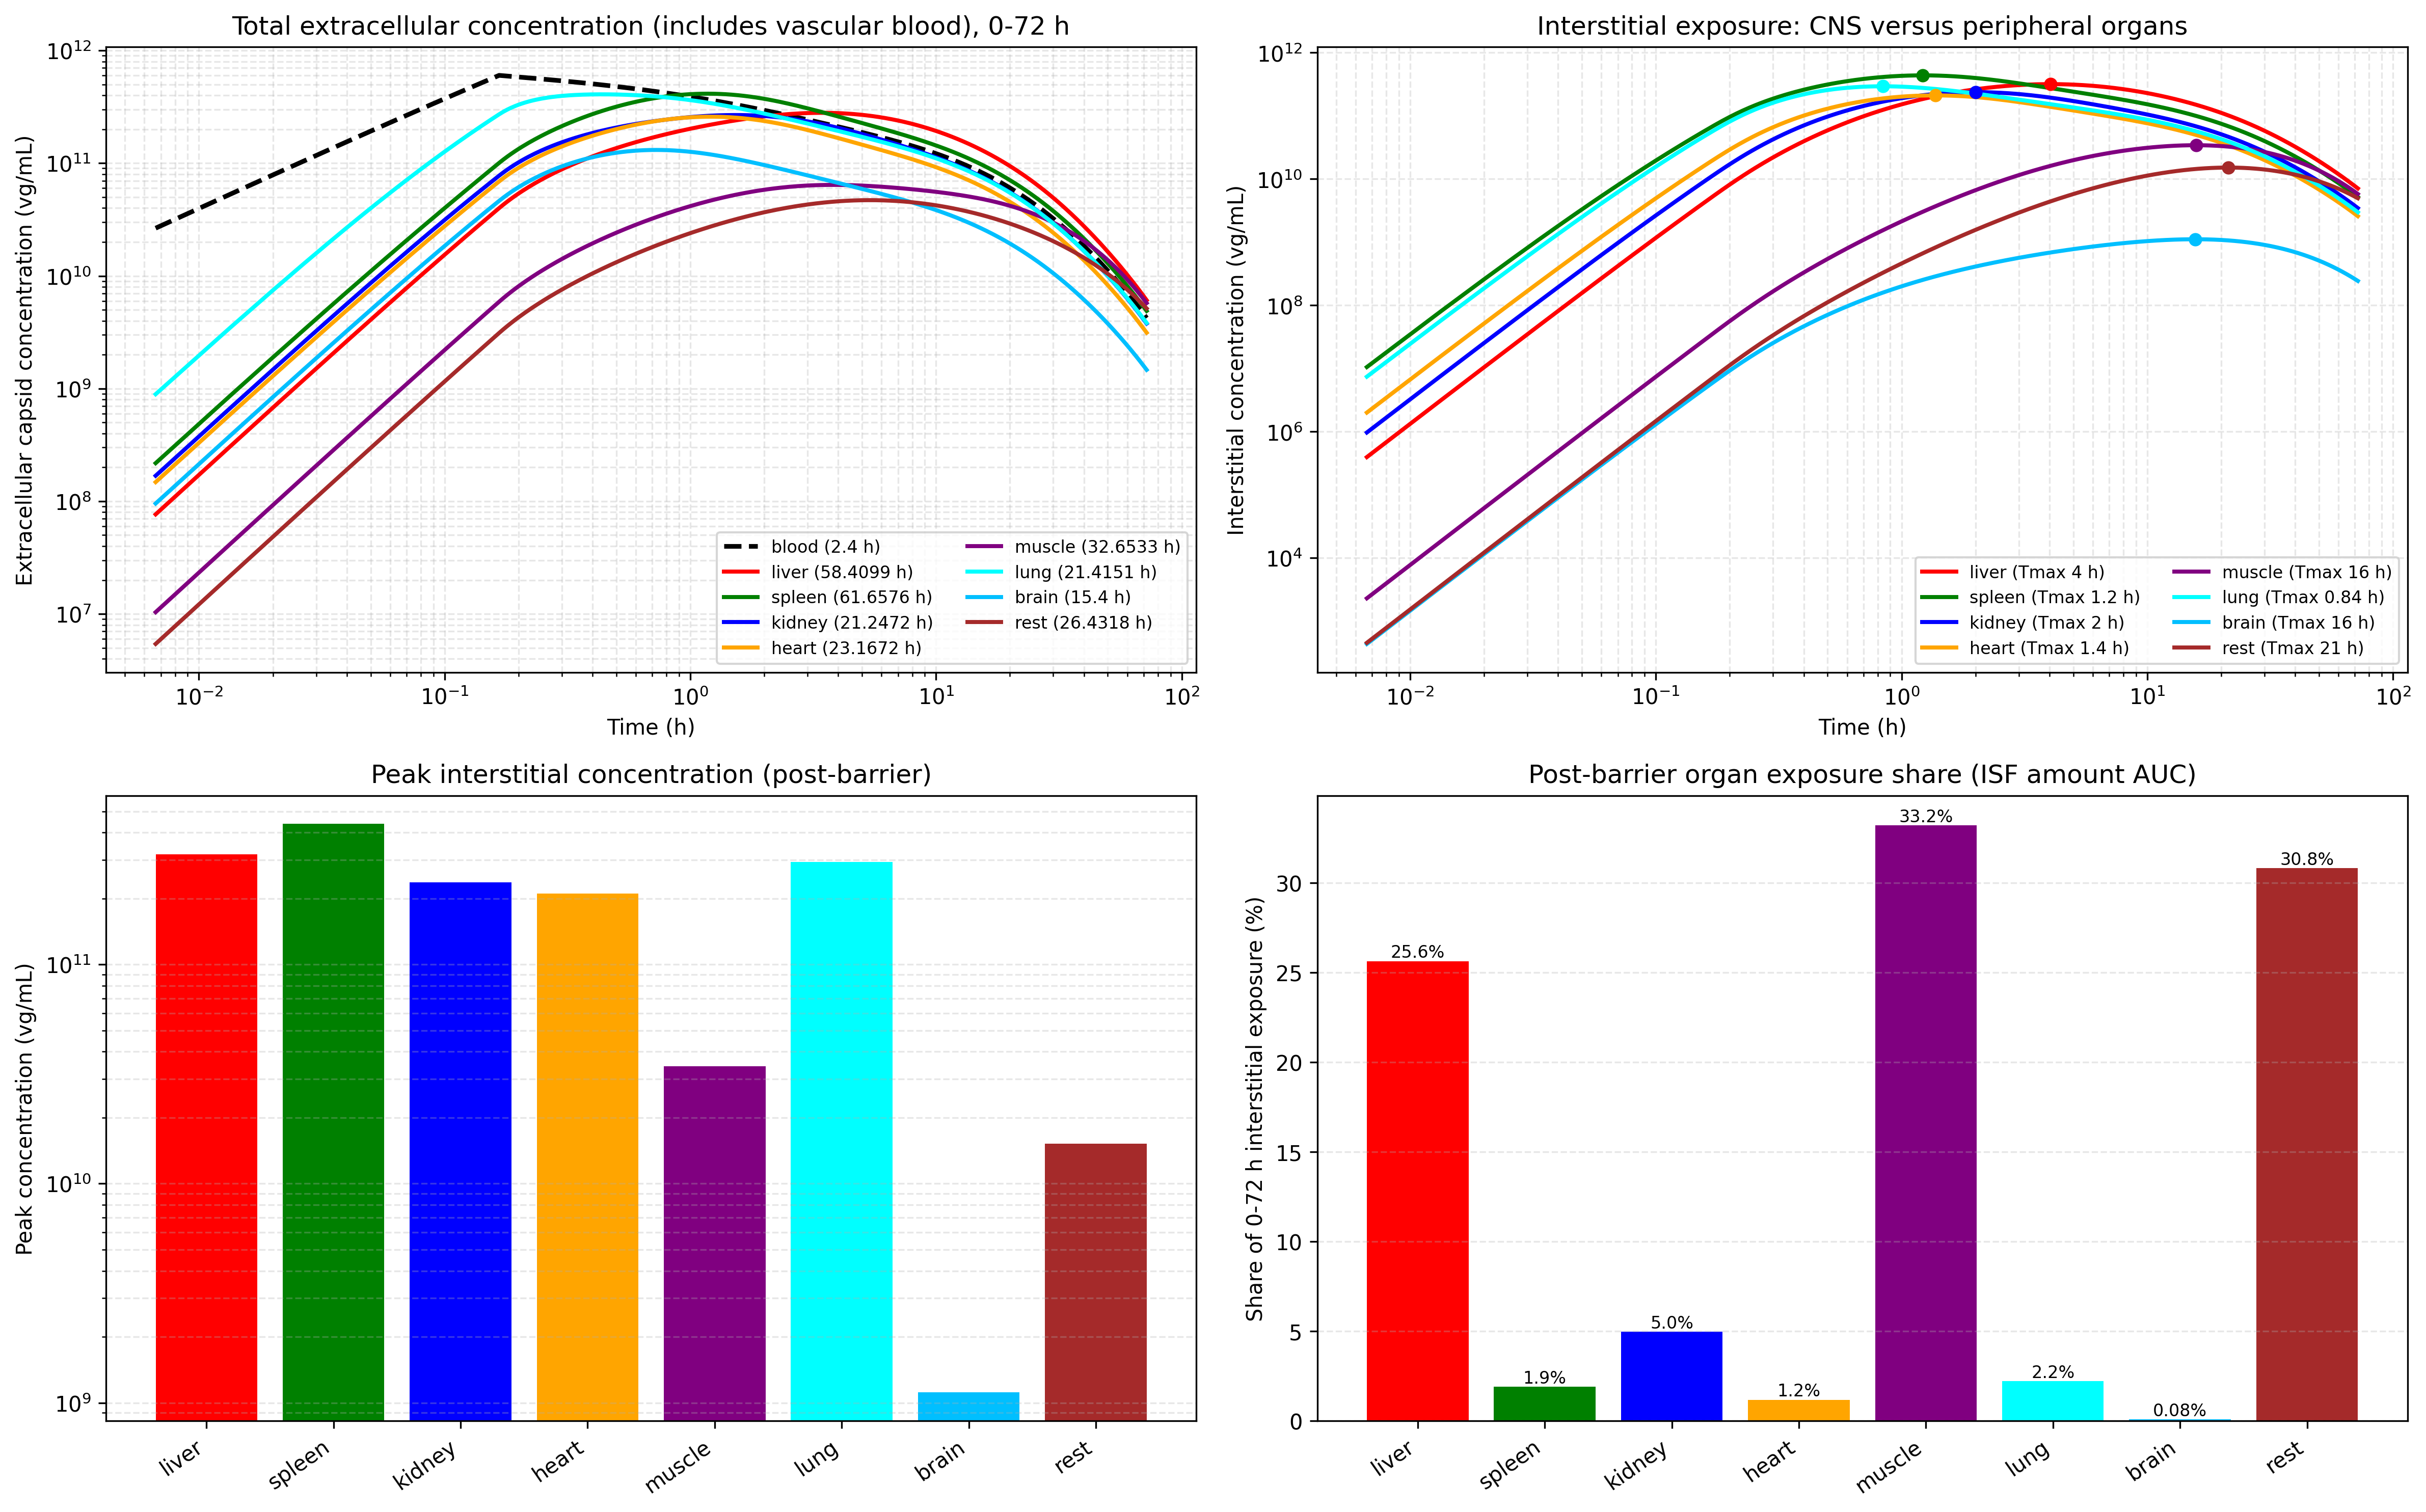
\includegraphics[width=\linewidth]{13_normal_aav9_organ_concentration_comparison_log_axes.png}
\caption{双对数轴。}
\end{subfigure}
\begin{subfigure}{0.49\textwidth}
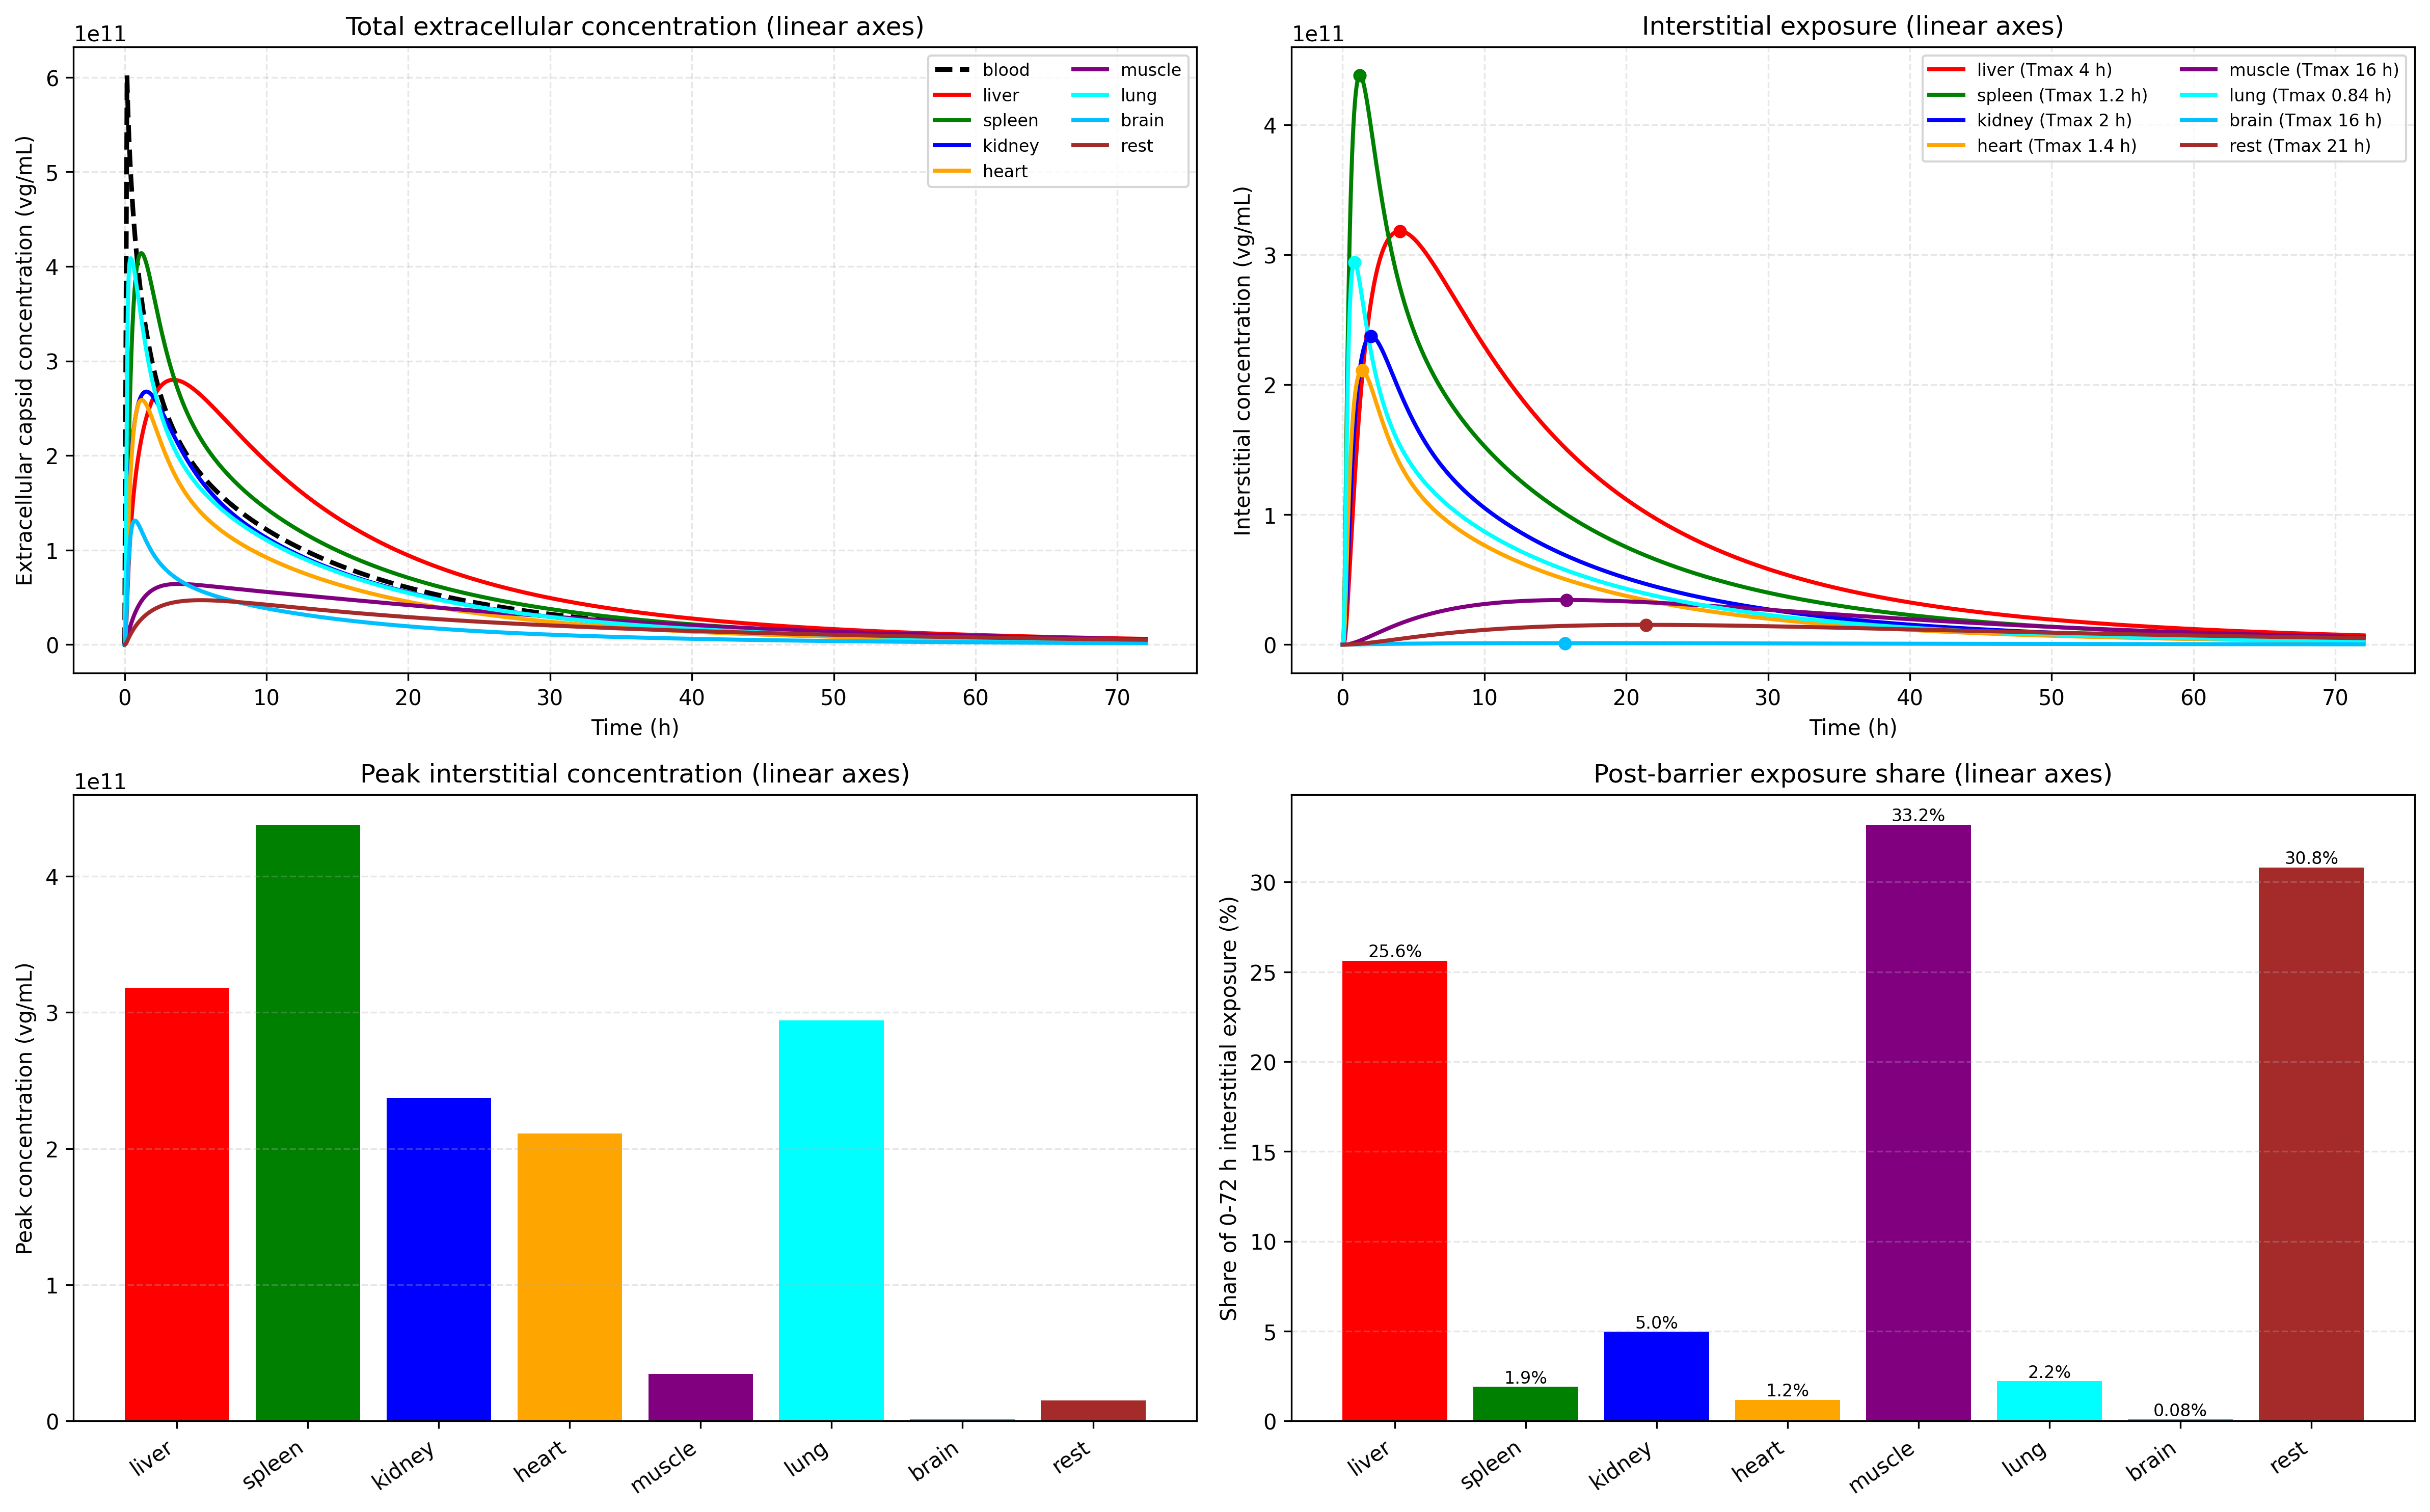
\includegraphics[width=\linewidth]{14_normal_aav9_organ_concentration_comparison_linear_axes.png}
\caption{线性轴。}
\end{subfigure}
\caption{普通 AAV9-like 基线的多器官浓度比较。对数坐标用于同时观察早期血液峰值和低暴露脑间质；另输出全线性轴版本用于直观比较绝对峰值。}
\label{fig:organ}
\end{figure}

\section{肝脏细胞转导模型}

\subsection{受体容量与摄取}
肝间质 AAV 与有限受体池结合：
\begin{align}
R_{free}&=\max(R_{tot}-B,0),\\
J_{bind}&=k_{on}C_{liver,isf}R_{free}-k_{off}B,\\
\frac{\dd B}{\dd t}&=J_{bind}-k_{int}B.
\end{align}
与单纯的一阶摄取 $kA$ 相比，该形式包含受体饱和、解离和内吞三个可独立调节环节。AAVR 已被证明是多种 AAV 血清型感染的重要宿主受体\cite{pillay2016}，但本模型的 $R_{tot}$ 是一个 lumped effective receptor capacity，尚未区分 glycan attachment、AAVR、辅助受体与细胞类型。

\subsection{胞内运输链}
肝模块使用
\[
B\rightarrow EE\rightarrow LE\rightarrow CY\rightarrow Ncap
\rightarrow Nss\rightarrow Nds\rightarrow Epi
\]
描述内吞、早/晚内体、内体逃逸、胞质、核 capsid、单链基因组、双链基因组和表达性 episome。代表性方程为
\begin{align}
\dot{EE}&=k_{int}B-(k_{ee\to le}+k_{rec}+k_{deg,ee})EE,\\
\dot{LE}&=k_{ee\to le}EE-(k_{escape}+k_{lys})LE,\\
\dot{CY}&=k_{escape}LE-(k_{nuc}+k_{uncoat,cy}+k_{deg,cy})CY,\\
\dot{Nss}&=k_{uncoat,cy}CY+k_{uncoat,nuc}Ncap-(k_{ds}+k_{deg,ss})Nss,\\
\dot{Epi}&=k_{epi}Nds-(k_{loss,epi}+k_{dil})Epi.
\end{align}
该链使“衣壳进入组织”和“最终表达”不再是同一指标。尤其 $k_{escape}$ 较小时，大量 capsid 会流入溶酶体损失；提高器官暴露不一定能等比例提高表达\cite{trafficking2012,trafficking2021}。

\subsection{表达模块}
episome 驱动的转录使用 Hill 饱和函数：
\begin{align}
v_{tx}(Epi)&=k_{tx}\frac{Epi^h}{EC_{50}^h+Epi^h},\\
\dot M&=v_{tx}-k_{deg,m}M,\\
\dot P&=k_{tl}M-k_{deg,p}P.
\end{align}
当前 $t_{1/2,m}=6$ h、$t_{1/2,p}=48$ h，因此 $k_{deg,m}=\ln2/6$ h$^{-1}$、$k_{deg,p}=\ln2/48$ h$^{-1}$。mRNA 与蛋白拥有不同量纲与数量级，最新版绘图将二者拆为独立坐标轴，避免小量级 mRNA 被蛋白曲线压扁。

\begin{figure}[H]
\centering

\includegraphics[width=0.98\textwidth]{03_liver_intracellular_56d.png}
\caption{肝脏从早期间质/受体结合到胞内运输、核内基因组处理及表达输出。左上重点显示早期峰值，右下将 mRNA 与蛋白拆轴。}
\end{figure}

\section{肾近端小管多层模型}

\subsection{为什么采用双入口}
完整 AAV capsid 的尺寸使其大量自由通过肾小球并不合理。因此模型将肾转导分成两条路径：
\begin{enumerate}
  \item \textbf{受限滤过--管腔顶端路径：}肾血管 $\to$ 少量 apparent filtrate $\to$ 近端小管管腔 $\to$ 顶端受体结合；
  \item \textbf{间质--基底外侧路径：}肾血管 $\to$ 肾 ISF $\to$ 近端小管细胞基底外侧结合。
\end{enumerate}
滤过通量与尿排写为
\begin{align}
J_{filter}&=k_{filter}A_{kidney,v},\\
J_{filtrate\to PT}&=k_{f\to pt}K_{filtrate},\\
J_{urine}&=k_{urine}K_{lumen}.
\end{align}
顶端和基底外侧结合均采用有限容量形式，例如
\begin{equation}
J_{bind,ap}=k_{on,ap}C_{lumen}(B_{max,ap}-B_{ap})-k_{off,ap}B_{ap}.
\end{equation}
顶端路径可被视为 megalin/cubilin-like lumped uptake，但当前不能声称已识别具体 AAV 受体；megalin/cubilin 主要提供近端小管受体介导内吞的结构依据\cite{megalin2002}。

\subsection{回收、溶酶体和表达}
两条入口汇入 $K_{EE}$，随后分流至回收内体 $K_{REC}$、晚期内体 $K_{LE}$、溶酶体 $K_{LYS}$ 或胞质逃逸。回收池返回管腔，尿排累计进入 $K_{Urine}$，所有胞内降解累计进入 $K_{Deg}$。这一结构能分别回答“进入肾脏”“进入近端小管细胞”“形成 episome”和“最终表达”四个层次的问题。

\begin{figure}[H]
\centering

\includegraphics[width=0.98\textwidth]{06_kidney_multilevel_module.png}
\caption{肾近端小管双入口与胞内命运。左上聚焦 0--96 h 的早期峰值；右下 mRNA 与蛋白分轴显示。}
\end{figure}

基线仿真中，肾 ISF amount AUC 为 $3.269\times10^{12}$ vg-equivalent$\cdot$h，约为肝 ISF amount AUC 的 0.532；峰值肾 episome 为 $1.038\times10^5$。以上为当前参数下的模型内部量，不应直接解释为真实动物组织中完整且仍具有感染能力的 AAV 数量。

\section{BBB 与 CNS 转导模型}

\subsection{脑器官室与 BBB}
全身 PBPK 中新增脑血管 $A_{brain,v}$ 与脑间质 $A_{brain,isf}$。普通 AAV9 基线设置较小被动 $PS_{brain}$，并用独立 BBB 受体介导路径表示结合、内吞、跨胞转运、回收和降解：
\begin{align}
J_{BBB,bind}&=k_{on,BBB}C_{brain,v}(B_{max,BBB}-B_{BBB})-k_{off,BBB}B_{BBB},\\
\dot B_{BBB}&=J_{BBB,bind}-k_{int,BBB}B_{BBB},\\
\dot E_{BBB}&=k_{int,BBB}B_{BBB}-(k_{trans}+k_{recycle}+k_{deg,BBB})E_{BBB}.
\end{align}
其中 $k_{trans}E_{BBB}$ 进入脑 ISF，$k_{recycle}E_{BBB}$ 返回脑血管。跨 BBB 后，AAV 再经历 CNS 细胞受体结合、内吞、内体逃逸、入核、解包和 episome 形成，与肝/肾共享相同的机制骨架，但拥有独立参数。

\begin{figure}[H]
\centering
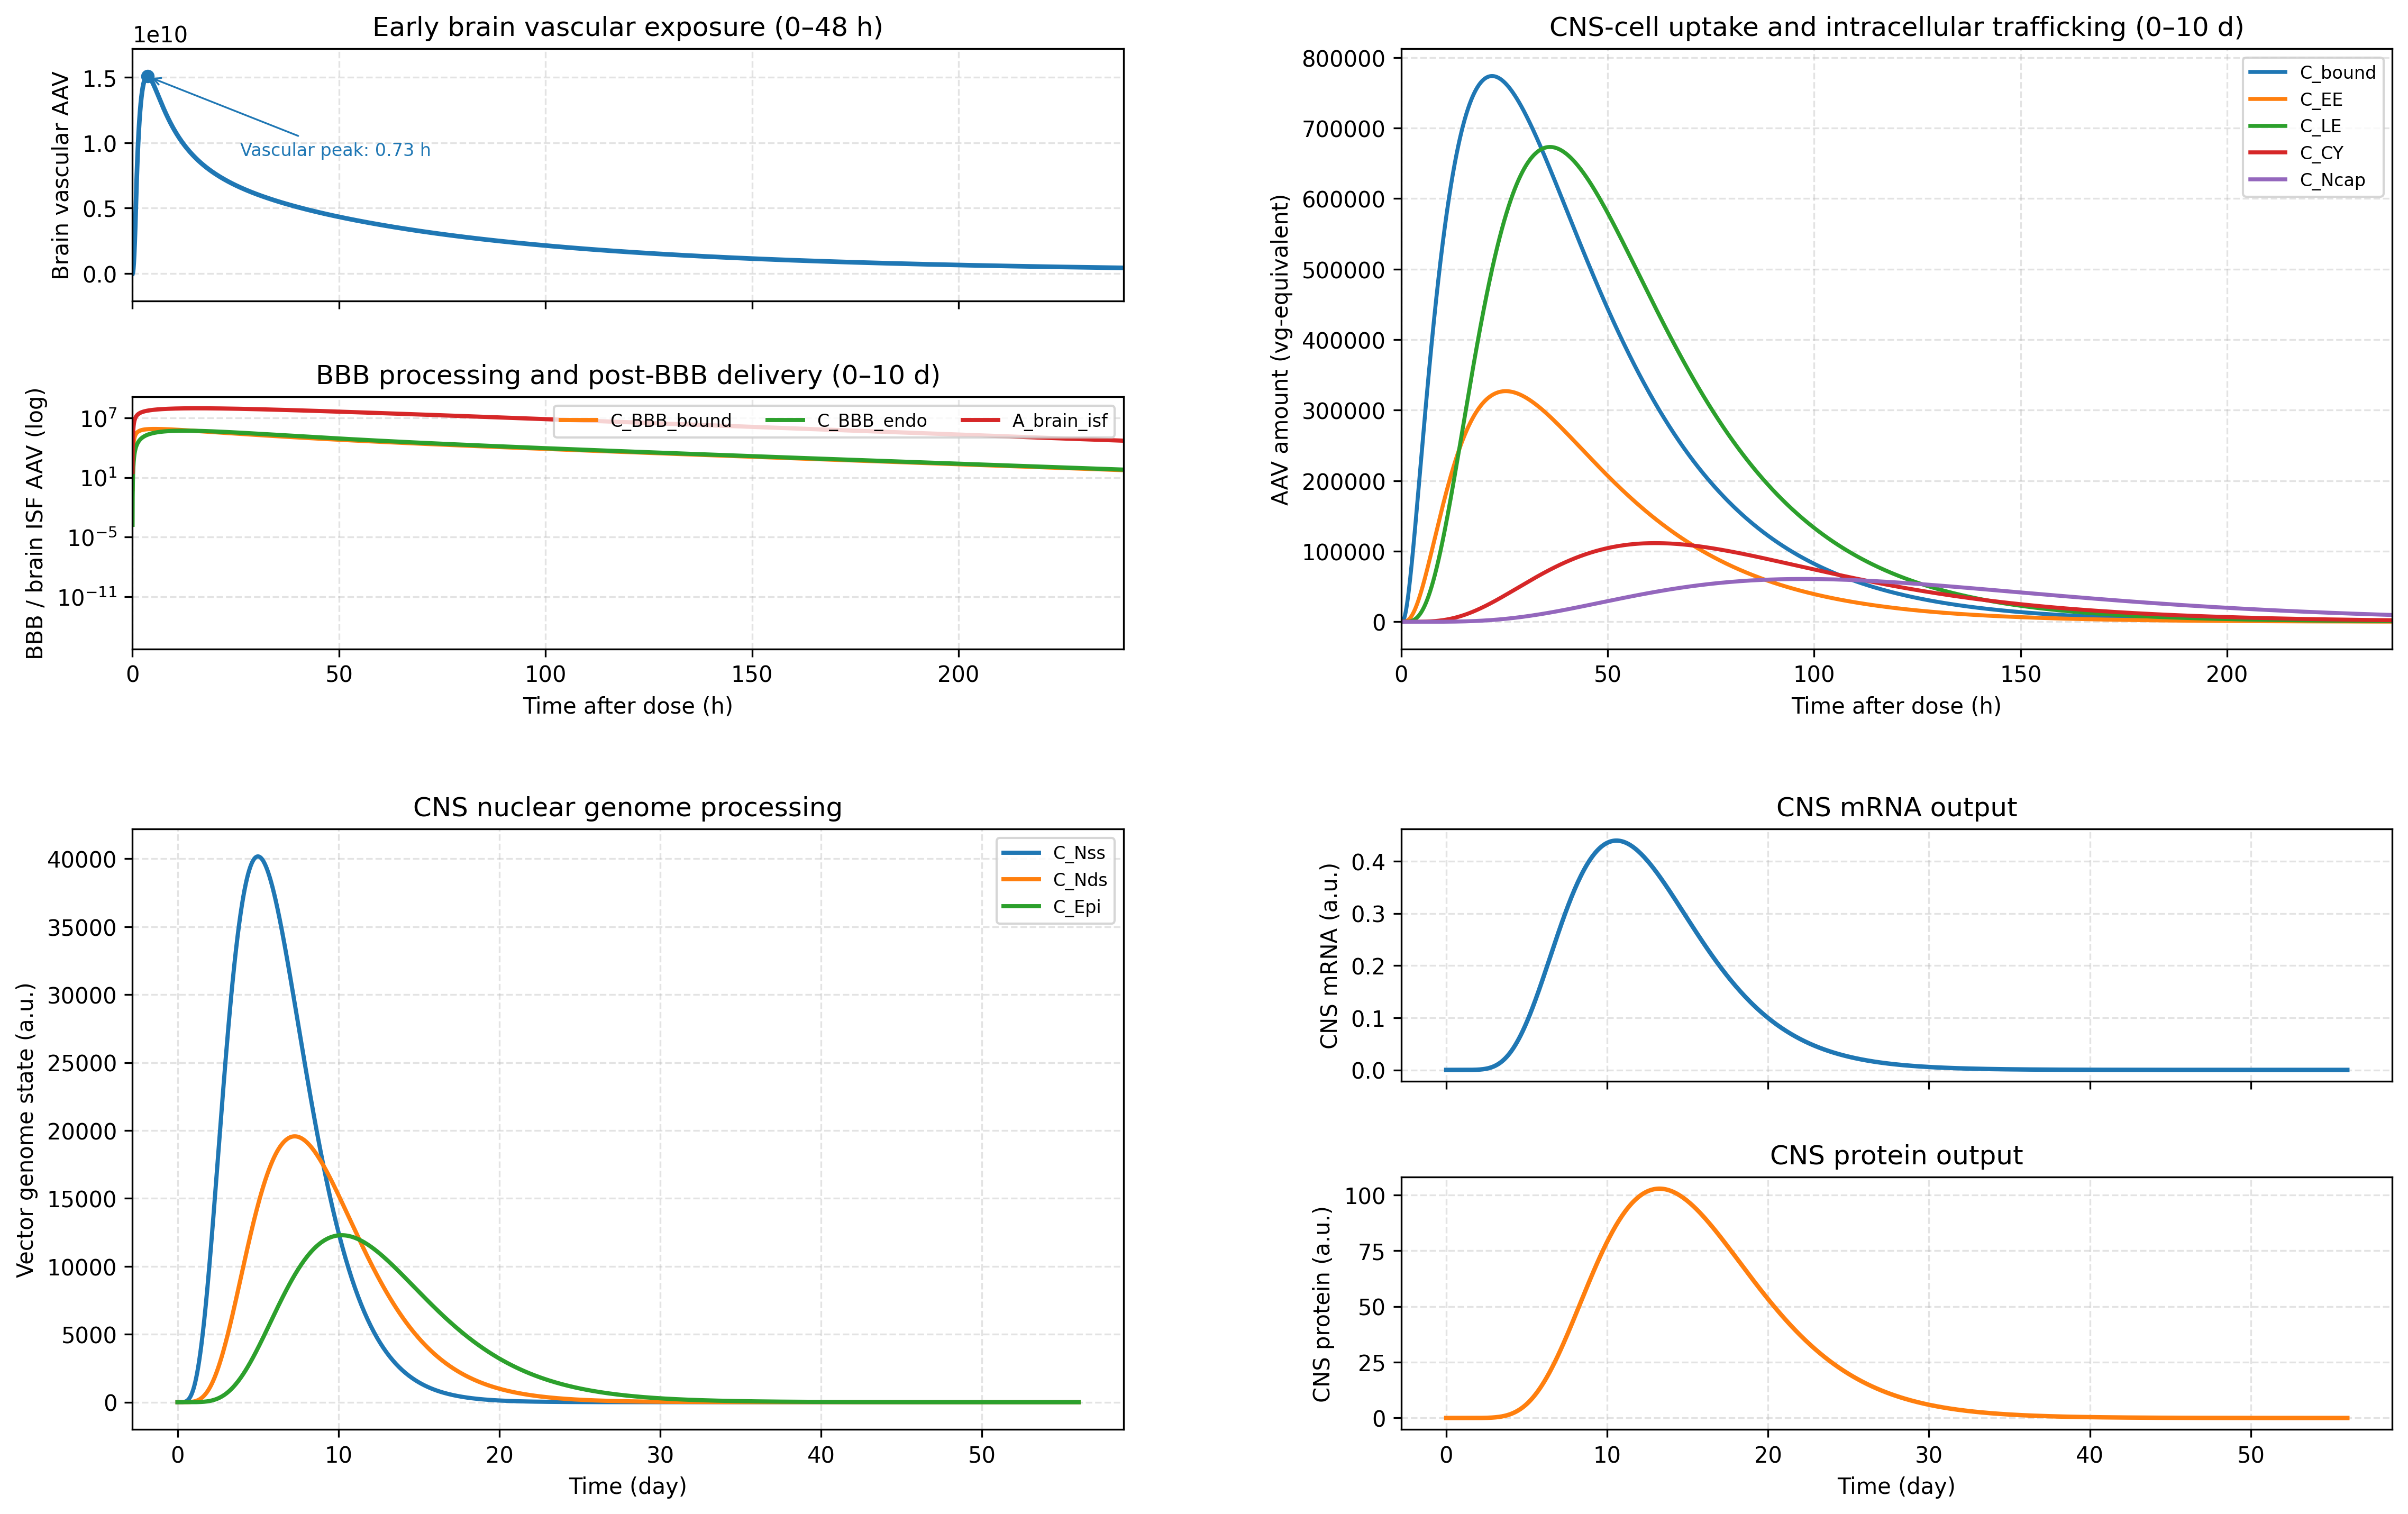
\includegraphics[width=0.98\textwidth]{11_cns_bbb_and_transduction.png}
\caption{CNS 模块输出。脑血管早期峰与 BBB/脑间质小量级状态分开显示；BBB/ISF 使用对数纵轴；mRNA 与蛋白独立成图。}
\end{figure}

基线模型得到脑 ISF amount AUC $5.677\times10^{10}$ vg-equivalent$\cdot$h，约为肝 ISF amount AUC 的 0.92\%；峰值 CNS episome 为 $1.229\times10^4$，峰值蛋白信号为 102.79 a.u.。在演示性的 CNS-tropic 参数组合下，BBB/CNS capsid 增强将峰值 CNS episome 提高到约 $1.336\times10^6$；再叠加 CNS-biased promoter 后，峰值 CNS 蛋白信号达到约 $5.697\times10^3$。这些比较说明屏障跨越、细胞内逃逸和表达调控是可叠加但不等价的设计杠杆。

\subsection{BBB 后三级深度模型}
为了让不同 CNS 疾病不再共享同一套“脑数据”，批量导出器在 $A_{brain,isf}(t)$ 之后继续求解浅表/血管周围层 $S$、皮层实质 $C$ 和深部核团 $D$：
\begin{align}
\dot S &=0.55\,u(t)-(0.18+0.08)S+0.025C,\\
\dot C &=0.18S-(0.025+0.025+0.035)C+0.012D,\\
\dot D &=0.025C-(0.012+0.050)D,
\end{align}
其中 $u(t)=A_{brain,isf}(t)/D_{dose}$。疾病/细胞类型 $j$ 的可接近信号为
\begin{equation}
X_j(t)=a_j\left(w_{S,j}S+w_{C,j}C+w_{D,j}D\right),
\end{equation}
再进入 reduced binding--endosome--cytosol--nucleus--episome ODE。不同 profile 拥有不同深度权重、cell-access factor、目标深度和持久性修正。例如 cortical excitatory 偏浅层和皮层，deep striatal 与 hypothalamic 偏深层，neural progenitor 还加入较低持久性因子。

\assumption{当前三级深度是 reduced-order compartment model，不是脑解剖网格，也没有显式细胞迁移、轴突运输、CSF 循环或区域血流。它用于产生可解释的疾病间差异，并作为未来 3D 模型的降阶原型。}

\section{SINEUP 药效动力学与持久性}

前端的“持续时间”不是直接由一个手填分数给出，而是由 PBPK/胞内 ODE 输出的相对 episome 递送信号驱动一个 0--730 d 的 SINEUP-PD 模型。对同一器官/同一 CNS profile，先将各衣壳的 episome AUC 归一化：
\begin{equation}
E_0=\frac{\AUC_{Epi,capsid}}{\max_c\AUC_{Epi,c}}.
\end{equation}
随后求解
\begin{align}
\dot E &=-k_{loss,E}E,\qquad k_{loss,E}=\frac{\ln2}{t_{1/2,E}},\\
\dot S_{RNA}&=k_{S}\frac{E}{EC_{50,E}+E}-k_{deg,S}S_{RNA},\\
G(S_{RNA})&=G_{max}\frac{S_{RNA}}{EC_{50,S}+S_{RNA}},\\
P_{set}&=\min\left[1,\,0.5(1+G)\right],\\
\dot P&=k_{turn}(P_{set}-P).
\end{align}
基线将单倍剂量不足的蛋白设为 50\%，当预测蛋白达到 65\% 以上时计入有效治疗窗口。网页纵轴使用最后一次高于 65\% 阈值的时间作为 \code{effective\_duration\_days}。当前 SINEUP RNA 半衰期为 0.25 d，目标蛋白半衰期为 2 d，episome 半衰期由器官先验和衣壳 persistence factor 决定。

这套结构的重要意义在于：纵轴同时受初始递送、episome 保持、SINEUP RNA 周转和内源蛋白周转影响，而不是简单把 capsid 半衰期当成疗效持续时间。

\section{数值求解、时间网格与质量守恒}

\subsection{积分策略}
ODE 使用 SciPy \code{solve\_ivp} 的刚性求解器 BDF。由于 10 min 输注终点导致输入函数不连续，模型在 $T_{inf}$ 处分段积分，并对早期时间使用更密集网格。短期网格用于观察分钟至小时的分布峰，长期网格延伸至 56 d 用于观察 episome、mRNA 和蛋白动态。批量衣壳计算使用 0--72 h 网格，以控制前端数据生成成本。

\subsection{质量守恒审计}
定义所有仍存在的 AAV 状态与累计损失 sink 之和为 $A_{accounted}$：
\begin{align}
A_{accounted}={}&A_{extracellular}+A_{liver,vector}+A_{kidney,vector}+A_{CNS,vector}\\
&+K_{Urine}+K_{Deg}+C_{Deg}+L_{blood}+L_{vascular}+L_{ISF}+L_{neut}+L_{liver}.
\end{align}
相对误差为
\begin{equation}
\epsilon_{mass}(t)=\frac{A_{accounted}(t)-Dose_{in}(t)}{\max(Dose_{in}(t),10^{-30})}.
\end{equation}
基线完整运行的最终误差为 $-3.418\times10^{-15}$，不同设计场景保持在 $10^{-14}$ 数量级。这证明 ODE 状态转移与累计 sink 在数值上闭合，但\textbf{质量守恒不能替代参数校准或生物学验证}。

\begin{figure}[H]
\centering

\includegraphics[width=0.84\textwidth]{08_mass_balance_audit.png}
\caption{质量守恒审计输出。模型将清除和降解作为显式累计状态，而不是让向量从方程中无去向地消失。}
\end{figure}

\section{衣壳与启动子场景比较}

主模型提供 capsid 与 promoter 两层 preset。capsid 层可改变器官 $PS/K_p$、受体结合、BBB 跨越和内体逃逸；promoter 层只改变 episome 之后的组织表达参数。这样可以避免把“送得更多”和“表达得更多”混成同一个参数。

\begin{table}[H]
\centering
\caption{当前主模型场景结果摘要。数值是模型单位，用于场景内比较。}
\begin{tabularx}{\textwidth}{lrrrr}
\toprule
场景 & 肝峰值 Epi & 肾峰值 Epi & 肝峰值蛋白 & 肾峰值蛋白 \\
\midrule
Baseline & 4,683 & 103,806 & 5,913 & 3,588 \\
Liver detargeted & 2,798 & 100,847 & 5,854 & 3,587 \\
Kidney tropic + kidney promoter & 4,679 & 357,155 & 2,661 & 6,229 \\
Endosomal escape enhanced & 11,562 & 247,864 & 5,962 & 3,592 \\
\bottomrule
\end{tabularx}
\end{table}

例如，增强内体逃逸显著提高了肝和肾 episome，但由于表达 Hill 函数接近饱和，峰值蛋白并未等比例提高。这是机制模型相对于线性评分的优势：它能揭示某个优化是否已被下游瓶颈“截断”。

\begin{figure}[H]
\centering

\includegraphics[width=0.9\textwidth]{09_design_scenario_comparison.png}
\caption{基线、肝脱靶、肾嗜性和内体逃逸增强场景的比较。}
\end{figure}

\section{二维设计空间与疾病数据库}

\subsection{从 ODE 输出到二维坐标}
每个“目标器官/细胞 profile--衣壳”组合形成一个点。横轴是器官特异性：
\begin{equation}
S_{organ}=\log_{10}\left(
\frac{\AUC(C_{target,isf})}
{\operatorname{mean}_{i\ne target}[w_i\AUC(C_{i,isf})]}
\right),
\end{equation}
其中 $w_i$ 是脱靶毒性权重。纵轴是上一节 SINEUP-PD 数值求解得到的有效持续时间。点的详情还显示峰值 post-barrier delivery、目标暴露份额、tmax、证据等级、物种来源、转导模型类型和质量守恒误差。

背景色不是额外修改计算结果，而是把二维空间划分为四个设计语义区：
\begin{itemize}
  \item 高特异性、长持续：优先候选；
  \item 高特异性、短持续：适合需要可逆性或可重复给药的情况；
  \item 低特异性、长持续：需警惕长期脱靶表达；
  \item 低特异性、短持续：通常效用较低。
\end{itemize}

\subsection{衣壳先验与证据标签}
当前数据库包含 AAV2、AAV5、AAV8、AAV9、AAVrh.10、PHP.eB、CAP-B10 和 AAV-LK03。先验通过缩放器官 $PS_i$、$K_{p,i}$ 和 BBB transcytosis 映射到 PBPK，而不是直接手填最终二维坐标。不同来源跨越 mouse、NHP、human-hepatocyte prior 和临床/局部眼科证据，因此前端明确显示 strong、medium、exploratory，并保留 source 链接。PHP.eB 等衣壳的物种依赖尤其需要显著提示，不能将特定小鼠受体背景中的 CNS 嗜性直接外推到人。

\subsection{疾病--基因层级库}
疾病库采用“疾病列表--展开基因”的层级结构。Wolf--Hirschhorn syndrome 不再是单一记录，而是包含 NSD2、LETM1、WHSC1/相关区段基因和 CPLX1 等多个候选靶点；同时加入 CHD8、SCN1A/Dravet、SHANK3/Phelan--McDermid、EHMT1/Kleefstra、RAI1/Smith--Magenis、NSD1/Sotos、SATB2、MEF2C、FOXP1、TCF4、SYNGAP1、DYRK1A、NRXN1、PAFAH1B1、ANKRD11 等单倍剂量不足或缺失相关疾病。每条记录包含 locus、目标器官、目标细胞、机制、残余等位基因要求、注意事项和 ClinGen 证据入口。

CNS 疾病会进一步映射到 cortical excitatory、cortical inhibitory、cortical projection、synaptic neuron、deep striatal、hypothalamic、broad neuronal 或 neural progenitor profile。于是同一衣壳在不同疾病中会因目标深度和细胞可接近性而得到不同的特异性及持续性，不再是一套数据复用。

\subsection{前端实现与数据来源证明}
前端采用中英文切换、独立可滚动疾病库、可展开疾病组、全部衣壳切换、模型/代理标签和证据卡。数据文件由 \code{export\_delivery\_design\_space.py} 批量运行 \code{ode1.0.py} 后生成 JSON/CSV；页面只负责筛选和可视化，不在浏览器中重新编造分数。模型生成时间固定为 UTC 字符串，避免服务端和客户端使用本地时区格式化造成 React hydration mismatch。

\section{Spatial PK 与流体力学路线}

\subsection{已完成的一维演示}
当前一维模型在归一化血管/组织轴 $x$ 上求解对流--扩散--受体摄取：
\begin{equation}
\frac{\partial C}{\partial t}+u\frac{\partial C}{\partial x}
=D\frac{\partial^2C}{\partial x^2}-J_{uptake}(C,B),
\end{equation}
并在每个网格点计算
\begin{align}
\dot B&=k_{on}C(B_{max}-B)-k_{off}B-k_{int}B,\\
\dot I&=k_{int}B-k_{escape}I-k_{lys}I,\\
\dot E&=k_{escape}I-k_{loss,E}E.
\end{align}
入口边界 $C(0,t)$ 来自 0D PBPK 的血液浓度曲线。演示比较 baseline IV-like、capsid wall-access enhanced 和 slow-flow local trapping，说明即使总给药相同，流速、停留时间和壁面摄取也会改变最终 episome 的空间均匀度。

\begin{figure}[H]
\centering

\includegraphics[width=0.88\textwidth]{10_spatial_pk_1d_demo.png}
\caption{一维 spatial PK 演示：PBPK 作为入口边界，局部流动和壁面摄取共同塑造表达性 episome 的空间分布。}
\end{figure}

\subsection{未来 3D CNS 模型}
下一阶段可建立从血管到脑实质的 3D advection--diffusion--reaction 模型：
\begin{align}
\nabla\cdot\bm u&=0,\\
\rho\left(\frac{\partial\bm u}{\partial t}+\bm u\cdot\nabla\bm u\right)&=-\nabla p+\mu\nabla^2\bm u,\\
\frac{\partial C}{\partial t}+\nabla\cdot(\bm uC)&=\nabla\cdot(D\nabla C)-R_{uptake}(C,\bm x).
\end{align}
推荐分四步实施：
\begin{enumerate}
  \item 用理想化毛细血管--周血管--实质圆柱几何完成 2D axisymmetric 原型；
  \item 将 BBB 通量设为 Robin 边界，参数由当前 ODE 的 $k_{BBB}$ 和受体容量转换；
  \item 加入脑区分层的扩散系数、细胞密度、受体密度和外排/降解；
  \item 使用成像或组织切片校准空间参数，再导出降阶参数回填网页的 CNS profile。
\end{enumerate}
若有 MRI/血管图谱，可进一步构建个体化几何；若没有，先用理想化微血管单元比直接上全脑网格更容易验证。对 CSF 或局部脑内给药，还需加入 CSF bulk flow、pulsatility 和 perivascular transport。PET 研究表明，即使向 CSF 给药，也可能有显著系统外流和外周器官暴露，因此未来模型必须同时保留 CNS 与全身收支\cite{csfpet2023}。

\section{湿实验闭环}

\begin{table}[H]
\centering
\caption{模型参数、可测量数据与实验反馈关系。}
\begin{tabularx}{\textwidth}{p{0.22\textwidth}p{0.30\textwidth}X}
\toprule
模型环节 & 推荐实验 & 可校准参数/判别问题 \\
\midrule
血液与器官分布 & 血浆及肝/脾/肾/心/肌/肺/脑 qPCR 或 ddPCR 时间序列 & $Q_i,PS_i,K_{p,i},k_{clear}$；区分早期分布与后期残留 \\
完整 capsid 命运 & capsid ELISA/免疫染色、放射或荧光标记成像 & 表观 capsid PK；避免仅用 vg 信号解释完整病毒 \\
细胞类型摄取 & 组织切片与 hepatocyte、Kupffer、PT、endothelium、neuron/glia marker 共定位 & $B_{max},k_{on},k_{int}$ 及细胞类型份额 \\
胞内运输 & 亚细胞分级、内体/溶酶体/核共定位 & $k_{escape},k_{lys},k_{nuc},k_{uncoat}$ \\
episome & 核内 vector genome、双链/环状 episome 测定 & $k_{ds},k_{epi},k_{loss,Epi}$ \\
SINEUP RNA & RT-qPCR、RNA half-life、构建特异表达 & $k_{S},k_{deg,S}$，不同 SINEUP 元件比较 \\
蛋白恢复 & western blot、ELISA、功能 readout & 翻译增益、蛋白周转、65\% 阈值的生物学合理性 \\
空间分布 & 全器官成像、分区取样、空间转录/蛋白检测 & $D,u,R_{uptake}$ 与 CNS 深度权重 \\
免疫 & NAb、补体、细胞因子及重复给药实验 & $k_{neut}$、免疫清除和重复给药限制 \\
\bottomrule
\end{tabularx}
\end{table}

推荐最小闭环是：先选择 2--3 个衣壳、1 个报告系统和肝/肾/脑三个组织，在 0.5 h、2 h、8 h、24 h、72 h、7 d 和 28 d 取样。早期测 vector/capsid，后期测 episome、RNA 和蛋白。用早期数据拟合 PBPK 与摄取，用后期数据拟合表达和持久性，再重新生成二维点图。这样网页中的候选排序会随实验数据更新，而不是停留在固定文献先验。

\section{完整参数注册表与证据等级}

下表由 \code{python model/export\_parameter\_registry.py} 从实际代码生成。\textbf{direct} 表示直接转录，\textbf{fitted} 表示由源数据拟合，\textbf{derived} 表示由有来源的量计算，\textbf{scaled} 表示跨区域/物种转化，\textbf{assumed} 表示当前数值是透明先验。一个参数可以具有文献支持的机制，但数值仍为 assumed；例如 AAVR 和内体运输有充分机制依据，却没有为本构建拟合出 \code{k\_on} 或 \code{k\_escape}。

\IfFileExists{generated_parameter_table.tex}{%
  \begingroup\scriptsize\sloppy
\setlength{\tabcolsep}{2.5pt}
\begin{longtable}{>{\raggedright\arraybackslash}p{0.10\textwidth}>{\raggedright\arraybackslash}p{0.13\textwidth}>{\raggedright\arraybackslash}p{0.15\textwidth}>{\raggedright\arraybackslash}p{0.08\textwidth}>{\raggedright\arraybackslash}p{0.11\textwidth}>{\raggedright\arraybackslash}p{0.11\textwidth}>{\raggedright\arraybackslash}p{0.22\textwidth}}
\caption{完整中英双语模型参数注册表。evidence type 区分 direct、fitted、derived、scaled 与 assumed；assumed 不表示机制没有依据，而表示当前数值尚未由本项目数据校准。}\label{tab:all-parameters}\\
\toprule Scope / 范围 & Parameter & Description / 描述 & Value & Unit & Evidence / 证据 & Reference / rationale / 参考与理由 \\
\midrule\endfirsthead
\toprule Scope / 范围 & Parameter & Description / 描述 & Value & Unit & Evidence / 证据 & Reference / rationale / 参考与理由 \\
\midrule\endhead
\midrule\multicolumn{7}{r}{Continued on next page}\\\endfoot
\bottomrule\endlastfoot
mouse\_\allowbreak{}pbpk /\allowbreak{} 小鼠 PBPK & Bmax\_\allowbreak{}bbb & BBB binding, traffic\allowbreak{}king or capacity paramet\allowbreak{}er /\allowbreak{} 血脑屏障结合、转运或容量参数 & 1e+07 & mixed; see equation /\allowbreak{} 混合单位，见对应方程 & assumed /\allowbreak{} 假设值 & Nonnenm\allowbreak{}acher and Weber 2012, doi:\allowbreak{}10.1038/\allowbreak{}gt.2012.6; Riyad and Weber 2021, doi:\allowbreak{}10.1038/\allowbreak{}s41434-021-00243-z. BBB mechani\allowbreak{}sm is represe\allowbreak{}nted explici\allowbreak{}tly; numeric\allowbreak{}al rate is not fitted /\allowbreak{} 显式表示 BBB 机制，但数值速率尚未拟合 \\
mouse\_\allowbreak{}pbpk /\allowbreak{} 小鼠 PBPK & Bmax\_\allowbreak{}cns & CNS-cell uptake, traffic\allowbreak{}king or express\allowbreak{}ion paramet\allowbreak{}er /\allowbreak{} CNS 细胞摄取、转运或表达参数 & 3e+07 & mixed; see equation /\allowbreak{} 混合单位，见对应方程 & assumed /\allowbreak{} 假设值 & Nonnenm\allowbreak{}acher and Weber 2012, doi:\allowbreak{}10.1038/\allowbreak{}gt.2012.6; Riyad and Weber 2021, doi:\allowbreak{}10.1038/\allowbreak{}s41434-021-00243-z. Transfe\allowbreak{}rred intrace\allowbreak{}llular chain with CNS-specific explora\allowbreak{}tory values /\allowbreak{} 沿用胞内转运链，并采用 CNS 特异的探索性数值 \\
mouse\_\allowbreak{}pbpk /\allowbreak{} 小鼠 PBPK & Bmax\_\allowbreak{}pt\_\allowbreak{}apical & Kidney filtrat\allowbreak{}ion, proximal-tubule uptake or traffic\allowbreak{}king paramet\allowbreak{}er /\allowbreak{} 肾滤过、近端小管摄取或转运参数 & 5e+07 & mixed; see equation /\allowbreak{} 混合单位，见对应方程 & assumed /\allowbreak{} 假设值 & Christe\allowbreak{}nsen and Birn 2002, doi:\allowbreak{}10.1038/\allowbreak{}nrm778 (mechani\allowbreak{}stic proximal-tubule endocyt\allowbreak{}osis only). Dual-entry mechani\allowbreak{}sm is biologi\allowbreak{}cally motivat\allowbreak{}ed; intact-AAV rates remain provisi\allowbreak{}onal /\allowbreak{} 双入口机制具有生物学依据，但完整 AAV 的速率仍为暂定值 \\
mouse\_\allowbreak{}pbpk /\allowbreak{} 小鼠 PBPK & Bmax\_\allowbreak{}pt\_\allowbreak{}bsl & Kidney filtrat\allowbreak{}ion, proximal-tubule uptake or traffic\allowbreak{}king paramet\allowbreak{}er /\allowbreak{} 肾滤过、近端小管摄取或转运参数 & 2e+07 & mixed; see equation /\allowbreak{} 混合单位，见对应方程 & assumed /\allowbreak{} 假设值 & Christe\allowbreak{}nsen and Birn 2002, doi:\allowbreak{}10.1038/\allowbreak{}nrm778 (mechani\allowbreak{}stic proximal-tubule endocyt\allowbreak{}osis only). Dual-entry mechani\allowbreak{}sm is biologi\allowbreak{}cally motivat\allowbreak{}ed; intact-AAV rates remain provisi\allowbreak{}onal /\allowbreak{} 双入口机制具有生物学依据，但完整 AAV 的速率仍为暂定值 \\
mouse\_\allowbreak{}pbpk /\allowbreak{} 小鼠 PBPK & CL\_\allowbreak{}blood & Model paramet\allowbreak{}er /\allowbreak{} 模型参数 & 0 & see code /\allowbreak{} 见代码 & assumed /\allowbreak{} 假设值 & Current model structu\allowbreak{}ral prior; requires project-specific calibra\allowbreak{}tion. Retained for full auditab\allowbreak{}ility /\allowbreak{} 为完整审计而保留 \\
mouse\_\allowbreak{}pbpk /\allowbreak{} 小鼠 PBPK & CO & Referen\allowbreak{}ce cardiac output /\allowbreak{} 参考心输出量 & 840 & mL/\allowbreak{}h /\allowbreak{} mL/\allowbreak{}h & direct/\allowbreak{}scaled /\allowbreak{} 直接证据/\allowbreak{}缩放值 & Brown et al. 1997; Davies and Morris 1993; Shah and Betts 2012/\allowbreak{}2013. 14 mL/\allowbreak{}min referen\allowbreak{}ce for an unanest\allowbreak{}hetized 25 g mouse /\allowbreak{} 14 mL/\allowbreak{}min referen\allowbreak{}ce for an unanest\allowbreak{}hetized 25 g mouse \\
mouse\_\allowbreak{}pbpk /\allowbreak{} 小鼠 PBPK & EC50\_\allowbreak{}ab & Cellular uptake, intrace\allowbreak{}llular traffic\allowbreak{}king, immune or express\allowbreak{}ion paramet\allowbreak{}er /\allowbreak{} 细胞摄取、胞内转运、免疫或表达参数 & 1e+10 & mixed; see equation /\allowbreak{} 混合单位，见对应方程 & assumed /\allowbreak{} 假设值 & Pillay et al. 2016, doi:\allowbreak{}10.1038/\allowbreak{}nature1\allowbreak{}6465; Nonnenm\allowbreak{}acher and Weber 2012, doi:\allowbreak{}10.1038/\allowbreak{}gt.2012.6; Riyad and Weber 2021, doi:\allowbreak{}10.1038/\allowbreak{}s41434-021-00243-z. Mechani\allowbreak{}stic step is literat\allowbreak{}ure-support\allowbreak{}ed; present numeric\allowbreak{}al value is an explora\allowbreak{}tory prior /\allowbreak{} 机制步骤有文献支持，但当前数值仍是探索性先验 \\
mouse\_\allowbreak{}pbpk /\allowbreak{} 小鼠 PBPK & EC50\_\allowbreak{}cns\_\allowbreak{}tx & Cellular uptake, intrace\allowbreak{}llular traffic\allowbreak{}king, immune or express\allowbreak{}ion paramet\allowbreak{}er /\allowbreak{} 细胞摄取、胞内转运、免疫或表达参数 & 2e+05 & mixed; see equation /\allowbreak{} 混合单位，见对应方程 & assumed /\allowbreak{} 假设值 & Pillay et al. 2016, doi:\allowbreak{}10.1038/\allowbreak{}nature1\allowbreak{}6465; Nonnenm\allowbreak{}acher and Weber 2012, doi:\allowbreak{}10.1038/\allowbreak{}gt.2012.6; Riyad and Weber 2021, doi:\allowbreak{}10.1038/\allowbreak{}s41434-021-00243-z. Mechani\allowbreak{}stic step is literat\allowbreak{}ure-support\allowbreak{}ed; present numeric\allowbreak{}al value is an explora\allowbreak{}tory prior /\allowbreak{} 机制步骤有文献支持，但当前数值仍是探索性先验 \\
mouse\_\allowbreak{}pbpk /\allowbreak{} 小鼠 PBPK & EC50\_\allowbreak{}kidney\_\allowbreak{}tx & Cellular uptake, intrace\allowbreak{}llular traffic\allowbreak{}king, immune or express\allowbreak{}ion paramet\allowbreak{}er /\allowbreak{} 细胞摄取、胞内转运、免疫或表达参数 & 100 & mixed; see equation /\allowbreak{} 混合单位，见对应方程 & assumed /\allowbreak{} 假设值 & Pillay et al. 2016, doi:\allowbreak{}10.1038/\allowbreak{}nature1\allowbreak{}6465; Nonnenm\allowbreak{}acher and Weber 2012, doi:\allowbreak{}10.1038/\allowbreak{}gt.2012.6; Riyad and Weber 2021, doi:\allowbreak{}10.1038/\allowbreak{}s41434-021-00243-z. Mechani\allowbreak{}stic step is literat\allowbreak{}ure-support\allowbreak{}ed; present numeric\allowbreak{}al value is an explora\allowbreak{}tory prior /\allowbreak{} 机制步骤有文献支持，但当前数值仍是探索性先验 \\
mouse\_\allowbreak{}pbpk /\allowbreak{} 小鼠 PBPK & EC50\_\allowbreak{}tx & Cellular uptake, intrace\allowbreak{}llular traffic\allowbreak{}king, immune or express\allowbreak{}ion paramet\allowbreak{}er /\allowbreak{} 细胞摄取、胞内转运、免疫或表达参数 & 100 & mixed; see equation /\allowbreak{} 混合单位，见对应方程 & assumed /\allowbreak{} 假设值 & Pillay et al. 2016, doi:\allowbreak{}10.1038/\allowbreak{}nature1\allowbreak{}6465; Nonnenm\allowbreak{}acher and Weber 2012, doi:\allowbreak{}10.1038/\allowbreak{}gt.2012.6; Riyad and Weber 2021, doi:\allowbreak{}10.1038/\allowbreak{}s41434-021-00243-z. Mechani\allowbreak{}stic step is literat\allowbreak{}ure-support\allowbreak{}ed; present numeric\allowbreak{}al value is an explora\allowbreak{}tory prior /\allowbreak{} 机制步骤有文献支持，但当前数值仍是探索性先验 \\
mouse\_\allowbreak{}pbpk /\allowbreak{} 小鼠 PBPK & Kp\_\allowbreak{}brain & Tissue-to-plasma partiti\allowbreak{}on coeffic\allowbreak{}ient /\allowbreak{} 组织-血浆分配系数 & 0.04 & dimensi\allowbreak{}onless /\allowbreak{} 无量纲 & assumed /\allowbreak{} 假设值 & Liu et al. 2024, doi:\allowbreak{}10.1016/\allowbreak{}j.xphs.2023.10.005. Explora\allowbreak{}tory ISF exchange prior; Liu whole-tissue T/\allowbreak{}B ratios are calibra\allowbreak{}tion targets, not direct Kp replace\allowbreak{}ments /\allowbreak{} Explora\allowbreak{}tory ISF exchange prior; Liu whole-tissue T/\allowbreak{}B ratios are calibra\allowbreak{}tion targets, not direct Kp replace\allowbreak{}ments \\
mouse\_\allowbreak{}pbpk /\allowbreak{} 小鼠 PBPK & Kp\_\allowbreak{}heart & Tissue-to-plasma partiti\allowbreak{}on coeffic\allowbreak{}ient /\allowbreak{} 组织-血浆分配系数 & 0.6 & dimensi\allowbreak{}onless /\allowbreak{} 无量纲 & assumed /\allowbreak{} 假设值 & Liu et al. 2024, doi:\allowbreak{}10.1016/\allowbreak{}j.xphs.2023.10.005. Explora\allowbreak{}tory ISF exchange prior; Liu whole-tissue T/\allowbreak{}B ratios are calibra\allowbreak{}tion targets, not direct Kp replace\allowbreak{}ments /\allowbreak{} Explora\allowbreak{}tory ISF exchange prior; Liu whole-tissue T/\allowbreak{}B ratios are calibra\allowbreak{}tion targets, not direct Kp replace\allowbreak{}ments \\
mouse\_\allowbreak{}pbpk /\allowbreak{} 小鼠 PBPK & Kp\_\allowbreak{}kidney & Tissue-to-plasma partiti\allowbreak{}on coeffic\allowbreak{}ient /\allowbreak{} 组织-血浆分配系数 & 0.8 & dimensi\allowbreak{}onless /\allowbreak{} 无量纲 & assumed /\allowbreak{} 假设值 & Liu et al. 2024, doi:\allowbreak{}10.1016/\allowbreak{}j.xphs.2023.10.005. Explora\allowbreak{}tory ISF exchange prior; Liu whole-tissue T/\allowbreak{}B ratios are calibra\allowbreak{}tion targets, not direct Kp replace\allowbreak{}ments /\allowbreak{} Explora\allowbreak{}tory ISF exchange prior; Liu whole-tissue T/\allowbreak{}B ratios are calibra\allowbreak{}tion targets, not direct Kp replace\allowbreak{}ments \\
mouse\_\allowbreak{}pbpk /\allowbreak{} 小鼠 PBPK & Kp\_\allowbreak{}liver & Tissue-to-plasma partiti\allowbreak{}on coeffic\allowbreak{}ient /\allowbreak{} 组织-血浆分配系数 & 1.5 & dimensi\allowbreak{}onless /\allowbreak{} 无量纲 & assumed /\allowbreak{} 假设值 & Liu et al. 2024, doi:\allowbreak{}10.1016/\allowbreak{}j.xphs.2023.10.005. Explora\allowbreak{}tory ISF exchange prior; Liu whole-tissue T/\allowbreak{}B ratios are calibra\allowbreak{}tion targets, not direct Kp replace\allowbreak{}ments /\allowbreak{} Explora\allowbreak{}tory ISF exchange prior; Liu whole-tissue T/\allowbreak{}B ratios are calibra\allowbreak{}tion targets, not direct Kp replace\allowbreak{}ments \\
mouse\_\allowbreak{}pbpk /\allowbreak{} 小鼠 PBPK & Kp\_\allowbreak{}lung & Tissue-to-plasma partiti\allowbreak{}on coeffic\allowbreak{}ient /\allowbreak{} 组织-血浆分配系数 & 0.7 & dimensi\allowbreak{}onless /\allowbreak{} 无量纲 & assumed /\allowbreak{} 假设值 & Liu et al. 2024, doi:\allowbreak{}10.1016/\allowbreak{}j.xphs.2023.10.005. Explora\allowbreak{}tory ISF exchange prior; Liu whole-tissue T/\allowbreak{}B ratios are calibra\allowbreak{}tion targets, not direct Kp replace\allowbreak{}ments /\allowbreak{} Explora\allowbreak{}tory ISF exchange prior; Liu whole-tissue T/\allowbreak{}B ratios are calibra\allowbreak{}tion targets, not direct Kp replace\allowbreak{}ments \\
mouse\_\allowbreak{}pbpk /\allowbreak{} 小鼠 PBPK & Kp\_\allowbreak{}muscle & Tissue-to-plasma partiti\allowbreak{}on coeffic\allowbreak{}ient /\allowbreak{} 组织-血浆分配系数 & 0.5 & dimensi\allowbreak{}onless /\allowbreak{} 无量纲 & assumed /\allowbreak{} 假设值 & Liu et al. 2024, doi:\allowbreak{}10.1016/\allowbreak{}j.xphs.2023.10.005. Explora\allowbreak{}tory ISF exchange prior; Liu whole-tissue T/\allowbreak{}B ratios are calibra\allowbreak{}tion targets, not direct Kp replace\allowbreak{}ments /\allowbreak{} Explora\allowbreak{}tory ISF exchange prior; Liu whole-tissue T/\allowbreak{}B ratios are calibra\allowbreak{}tion targets, not direct Kp replace\allowbreak{}ments \\
mouse\_\allowbreak{}pbpk /\allowbreak{} 小鼠 PBPK & Kp\_\allowbreak{}rest & Tissue-to-plasma partiti\allowbreak{}on coeffic\allowbreak{}ient /\allowbreak{} 组织-血浆分配系数 & 0.4 & dimensi\allowbreak{}onless /\allowbreak{} 无量纲 & assumed /\allowbreak{} 假设值 & Liu et al. 2024, doi:\allowbreak{}10.1016/\allowbreak{}j.xphs.2023.10.005. Explora\allowbreak{}tory ISF exchange prior; Liu whole-tissue T/\allowbreak{}B ratios are calibra\allowbreak{}tion targets, not direct Kp replace\allowbreak{}ments /\allowbreak{} Explora\allowbreak{}tory ISF exchange prior; Liu whole-tissue T/\allowbreak{}B ratios are calibra\allowbreak{}tion targets, not direct Kp replace\allowbreak{}ments \\
mouse\_\allowbreak{}pbpk /\allowbreak{} 小鼠 PBPK & Kp\_\allowbreak{}spleen & Tissue-to-plasma partiti\allowbreak{}on coeffic\allowbreak{}ient /\allowbreak{} 组织-血浆分配系数 & 1.2 & dimensi\allowbreak{}onless /\allowbreak{} 无量纲 & assumed /\allowbreak{} 假设值 & Liu et al. 2024, doi:\allowbreak{}10.1016/\allowbreak{}j.xphs.2023.10.005. Explora\allowbreak{}tory ISF exchange prior; Liu whole-tissue T/\allowbreak{}B ratios are calibra\allowbreak{}tion targets, not direct Kp replace\allowbreak{}ments /\allowbreak{} Explora\allowbreak{}tory ISF exchange prior; Liu whole-tissue T/\allowbreak{}B ratios are calibra\allowbreak{}tion targets, not direct Kp replace\allowbreak{}ments \\
mouse\_\allowbreak{}pbpk /\allowbreak{} 小鼠 PBPK & PS\_\allowbreak{}brain & Permeab\allowbreak{}ility-surface area product /\allowbreak{} 通透性-表面积乘积 & 5e-05 & mL/\allowbreak{}h /\allowbreak{} mL/\allowbreak{}h & assumed /\allowbreak{} 假设值 & Liu et al. 2024, doi:\allowbreak{}10.1016/\allowbreak{}j.xphs.2023.10.005. Mechani\allowbreak{}stic PBPK paramet\allowbreak{}er; present value chosen for organ ordering and requires fit /\allowbreak{} 机制性 PBPK 参数；当前数值用于形成器官排序，仍需拟合 \\
mouse\_\allowbreak{}pbpk /\allowbreak{} 小鼠 PBPK & PS\_\allowbreak{}heart & Permeab\allowbreak{}ility-surface area product /\allowbreak{} 通透性-表面积乘积 & 0.05 & mL/\allowbreak{}h /\allowbreak{} mL/\allowbreak{}h & assumed /\allowbreak{} 假设值 & Liu et al. 2024, doi:\allowbreak{}10.1016/\allowbreak{}j.xphs.2023.10.005. Mechani\allowbreak{}stic PBPK paramet\allowbreak{}er; present value chosen for organ ordering and requires fit /\allowbreak{} 机制性 PBPK 参数；当前数值用于形成器官排序，仍需拟合 \\
mouse\_\allowbreak{}pbpk /\allowbreak{} 小鼠 PBPK & PS\_\allowbreak{}kidney & Permeab\allowbreak{}ility-surface area product /\allowbreak{} 通透性-表面积乘积 & 0.08 & mL/\allowbreak{}h /\allowbreak{} mL/\allowbreak{}h & assumed /\allowbreak{} 假设值 & Liu et al. 2024, doi:\allowbreak{}10.1016/\allowbreak{}j.xphs.2023.10.005. Mechani\allowbreak{}stic PBPK paramet\allowbreak{}er; present value chosen for organ ordering and requires fit /\allowbreak{} 机制性 PBPK 参数；当前数值用于形成器官排序，仍需拟合 \\
mouse\_\allowbreak{}pbpk /\allowbreak{} 小鼠 PBPK & PS\_\allowbreak{}liver & Permeab\allowbreak{}ility-surface area product /\allowbreak{} 通透性-表面积乘积 & 0.2 & mL/\allowbreak{}h /\allowbreak{} mL/\allowbreak{}h & assumed /\allowbreak{} 假设值 & Liu et al. 2024, doi:\allowbreak{}10.1016/\allowbreak{}j.xphs.2023.10.005. Mechani\allowbreak{}stic PBPK paramet\allowbreak{}er; present value chosen for organ ordering and requires fit /\allowbreak{} 机制性 PBPK 参数；当前数值用于形成器官排序，仍需拟合 \\
mouse\_\allowbreak{}pbpk /\allowbreak{} 小鼠 PBPK & PS\_\allowbreak{}lung & Permeab\allowbreak{}ility-surface area product /\allowbreak{} 通透性-表面积乘积 & 0.1 & mL/\allowbreak{}h /\allowbreak{} mL/\allowbreak{}h & assumed /\allowbreak{} 假设值 & Liu et al. 2024, doi:\allowbreak{}10.1016/\allowbreak{}j.xphs.2023.10.005. Mechani\allowbreak{}stic PBPK paramet\allowbreak{}er; present value chosen for organ ordering and requires fit /\allowbreak{} 机制性 PBPK 参数；当前数值用于形成器官排序，仍需拟合 \\
mouse\_\allowbreak{}pbpk /\allowbreak{} 小鼠 PBPK & PS\_\allowbreak{}muscle & Permeab\allowbreak{}ility-surface area product /\allowbreak{} 通透性-表面积乘积 & 0.03 & mL/\allowbreak{}h /\allowbreak{} mL/\allowbreak{}h & assumed /\allowbreak{} 假设值 & Liu et al. 2024, doi:\allowbreak{}10.1016/\allowbreak{}j.xphs.2023.10.005. Mechani\allowbreak{}stic PBPK paramet\allowbreak{}er; present value chosen for organ ordering and requires fit /\allowbreak{} 机制性 PBPK 参数；当前数值用于形成器官排序，仍需拟合 \\
mouse\_\allowbreak{}pbpk /\allowbreak{} 小鼠 PBPK & PS\_\allowbreak{}rest & Permeab\allowbreak{}ility-surface area product /\allowbreak{} 通透性-表面积乘积 & 0.02 & mL/\allowbreak{}h /\allowbreak{} mL/\allowbreak{}h & assumed /\allowbreak{} 假设值 & Liu et al. 2024, doi:\allowbreak{}10.1016/\allowbreak{}j.xphs.2023.10.005. Mechani\allowbreak{}stic PBPK paramet\allowbreak{}er; present value chosen for organ ordering and requires fit /\allowbreak{} 机制性 PBPK 参数；当前数值用于形成器官排序，仍需拟合 \\
mouse\_\allowbreak{}pbpk /\allowbreak{} 小鼠 PBPK & PS\_\allowbreak{}spleen & Permeab\allowbreak{}ility-surface area product /\allowbreak{} 通透性-表面积乘积 & 0.15 & mL/\allowbreak{}h /\allowbreak{} mL/\allowbreak{}h & assumed /\allowbreak{} 假设值 & Liu et al. 2024, doi:\allowbreak{}10.1016/\allowbreak{}j.xphs.2023.10.005. Mechani\allowbreak{}stic PBPK paramet\allowbreak{}er; present value chosen for organ ordering and requires fit /\allowbreak{} 机制性 PBPK 参数；当前数值用于形成器官排序，仍需拟合 \\
mouse\_\allowbreak{}pbpk /\allowbreak{} 小鼠 PBPK & Q\_\allowbreak{}brain & Effecti\allowbreak{}ve perfusi\allowbreak{}on or exchange-flow paramet\allowbreak{}er /\allowbreak{} 有效灌流或交换血流参数 & 0.125 & mL/\allowbreak{}h /\allowbreak{} mL/\allowbreak{}h & scaled /\allowbreak{} 缩放值 & Liu et al. 2024, doi:\allowbreak{}10.1016/\allowbreak{}j.xphs.2023.10.005. Physiol\allowbreak{}ogical flow is multipl\allowbreak{}ied by an explicit effecti\allowbreak{}ve-exchange scale /\allowbreak{} 生理血流乘以显式的有效交换缩放系数 \\
mouse\_\allowbreak{}pbpk /\allowbreak{} 小鼠 PBPK & Q\_\allowbreak{}heart & Effecti\allowbreak{}ve perfusi\allowbreak{}on or exchange-flow paramet\allowbreak{}er /\allowbreak{} 有效灌流或交换血流参数 & 0.0625 & mL/\allowbreak{}h /\allowbreak{} mL/\allowbreak{}h & scaled /\allowbreak{} 缩放值 & Liu et al. 2024, doi:\allowbreak{}10.1016/\allowbreak{}j.xphs.2023.10.005. Physiol\allowbreak{}ogical flow is multipl\allowbreak{}ied by an explicit effecti\allowbreak{}ve-exchange scale /\allowbreak{} 生理血流乘以显式的有效交换缩放系数 \\
mouse\_\allowbreak{}pbpk /\allowbreak{} 小鼠 PBPK & Q\_\allowbreak{}kidney & Effecti\allowbreak{}ve perfusi\allowbreak{}on or exchange-flow paramet\allowbreak{}er /\allowbreak{} 有效灌流或交换血流参数 & 0.25 & mL/\allowbreak{}h /\allowbreak{} mL/\allowbreak{}h & scaled /\allowbreak{} 缩放值 & Liu et al. 2024, doi:\allowbreak{}10.1016/\allowbreak{}j.xphs.2023.10.005. Physiol\allowbreak{}ogical flow is multipl\allowbreak{}ied by an explicit effecti\allowbreak{}ve-exchange scale /\allowbreak{} 生理血流乘以显式的有效交换缩放系数 \\
mouse\_\allowbreak{}pbpk /\allowbreak{} 小鼠 PBPK & Q\_\allowbreak{}liver & Effecti\allowbreak{}ve perfusi\allowbreak{}on or exchange-flow paramet\allowbreak{}er /\allowbreak{} 有效灌流或交换血流参数 & 0.312 & mL/\allowbreak{}h /\allowbreak{} mL/\allowbreak{}h & scaled /\allowbreak{} 缩放值 & Liu et al. 2024, doi:\allowbreak{}10.1016/\allowbreak{}j.xphs.2023.10.005. Physiol\allowbreak{}ogical flow is multipl\allowbreak{}ied by an explicit effecti\allowbreak{}ve-exchange scale /\allowbreak{} 生理血流乘以显式的有效交换缩放系数 \\
mouse\_\allowbreak{}pbpk /\allowbreak{} 小鼠 PBPK & Q\_\allowbreak{}lung & Effecti\allowbreak{}ve perfusi\allowbreak{}on or exchange-flow paramet\allowbreak{}er /\allowbreak{} 有效灌流或交换血流参数 & 1.25 & mL/\allowbreak{}h /\allowbreak{} mL/\allowbreak{}h & scaled /\allowbreak{} 缩放值 & Liu et al. 2024, doi:\allowbreak{}10.1016/\allowbreak{}j.xphs.2023.10.005. Physiol\allowbreak{}ogical flow is multipl\allowbreak{}ied by an explicit effecti\allowbreak{}ve-exchange scale /\allowbreak{} 生理血流乘以显式的有效交换缩放系数 \\
mouse\_\allowbreak{}pbpk /\allowbreak{} 小鼠 PBPK & Q\_\allowbreak{}muscle & Effecti\allowbreak{}ve perfusi\allowbreak{}on or exchange-flow paramet\allowbreak{}er /\allowbreak{} 有效灌流或交换血流参数 & 0.188 & mL/\allowbreak{}h /\allowbreak{} mL/\allowbreak{}h & scaled /\allowbreak{} 缩放值 & Liu et al. 2024, doi:\allowbreak{}10.1016/\allowbreak{}j.xphs.2023.10.005. Physiol\allowbreak{}ogical flow is multipl\allowbreak{}ied by an explicit effecti\allowbreak{}ve-exchange scale /\allowbreak{} 生理血流乘以显式的有效交换缩放系数 \\
mouse\_\allowbreak{}pbpk /\allowbreak{} 小鼠 PBPK & Q\_\allowbreak{}rest & Effecti\allowbreak{}ve perfusi\allowbreak{}on or exchange-flow paramet\allowbreak{}er /\allowbreak{} 有效灌流或交换血流参数 & 0.175 & mL/\allowbreak{}h /\allowbreak{} mL/\allowbreak{}h & scaled /\allowbreak{} 缩放值 & Liu et al. 2024, doi:\allowbreak{}10.1016/\allowbreak{}j.xphs.2023.10.005. Physiol\allowbreak{}ogical flow is multipl\allowbreak{}ied by an explicit effecti\allowbreak{}ve-exchange scale /\allowbreak{} 生理血流乘以显式的有效交换缩放系数 \\
mouse\_\allowbreak{}pbpk /\allowbreak{} 小鼠 PBPK & Q\_\allowbreak{}scale & Effecti\allowbreak{}ve perfusi\allowbreak{}on or exchange-flow paramet\allowbreak{}er /\allowbreak{} 有效灌流或交换血流参数 & 0.00149 & dimensi\allowbreak{}onless /\allowbreak{} 无量纲 & assumed /\allowbreak{} 假设值 & Liu et al. 2024, doi:\allowbreak{}10.1016/\allowbreak{}j.xphs.2023.10.005. Physiol\allowbreak{}ogical flow is multipl\allowbreak{}ied by an explicit effecti\allowbreak{}ve-exchange scale /\allowbreak{} 生理血流乘以显式的有效交换缩放系数 \\
mouse\_\allowbreak{}pbpk /\allowbreak{} 小鼠 PBPK & Q\_\allowbreak{}spleen & Effecti\allowbreak{}ve perfusi\allowbreak{}on or exchange-flow paramet\allowbreak{}er /\allowbreak{} 有效灌流或交换血流参数 & 0.075 & mL/\allowbreak{}h /\allowbreak{} mL/\allowbreak{}h & scaled /\allowbreak{} 缩放值 & Liu et al. 2024, doi:\allowbreak{}10.1016/\allowbreak{}j.xphs.2023.10.005. Physiol\allowbreak{}ogical flow is multipl\allowbreak{}ied by an explicit effecti\allowbreak{}ve-exchange scale /\allowbreak{} 生理血流乘以显式的有效交换缩放系数 \\
mouse\_\allowbreak{}pbpk /\allowbreak{} 小鼠 PBPK & R\_\allowbreak{}tot & Cellular uptake, intrace\allowbreak{}llular traffic\allowbreak{}king, immune or express\allowbreak{}ion paramet\allowbreak{}er /\allowbreak{} 细胞摄取、胞内转运、免疫或表达参数 & 1e+05 & mixed; see equation /\allowbreak{} 混合单位，见对应方程 & assumed /\allowbreak{} 假设值 & Pillay et al. 2016, doi:\allowbreak{}10.1038/\allowbreak{}nature1\allowbreak{}6465; Nonnenm\allowbreak{}acher and Weber 2012, doi:\allowbreak{}10.1038/\allowbreak{}gt.2012.6; Riyad and Weber 2021, doi:\allowbreak{}10.1038/\allowbreak{}s41434-021-00243-z. Mechani\allowbreak{}stic step is literat\allowbreak{}ure-support\allowbreak{}ed; present numeric\allowbreak{}al value is an explora\allowbreak{}tory prior /\allowbreak{} 机制步骤有文献支持，但当前数值仍是探索性先验 \\
mouse\_\allowbreak{}pbpk /\allowbreak{} 小鼠 PBPK & T\_\allowbreak{}inf\_\allowbreak{}h & Adminis\allowbreak{}tration or model-control setting /\allowbreak{} 给药或模型控制设置 & 0.167 & h or categor\allowbreak{}ical /\allowbreak{} h 或类别变量 & design /\allowbreak{} 设计输入 & Current model structu\allowbreak{}ral prior; requires project-specific calibra\allowbreak{}tion. Defines the simulat\allowbreak{}ed scenario /\allowbreak{} 定义模拟场景 \\
mouse\_\allowbreak{}pbpk /\allowbreak{} 小鼠 PBPK & V\_\allowbreak{}blood & Effecti\allowbreak{}ve compart\allowbreak{}ment volume /\allowbreak{} 有效隔室容积 & 1.5 & mL /\allowbreak{} mL & scaled /\allowbreak{} 缩放值 & Brown et al. 1997; Davies and Morris 1993; Shah and Betts 2012/\allowbreak{}2013. Organ-scale values assembl\allowbreak{}ed for mass-conserv\allowbreak{}ing PBPK geometry /\allowbreak{} 为满足质量守恒的 PBPK 几何而汇总的器官尺度数值 \\
mouse\_\allowbreak{}pbpk /\allowbreak{} 小鼠 PBPK & V\_\allowbreak{}brain\_\allowbreak{}isf & Effecti\allowbreak{}ve compart\allowbreak{}ment volume /\allowbreak{} 有效隔室容积 & 0.08 & mL /\allowbreak{} mL & scaled /\allowbreak{} 缩放值 & Brown et al. 1997; Davies and Morris 1993; Shah and Betts 2012/\allowbreak{}2013. Organ-scale values assembl\allowbreak{}ed for mass-conserv\allowbreak{}ing PBPK geometry /\allowbreak{} 为满足质量守恒的 PBPK 几何而汇总的器官尺度数值 \\
mouse\_\allowbreak{}pbpk /\allowbreak{} 小鼠 PBPK & V\_\allowbreak{}brain\_\allowbreak{}v & Effecti\allowbreak{}ve compart\allowbreak{}ment volume /\allowbreak{} 有效隔室容积 & 0.035 & mL /\allowbreak{} mL & scaled /\allowbreak{} 缩放值 & Brown et al. 1997; Davies and Morris 1993; Shah and Betts 2012/\allowbreak{}2013. Organ-scale values assembl\allowbreak{}ed for mass-conserv\allowbreak{}ing PBPK geometry /\allowbreak{} 为满足质量守恒的 PBPK 几何而汇总的器官尺度数值 \\
mouse\_\allowbreak{}pbpk /\allowbreak{} 小鼠 PBPK & V\_\allowbreak{}heart\_\allowbreak{}isf & Effecti\allowbreak{}ve compart\allowbreak{}ment volume /\allowbreak{} 有效隔室容积 & 0.019 & mL /\allowbreak{} mL & scaled /\allowbreak{} 缩放值 & Brown et al. 1997; Davies and Morris 1993; Shah and Betts 2012/\allowbreak{}2013. Organ-scale values assembl\allowbreak{}ed for mass-conserv\allowbreak{}ing PBPK geometry /\allowbreak{} 为满足质量守恒的 PBPK 几何而汇总的器官尺度数值 \\
mouse\_\allowbreak{}pbpk /\allowbreak{} 小鼠 PBPK & V\_\allowbreak{}heart\_\allowbreak{}v & Effecti\allowbreak{}ve compart\allowbreak{}ment volume /\allowbreak{} 有效隔室容积 & 0.007 & mL /\allowbreak{} mL & scaled /\allowbreak{} 缩放值 & Brown et al. 1997; Davies and Morris 1993; Shah and Betts 2012/\allowbreak{}2013. Organ-scale values assembl\allowbreak{}ed for mass-conserv\allowbreak{}ing PBPK geometry /\allowbreak{} 为满足质量守恒的 PBPK 几何而汇总的器官尺度数值 \\
mouse\_\allowbreak{}pbpk /\allowbreak{} 小鼠 PBPK & V\_\allowbreak{}kidney\_\allowbreak{}filtrate & Effecti\allowbreak{}ve compart\allowbreak{}ment volume /\allowbreak{} 有效隔室容积 & 0.02 & mL /\allowbreak{} mL & scaled /\allowbreak{} 缩放值 & Brown et al. 1997; Davies and Morris 1993; Shah and Betts 2012/\allowbreak{}2013. Organ-scale values assembl\allowbreak{}ed for mass-conserv\allowbreak{}ing PBPK geometry /\allowbreak{} 为满足质量守恒的 PBPK 几何而汇总的器官尺度数值 \\
mouse\_\allowbreak{}pbpk /\allowbreak{} 小鼠 PBPK & V\_\allowbreak{}kidney\_\allowbreak{}isf & Effecti\allowbreak{}ve compart\allowbreak{}ment volume /\allowbreak{} 有效隔室容积 & 0.101 & mL /\allowbreak{} mL & scaled /\allowbreak{} 缩放值 & Brown et al. 1997; Davies and Morris 1993; Shah and Betts 2012/\allowbreak{}2013. Organ-scale values assembl\allowbreak{}ed for mass-conserv\allowbreak{}ing PBPK geometry /\allowbreak{} 为满足质量守恒的 PBPK 几何而汇总的器官尺度数值 \\
mouse\_\allowbreak{}pbpk /\allowbreak{} 小鼠 PBPK & V\_\allowbreak{}kidney\_\allowbreak{}pt\_\allowbreak{}lumen & Effecti\allowbreak{}ve compart\allowbreak{}ment volume /\allowbreak{} 有效隔室容积 & 0.04 & mL /\allowbreak{} mL & scaled /\allowbreak{} 缩放值 & Brown et al. 1997; Davies and Morris 1993; Shah and Betts 2012/\allowbreak{}2013. Organ-scale values assembl\allowbreak{}ed for mass-conserv\allowbreak{}ing PBPK geometry /\allowbreak{} 为满足质量守恒的 PBPK 几何而汇总的器官尺度数值 \\
mouse\_\allowbreak{}pbpk /\allowbreak{} 小鼠 PBPK & V\_\allowbreak{}kidney\_\allowbreak{}v & Effecti\allowbreak{}ve compart\allowbreak{}ment volume /\allowbreak{} 有效隔室容积 & 0.03 & mL /\allowbreak{} mL & scaled /\allowbreak{} 缩放值 & Brown et al. 1997; Davies and Morris 1993; Shah and Betts 2012/\allowbreak{}2013. Organ-scale values assembl\allowbreak{}ed for mass-conserv\allowbreak{}ing PBPK geometry /\allowbreak{} 为满足质量守恒的 PBPK 几何而汇总的器官尺度数值 \\
mouse\_\allowbreak{}pbpk /\allowbreak{} 小鼠 PBPK & V\_\allowbreak{}liver\_\allowbreak{}isf & Effecti\allowbreak{}ve compart\allowbreak{}ment volume /\allowbreak{} 有效隔室容积 & 0.19 & mL /\allowbreak{} mL & scaled /\allowbreak{} 缩放值 & Brown et al. 1997; Davies and Morris 1993; Shah and Betts 2012/\allowbreak{}2013. Organ-scale values assembl\allowbreak{}ed for mass-conserv\allowbreak{}ing PBPK geometry /\allowbreak{} 为满足质量守恒的 PBPK 几何而汇总的器官尺度数值 \\
mouse\_\allowbreak{}pbpk /\allowbreak{} 小鼠 PBPK & V\_\allowbreak{}liver\_\allowbreak{}v & Effecti\allowbreak{}ve compart\allowbreak{}ment volume /\allowbreak{} 有效隔室容积 & 0.095 & mL /\allowbreak{} mL & scaled /\allowbreak{} 缩放值 & Brown et al. 1997; Davies and Morris 1993; Shah and Betts 2012/\allowbreak{}2013. Organ-scale values assembl\allowbreak{}ed for mass-conserv\allowbreak{}ing PBPK geometry /\allowbreak{} 为满足质量守恒的 PBPK 几何而汇总的器官尺度数值 \\
mouse\_\allowbreak{}pbpk /\allowbreak{} 小鼠 PBPK & V\_\allowbreak{}lung\_\allowbreak{}isf & Effecti\allowbreak{}ve compart\allowbreak{}ment volume /\allowbreak{} 有效隔室容积 & 0.057 & mL /\allowbreak{} mL & scaled /\allowbreak{} 缩放值 & Brown et al. 1997; Davies and Morris 1993; Shah and Betts 2012/\allowbreak{}2013. Organ-scale values assembl\allowbreak{}ed for mass-conserv\allowbreak{}ing PBPK geometry /\allowbreak{} 为满足质量守恒的 PBPK 几何而汇总的器官尺度数值 \\
mouse\_\allowbreak{}pbpk /\allowbreak{} 小鼠 PBPK & V\_\allowbreak{}lung\_\allowbreak{}v & Effecti\allowbreak{}ve compart\allowbreak{}ment volume /\allowbreak{} 有效隔室容积 & 0.0191 & mL /\allowbreak{} mL & scaled /\allowbreak{} 缩放值 & Brown et al. 1997; Davies and Morris 1993; Shah and Betts 2012/\allowbreak{}2013. Organ-scale values assembl\allowbreak{}ed for mass-conserv\allowbreak{}ing PBPK geometry /\allowbreak{} 为满足质量守恒的 PBPK 几何而汇总的器官尺度数值 \\
mouse\_\allowbreak{}pbpk /\allowbreak{} 小鼠 PBPK & V\_\allowbreak{}muscle\_\allowbreak{}isf & Effecti\allowbreak{}ve compart\allowbreak{}ment volume /\allowbreak{} 有效隔室容积 & 1.03 & mL /\allowbreak{} mL & scaled /\allowbreak{} 缩放值 & Brown et al. 1997; Davies and Morris 1993; Shah and Betts 2012/\allowbreak{}2013. Organ-scale values assembl\allowbreak{}ed for mass-conserv\allowbreak{}ing PBPK geometry /\allowbreak{} 为满足质量守恒的 PBPK 几何而汇总的器官尺度数值 \\
mouse\_\allowbreak{}pbpk /\allowbreak{} 小鼠 PBPK & V\_\allowbreak{}muscle\_\allowbreak{}v & Effecti\allowbreak{}ve compart\allowbreak{}ment volume /\allowbreak{} 有效隔室容积 & 0.15 & mL /\allowbreak{} mL & scaled /\allowbreak{} 缩放值 & Brown et al. 1997; Davies and Morris 1993; Shah and Betts 2012/\allowbreak{}2013. Organ-scale values assembl\allowbreak{}ed for mass-conserv\allowbreak{}ing PBPK geometry /\allowbreak{} 为满足质量守恒的 PBPK 几何而汇总的器官尺度数值 \\
mouse\_\allowbreak{}pbpk /\allowbreak{} 小鼠 PBPK & V\_\allowbreak{}rest\_\allowbreak{}isf & Effecti\allowbreak{}ve compart\allowbreak{}ment volume /\allowbreak{} 有效隔室容积 & 2.16 & mL /\allowbreak{} mL & scaled /\allowbreak{} 缩放值 & Brown et al. 1997; Davies and Morris 1993; Shah and Betts 2012/\allowbreak{}2013. Organ-scale values assembl\allowbreak{}ed for mass-conserv\allowbreak{}ing PBPK geometry /\allowbreak{} 为满足质量守恒的 PBPK 几何而汇总的器官尺度数值 \\
mouse\_\allowbreak{}pbpk /\allowbreak{} 小鼠 PBPK & V\_\allowbreak{}rest\_\allowbreak{}v & Effecti\allowbreak{}ve compart\allowbreak{}ment volume /\allowbreak{} 有效隔室容积 & 0.7 & mL /\allowbreak{} mL & scaled /\allowbreak{} 缩放值 & Brown et al. 1997; Davies and Morris 1993; Shah and Betts 2012/\allowbreak{}2013. Organ-scale values assembl\allowbreak{}ed for mass-conserv\allowbreak{}ing PBPK geometry /\allowbreak{} 为满足质量守恒的 PBPK 几何而汇总的器官尺度数值 \\
mouse\_\allowbreak{}pbpk /\allowbreak{} 小鼠 PBPK & V\_\allowbreak{}spleen\_\allowbreak{}isf & Effecti\allowbreak{}ve compart\allowbreak{}ment volume /\allowbreak{} 有效隔室容积 & 0.02 & mL /\allowbreak{} mL & scaled /\allowbreak{} 缩放值 & Brown et al. 1997; Davies and Morris 1993; Shah and Betts 2012/\allowbreak{}2013. Organ-scale values assembl\allowbreak{}ed for mass-conserv\allowbreak{}ing PBPK geometry /\allowbreak{} 为满足质量守恒的 PBPK 几何而汇总的器官尺度数值 \\
mouse\_\allowbreak{}pbpk /\allowbreak{} 小鼠 PBPK & V\_\allowbreak{}spleen\_\allowbreak{}v & Effecti\allowbreak{}ve compart\allowbreak{}ment volume /\allowbreak{} 有效隔室容积 & 0.01 & mL /\allowbreak{} mL & scaled /\allowbreak{} 缩放值 & Brown et al. 1997; Davies and Morris 1993; Shah and Betts 2012/\allowbreak{}2013. Organ-scale values assembl\allowbreak{}ed for mass-conserv\allowbreak{}ing PBPK geometry /\allowbreak{} 为满足质量守恒的 PBPK 几何而汇总的器官尺度数值 \\
mouse\_\allowbreak{}pbpk /\allowbreak{} 小鼠 PBPK & adminis\allowbreak{}tration & Adminis\allowbreak{}tration or model-control setting /\allowbreak{} 给药或模型控制设置 & infusion & h or categor\allowbreak{}ical /\allowbreak{} h 或类别变量 & design /\allowbreak{} 设计输入 & Current model structu\allowbreak{}ral prior; requires project-specific calibra\allowbreak{}tion. Defines the simulat\allowbreak{}ed scenario /\allowbreak{} 定义模拟场景 \\
mouse\_\allowbreak{}pbpk /\allowbreak{} 小鼠 PBPK & clearan\allowbreak{}ce\_\allowbreak{}mode & Adminis\allowbreak{}tration or model-control setting /\allowbreak{} 给药或模型控制设置 & mechani\allowbreak{}stic & h or categor\allowbreak{}ical /\allowbreak{} h 或类别变量 & design /\allowbreak{} 设计输入 & Current model structu\allowbreak{}ral prior; requires project-specific calibra\allowbreak{}tion. Defines the simulat\allowbreak{}ed scenario /\allowbreak{} 定义模拟场景 \\
mouse\_\allowbreak{}pbpk /\allowbreak{} 小鼠 PBPK & dose\_\allowbreak{}vg & Adminis\allowbreak{}tered vector-genome dose /\allowbreak{} 给药载体基因组剂量 & 1e+12 & vg /\allowbreak{} vg & assumed /\allowbreak{} 假设值 & Current model structu\allowbreak{}ral prior; requires project-specific calibra\allowbreak{}tion. Scenario input, not a recomme\allowbreak{}nded dose /\allowbreak{} 场景输入，并非推荐剂量 \\
mouse\_\allowbreak{}pbpk /\allowbreak{} 小鼠 PBPK & h & Cellular uptake, intrace\allowbreak{}llular traffic\allowbreak{}king, immune or express\allowbreak{}ion paramet\allowbreak{}er /\allowbreak{} 细胞摄取、胞内转运、免疫或表达参数 & 1.2 & mixed; see equation /\allowbreak{} 混合单位，见对应方程 & assumed /\allowbreak{} 假设值 & Pillay et al. 2016, doi:\allowbreak{}10.1038/\allowbreak{}nature1\allowbreak{}6465; Nonnenm\allowbreak{}acher and Weber 2012, doi:\allowbreak{}10.1038/\allowbreak{}gt.2012.6; Riyad and Weber 2021, doi:\allowbreak{}10.1038/\allowbreak{}s41434-021-00243-z. Mechani\allowbreak{}stic step is literat\allowbreak{}ure-support\allowbreak{}ed; present numeric\allowbreak{}al value is an explora\allowbreak{}tory prior /\allowbreak{} 机制步骤有文献支持，但当前数值仍是探索性先验 \\
mouse\_\allowbreak{}pbpk /\allowbreak{} 小鼠 PBPK & h\_\allowbreak{}cns\_\allowbreak{}tx & Cellular uptake, intrace\allowbreak{}llular traffic\allowbreak{}king, immune or express\allowbreak{}ion paramet\allowbreak{}er /\allowbreak{} 细胞摄取、胞内转运、免疫或表达参数 & 1.2 & mixed; see equation /\allowbreak{} 混合单位，见对应方程 & assumed /\allowbreak{} 假设值 & Pillay et al. 2016, doi:\allowbreak{}10.1038/\allowbreak{}nature1\allowbreak{}6465; Nonnenm\allowbreak{}acher and Weber 2012, doi:\allowbreak{}10.1038/\allowbreak{}gt.2012.6; Riyad and Weber 2021, doi:\allowbreak{}10.1038/\allowbreak{}s41434-021-00243-z. Mechani\allowbreak{}stic step is literat\allowbreak{}ure-support\allowbreak{}ed; present numeric\allowbreak{}al value is an explora\allowbreak{}tory prior /\allowbreak{} 机制步骤有文献支持，但当前数值仍是探索性先验 \\
mouse\_\allowbreak{}pbpk /\allowbreak{} 小鼠 PBPK & h\_\allowbreak{}kidney\_\allowbreak{}tx & Cellular uptake, intrace\allowbreak{}llular traffic\allowbreak{}king, immune or express\allowbreak{}ion paramet\allowbreak{}er /\allowbreak{} 细胞摄取、胞内转运、免疫或表达参数 & 1.2 & mixed; see equation /\allowbreak{} 混合单位，见对应方程 & assumed /\allowbreak{} 假设值 & Pillay et al. 2016, doi:\allowbreak{}10.1038/\allowbreak{}nature1\allowbreak{}6465; Nonnenm\allowbreak{}acher and Weber 2012, doi:\allowbreak{}10.1038/\allowbreak{}gt.2012.6; Riyad and Weber 2021, doi:\allowbreak{}10.1038/\allowbreak{}s41434-021-00243-z. Mechani\allowbreak{}stic step is literat\allowbreak{}ure-support\allowbreak{}ed; present numeric\allowbreak{}al value is an explora\allowbreak{}tory prior /\allowbreak{} 机制步骤有文献支持，但当前数值仍是探索性先验 \\
mouse\_\allowbreak{}pbpk /\allowbreak{} 小鼠 PBPK & k\_\allowbreak{}ab\_\allowbreak{}max & Cellular uptake, intrace\allowbreak{}llular traffic\allowbreak{}king, immune or express\allowbreak{}ion paramet\allowbreak{}er /\allowbreak{} 细胞摄取、胞内转运、免疫或表达参数 & 0.05 & mixed; see equation /\allowbreak{} 混合单位，见对应方程 & assumed /\allowbreak{} 假设值 & Pillay et al. 2016, doi:\allowbreak{}10.1038/\allowbreak{}nature1\allowbreak{}6465; Nonnenm\allowbreak{}acher and Weber 2012, doi:\allowbreak{}10.1038/\allowbreak{}gt.2012.6; Riyad and Weber 2021, doi:\allowbreak{}10.1038/\allowbreak{}s41434-021-00243-z. Mechani\allowbreak{}stic step is literat\allowbreak{}ure-support\allowbreak{}ed; present numeric\allowbreak{}al value is an explora\allowbreak{}tory prior /\allowbreak{} 机制步骤有文献支持，但当前数值仍是探索性先验 \\
mouse\_\allowbreak{}pbpk /\allowbreak{} 小鼠 PBPK & k\_\allowbreak{}bbb\_\allowbreak{}deg & BBB binding, traffic\allowbreak{}king or capacity paramet\allowbreak{}er /\allowbreak{} 血脑屏障结合、转运或容量参数 & 0.045 & mixed; see equation /\allowbreak{} 混合单位，见对应方程 & assumed /\allowbreak{} 假设值 & Nonnenm\allowbreak{}acher and Weber 2012, doi:\allowbreak{}10.1038/\allowbreak{}gt.2012.6; Riyad and Weber 2021, doi:\allowbreak{}10.1038/\allowbreak{}s41434-021-00243-z. BBB mechani\allowbreak{}sm is represe\allowbreak{}nted explici\allowbreak{}tly; numeric\allowbreak{}al rate is not fitted /\allowbreak{} 显式表示 BBB 机制，但数值速率尚未拟合 \\
mouse\_\allowbreak{}pbpk /\allowbreak{} 小鼠 PBPK & k\_\allowbreak{}bbb\_\allowbreak{}int & BBB binding, traffic\allowbreak{}king or capacity paramet\allowbreak{}er /\allowbreak{} 血脑屏障结合、转运或容量参数 & 0.15 & mixed; see equation /\allowbreak{} 混合单位，见对应方程 & assumed /\allowbreak{} 假设值 & Nonnenm\allowbreak{}acher and Weber 2012, doi:\allowbreak{}10.1038/\allowbreak{}gt.2012.6; Riyad and Weber 2021, doi:\allowbreak{}10.1038/\allowbreak{}s41434-021-00243-z; Bartlett et al. 2000, doi:\allowbreak{}10.1128/\allowbreak{}JVI.74.6.2777-2785.2000. BBB mechani\allowbreak{}sm is represe\allowbreak{}nted explici\allowbreak{}tly; numeric\allowbreak{}al rate is not fitted /\allowbreak{} 显式表示 BBB 机制，但数值速率尚未拟合 \\
mouse\_\allowbreak{}pbpk /\allowbreak{} 小鼠 PBPK & k\_\allowbreak{}bbb\_\allowbreak{}off & BBB binding, traffic\allowbreak{}king or capacity paramet\allowbreak{}er /\allowbreak{} 血脑屏障结合、转运或容量参数 & 0.08 & mixed; see equation /\allowbreak{} 混合单位，见对应方程 & assumed /\allowbreak{} 假设值 & Nonnenm\allowbreak{}acher and Weber 2012, doi:\allowbreak{}10.1038/\allowbreak{}gt.2012.6; Riyad and Weber 2021, doi:\allowbreak{}10.1038/\allowbreak{}s41434-021-00243-z. BBB mechani\allowbreak{}sm is represe\allowbreak{}nted explici\allowbreak{}tly; numeric\allowbreak{}al rate is not fitted /\allowbreak{} 显式表示 BBB 机制，但数值速率尚未拟合 \\
mouse\_\allowbreak{}pbpk /\allowbreak{} 小鼠 PBPK & k\_\allowbreak{}bbb\_\allowbreak{}on & BBB binding, traffic\allowbreak{}king or capacity paramet\allowbreak{}er /\allowbreak{} 血脑屏障结合、转运或容量参数 & 1e-13 & mixed; see equation /\allowbreak{} 混合单位，见对应方程 & assumed /\allowbreak{} 假设值 & Nonnenm\allowbreak{}acher and Weber 2012, doi:\allowbreak{}10.1038/\allowbreak{}gt.2012.6; Riyad and Weber 2021, doi:\allowbreak{}10.1038/\allowbreak{}s41434-021-00243-z. BBB mechani\allowbreak{}sm is represe\allowbreak{}nted explici\allowbreak{}tly; numeric\allowbreak{}al rate is not fitted /\allowbreak{} 显式表示 BBB 机制，但数值速率尚未拟合 \\
mouse\_\allowbreak{}pbpk /\allowbreak{} 小鼠 PBPK & k\_\allowbreak{}bbb\_\allowbreak{}recycle & BBB binding, traffic\allowbreak{}king or capacity paramet\allowbreak{}er /\allowbreak{} 血脑屏障结合、转运或容量参数 & 0.12 & mixed; see equation /\allowbreak{} 混合单位，见对应方程 & assumed /\allowbreak{} 假设值 & Nonnenm\allowbreak{}acher and Weber 2012, doi:\allowbreak{}10.1038/\allowbreak{}gt.2012.6; Riyad and Weber 2021, doi:\allowbreak{}10.1038/\allowbreak{}s41434-021-00243-z. BBB mechani\allowbreak{}sm is represe\allowbreak{}nted explici\allowbreak{}tly; numeric\allowbreak{}al rate is not fitted /\allowbreak{} 显式表示 BBB 机制，但数值速率尚未拟合 \\
mouse\_\allowbreak{}pbpk /\allowbreak{} 小鼠 PBPK & k\_\allowbreak{}bbb\_\allowbreak{}trans & BBB binding, traffic\allowbreak{}king or capacity paramet\allowbreak{}er /\allowbreak{} 血脑屏障结合、转运或容量参数 & 0.003 & mixed; see equation /\allowbreak{} 混合单位，见对应方程 & assumed /\allowbreak{} 假设值 & Nonnenm\allowbreak{}acher and Weber 2012, doi:\allowbreak{}10.1038/\allowbreak{}gt.2012.6; Riyad and Weber 2021, doi:\allowbreak{}10.1038/\allowbreak{}s41434-021-00243-z. BBB mechani\allowbreak{}sm is represe\allowbreak{}nted explici\allowbreak{}tly; numeric\allowbreak{}al rate is not fitted /\allowbreak{} 显式表示 BBB 机制，但数值速率尚未拟合 \\
mouse\_\allowbreak{}pbpk /\allowbreak{} 小鼠 PBPK & k\_\allowbreak{}clear\_\allowbreak{}blood & Apparent circula\allowbreak{}ting capsid loss rate /\allowbreak{} 循环衣壳表观损失速率 & 0.139 & 1/\allowbreak{}h /\allowbreak{} h\textasciicircum{}-1 & direct/\allowbreak{}derived /\allowbreak{} 直接证据/\allowbreak{}推导值 & Wang et al. 2024, doi:\allowbreak{}10.1016/\allowbreak{}j.omtm.2024.101326; Seo et al. 2020, PMCID:\allowbreak{}PMC7193\allowbreak{}641. ln(2) divided by reported AAV9 circula\allowbreak{}tion half-life /\allowbreak{} 由 ln(2) 除以文献报道的 AAV9 循环半衰期得到 \\
mouse\_\allowbreak{}pbpk /\allowbreak{} 小鼠 PBPK & k\_\allowbreak{}clear\_\allowbreak{}isf & Cellular uptake, intrace\allowbreak{}llular traffic\allowbreak{}king, immune or express\allowbreak{}ion paramet\allowbreak{}er /\allowbreak{} 细胞摄取、胞内转运、免疫或表达参数 & 0 & mixed; see equation /\allowbreak{} 混合单位，见对应方程 & assumed /\allowbreak{} 假设值 & Pillay et al. 2016, doi:\allowbreak{}10.1038/\allowbreak{}nature1\allowbreak{}6465; Nonnenm\allowbreak{}acher and Weber 2012, doi:\allowbreak{}10.1038/\allowbreak{}gt.2012.6; Riyad and Weber 2021, doi:\allowbreak{}10.1038/\allowbreak{}s41434-021-00243-z. Mechani\allowbreak{}stic step is literat\allowbreak{}ure-support\allowbreak{}ed; present numeric\allowbreak{}al value is an explora\allowbreak{}tory prior /\allowbreak{} 机制步骤有文献支持，但当前数值仍是探索性先验 \\
mouse\_\allowbreak{}pbpk /\allowbreak{} 小鼠 PBPK & k\_\allowbreak{}clear\_\allowbreak{}vascular & Cellular uptake, intrace\allowbreak{}llular traffic\allowbreak{}king, immune or express\allowbreak{}ion paramet\allowbreak{}er /\allowbreak{} 细胞摄取、胞内转运、免疫或表达参数 & 0 & mixed; see equation /\allowbreak{} 混合单位，见对应方程 & assumed /\allowbreak{} 假设值 & Pillay et al. 2016, doi:\allowbreak{}10.1038/\allowbreak{}nature1\allowbreak{}6465; Nonnenm\allowbreak{}acher and Weber 2012, doi:\allowbreak{}10.1038/\allowbreak{}gt.2012.6; Riyad and Weber 2021, doi:\allowbreak{}10.1038/\allowbreak{}s41434-021-00243-z. Mechani\allowbreak{}stic step is literat\allowbreak{}ure-support\allowbreak{}ed; present numeric\allowbreak{}al value is an explora\allowbreak{}tory prior /\allowbreak{} 机制步骤有文献支持，但当前数值仍是探索性先验 \\
mouse\_\allowbreak{}pbpk /\allowbreak{} 小鼠 PBPK & k\_\allowbreak{}cns\_\allowbreak{}deg\_\allowbreak{}cyto & CNS-cell uptake, traffic\allowbreak{}king or express\allowbreak{}ion paramet\allowbreak{}er /\allowbreak{} CNS 细胞摄取、转运或表达参数 & 0.01 & mixed; see equation /\allowbreak{} 混合单位，见对应方程 & assumed /\allowbreak{} 假设值 & Nonnenm\allowbreak{}acher and Weber 2012, doi:\allowbreak{}10.1038/\allowbreak{}gt.2012.6; Riyad and Weber 2021, doi:\allowbreak{}10.1038/\allowbreak{}s41434-021-00243-z. Transfe\allowbreak{}rred intrace\allowbreak{}llular chain with CNS-specific explora\allowbreak{}tory values /\allowbreak{} 沿用胞内转运链，并采用 CNS 特异的探索性数值 \\
mouse\_\allowbreak{}pbpk /\allowbreak{} 小鼠 PBPK & k\_\allowbreak{}cns\_\allowbreak{}deg\_\allowbreak{}ds & CNS-cell uptake, traffic\allowbreak{}king or express\allowbreak{}ion paramet\allowbreak{}er /\allowbreak{} CNS 细胞摄取、转运或表达参数 & 0.005 & mixed; see equation /\allowbreak{} 混合单位，见对应方程 & assumed /\allowbreak{} 假设值 & Nonnenm\allowbreak{}acher and Weber 2012, doi:\allowbreak{}10.1038/\allowbreak{}gt.2012.6; Riyad and Weber 2021, doi:\allowbreak{}10.1038/\allowbreak{}s41434-021-00243-z. Transfe\allowbreak{}rred intrace\allowbreak{}llular chain with CNS-specific explora\allowbreak{}tory values /\allowbreak{} 沿用胞内转运链，并采用 CNS 特异的探索性数值 \\
mouse\_\allowbreak{}pbpk /\allowbreak{} 小鼠 PBPK & k\_\allowbreak{}cns\_\allowbreak{}deg\_\allowbreak{}ee & CNS-cell uptake, traffic\allowbreak{}king or express\allowbreak{}ion paramet\allowbreak{}er /\allowbreak{} CNS 细胞摄取、转运或表达参数 & 0.02 & mixed; see equation /\allowbreak{} 混合单位，见对应方程 & assumed /\allowbreak{} 假设值 & Nonnenm\allowbreak{}acher and Weber 2012, doi:\allowbreak{}10.1038/\allowbreak{}gt.2012.6; Riyad and Weber 2021, doi:\allowbreak{}10.1038/\allowbreak{}s41434-021-00243-z. Transfe\allowbreak{}rred intrace\allowbreak{}llular chain with CNS-specific explora\allowbreak{}tory values /\allowbreak{} 沿用胞内转运链，并采用 CNS 特异的探索性数值 \\
mouse\_\allowbreak{}pbpk /\allowbreak{} 小鼠 PBPK & k\_\allowbreak{}cns\_\allowbreak{}deg\_\allowbreak{}m & RNA or protein first-order turnover /\allowbreak{} RNA 或蛋白一阶周转速率 & 0.116 & 1/\allowbreak{}h /\allowbreak{} h\textasciicircum{}-1 & assumed/\allowbreak{}derived /\allowbreak{} 假设/\allowbreak{}推导值 & Current model structu\allowbreak{}ral prior; requires project-specific calibra\allowbreak{}tion. Calcula\allowbreak{}ted from 6 h RNA or 48 h protein half-life; target-specific values are needed /\allowbreak{} 由 6 h RNA 或 48 h 蛋白半衰期推导；需要靶标特异数值 \\
mouse\_\allowbreak{}pbpk /\allowbreak{} 小鼠 PBPK & k\_\allowbreak{}cns\_\allowbreak{}deg\_\allowbreak{}ncap & CNS-cell uptake, traffic\allowbreak{}king or express\allowbreak{}ion paramet\allowbreak{}er /\allowbreak{} CNS 细胞摄取、转运或表达参数 & 0.005 & mixed; see equation /\allowbreak{} 混合单位，见对应方程 & assumed /\allowbreak{} 假设值 & Nonnenm\allowbreak{}acher and Weber 2012, doi:\allowbreak{}10.1038/\allowbreak{}gt.2012.6; Riyad and Weber 2021, doi:\allowbreak{}10.1038/\allowbreak{}s41434-021-00243-z. Transfe\allowbreak{}rred intrace\allowbreak{}llular chain with CNS-specific explora\allowbreak{}tory values /\allowbreak{} 沿用胞内转运链，并采用 CNS 特异的探索性数值 \\
mouse\_\allowbreak{}pbpk /\allowbreak{} 小鼠 PBPK & k\_\allowbreak{}cns\_\allowbreak{}deg\_\allowbreak{}p & RNA or protein first-order turnover /\allowbreak{} RNA 或蛋白一阶周转速率 & 0.0144 & 1/\allowbreak{}h /\allowbreak{} h\textasciicircum{}-1 & assumed/\allowbreak{}derived /\allowbreak{} 假设/\allowbreak{}推导值 & Current model structu\allowbreak{}ral prior; requires project-specific calibra\allowbreak{}tion. Calcula\allowbreak{}ted from 6 h RNA or 48 h protein half-life; target-specific values are needed /\allowbreak{} 由 6 h RNA 或 48 h 蛋白半衰期推导；需要靶标特异数值 \\
mouse\_\allowbreak{}pbpk /\allowbreak{} 小鼠 PBPK & k\_\allowbreak{}cns\_\allowbreak{}deg\_\allowbreak{}ss & CNS-cell uptake, traffic\allowbreak{}king or express\allowbreak{}ion paramet\allowbreak{}er /\allowbreak{} CNS 细胞摄取、转运或表达参数 & 0.02 & mixed; see equation /\allowbreak{} 混合单位，见对应方程 & assumed /\allowbreak{} 假设值 & Nonnenm\allowbreak{}acher and Weber 2012, doi:\allowbreak{}10.1038/\allowbreak{}gt.2012.6; Riyad and Weber 2021, doi:\allowbreak{}10.1038/\allowbreak{}s41434-021-00243-z. Transfe\allowbreak{}rred intrace\allowbreak{}llular chain with CNS-specific explora\allowbreak{}tory values /\allowbreak{} 沿用胞内转运链，并采用 CNS 特异的探索性数值 \\
mouse\_\allowbreak{}pbpk /\allowbreak{} 小鼠 PBPK & k\_\allowbreak{}cns\_\allowbreak{}ds & CNS-cell uptake, traffic\allowbreak{}king or express\allowbreak{}ion paramet\allowbreak{}er /\allowbreak{} CNS 细胞摄取、转运或表达参数 & 0.01 & mixed; see equation /\allowbreak{} 混合单位，见对应方程 & assumed /\allowbreak{} 假设值 & Nonnenm\allowbreak{}acher and Weber 2012, doi:\allowbreak{}10.1038/\allowbreak{}gt.2012.6; Riyad and Weber 2021, doi:\allowbreak{}10.1038/\allowbreak{}s41434-021-00243-z. Transfe\allowbreak{}rred intrace\allowbreak{}llular chain with CNS-specific explora\allowbreak{}tory values /\allowbreak{} 沿用胞内转运链，并采用 CNS 特异的探索性数值 \\
mouse\_\allowbreak{}pbpk /\allowbreak{} 小鼠 PBPK & k\_\allowbreak{}cns\_\allowbreak{}ee\_\allowbreak{}le & CNS-cell uptake, traffic\allowbreak{}king or express\allowbreak{}ion paramet\allowbreak{}er /\allowbreak{} CNS 细胞摄取、转运或表达参数 & 0.25 & mixed; see equation /\allowbreak{} 混合单位，见对应方程 & assumed /\allowbreak{} 假设值 & Nonnenm\allowbreak{}acher and Weber 2012, doi:\allowbreak{}10.1038/\allowbreak{}gt.2012.6; Riyad and Weber 2021, doi:\allowbreak{}10.1038/\allowbreak{}s41434-021-00243-z. Transfe\allowbreak{}rred intrace\allowbreak{}llular chain with CNS-specific explora\allowbreak{}tory values /\allowbreak{} 沿用胞内转运链，并采用 CNS 特异的探索性数值 \\
mouse\_\allowbreak{}pbpk /\allowbreak{} 小鼠 PBPK & k\_\allowbreak{}cns\_\allowbreak{}epi & CNS-cell uptake, traffic\allowbreak{}king or express\allowbreak{}ion paramet\allowbreak{}er /\allowbreak{} CNS 细胞摄取、转运或表达参数 & 0.01 & mixed; see equation /\allowbreak{} 混合单位，见对应方程 & assumed /\allowbreak{} 假设值 & Nonnenm\allowbreak{}acher and Weber 2012, doi:\allowbreak{}10.1038/\allowbreak{}gt.2012.6; Riyad and Weber 2021, doi:\allowbreak{}10.1038/\allowbreak{}s41434-021-00243-z. Transfe\allowbreak{}rred intrace\allowbreak{}llular chain with CNS-specific explora\allowbreak{}tory values /\allowbreak{} 沿用胞内转运链，并采用 CNS 特异的探索性数值 \\
mouse\_\allowbreak{}pbpk /\allowbreak{} 小鼠 PBPK & k\_\allowbreak{}cns\_\allowbreak{}escape & CNS-cell uptake, traffic\allowbreak{}king or express\allowbreak{}ion paramet\allowbreak{}er /\allowbreak{} CNS 细胞摄取、转运或表达参数 & 0.008 & mixed; see equation /\allowbreak{} 混合单位，见对应方程 & assumed /\allowbreak{} 假设值 & Nonnenm\allowbreak{}acher and Weber 2012, doi:\allowbreak{}10.1038/\allowbreak{}gt.2012.6; Riyad and Weber 2021, doi:\allowbreak{}10.1038/\allowbreak{}s41434-021-00243-z. Transfe\allowbreak{}rred intrace\allowbreak{}llular chain with CNS-specific explora\allowbreak{}tory values /\allowbreak{} 沿用胞内转运链，并采用 CNS 特异的探索性数值 \\
mouse\_\allowbreak{}pbpk /\allowbreak{} 小鼠 PBPK & k\_\allowbreak{}cns\_\allowbreak{}int & CNS-cell uptake, traffic\allowbreak{}king or express\allowbreak{}ion paramet\allowbreak{}er /\allowbreak{} CNS 细胞摄取、转运或表达参数 & 0.15 & mixed; see equation /\allowbreak{} 混合单位，见对应方程 & assumed /\allowbreak{} 假设值 & Nonnenm\allowbreak{}acher and Weber 2012, doi:\allowbreak{}10.1038/\allowbreak{}gt.2012.6; Riyad and Weber 2021, doi:\allowbreak{}10.1038/\allowbreak{}s41434-021-00243-z; Bartlett et al. 2000, doi:\allowbreak{}10.1128/\allowbreak{}JVI.74.6.2777-2785.2000. Transfe\allowbreak{}rred intrace\allowbreak{}llular chain with CNS-specific explora\allowbreak{}tory values /\allowbreak{} 沿用胞内转运链，并采用 CNS 特异的探索性数值 \\
mouse\_\allowbreak{}pbpk /\allowbreak{} 小鼠 PBPK & k\_\allowbreak{}cns\_\allowbreak{}loss\_\allowbreak{}epi & CNS-cell uptake, traffic\allowbreak{}king or express\allowbreak{}ion paramet\allowbreak{}er /\allowbreak{} CNS 细胞摄取、转运或表达参数 & 0.012 & mixed; see equation /\allowbreak{} 混合单位，见对应方程 & assumed /\allowbreak{} 假设值 & Nonnenm\allowbreak{}acher and Weber 2012, doi:\allowbreak{}10.1038/\allowbreak{}gt.2012.6; Riyad and Weber 2021, doi:\allowbreak{}10.1038/\allowbreak{}s41434-021-00243-z. Transfe\allowbreak{}rred intrace\allowbreak{}llular chain with CNS-specific explora\allowbreak{}tory values /\allowbreak{} 沿用胞内转运链，并采用 CNS 特异的探索性数值 \\
mouse\_\allowbreak{}pbpk /\allowbreak{} 小鼠 PBPK & k\_\allowbreak{}cns\_\allowbreak{}lys & CNS-cell uptake, traffic\allowbreak{}king or express\allowbreak{}ion paramet\allowbreak{}er /\allowbreak{} CNS 细胞摄取、转运或表达参数 & 0.1 & mixed; see equation /\allowbreak{} 混合单位，见对应方程 & assumed /\allowbreak{} 假设值 & Nonnenm\allowbreak{}acher and Weber 2012, doi:\allowbreak{}10.1038/\allowbreak{}gt.2012.6; Riyad and Weber 2021, doi:\allowbreak{}10.1038/\allowbreak{}s41434-021-00243-z. Transfe\allowbreak{}rred intrace\allowbreak{}llular chain with CNS-specific explora\allowbreak{}tory values /\allowbreak{} 沿用胞内转运链，并采用 CNS 特异的探索性数值 \\
mouse\_\allowbreak{}pbpk /\allowbreak{} 小鼠 PBPK & k\_\allowbreak{}cns\_\allowbreak{}nuc & CNS-cell uptake, traffic\allowbreak{}king or express\allowbreak{}ion paramet\allowbreak{}er /\allowbreak{} CNS 细胞摄取、转运或表达参数 & 0.018 & mixed; see equation /\allowbreak{} 混合单位，见对应方程 & assumed /\allowbreak{} 假设值 & Nonnenm\allowbreak{}acher and Weber 2012, doi:\allowbreak{}10.1038/\allowbreak{}gt.2012.6; Riyad and Weber 2021, doi:\allowbreak{}10.1038/\allowbreak{}s41434-021-00243-z. Transfe\allowbreak{}rred intrace\allowbreak{}llular chain with CNS-specific explora\allowbreak{}tory values /\allowbreak{} 沿用胞内转运链，并采用 CNS 特异的探索性数值 \\
mouse\_\allowbreak{}pbpk /\allowbreak{} 小鼠 PBPK & k\_\allowbreak{}cns\_\allowbreak{}off & CNS-cell uptake, traffic\allowbreak{}king or express\allowbreak{}ion paramet\allowbreak{}er /\allowbreak{} CNS 细胞摄取、转运或表达参数 & 0.05 & mixed; see equation /\allowbreak{} 混合单位，见对应方程 & assumed /\allowbreak{} 假设值 & Nonnenm\allowbreak{}acher and Weber 2012, doi:\allowbreak{}10.1038/\allowbreak{}gt.2012.6; Riyad and Weber 2021, doi:\allowbreak{}10.1038/\allowbreak{}s41434-021-00243-z. Transfe\allowbreak{}rred intrace\allowbreak{}llular chain with CNS-specific explora\allowbreak{}tory values /\allowbreak{} 沿用胞内转运链，并采用 CNS 特异的探索性数值 \\
mouse\_\allowbreak{}pbpk /\allowbreak{} 小鼠 PBPK & k\_\allowbreak{}cns\_\allowbreak{}on & CNS-cell uptake, traffic\allowbreak{}king or express\allowbreak{}ion paramet\allowbreak{}er /\allowbreak{} CNS 细胞摄取、转运或表达参数 & 5e-12 & mixed; see equation /\allowbreak{} 混合单位，见对应方程 & assumed /\allowbreak{} 假设值 & Nonnenm\allowbreak{}acher and Weber 2012, doi:\allowbreak{}10.1038/\allowbreak{}gt.2012.6; Riyad and Weber 2021, doi:\allowbreak{}10.1038/\allowbreak{}s41434-021-00243-z. Transfe\allowbreak{}rred intrace\allowbreak{}llular chain with CNS-specific explora\allowbreak{}tory values /\allowbreak{} 沿用胞内转运链，并采用 CNS 特异的探索性数值 \\
mouse\_\allowbreak{}pbpk /\allowbreak{} 小鼠 PBPK & k\_\allowbreak{}cns\_\allowbreak{}rec & CNS-cell uptake, traffic\allowbreak{}king or express\allowbreak{}ion paramet\allowbreak{}er /\allowbreak{} CNS 细胞摄取、转运或表达参数 & 0.08 & mixed; see equation /\allowbreak{} 混合单位，见对应方程 & assumed /\allowbreak{} 假设值 & Nonnenm\allowbreak{}acher and Weber 2012, doi:\allowbreak{}10.1038/\allowbreak{}gt.2012.6; Riyad and Weber 2021, doi:\allowbreak{}10.1038/\allowbreak{}s41434-021-00243-z. Transfe\allowbreak{}rred intrace\allowbreak{}llular chain with CNS-specific explora\allowbreak{}tory values /\allowbreak{} 沿用胞内转运链，并采用 CNS 特异的探索性数值 \\
mouse\_\allowbreak{}pbpk /\allowbreak{} 小鼠 PBPK & k\_\allowbreak{}cns\_\allowbreak{}tl & CNS-cell uptake, traffic\allowbreak{}king or express\allowbreak{}ion paramet\allowbreak{}er /\allowbreak{} CNS 细胞摄取、转运或表达参数 & 4 & mixed; see equation /\allowbreak{} 混合单位，见对应方程 & assumed /\allowbreak{} 假设值 & Nonnenm\allowbreak{}acher and Weber 2012, doi:\allowbreak{}10.1038/\allowbreak{}gt.2012.6; Riyad and Weber 2021, doi:\allowbreak{}10.1038/\allowbreak{}s41434-021-00243-z. Transfe\allowbreak{}rred intrace\allowbreak{}llular chain with CNS-specific explora\allowbreak{}tory values /\allowbreak{} 沿用胞内转运链，并采用 CNS 特异的探索性数值 \\
mouse\_\allowbreak{}pbpk /\allowbreak{} 小鼠 PBPK & k\_\allowbreak{}cns\_\allowbreak{}tx & CNS-cell uptake, traffic\allowbreak{}king or express\allowbreak{}ion paramet\allowbreak{}er /\allowbreak{} CNS 细胞摄取、转运或表达参数 & 1.5 & mixed; see equation /\allowbreak{} 混合单位，见对应方程 & assumed /\allowbreak{} 假设值 & Nonnenm\allowbreak{}acher and Weber 2012, doi:\allowbreak{}10.1038/\allowbreak{}gt.2012.6; Riyad and Weber 2021, doi:\allowbreak{}10.1038/\allowbreak{}s41434-021-00243-z. Transfe\allowbreak{}rred intrace\allowbreak{}llular chain with CNS-specific explora\allowbreak{}tory values /\allowbreak{} 沿用胞内转运链，并采用 CNS 特异的探索性数值 \\
mouse\_\allowbreak{}pbpk /\allowbreak{} 小鼠 PBPK & k\_\allowbreak{}cns\_\allowbreak{}uncoat\_\allowbreak{}cyto & CNS-cell uptake, traffic\allowbreak{}king or express\allowbreak{}ion paramet\allowbreak{}er /\allowbreak{} CNS 细胞摄取、转运或表达参数 & 0.004 & mixed; see equation /\allowbreak{} 混合单位，见对应方程 & assumed /\allowbreak{} 假设值 & Nonnenm\allowbreak{}acher and Weber 2012, doi:\allowbreak{}10.1038/\allowbreak{}gt.2012.6; Riyad and Weber 2021, doi:\allowbreak{}10.1038/\allowbreak{}s41434-021-00243-z. Transfe\allowbreak{}rred intrace\allowbreak{}llular chain with CNS-specific explora\allowbreak{}tory values /\allowbreak{} 沿用胞内转运链，并采用 CNS 特异的探索性数值 \\
mouse\_\allowbreak{}pbpk /\allowbreak{} 小鼠 PBPK & k\_\allowbreak{}cns\_\allowbreak{}uncoat\_\allowbreak{}nuc & CNS-cell uptake, traffic\allowbreak{}king or express\allowbreak{}ion paramet\allowbreak{}er /\allowbreak{} CNS 细胞摄取、转运或表达参数 & 0.018 & mixed; see equation /\allowbreak{} 混合单位，见对应方程 & assumed /\allowbreak{} 假设值 & Nonnenm\allowbreak{}acher and Weber 2012, doi:\allowbreak{}10.1038/\allowbreak{}gt.2012.6; Riyad and Weber 2021, doi:\allowbreak{}10.1038/\allowbreak{}s41434-021-00243-z. Transfe\allowbreak{}rred intrace\allowbreak{}llular chain with CNS-specific explora\allowbreak{}tory values /\allowbreak{} 沿用胞内转运链，并采用 CNS 特异的探索性数值 \\
mouse\_\allowbreak{}pbpk /\allowbreak{} 小鼠 PBPK & k\_\allowbreak{}deg\_\allowbreak{}ab & Cellular uptake, intrace\allowbreak{}llular traffic\allowbreak{}king, immune or express\allowbreak{}ion paramet\allowbreak{}er /\allowbreak{} 细胞摄取、胞内转运、免疫或表达参数 & 0.005 & mixed; see equation /\allowbreak{} 混合单位，见对应方程 & assumed /\allowbreak{} 假设值 & Pillay et al. 2016, doi:\allowbreak{}10.1038/\allowbreak{}nature1\allowbreak{}6465; Nonnenm\allowbreak{}acher and Weber 2012, doi:\allowbreak{}10.1038/\allowbreak{}gt.2012.6; Riyad and Weber 2021, doi:\allowbreak{}10.1038/\allowbreak{}s41434-021-00243-z. Mechani\allowbreak{}stic step is literat\allowbreak{}ure-support\allowbreak{}ed; present numeric\allowbreak{}al value is an explora\allowbreak{}tory prior /\allowbreak{} 机制步骤有文献支持，但当前数值仍是探索性先验 \\
mouse\_\allowbreak{}pbpk /\allowbreak{} 小鼠 PBPK & k\_\allowbreak{}deg\_\allowbreak{}cyto & Cellular uptake, intrace\allowbreak{}llular traffic\allowbreak{}king, immune or express\allowbreak{}ion paramet\allowbreak{}er /\allowbreak{} 细胞摄取、胞内转运、免疫或表达参数 & 0.01 & mixed; see equation /\allowbreak{} 混合单位，见对应方程 & assumed /\allowbreak{} 假设值 & Pillay et al. 2016, doi:\allowbreak{}10.1038/\allowbreak{}nature1\allowbreak{}6465; Nonnenm\allowbreak{}acher and Weber 2012, doi:\allowbreak{}10.1038/\allowbreak{}gt.2012.6; Riyad and Weber 2021, doi:\allowbreak{}10.1038/\allowbreak{}s41434-021-00243-z. Mechani\allowbreak{}stic step is literat\allowbreak{}ure-support\allowbreak{}ed; present numeric\allowbreak{}al value is an explora\allowbreak{}tory prior /\allowbreak{} 机制步骤有文献支持，但当前数值仍是探索性先验 \\
mouse\_\allowbreak{}pbpk /\allowbreak{} 小鼠 PBPK & k\_\allowbreak{}deg\_\allowbreak{}ds & Cellular uptake, intrace\allowbreak{}llular traffic\allowbreak{}king, immune or express\allowbreak{}ion paramet\allowbreak{}er /\allowbreak{} 细胞摄取、胞内转运、免疫或表达参数 & 0.005 & mixed; see equation /\allowbreak{} 混合单位，见对应方程 & assumed /\allowbreak{} 假设值 & Pillay et al. 2016, doi:\allowbreak{}10.1038/\allowbreak{}nature1\allowbreak{}6465; Nonnenm\allowbreak{}acher and Weber 2012, doi:\allowbreak{}10.1038/\allowbreak{}gt.2012.6; Riyad and Weber 2021, doi:\allowbreak{}10.1038/\allowbreak{}s41434-021-00243-z. Mechani\allowbreak{}stic step is literat\allowbreak{}ure-support\allowbreak{}ed; present numeric\allowbreak{}al value is an explora\allowbreak{}tory prior /\allowbreak{} 机制步骤有文献支持，但当前数值仍是探索性先验 \\
mouse\_\allowbreak{}pbpk /\allowbreak{} 小鼠 PBPK & k\_\allowbreak{}deg\_\allowbreak{}ee & Cellular uptake, intrace\allowbreak{}llular traffic\allowbreak{}king, immune or express\allowbreak{}ion paramet\allowbreak{}er /\allowbreak{} 细胞摄取、胞内转运、免疫或表达参数 & 0.02 & mixed; see equation /\allowbreak{} 混合单位，见对应方程 & assumed /\allowbreak{} 假设值 & Pillay et al. 2016, doi:\allowbreak{}10.1038/\allowbreak{}nature1\allowbreak{}6465; Nonnenm\allowbreak{}acher and Weber 2012, doi:\allowbreak{}10.1038/\allowbreak{}gt.2012.6; Riyad and Weber 2021, doi:\allowbreak{}10.1038/\allowbreak{}s41434-021-00243-z. Mechani\allowbreak{}stic step is literat\allowbreak{}ure-support\allowbreak{}ed; present numeric\allowbreak{}al value is an explora\allowbreak{}tory prior /\allowbreak{} 机制步骤有文献支持，但当前数值仍是探索性先验 \\
mouse\_\allowbreak{}pbpk /\allowbreak{} 小鼠 PBPK & k\_\allowbreak{}deg\_\allowbreak{}isf\_\allowbreak{}brain & Organ capsid-loss rate compone\allowbreak{}nt /\allowbreak{} 器官衣壳损失速率分量 & 0.0293 & 1/\allowbreak{}h /\allowbreak{} h\textasciicircum{}-1 & fitted/\allowbreak{}partiti\allowbreak{}oned /\allowbreak{} 拟合后分配 & Wang et al. 2024, doi:\allowbreak{}10.1016/\allowbreak{}j.omtm.2024.101326; Seo et al. 2020, PMCID:\allowbreak{}PMC7193\allowbreak{}641. Organ log-linear half-life fit split 35\% vascular and 65\% ISF; split itself is structu\allowbreak{}ral /\allowbreak{} 器官对数线性半衰期拟合后按血管 35\%、ISF 65\% 分配；该比例本身是结构假设 \\
mouse\_\allowbreak{}pbpk /\allowbreak{} 小鼠 PBPK & k\_\allowbreak{}deg\_\allowbreak{}isf\_\allowbreak{}heart & Organ capsid-loss rate compone\allowbreak{}nt /\allowbreak{} 器官衣壳损失速率分量 & 0.0194 & 1/\allowbreak{}h /\allowbreak{} h\textasciicircum{}-1 & fitted/\allowbreak{}partiti\allowbreak{}oned /\allowbreak{} 拟合后分配 & Wang et al. 2024, doi:\allowbreak{}10.1016/\allowbreak{}j.omtm.2024.101326; Seo et al. 2020, PMCID:\allowbreak{}PMC7193\allowbreak{}641. Organ log-linear half-life fit split 35\% vascular and 65\% ISF; split itself is structu\allowbreak{}ral /\allowbreak{} 器官对数线性半衰期拟合后按血管 35\%、ISF 65\% 分配；该比例本身是结构假设 \\
mouse\_\allowbreak{}pbpk /\allowbreak{} 小鼠 PBPK & k\_\allowbreak{}deg\_\allowbreak{}isf\_\allowbreak{}kidney & Organ capsid-loss rate compone\allowbreak{}nt /\allowbreak{} 器官衣壳损失速率分量 & 0.0212 & 1/\allowbreak{}h /\allowbreak{} h\textasciicircum{}-1 & fitted/\allowbreak{}partiti\allowbreak{}oned /\allowbreak{} 拟合后分配 & Wang et al. 2024, doi:\allowbreak{}10.1016/\allowbreak{}j.omtm.2024.101326; Seo et al. 2020, PMCID:\allowbreak{}PMC7193\allowbreak{}641. Organ log-linear half-life fit split 35\% vascular and 65\% ISF; split itself is structu\allowbreak{}ral /\allowbreak{} 器官对数线性半衰期拟合后按血管 35\%、ISF 65\% 分配；该比例本身是结构假设 \\
mouse\_\allowbreak{}pbpk /\allowbreak{} 小鼠 PBPK & k\_\allowbreak{}deg\_\allowbreak{}isf\_\allowbreak{}liver & Organ capsid-loss rate compone\allowbreak{}nt /\allowbreak{} 器官衣壳损失速率分量 & 0.00771 & 1/\allowbreak{}h /\allowbreak{} h\textasciicircum{}-1 & fitted/\allowbreak{}partiti\allowbreak{}oned /\allowbreak{} 拟合后分配 & Wang et al. 2024, doi:\allowbreak{}10.1016/\allowbreak{}j.omtm.2024.101326; Seo et al. 2020, PMCID:\allowbreak{}PMC7193\allowbreak{}641. Organ log-linear half-life fit split 35\% vascular and 65\% ISF; split itself is structu\allowbreak{}ral /\allowbreak{} 器官对数线性半衰期拟合后按血管 35\%、ISF 65\% 分配；该比例本身是结构假设 \\
mouse\_\allowbreak{}pbpk /\allowbreak{} 小鼠 PBPK & k\_\allowbreak{}deg\_\allowbreak{}isf\_\allowbreak{}lung & Organ capsid-loss rate compone\allowbreak{}nt /\allowbreak{} 器官衣壳损失速率分量 & 0.021 & 1/\allowbreak{}h /\allowbreak{} h\textasciicircum{}-1 & fitted/\allowbreak{}partiti\allowbreak{}oned /\allowbreak{} 拟合后分配 & Wang et al. 2024, doi:\allowbreak{}10.1016/\allowbreak{}j.omtm.2024.101326; Seo et al. 2020, PMCID:\allowbreak{}PMC7193\allowbreak{}641. Organ log-linear half-life fit split 35\% vascular and 65\% ISF; split itself is structu\allowbreak{}ral /\allowbreak{} 器官对数线性半衰期拟合后按血管 35\%、ISF 65\% 分配；该比例本身是结构假设 \\
mouse\_\allowbreak{}pbpk /\allowbreak{} 小鼠 PBPK & k\_\allowbreak{}deg\_\allowbreak{}isf\_\allowbreak{}muscle & Organ capsid-loss rate compone\allowbreak{}nt /\allowbreak{} 器官衣壳损失速率分量 & 0.0138 & 1/\allowbreak{}h /\allowbreak{} h\textasciicircum{}-1 & fitted/\allowbreak{}partiti\allowbreak{}oned /\allowbreak{} 拟合后分配 & Wang et al. 2024, doi:\allowbreak{}10.1016/\allowbreak{}j.omtm.2024.101326; Seo et al. 2020, PMCID:\allowbreak{}PMC7193\allowbreak{}641. Organ log-linear half-life fit split 35\% vascular and 65\% ISF; split itself is structu\allowbreak{}ral /\allowbreak{} 器官对数线性半衰期拟合后按血管 35\%、ISF 65\% 分配；该比例本身是结构假设 \\
mouse\_\allowbreak{}pbpk /\allowbreak{} 小鼠 PBPK & k\_\allowbreak{}deg\_\allowbreak{}isf\_\allowbreak{}rest & Organ capsid-loss rate compone\allowbreak{}nt /\allowbreak{} 器官衣壳损失速率分量 & 0.017 & 1/\allowbreak{}h /\allowbreak{} h\textasciicircum{}-1 & fitted/\allowbreak{}partiti\allowbreak{}oned /\allowbreak{} 拟合后分配 & Wang et al. 2024, doi:\allowbreak{}10.1016/\allowbreak{}j.omtm.2024.101326; Seo et al. 2020, PMCID:\allowbreak{}PMC7193\allowbreak{}641. Organ log-linear half-life fit split 35\% vascular and 65\% ISF; split itself is structu\allowbreak{}ral /\allowbreak{} 器官对数线性半衰期拟合后按血管 35\%、ISF 65\% 分配；该比例本身是结构假设 \\
mouse\_\allowbreak{}pbpk /\allowbreak{} 小鼠 PBPK & k\_\allowbreak{}deg\_\allowbreak{}isf\_\allowbreak{}spleen & Organ capsid-loss rate compone\allowbreak{}nt /\allowbreak{} 器官衣壳损失速率分量 & 0.00731 & 1/\allowbreak{}h /\allowbreak{} h\textasciicircum{}-1 & fitted/\allowbreak{}partiti\allowbreak{}oned /\allowbreak{} 拟合后分配 & Wang et al. 2024, doi:\allowbreak{}10.1016/\allowbreak{}j.omtm.2024.101326; Seo et al. 2020, PMCID:\allowbreak{}PMC7193\allowbreak{}641. Organ log-linear half-life fit split 35\% vascular and 65\% ISF; split itself is structu\allowbreak{}ral /\allowbreak{} 器官对数线性半衰期拟合后按血管 35\%、ISF 65\% 分配；该比例本身是结构假设 \\
mouse\_\allowbreak{}pbpk /\allowbreak{} 小鼠 PBPK & k\_\allowbreak{}deg\_\allowbreak{}m & RNA or protein first-order turnover /\allowbreak{} RNA 或蛋白一阶周转速率 & 0.116 & 1/\allowbreak{}h /\allowbreak{} h\textasciicircum{}-1 & assumed/\allowbreak{}derived /\allowbreak{} 假设/\allowbreak{}推导值 & Current model structu\allowbreak{}ral prior; requires project-specific calibra\allowbreak{}tion. Calcula\allowbreak{}ted from 6 h RNA or 48 h protein half-life; target-specific values are needed /\allowbreak{} 由 6 h RNA 或 48 h 蛋白半衰期推导；需要靶标特异数值 \\
mouse\_\allowbreak{}pbpk /\allowbreak{} 小鼠 PBPK & k\_\allowbreak{}deg\_\allowbreak{}ncap & Cellular uptake, intrace\allowbreak{}llular traffic\allowbreak{}king, immune or express\allowbreak{}ion paramet\allowbreak{}er /\allowbreak{} 细胞摄取、胞内转运、免疫或表达参数 & 0.005 & mixed; see equation /\allowbreak{} 混合单位，见对应方程 & assumed /\allowbreak{} 假设值 & Pillay et al. 2016, doi:\allowbreak{}10.1038/\allowbreak{}nature1\allowbreak{}6465; Nonnenm\allowbreak{}acher and Weber 2012, doi:\allowbreak{}10.1038/\allowbreak{}gt.2012.6; Riyad and Weber 2021, doi:\allowbreak{}10.1038/\allowbreak{}s41434-021-00243-z. Mechani\allowbreak{}stic step is literat\allowbreak{}ure-support\allowbreak{}ed; present numeric\allowbreak{}al value is an explora\allowbreak{}tory prior /\allowbreak{} 机制步骤有文献支持，但当前数值仍是探索性先验 \\
mouse\_\allowbreak{}pbpk /\allowbreak{} 小鼠 PBPK & k\_\allowbreak{}deg\_\allowbreak{}p & RNA or protein first-order turnover /\allowbreak{} RNA 或蛋白一阶周转速率 & 0.0144 & 1/\allowbreak{}h /\allowbreak{} h\textasciicircum{}-1 & assumed/\allowbreak{}derived /\allowbreak{} 假设/\allowbreak{}推导值 & Current model structu\allowbreak{}ral prior; requires project-specific calibra\allowbreak{}tion. Calcula\allowbreak{}ted from 6 h RNA or 48 h protein half-life; target-specific values are needed /\allowbreak{} 由 6 h RNA 或 48 h 蛋白半衰期推导；需要靶标特异数值 \\
mouse\_\allowbreak{}pbpk /\allowbreak{} 小鼠 PBPK & k\_\allowbreak{}deg\_\allowbreak{}ss & Cellular uptake, intrace\allowbreak{}llular traffic\allowbreak{}king, immune or express\allowbreak{}ion paramet\allowbreak{}er /\allowbreak{} 细胞摄取、胞内转运、免疫或表达参数 & 0.02 & mixed; see equation /\allowbreak{} 混合单位，见对应方程 & assumed /\allowbreak{} 假设值 & Pillay et al. 2016, doi:\allowbreak{}10.1038/\allowbreak{}nature1\allowbreak{}6465; Nonnenm\allowbreak{}acher and Weber 2012, doi:\allowbreak{}10.1038/\allowbreak{}gt.2012.6; Riyad and Weber 2021, doi:\allowbreak{}10.1038/\allowbreak{}s41434-021-00243-z. Mechani\allowbreak{}stic step is literat\allowbreak{}ure-support\allowbreak{}ed; present numeric\allowbreak{}al value is an explora\allowbreak{}tory prior /\allowbreak{} 机制步骤有文献支持，但当前数值仍是探索性先验 \\
mouse\_\allowbreak{}pbpk /\allowbreak{} 小鼠 PBPK & k\_\allowbreak{}dil & Cellular uptake, intrace\allowbreak{}llular traffic\allowbreak{}king, immune or express\allowbreak{}ion paramet\allowbreak{}er /\allowbreak{} 细胞摄取、胞内转运、免疫或表达参数 & 0 & mixed; see equation /\allowbreak{} 混合单位，见对应方程 & assumed /\allowbreak{} 假设值 & Pillay et al. 2016, doi:\allowbreak{}10.1038/\allowbreak{}nature1\allowbreak{}6465; Nonnenm\allowbreak{}acher and Weber 2012, doi:\allowbreak{}10.1038/\allowbreak{}gt.2012.6; Riyad and Weber 2021, doi:\allowbreak{}10.1038/\allowbreak{}s41434-021-00243-z. Mechani\allowbreak{}stic step is literat\allowbreak{}ure-support\allowbreak{}ed; present numeric\allowbreak{}al value is an explora\allowbreak{}tory prior /\allowbreak{} 机制步骤有文献支持，但当前数值仍是探索性先验 \\
mouse\_\allowbreak{}pbpk /\allowbreak{} 小鼠 PBPK & k\_\allowbreak{}ds & Cellular uptake, intrace\allowbreak{}llular traffic\allowbreak{}king, immune or express\allowbreak{}ion paramet\allowbreak{}er /\allowbreak{} 细胞摄取、胞内转运、免疫或表达参数 & 0.01 & mixed; see equation /\allowbreak{} 混合单位，见对应方程 & assumed /\allowbreak{} 假设值 & Pillay et al. 2016, doi:\allowbreak{}10.1038/\allowbreak{}nature1\allowbreak{}6465; Nonnenm\allowbreak{}acher and Weber 2012, doi:\allowbreak{}10.1038/\allowbreak{}gt.2012.6; Riyad and Weber 2021, doi:\allowbreak{}10.1038/\allowbreak{}s41434-021-00243-z. Mechani\allowbreak{}stic step is literat\allowbreak{}ure-support\allowbreak{}ed; present numeric\allowbreak{}al value is an explora\allowbreak{}tory prior /\allowbreak{} 机制步骤有文献支持，但当前数值仍是探索性先验 \\
mouse\_\allowbreak{}pbpk /\allowbreak{} 小鼠 PBPK & k\_\allowbreak{}ee\_\allowbreak{}le & Cellular uptake, intrace\allowbreak{}llular traffic\allowbreak{}king, immune or express\allowbreak{}ion paramet\allowbreak{}er /\allowbreak{} 细胞摄取、胞内转运、免疫或表达参数 & 0.3 & mixed; see equation /\allowbreak{} 混合单位，见对应方程 & assumed /\allowbreak{} 假设值 & Pillay et al. 2016, doi:\allowbreak{}10.1038/\allowbreak{}nature1\allowbreak{}6465; Nonnenm\allowbreak{}acher and Weber 2012, doi:\allowbreak{}10.1038/\allowbreak{}gt.2012.6; Riyad and Weber 2021, doi:\allowbreak{}10.1038/\allowbreak{}s41434-021-00243-z. Mechani\allowbreak{}stic step is literat\allowbreak{}ure-support\allowbreak{}ed; present numeric\allowbreak{}al value is an explora\allowbreak{}tory prior /\allowbreak{} 机制步骤有文献支持，但当前数值仍是探索性先验 \\
mouse\_\allowbreak{}pbpk /\allowbreak{} 小鼠 PBPK & k\_\allowbreak{}epi & Cellular uptake, intrace\allowbreak{}llular traffic\allowbreak{}king, immune or express\allowbreak{}ion paramet\allowbreak{}er /\allowbreak{} 细胞摄取、胞内转运、免疫或表达参数 & 0.01 & mixed; see equation /\allowbreak{} 混合单位，见对应方程 & assumed /\allowbreak{} 假设值 & Pillay et al. 2016, doi:\allowbreak{}10.1038/\allowbreak{}nature1\allowbreak{}6465; Nonnenm\allowbreak{}acher and Weber 2012, doi:\allowbreak{}10.1038/\allowbreak{}gt.2012.6; Riyad and Weber 2021, doi:\allowbreak{}10.1038/\allowbreak{}s41434-021-00243-z. Mechani\allowbreak{}stic step is literat\allowbreak{}ure-support\allowbreak{}ed; present numeric\allowbreak{}al value is an explora\allowbreak{}tory prior /\allowbreak{} 机制步骤有文献支持，但当前数值仍是探索性先验 \\
mouse\_\allowbreak{}pbpk /\allowbreak{} 小鼠 PBPK & k\_\allowbreak{}escape & Cellular uptake, intrace\allowbreak{}llular traffic\allowbreak{}king, immune or express\allowbreak{}ion paramet\allowbreak{}er /\allowbreak{} 细胞摄取、胞内转运、免疫或表达参数 & 0.005 & mixed; see equation /\allowbreak{} 混合单位，见对应方程 & assumed /\allowbreak{} 假设值 & Pillay et al. 2016, doi:\allowbreak{}10.1038/\allowbreak{}nature1\allowbreak{}6465; Nonnenm\allowbreak{}acher and Weber 2012, doi:\allowbreak{}10.1038/\allowbreak{}gt.2012.6; Riyad and Weber 2021, doi:\allowbreak{}10.1038/\allowbreak{}s41434-021-00243-z. Mechani\allowbreak{}stic step is literat\allowbreak{}ure-support\allowbreak{}ed; present numeric\allowbreak{}al value is an explora\allowbreak{}tory prior /\allowbreak{} 机制步骤有文献支持，但当前数值仍是探索性先验 \\
mouse\_\allowbreak{}pbpk /\allowbreak{} 小鼠 PBPK & k\_\allowbreak{}extra\_\allowbreak{}isf\_\allowbreak{}clear\_\allowbreak{}brain & Cellular uptake, intrace\allowbreak{}llular traffic\allowbreak{}king, immune or express\allowbreak{}ion paramet\allowbreak{}er /\allowbreak{} 细胞摄取、胞内转运、免疫或表达参数 & 0 & mixed; see equation /\allowbreak{} 混合单位，见对应方程 & assumed /\allowbreak{} 假设值 & Pillay et al. 2016, doi:\allowbreak{}10.1038/\allowbreak{}nature1\allowbreak{}6465; Nonnenm\allowbreak{}acher and Weber 2012, doi:\allowbreak{}10.1038/\allowbreak{}gt.2012.6; Riyad and Weber 2021, doi:\allowbreak{}10.1038/\allowbreak{}s41434-021-00243-z. Mechani\allowbreak{}stic step is literat\allowbreak{}ure-support\allowbreak{}ed; present numeric\allowbreak{}al value is an explora\allowbreak{}tory prior /\allowbreak{} 机制步骤有文献支持，但当前数值仍是探索性先验 \\
mouse\_\allowbreak{}pbpk /\allowbreak{} 小鼠 PBPK & k\_\allowbreak{}extra\_\allowbreak{}isf\_\allowbreak{}clear\_\allowbreak{}heart & Cellular uptake, intrace\allowbreak{}llular traffic\allowbreak{}king, immune or express\allowbreak{}ion paramet\allowbreak{}er /\allowbreak{} 细胞摄取、胞内转运、免疫或表达参数 & 0 & mixed; see equation /\allowbreak{} 混合单位，见对应方程 & assumed /\allowbreak{} 假设值 & Pillay et al. 2016, doi:\allowbreak{}10.1038/\allowbreak{}nature1\allowbreak{}6465; Nonnenm\allowbreak{}acher and Weber 2012, doi:\allowbreak{}10.1038/\allowbreak{}gt.2012.6; Riyad and Weber 2021, doi:\allowbreak{}10.1038/\allowbreak{}s41434-021-00243-z. Mechani\allowbreak{}stic step is literat\allowbreak{}ure-support\allowbreak{}ed; present numeric\allowbreak{}al value is an explora\allowbreak{}tory prior /\allowbreak{} 机制步骤有文献支持，但当前数值仍是探索性先验 \\
mouse\_\allowbreak{}pbpk /\allowbreak{} 小鼠 PBPK & k\_\allowbreak{}extra\_\allowbreak{}isf\_\allowbreak{}clear\_\allowbreak{}kidney & Cellular uptake, intrace\allowbreak{}llular traffic\allowbreak{}king, immune or express\allowbreak{}ion paramet\allowbreak{}er /\allowbreak{} 细胞摄取、胞内转运、免疫或表达参数 & 0 & mixed; see equation /\allowbreak{} 混合单位，见对应方程 & assumed /\allowbreak{} 假设值 & Pillay et al. 2016, doi:\allowbreak{}10.1038/\allowbreak{}nature1\allowbreak{}6465; Nonnenm\allowbreak{}acher and Weber 2012, doi:\allowbreak{}10.1038/\allowbreak{}gt.2012.6; Riyad and Weber 2021, doi:\allowbreak{}10.1038/\allowbreak{}s41434-021-00243-z. Mechani\allowbreak{}stic step is literat\allowbreak{}ure-support\allowbreak{}ed; present numeric\allowbreak{}al value is an explora\allowbreak{}tory prior /\allowbreak{} 机制步骤有文献支持，但当前数值仍是探索性先验 \\
mouse\_\allowbreak{}pbpk /\allowbreak{} 小鼠 PBPK & k\_\allowbreak{}extra\_\allowbreak{}isf\_\allowbreak{}clear\_\allowbreak{}liver & Cellular uptake, intrace\allowbreak{}llular traffic\allowbreak{}king, immune or express\allowbreak{}ion paramet\allowbreak{}er /\allowbreak{} 细胞摄取、胞内转运、免疫或表达参数 & 0 & mixed; see equation /\allowbreak{} 混合单位，见对应方程 & assumed /\allowbreak{} 假设值 & Pillay et al. 2016, doi:\allowbreak{}10.1038/\allowbreak{}nature1\allowbreak{}6465; Nonnenm\allowbreak{}acher and Weber 2012, doi:\allowbreak{}10.1038/\allowbreak{}gt.2012.6; Riyad and Weber 2021, doi:\allowbreak{}10.1038/\allowbreak{}s41434-021-00243-z. Mechani\allowbreak{}stic step is literat\allowbreak{}ure-support\allowbreak{}ed; present numeric\allowbreak{}al value is an explora\allowbreak{}tory prior /\allowbreak{} 机制步骤有文献支持，但当前数值仍是探索性先验 \\
mouse\_\allowbreak{}pbpk /\allowbreak{} 小鼠 PBPK & k\_\allowbreak{}extra\_\allowbreak{}isf\_\allowbreak{}clear\_\allowbreak{}lung & Cellular uptake, intrace\allowbreak{}llular traffic\allowbreak{}king, immune or express\allowbreak{}ion paramet\allowbreak{}er /\allowbreak{} 细胞摄取、胞内转运、免疫或表达参数 & 0 & mixed; see equation /\allowbreak{} 混合单位，见对应方程 & assumed /\allowbreak{} 假设值 & Pillay et al. 2016, doi:\allowbreak{}10.1038/\allowbreak{}nature1\allowbreak{}6465; Nonnenm\allowbreak{}acher and Weber 2012, doi:\allowbreak{}10.1038/\allowbreak{}gt.2012.6; Riyad and Weber 2021, doi:\allowbreak{}10.1038/\allowbreak{}s41434-021-00243-z. Mechani\allowbreak{}stic step is literat\allowbreak{}ure-support\allowbreak{}ed; present numeric\allowbreak{}al value is an explora\allowbreak{}tory prior /\allowbreak{} 机制步骤有文献支持，但当前数值仍是探索性先验 \\
mouse\_\allowbreak{}pbpk /\allowbreak{} 小鼠 PBPK & k\_\allowbreak{}extra\_\allowbreak{}isf\_\allowbreak{}clear\_\allowbreak{}muscle & Cellular uptake, intrace\allowbreak{}llular traffic\allowbreak{}king, immune or express\allowbreak{}ion paramet\allowbreak{}er /\allowbreak{} 细胞摄取、胞内转运、免疫或表达参数 & 0 & mixed; see equation /\allowbreak{} 混合单位，见对应方程 & assumed /\allowbreak{} 假设值 & Pillay et al. 2016, doi:\allowbreak{}10.1038/\allowbreak{}nature1\allowbreak{}6465; Nonnenm\allowbreak{}acher and Weber 2012, doi:\allowbreak{}10.1038/\allowbreak{}gt.2012.6; Riyad and Weber 2021, doi:\allowbreak{}10.1038/\allowbreak{}s41434-021-00243-z. Mechani\allowbreak{}stic step is literat\allowbreak{}ure-support\allowbreak{}ed; present numeric\allowbreak{}al value is an explora\allowbreak{}tory prior /\allowbreak{} 机制步骤有文献支持，但当前数值仍是探索性先验 \\
mouse\_\allowbreak{}pbpk /\allowbreak{} 小鼠 PBPK & k\_\allowbreak{}extra\_\allowbreak{}isf\_\allowbreak{}clear\_\allowbreak{}rest & Cellular uptake, intrace\allowbreak{}llular traffic\allowbreak{}king, immune or express\allowbreak{}ion paramet\allowbreak{}er /\allowbreak{} 细胞摄取、胞内转运、免疫或表达参数 & 0 & mixed; see equation /\allowbreak{} 混合单位，见对应方程 & assumed /\allowbreak{} 假设值 & Pillay et al. 2016, doi:\allowbreak{}10.1038/\allowbreak{}nature1\allowbreak{}6465; Nonnenm\allowbreak{}acher and Weber 2012, doi:\allowbreak{}10.1038/\allowbreak{}gt.2012.6; Riyad and Weber 2021, doi:\allowbreak{}10.1038/\allowbreak{}s41434-021-00243-z. Mechani\allowbreak{}stic step is literat\allowbreak{}ure-support\allowbreak{}ed; present numeric\allowbreak{}al value is an explora\allowbreak{}tory prior /\allowbreak{} 机制步骤有文献支持，但当前数值仍是探索性先验 \\
mouse\_\allowbreak{}pbpk /\allowbreak{} 小鼠 PBPK & k\_\allowbreak{}extra\_\allowbreak{}isf\_\allowbreak{}clear\_\allowbreak{}spleen & Cellular uptake, intrace\allowbreak{}llular traffic\allowbreak{}king, immune or express\allowbreak{}ion paramet\allowbreak{}er /\allowbreak{} 细胞摄取、胞内转运、免疫或表达参数 & 0 & mixed; see equation /\allowbreak{} 混合单位，见对应方程 & assumed /\allowbreak{} 假设值 & Pillay et al. 2016, doi:\allowbreak{}10.1038/\allowbreak{}nature1\allowbreak{}6465; Nonnenm\allowbreak{}acher and Weber 2012, doi:\allowbreak{}10.1038/\allowbreak{}gt.2012.6; Riyad and Weber 2021, doi:\allowbreak{}10.1038/\allowbreak{}s41434-021-00243-z. Mechani\allowbreak{}stic step is literat\allowbreak{}ure-support\allowbreak{}ed; present numeric\allowbreak{}al value is an explora\allowbreak{}tory prior /\allowbreak{} 机制步骤有文献支持，但当前数值仍是探索性先验 \\
mouse\_\allowbreak{}pbpk /\allowbreak{} 小鼠 PBPK & k\_\allowbreak{}filtrate\_\allowbreak{}to\_\allowbreak{}pt & Kidney filtrat\allowbreak{}ion, proximal-tubule uptake or traffic\allowbreak{}king paramet\allowbreak{}er /\allowbreak{} 肾滤过、近端小管摄取或转运参数 & 1.5 & mixed; see equation /\allowbreak{} 混合单位，见对应方程 & assumed /\allowbreak{} 假设值 & Christe\allowbreak{}nsen and Birn 2002, doi:\allowbreak{}10.1038/\allowbreak{}nrm778 (mechani\allowbreak{}stic proximal-tubule endocyt\allowbreak{}osis only). Dual-entry mechani\allowbreak{}sm is biologi\allowbreak{}cally motivat\allowbreak{}ed; intact-AAV rates remain provisi\allowbreak{}onal /\allowbreak{} 双入口机制具有生物学依据，但完整 AAV 的速率仍为暂定值 \\
mouse\_\allowbreak{}pbpk /\allowbreak{} 小鼠 PBPK & k\_\allowbreak{}glom\_\allowbreak{}filter & Kidney filtrat\allowbreak{}ion, proximal-tubule uptake or traffic\allowbreak{}king paramet\allowbreak{}er /\allowbreak{} 肾滤过、近端小管摄取或转运参数 & 0.004 & mixed; see equation /\allowbreak{} 混合单位，见对应方程 & assumed /\allowbreak{} 假设值 & Christe\allowbreak{}nsen and Birn 2002, doi:\allowbreak{}10.1038/\allowbreak{}nrm778 (mechani\allowbreak{}stic proximal-tubule endocyt\allowbreak{}osis only). Dual-entry mechani\allowbreak{}sm is biologi\allowbreak{}cally motivat\allowbreak{}ed; intact-AAV rates remain provisi\allowbreak{}onal /\allowbreak{} 双入口机制具有生物学依据，但完整 AAV 的速率仍为暂定值 \\
mouse\_\allowbreak{}pbpk /\allowbreak{} 小鼠 PBPK & k\_\allowbreak{}int & Cellular uptake, intrace\allowbreak{}llular traffic\allowbreak{}king, immune or express\allowbreak{}ion paramet\allowbreak{}er /\allowbreak{} 细胞摄取、胞内转运、免疫或表达参数 & 0.2 & mixed; see equation /\allowbreak{} 混合单位，见对应方程 & assumed /\allowbreak{} 假设值 & Pillay et al. 2016, doi:\allowbreak{}10.1038/\allowbreak{}nature1\allowbreak{}6465; Nonnenm\allowbreak{}acher and Weber 2012, doi:\allowbreak{}10.1038/\allowbreak{}gt.2012.6; Riyad and Weber 2021, doi:\allowbreak{}10.1038/\allowbreak{}s41434-021-00243-z; Bartlett et al. 2000, doi:\allowbreak{}10.1128/\allowbreak{}JVI.74.6.2777-2785.2000. Mechani\allowbreak{}stic step is literat\allowbreak{}ure-support\allowbreak{}ed; present numeric\allowbreak{}al value is an explora\allowbreak{}tory prior /\allowbreak{} 机制步骤有文献支持，但当前数值仍是探索性先验 \\
mouse\_\allowbreak{}pbpk /\allowbreak{} 小鼠 PBPK & k\_\allowbreak{}kidney\_\allowbreak{}deg\_\allowbreak{}cyto & Kidney filtrat\allowbreak{}ion, proximal-tubule uptake or traffic\allowbreak{}king paramet\allowbreak{}er /\allowbreak{} 肾滤过、近端小管摄取或转运参数 & 0.01 & mixed; see equation /\allowbreak{} 混合单位，见对应方程 & assumed /\allowbreak{} 假设值 & Christe\allowbreak{}nsen and Birn 2002, doi:\allowbreak{}10.1038/\allowbreak{}nrm778 (mechani\allowbreak{}stic proximal-tubule endocyt\allowbreak{}osis only). Dual-entry mechani\allowbreak{}sm is biologi\allowbreak{}cally motivat\allowbreak{}ed; intact-AAV rates remain provisi\allowbreak{}onal /\allowbreak{} 双入口机制具有生物学依据，但完整 AAV 的速率仍为暂定值 \\
mouse\_\allowbreak{}pbpk /\allowbreak{} 小鼠 PBPK & k\_\allowbreak{}kidney\_\allowbreak{}deg\_\allowbreak{}ds & Kidney filtrat\allowbreak{}ion, proximal-tubule uptake or traffic\allowbreak{}king paramet\allowbreak{}er /\allowbreak{} 肾滤过、近端小管摄取或转运参数 & 0.005 & mixed; see equation /\allowbreak{} 混合单位，见对应方程 & assumed /\allowbreak{} 假设值 & Christe\allowbreak{}nsen and Birn 2002, doi:\allowbreak{}10.1038/\allowbreak{}nrm778 (mechani\allowbreak{}stic proximal-tubule endocyt\allowbreak{}osis only). Dual-entry mechani\allowbreak{}sm is biologi\allowbreak{}cally motivat\allowbreak{}ed; intact-AAV rates remain provisi\allowbreak{}onal /\allowbreak{} 双入口机制具有生物学依据，但完整 AAV 的速率仍为暂定值 \\
mouse\_\allowbreak{}pbpk /\allowbreak{} 小鼠 PBPK & k\_\allowbreak{}kidney\_\allowbreak{}deg\_\allowbreak{}ee & Kidney filtrat\allowbreak{}ion, proximal-tubule uptake or traffic\allowbreak{}king paramet\allowbreak{}er /\allowbreak{} 肾滤过、近端小管摄取或转运参数 & 0.02 & mixed; see equation /\allowbreak{} 混合单位，见对应方程 & assumed /\allowbreak{} 假设值 & Christe\allowbreak{}nsen and Birn 2002, doi:\allowbreak{}10.1038/\allowbreak{}nrm778 (mechani\allowbreak{}stic proximal-tubule endocyt\allowbreak{}osis only). Dual-entry mechani\allowbreak{}sm is biologi\allowbreak{}cally motivat\allowbreak{}ed; intact-AAV rates remain provisi\allowbreak{}onal /\allowbreak{} 双入口机制具有生物学依据，但完整 AAV 的速率仍为暂定值 \\
mouse\_\allowbreak{}pbpk /\allowbreak{} 小鼠 PBPK & k\_\allowbreak{}kidney\_\allowbreak{}deg\_\allowbreak{}m & RNA or protein first-order turnover /\allowbreak{} RNA 或蛋白一阶周转速率 & 0.116 & 1/\allowbreak{}h /\allowbreak{} h\textasciicircum{}-1 & assumed/\allowbreak{}derived /\allowbreak{} 假设/\allowbreak{}推导值 & Current model structu\allowbreak{}ral prior; requires project-specific calibra\allowbreak{}tion. Calcula\allowbreak{}ted from 6 h RNA or 48 h protein half-life; target-specific values are needed /\allowbreak{} 由 6 h RNA 或 48 h 蛋白半衰期推导；需要靶标特异数值 \\
mouse\_\allowbreak{}pbpk /\allowbreak{} 小鼠 PBPK & k\_\allowbreak{}kidney\_\allowbreak{}deg\_\allowbreak{}ncap & Kidney filtrat\allowbreak{}ion, proximal-tubule uptake or traffic\allowbreak{}king paramet\allowbreak{}er /\allowbreak{} 肾滤过、近端小管摄取或转运参数 & 0.005 & mixed; see equation /\allowbreak{} 混合单位，见对应方程 & assumed /\allowbreak{} 假设值 & Christe\allowbreak{}nsen and Birn 2002, doi:\allowbreak{}10.1038/\allowbreak{}nrm778 (mechani\allowbreak{}stic proximal-tubule endocyt\allowbreak{}osis only). Dual-entry mechani\allowbreak{}sm is biologi\allowbreak{}cally motivat\allowbreak{}ed; intact-AAV rates remain provisi\allowbreak{}onal /\allowbreak{} 双入口机制具有生物学依据，但完整 AAV 的速率仍为暂定值 \\
mouse\_\allowbreak{}pbpk /\allowbreak{} 小鼠 PBPK & k\_\allowbreak{}kidney\_\allowbreak{}deg\_\allowbreak{}p & RNA or protein first-order turnover /\allowbreak{} RNA 或蛋白一阶周转速率 & 0.0144 & 1/\allowbreak{}h /\allowbreak{} h\textasciicircum{}-1 & assumed/\allowbreak{}derived /\allowbreak{} 假设/\allowbreak{}推导值 & Current model structu\allowbreak{}ral prior; requires project-specific calibra\allowbreak{}tion. Calcula\allowbreak{}ted from 6 h RNA or 48 h protein half-life; target-specific values are needed /\allowbreak{} 由 6 h RNA 或 48 h 蛋白半衰期推导；需要靶标特异数值 \\
mouse\_\allowbreak{}pbpk /\allowbreak{} 小鼠 PBPK & k\_\allowbreak{}kidney\_\allowbreak{}deg\_\allowbreak{}ss & Kidney filtrat\allowbreak{}ion, proximal-tubule uptake or traffic\allowbreak{}king paramet\allowbreak{}er /\allowbreak{} 肾滤过、近端小管摄取或转运参数 & 0.02 & mixed; see equation /\allowbreak{} 混合单位，见对应方程 & assumed /\allowbreak{} 假设值 & Christe\allowbreak{}nsen and Birn 2002, doi:\allowbreak{}10.1038/\allowbreak{}nrm778 (mechani\allowbreak{}stic proximal-tubule endocyt\allowbreak{}osis only). Dual-entry mechani\allowbreak{}sm is biologi\allowbreak{}cally motivat\allowbreak{}ed; intact-AAV rates remain provisi\allowbreak{}onal /\allowbreak{} 双入口机制具有生物学依据，但完整 AAV 的速率仍为暂定值 \\
mouse\_\allowbreak{}pbpk /\allowbreak{} 小鼠 PBPK & k\_\allowbreak{}kidney\_\allowbreak{}ds & Kidney filtrat\allowbreak{}ion, proximal-tubule uptake or traffic\allowbreak{}king paramet\allowbreak{}er /\allowbreak{} 肾滤过、近端小管摄取或转运参数 & 0.01 & mixed; see equation /\allowbreak{} 混合单位，见对应方程 & assumed /\allowbreak{} 假设值 & Christe\allowbreak{}nsen and Birn 2002, doi:\allowbreak{}10.1038/\allowbreak{}nrm778 (mechani\allowbreak{}stic proximal-tubule endocyt\allowbreak{}osis only). Dual-entry mechani\allowbreak{}sm is biologi\allowbreak{}cally motivat\allowbreak{}ed; intact-AAV rates remain provisi\allowbreak{}onal /\allowbreak{} 双入口机制具有生物学依据，但完整 AAV 的速率仍为暂定值 \\
mouse\_\allowbreak{}pbpk /\allowbreak{} 小鼠 PBPK & k\_\allowbreak{}kidney\_\allowbreak{}ee\_\allowbreak{}le & Kidney filtrat\allowbreak{}ion, proximal-tubule uptake or traffic\allowbreak{}king paramet\allowbreak{}er /\allowbreak{} 肾滤过、近端小管摄取或转运参数 & 0.25 & mixed; see equation /\allowbreak{} 混合单位，见对应方程 & assumed /\allowbreak{} 假设值 & Christe\allowbreak{}nsen and Birn 2002, doi:\allowbreak{}10.1038/\allowbreak{}nrm778 (mechani\allowbreak{}stic proximal-tubule endocyt\allowbreak{}osis only). Dual-entry mechani\allowbreak{}sm is biologi\allowbreak{}cally motivat\allowbreak{}ed; intact-AAV rates remain provisi\allowbreak{}onal /\allowbreak{} 双入口机制具有生物学依据，但完整 AAV 的速率仍为暂定值 \\
mouse\_\allowbreak{}pbpk /\allowbreak{} 小鼠 PBPK & k\_\allowbreak{}kidney\_\allowbreak{}ee\_\allowbreak{}rec & Kidney filtrat\allowbreak{}ion, proximal-tubule uptake or traffic\allowbreak{}king paramet\allowbreak{}er /\allowbreak{} 肾滤过、近端小管摄取或转运参数 & 0.35 & mixed; see equation /\allowbreak{} 混合单位，见对应方程 & assumed /\allowbreak{} 假设值 & Christe\allowbreak{}nsen and Birn 2002, doi:\allowbreak{}10.1038/\allowbreak{}nrm778 (mechani\allowbreak{}stic proximal-tubule endocyt\allowbreak{}osis only). Dual-entry mechani\allowbreak{}sm is biologi\allowbreak{}cally motivat\allowbreak{}ed; intact-AAV rates remain provisi\allowbreak{}onal /\allowbreak{} 双入口机制具有生物学依据，但完整 AAV 的速率仍为暂定值 \\
mouse\_\allowbreak{}pbpk /\allowbreak{} 小鼠 PBPK & k\_\allowbreak{}kidney\_\allowbreak{}epi & Kidney filtrat\allowbreak{}ion, proximal-tubule uptake or traffic\allowbreak{}king paramet\allowbreak{}er /\allowbreak{} 肾滤过、近端小管摄取或转运参数 & 0.01 & mixed; see equation /\allowbreak{} 混合单位，见对应方程 & assumed /\allowbreak{} 假设值 & Christe\allowbreak{}nsen and Birn 2002, doi:\allowbreak{}10.1038/\allowbreak{}nrm778 (mechani\allowbreak{}stic proximal-tubule endocyt\allowbreak{}osis only). Dual-entry mechani\allowbreak{}sm is biologi\allowbreak{}cally motivat\allowbreak{}ed; intact-AAV rates remain provisi\allowbreak{}onal /\allowbreak{} 双入口机制具有生物学依据，但完整 AAV 的速率仍为暂定值 \\
mouse\_\allowbreak{}pbpk /\allowbreak{} 小鼠 PBPK & k\_\allowbreak{}kidney\_\allowbreak{}escape & Kidney filtrat\allowbreak{}ion, proximal-tubule uptake or traffic\allowbreak{}king paramet\allowbreak{}er /\allowbreak{} 肾滤过、近端小管摄取或转运参数 & 0.006 & mixed; see equation /\allowbreak{} 混合单位，见对应方程 & assumed /\allowbreak{} 假设值 & Christe\allowbreak{}nsen and Birn 2002, doi:\allowbreak{}10.1038/\allowbreak{}nrm778 (mechani\allowbreak{}stic proximal-tubule endocyt\allowbreak{}osis only). Dual-entry mechani\allowbreak{}sm is biologi\allowbreak{}cally motivat\allowbreak{}ed; intact-AAV rates remain provisi\allowbreak{}onal /\allowbreak{} 双入口机制具有生物学依据，但完整 AAV 的速率仍为暂定值 \\
mouse\_\allowbreak{}pbpk /\allowbreak{} 小鼠 PBPK & k\_\allowbreak{}kidney\_\allowbreak{}le\_\allowbreak{}deg & Kidney filtrat\allowbreak{}ion, proximal-tubule uptake or traffic\allowbreak{}king paramet\allowbreak{}er /\allowbreak{} 肾滤过、近端小管摄取或转运参数 & 0.01 & mixed; see equation /\allowbreak{} 混合单位，见对应方程 & assumed /\allowbreak{} 假设值 & Christe\allowbreak{}nsen and Birn 2002, doi:\allowbreak{}10.1038/\allowbreak{}nrm778 (mechani\allowbreak{}stic proximal-tubule endocyt\allowbreak{}osis only). Dual-entry mechani\allowbreak{}sm is biologi\allowbreak{}cally motivat\allowbreak{}ed; intact-AAV rates remain provisi\allowbreak{}onal /\allowbreak{} 双入口机制具有生物学依据，但完整 AAV 的速率仍为暂定值 \\
mouse\_\allowbreak{}pbpk /\allowbreak{} 小鼠 PBPK & k\_\allowbreak{}kidney\_\allowbreak{}loss\_\allowbreak{}epi & Kidney filtrat\allowbreak{}ion, proximal-tubule uptake or traffic\allowbreak{}king paramet\allowbreak{}er /\allowbreak{} 肾滤过、近端小管摄取或转运参数 & 0.015 & mixed; see equation /\allowbreak{} 混合单位，见对应方程 & assumed /\allowbreak{} 假设值 & Christe\allowbreak{}nsen and Birn 2002, doi:\allowbreak{}10.1038/\allowbreak{}nrm778 (mechani\allowbreak{}stic proximal-tubule endocyt\allowbreak{}osis only). Dual-entry mechani\allowbreak{}sm is biologi\allowbreak{}cally motivat\allowbreak{}ed; intact-AAV rates remain provisi\allowbreak{}onal /\allowbreak{} 双入口机制具有生物学依据，但完整 AAV 的速率仍为暂定值 \\
mouse\_\allowbreak{}pbpk /\allowbreak{} 小鼠 PBPK & k\_\allowbreak{}kidney\_\allowbreak{}lys & Kidney filtrat\allowbreak{}ion, proximal-tubule uptake or traffic\allowbreak{}king paramet\allowbreak{}er /\allowbreak{} 肾滤过、近端小管摄取或转运参数 & 0.1 & mixed; see equation /\allowbreak{} 混合单位，见对应方程 & assumed /\allowbreak{} 假设值 & Christe\allowbreak{}nsen and Birn 2002, doi:\allowbreak{}10.1038/\allowbreak{}nrm778 (mechani\allowbreak{}stic proximal-tubule endocyt\allowbreak{}osis only). Dual-entry mechani\allowbreak{}sm is biologi\allowbreak{}cally motivat\allowbreak{}ed; intact-AAV rates remain provisi\allowbreak{}onal /\allowbreak{} 双入口机制具有生物学依据，但完整 AAV 的速率仍为暂定值 \\
mouse\_\allowbreak{}pbpk /\allowbreak{} 小鼠 PBPK & k\_\allowbreak{}kidney\_\allowbreak{}lys\_\allowbreak{}deg & Kidney filtrat\allowbreak{}ion, proximal-tubule uptake or traffic\allowbreak{}king paramet\allowbreak{}er /\allowbreak{} 肾滤过、近端小管摄取或转运参数 & 0.08 & mixed; see equation /\allowbreak{} 混合单位，见对应方程 & assumed /\allowbreak{} 假设值 & Christe\allowbreak{}nsen and Birn 2002, doi:\allowbreak{}10.1038/\allowbreak{}nrm778 (mechani\allowbreak{}stic proximal-tubule endocyt\allowbreak{}osis only). Dual-entry mechani\allowbreak{}sm is biologi\allowbreak{}cally motivat\allowbreak{}ed; intact-AAV rates remain provisi\allowbreak{}onal /\allowbreak{} 双入口机制具有生物学依据，但完整 AAV 的速率仍为暂定值 \\
mouse\_\allowbreak{}pbpk /\allowbreak{} 小鼠 PBPK & k\_\allowbreak{}kidney\_\allowbreak{}nuc & Kidney filtrat\allowbreak{}ion, proximal-tubule uptake or traffic\allowbreak{}king paramet\allowbreak{}er /\allowbreak{} 肾滤过、近端小管摄取或转运参数 & 0.018 & mixed; see equation /\allowbreak{} 混合单位，见对应方程 & assumed /\allowbreak{} 假设值 & Christe\allowbreak{}nsen and Birn 2002, doi:\allowbreak{}10.1038/\allowbreak{}nrm778 (mechani\allowbreak{}stic proximal-tubule endocyt\allowbreak{}osis only). Dual-entry mechani\allowbreak{}sm is biologi\allowbreak{}cally motivat\allowbreak{}ed; intact-AAV rates remain provisi\allowbreak{}onal /\allowbreak{} 双入口机制具有生物学依据，但完整 AAV 的速率仍为暂定值 \\
mouse\_\allowbreak{}pbpk /\allowbreak{} 小鼠 PBPK & k\_\allowbreak{}kidney\_\allowbreak{}rec\_\allowbreak{}return & Kidney filtrat\allowbreak{}ion, proximal-tubule uptake or traffic\allowbreak{}king paramet\allowbreak{}er /\allowbreak{} 肾滤过、近端小管摄取或转运参数 & 0.25 & mixed; see equation /\allowbreak{} 混合单位，见对应方程 & assumed /\allowbreak{} 假设值 & Christe\allowbreak{}nsen and Birn 2002, doi:\allowbreak{}10.1038/\allowbreak{}nrm778 (mechani\allowbreak{}stic proximal-tubule endocyt\allowbreak{}osis only). Dual-entry mechani\allowbreak{}sm is biologi\allowbreak{}cally motivat\allowbreak{}ed; intact-AAV rates remain provisi\allowbreak{}onal /\allowbreak{} 双入口机制具有生物学依据，但完整 AAV 的速率仍为暂定值 \\
mouse\_\allowbreak{}pbpk /\allowbreak{} 小鼠 PBPK & k\_\allowbreak{}kidney\_\allowbreak{}tl & Kidney filtrat\allowbreak{}ion, proximal-tubule uptake or traffic\allowbreak{}king paramet\allowbreak{}er /\allowbreak{} 肾滤过、近端小管摄取或转运参数 & 4 & mixed; see equation /\allowbreak{} 混合单位，见对应方程 & assumed /\allowbreak{} 假设值 & Christe\allowbreak{}nsen and Birn 2002, doi:\allowbreak{}10.1038/\allowbreak{}nrm778 (mechani\allowbreak{}stic proximal-tubule endocyt\allowbreak{}osis only). Dual-entry mechani\allowbreak{}sm is biologi\allowbreak{}cally motivat\allowbreak{}ed; intact-AAV rates remain provisi\allowbreak{}onal /\allowbreak{} 双入口机制具有生物学依据，但完整 AAV 的速率仍为暂定值 \\
mouse\_\allowbreak{}pbpk /\allowbreak{} 小鼠 PBPK & k\_\allowbreak{}kidney\_\allowbreak{}tx & Kidney filtrat\allowbreak{}ion, proximal-tubule uptake or traffic\allowbreak{}king paramet\allowbreak{}er /\allowbreak{} 肾滤过、近端小管摄取或转运参数 & 1.5 & mixed; see equation /\allowbreak{} 混合单位，见对应方程 & assumed /\allowbreak{} 假设值 & Christe\allowbreak{}nsen and Birn 2002, doi:\allowbreak{}10.1038/\allowbreak{}nrm778 (mechani\allowbreak{}stic proximal-tubule endocyt\allowbreak{}osis only). Dual-entry mechani\allowbreak{}sm is biologi\allowbreak{}cally motivat\allowbreak{}ed; intact-AAV rates remain provisi\allowbreak{}onal /\allowbreak{} 双入口机制具有生物学依据，但完整 AAV 的速率仍为暂定值 \\
mouse\_\allowbreak{}pbpk /\allowbreak{} 小鼠 PBPK & k\_\allowbreak{}kidney\_\allowbreak{}uncoat\_\allowbreak{}cyto & Kidney filtrat\allowbreak{}ion, proximal-tubule uptake or traffic\allowbreak{}king paramet\allowbreak{}er /\allowbreak{} 肾滤过、近端小管摄取或转运参数 & 0.004 & mixed; see equation /\allowbreak{} 混合单位，见对应方程 & assumed /\allowbreak{} 假设值 & Christe\allowbreak{}nsen and Birn 2002, doi:\allowbreak{}10.1038/\allowbreak{}nrm778 (mechani\allowbreak{}stic proximal-tubule endocyt\allowbreak{}osis only). Dual-entry mechani\allowbreak{}sm is biologi\allowbreak{}cally motivat\allowbreak{}ed; intact-AAV rates remain provisi\allowbreak{}onal /\allowbreak{} 双入口机制具有生物学依据，但完整 AAV 的速率仍为暂定值 \\
mouse\_\allowbreak{}pbpk /\allowbreak{} 小鼠 PBPK & k\_\allowbreak{}kidney\_\allowbreak{}uncoat\_\allowbreak{}nuc & Kidney filtrat\allowbreak{}ion, proximal-tubule uptake or traffic\allowbreak{}king paramet\allowbreak{}er /\allowbreak{} 肾滤过、近端小管摄取或转运参数 & 0.018 & mixed; see equation /\allowbreak{} 混合单位，见对应方程 & assumed /\allowbreak{} 假设值 & Christe\allowbreak{}nsen and Birn 2002, doi:\allowbreak{}10.1038/\allowbreak{}nrm778 (mechani\allowbreak{}stic proximal-tubule endocyt\allowbreak{}osis only). Dual-entry mechani\allowbreak{}sm is biologi\allowbreak{}cally motivat\allowbreak{}ed; intact-AAV rates remain provisi\allowbreak{}onal /\allowbreak{} 双入口机制具有生物学依据，但完整 AAV 的速率仍为暂定值 \\
mouse\_\allowbreak{}pbpk /\allowbreak{} 小鼠 PBPK & k\_\allowbreak{}loss\_\allowbreak{}epi & Cellular uptake, intrace\allowbreak{}llular traffic\allowbreak{}king, immune or express\allowbreak{}ion paramet\allowbreak{}er /\allowbreak{} 细胞摄取、胞内转运、免疫或表达参数 & 0.02 & mixed; see equation /\allowbreak{} 混合单位，见对应方程 & assumed /\allowbreak{} 假设值 & Pillay et al. 2016, doi:\allowbreak{}10.1038/\allowbreak{}nature1\allowbreak{}6465; Nonnenm\allowbreak{}acher and Weber 2012, doi:\allowbreak{}10.1038/\allowbreak{}gt.2012.6; Riyad and Weber 2021, doi:\allowbreak{}10.1038/\allowbreak{}s41434-021-00243-z. Mechani\allowbreak{}stic step is literat\allowbreak{}ure-support\allowbreak{}ed; present numeric\allowbreak{}al value is an explora\allowbreak{}tory prior /\allowbreak{} 机制步骤有文献支持，但当前数值仍是探索性先验 \\
mouse\_\allowbreak{}pbpk /\allowbreak{} 小鼠 PBPK & k\_\allowbreak{}lys & Cellular uptake, intrace\allowbreak{}llular traffic\allowbreak{}king, immune or express\allowbreak{}ion paramet\allowbreak{}er /\allowbreak{} 细胞摄取、胞内转运、免疫或表达参数 & 0.1 & mixed; see equation /\allowbreak{} 混合单位，见对应方程 & assumed /\allowbreak{} 假设值 & Pillay et al. 2016, doi:\allowbreak{}10.1038/\allowbreak{}nature1\allowbreak{}6465; Nonnenm\allowbreak{}acher and Weber 2012, doi:\allowbreak{}10.1038/\allowbreak{}gt.2012.6; Riyad and Weber 2021, doi:\allowbreak{}10.1038/\allowbreak{}s41434-021-00243-z. Mechani\allowbreak{}stic step is literat\allowbreak{}ure-support\allowbreak{}ed; present numeric\allowbreak{}al value is an explora\allowbreak{}tory prior /\allowbreak{} 机制步骤有文献支持，但当前数值仍是探索性先验 \\
mouse\_\allowbreak{}pbpk /\allowbreak{} 小鼠 PBPK & k\_\allowbreak{}neut & Cellular uptake, intrace\allowbreak{}llular traffic\allowbreak{}king, immune or express\allowbreak{}ion paramet\allowbreak{}er /\allowbreak{} 细胞摄取、胞内转运、免疫或表达参数 & 1e-14 & mixed; see equation /\allowbreak{} 混合单位，见对应方程 & assumed /\allowbreak{} 假设值 & Pillay et al. 2016, doi:\allowbreak{}10.1038/\allowbreak{}nature1\allowbreak{}6465; Nonnenm\allowbreak{}acher and Weber 2012, doi:\allowbreak{}10.1038/\allowbreak{}gt.2012.6; Riyad and Weber 2021, doi:\allowbreak{}10.1038/\allowbreak{}s41434-021-00243-z. Mechani\allowbreak{}stic step is literat\allowbreak{}ure-support\allowbreak{}ed; present numeric\allowbreak{}al value is an explora\allowbreak{}tory prior /\allowbreak{} 机制步骤有文献支持，但当前数值仍是探索性先验 \\
mouse\_\allowbreak{}pbpk /\allowbreak{} 小鼠 PBPK & k\_\allowbreak{}nuc & Cellular uptake, intrace\allowbreak{}llular traffic\allowbreak{}king, immune or express\allowbreak{}ion paramet\allowbreak{}er /\allowbreak{} 细胞摄取、胞内转运、免疫或表达参数 & 0.02 & mixed; see equation /\allowbreak{} 混合单位，见对应方程 & assumed /\allowbreak{} 假设值 & Pillay et al. 2016, doi:\allowbreak{}10.1038/\allowbreak{}nature1\allowbreak{}6465; Nonnenm\allowbreak{}acher and Weber 2012, doi:\allowbreak{}10.1038/\allowbreak{}gt.2012.6; Riyad and Weber 2021, doi:\allowbreak{}10.1038/\allowbreak{}s41434-021-00243-z. Mechani\allowbreak{}stic step is literat\allowbreak{}ure-support\allowbreak{}ed; present numeric\allowbreak{}al value is an explora\allowbreak{}tory prior /\allowbreak{} 机制步骤有文献支持，但当前数值仍是探索性先验 \\
mouse\_\allowbreak{}pbpk /\allowbreak{} 小鼠 PBPK & k\_\allowbreak{}off & Cellular uptake, intrace\allowbreak{}llular traffic\allowbreak{}king, immune or express\allowbreak{}ion paramet\allowbreak{}er /\allowbreak{} 细胞摄取、胞内转运、免疫或表达参数 & 0.05 & mixed; see equation /\allowbreak{} 混合单位，见对应方程 & assumed /\allowbreak{} 假设值 & Pillay et al. 2016, doi:\allowbreak{}10.1038/\allowbreak{}nature1\allowbreak{}6465; Nonnenm\allowbreak{}acher and Weber 2012, doi:\allowbreak{}10.1038/\allowbreak{}gt.2012.6; Riyad and Weber 2021, doi:\allowbreak{}10.1038/\allowbreak{}s41434-021-00243-z. Mechani\allowbreak{}stic step is literat\allowbreak{}ure-support\allowbreak{}ed; present numeric\allowbreak{}al value is an explora\allowbreak{}tory prior /\allowbreak{} 机制步骤有文献支持，但当前数值仍是探索性先验 \\
mouse\_\allowbreak{}pbpk /\allowbreak{} 小鼠 PBPK & k\_\allowbreak{}on & Cellular uptake, intrace\allowbreak{}llular traffic\allowbreak{}king, immune or express\allowbreak{}ion paramet\allowbreak{}er /\allowbreak{} 细胞摄取、胞内转运、免疫或表达参数 & 1e-06 & mixed; see equation /\allowbreak{} 混合单位，见对应方程 & assumed /\allowbreak{} 假设值 & Pillay et al. 2016, doi:\allowbreak{}10.1038/\allowbreak{}nature1\allowbreak{}6465; Nonnenm\allowbreak{}acher and Weber 2012, doi:\allowbreak{}10.1038/\allowbreak{}gt.2012.6; Riyad and Weber 2021, doi:\allowbreak{}10.1038/\allowbreak{}s41434-021-00243-z. Mechani\allowbreak{}stic step is literat\allowbreak{}ure-support\allowbreak{}ed; present numeric\allowbreak{}al value is an explora\allowbreak{}tory prior /\allowbreak{} 机制步骤有文献支持，但当前数值仍是探索性先验 \\
mouse\_\allowbreak{}pbpk /\allowbreak{} 小鼠 PBPK & k\_\allowbreak{}pt\_\allowbreak{}apical\_\allowbreak{}int & Kidney filtrat\allowbreak{}ion, proximal-tubule uptake or traffic\allowbreak{}king paramet\allowbreak{}er /\allowbreak{} 肾滤过、近端小管摄取或转运参数 & 0.25 & mixed; see equation /\allowbreak{} 混合单位，见对应方程 & assumed /\allowbreak{} 假设值 & Christe\allowbreak{}nsen and Birn 2002, doi:\allowbreak{}10.1038/\allowbreak{}nrm778 (mechani\allowbreak{}stic proximal-tubule endocyt\allowbreak{}osis only); Bartlett et al. 2000, doi:\allowbreak{}10.1128/\allowbreak{}JVI.74.6.2777-2785.2000. Dual-entry mechani\allowbreak{}sm is biologi\allowbreak{}cally motivat\allowbreak{}ed; intact-AAV rates remain provisi\allowbreak{}onal /\allowbreak{} 双入口机制具有生物学依据，但完整 AAV 的速率仍为暂定值 \\
mouse\_\allowbreak{}pbpk /\allowbreak{} 小鼠 PBPK & k\_\allowbreak{}pt\_\allowbreak{}apical\_\allowbreak{}off & Kidney filtrat\allowbreak{}ion, proximal-tubule uptake or traffic\allowbreak{}king paramet\allowbreak{}er /\allowbreak{} 肾滤过、近端小管摄取或转运参数 & 0.05 & mixed; see equation /\allowbreak{} 混合单位，见对应方程 & assumed /\allowbreak{} 假设值 & Christe\allowbreak{}nsen and Birn 2002, doi:\allowbreak{}10.1038/\allowbreak{}nrm778 (mechani\allowbreak{}stic proximal-tubule endocyt\allowbreak{}osis only). Dual-entry mechani\allowbreak{}sm is biologi\allowbreak{}cally motivat\allowbreak{}ed; intact-AAV rates remain provisi\allowbreak{}onal /\allowbreak{} 双入口机制具有生物学依据，但完整 AAV 的速率仍为暂定值 \\
mouse\_\allowbreak{}pbpk /\allowbreak{} 小鼠 PBPK & k\_\allowbreak{}pt\_\allowbreak{}apical\_\allowbreak{}on & Kidney filtrat\allowbreak{}ion, proximal-tubule uptake or traffic\allowbreak{}king paramet\allowbreak{}er /\allowbreak{} 肾滤过、近端小管摄取或转运参数 & 2e-11 & mixed; see equation /\allowbreak{} 混合单位，见对应方程 & assumed /\allowbreak{} 假设值 & Christe\allowbreak{}nsen and Birn 2002, doi:\allowbreak{}10.1038/\allowbreak{}nrm778 (mechani\allowbreak{}stic proximal-tubule endocyt\allowbreak{}osis only). Dual-entry mechani\allowbreak{}sm is biologi\allowbreak{}cally motivat\allowbreak{}ed; intact-AAV rates remain provisi\allowbreak{}onal /\allowbreak{} 双入口机制具有生物学依据，但完整 AAV 的速率仍为暂定值 \\
mouse\_\allowbreak{}pbpk /\allowbreak{} 小鼠 PBPK & k\_\allowbreak{}pt\_\allowbreak{}bsl\_\allowbreak{}int & Kidney filtrat\allowbreak{}ion, proximal-tubule uptake or traffic\allowbreak{}king paramet\allowbreak{}er /\allowbreak{} 肾滤过、近端小管摄取或转运参数 & 0.12 & mixed; see equation /\allowbreak{} 混合单位，见对应方程 & assumed /\allowbreak{} 假设值 & Christe\allowbreak{}nsen and Birn 2002, doi:\allowbreak{}10.1038/\allowbreak{}nrm778 (mechani\allowbreak{}stic proximal-tubule endocyt\allowbreak{}osis only); Bartlett et al. 2000, doi:\allowbreak{}10.1128/\allowbreak{}JVI.74.6.2777-2785.2000. Dual-entry mechani\allowbreak{}sm is biologi\allowbreak{}cally motivat\allowbreak{}ed; intact-AAV rates remain provisi\allowbreak{}onal /\allowbreak{} 双入口机制具有生物学依据，但完整 AAV 的速率仍为暂定值 \\
mouse\_\allowbreak{}pbpk /\allowbreak{} 小鼠 PBPK & k\_\allowbreak{}pt\_\allowbreak{}bsl\_\allowbreak{}off & Kidney filtrat\allowbreak{}ion, proximal-tubule uptake or traffic\allowbreak{}king paramet\allowbreak{}er /\allowbreak{} 肾滤过、近端小管摄取或转运参数 & 0.04 & mixed; see equation /\allowbreak{} 混合单位，见对应方程 & assumed /\allowbreak{} 假设值 & Christe\allowbreak{}nsen and Birn 2002, doi:\allowbreak{}10.1038/\allowbreak{}nrm778 (mechani\allowbreak{}stic proximal-tubule endocyt\allowbreak{}osis only). Dual-entry mechani\allowbreak{}sm is biologi\allowbreak{}cally motivat\allowbreak{}ed; intact-AAV rates remain provisi\allowbreak{}onal /\allowbreak{} 双入口机制具有生物学依据，但完整 AAV 的速率仍为暂定值 \\
mouse\_\allowbreak{}pbpk /\allowbreak{} 小鼠 PBPK & k\_\allowbreak{}pt\_\allowbreak{}bsl\_\allowbreak{}on & Kidney filtrat\allowbreak{}ion, proximal-tubule uptake or traffic\allowbreak{}king paramet\allowbreak{}er /\allowbreak{} 肾滤过、近端小管摄取或转运参数 & 6e-12 & mixed; see equation /\allowbreak{} 混合单位，见对应方程 & assumed /\allowbreak{} 假设值 & Christe\allowbreak{}nsen and Birn 2002, doi:\allowbreak{}10.1038/\allowbreak{}nrm778 (mechani\allowbreak{}stic proximal-tubule endocyt\allowbreak{}osis only). Dual-entry mechani\allowbreak{}sm is biologi\allowbreak{}cally motivat\allowbreak{}ed; intact-AAV rates remain provisi\allowbreak{}onal /\allowbreak{} 双入口机制具有生物学依据，但完整 AAV 的速率仍为暂定值 \\
mouse\_\allowbreak{}pbpk /\allowbreak{} 小鼠 PBPK & k\_\allowbreak{}rec & Cellular uptake, intrace\allowbreak{}llular traffic\allowbreak{}king, immune or express\allowbreak{}ion paramet\allowbreak{}er /\allowbreak{} 细胞摄取、胞内转运、免疫或表达参数 & 0.05 & mixed; see equation /\allowbreak{} 混合单位，见对应方程 & assumed /\allowbreak{} 假设值 & Pillay et al. 2016, doi:\allowbreak{}10.1038/\allowbreak{}nature1\allowbreak{}6465; Nonnenm\allowbreak{}acher and Weber 2012, doi:\allowbreak{}10.1038/\allowbreak{}gt.2012.6; Riyad and Weber 2021, doi:\allowbreak{}10.1038/\allowbreak{}s41434-021-00243-z. Mechani\allowbreak{}stic step is literat\allowbreak{}ure-support\allowbreak{}ed; present numeric\allowbreak{}al value is an explora\allowbreak{}tory prior /\allowbreak{} 机制步骤有文献支持，但当前数值仍是探索性先验 \\
mouse\_\allowbreak{}pbpk /\allowbreak{} 小鼠 PBPK & k\_\allowbreak{}res\_\allowbreak{}brain & Organ capsid-loss rate compone\allowbreak{}nt /\allowbreak{} 器官衣壳损失速率分量 & 0.0158 & 1/\allowbreak{}h /\allowbreak{} h\textasciicircum{}-1 & fitted/\allowbreak{}partiti\allowbreak{}oned /\allowbreak{} 拟合后分配 & Wang et al. 2024, doi:\allowbreak{}10.1016/\allowbreak{}j.omtm.2024.101326; Seo et al. 2020, PMCID:\allowbreak{}PMC7193\allowbreak{}641. Organ log-linear half-life fit split 35\% vascular and 65\% ISF; split itself is structu\allowbreak{}ral /\allowbreak{} 器官对数线性半衰期拟合后按血管 35\%、ISF 65\% 分配；该比例本身是结构假设 \\
mouse\_\allowbreak{}pbpk /\allowbreak{} 小鼠 PBPK & k\_\allowbreak{}res\_\allowbreak{}heart & Organ capsid-loss rate compone\allowbreak{}nt /\allowbreak{} 器官衣壳损失速率分量 & 0.0105 & 1/\allowbreak{}h /\allowbreak{} h\textasciicircum{}-1 & fitted/\allowbreak{}partiti\allowbreak{}oned /\allowbreak{} 拟合后分配 & Wang et al. 2024, doi:\allowbreak{}10.1016/\allowbreak{}j.omtm.2024.101326; Seo et al. 2020, PMCID:\allowbreak{}PMC7193\allowbreak{}641. Organ log-linear half-life fit split 35\% vascular and 65\% ISF; split itself is structu\allowbreak{}ral /\allowbreak{} 器官对数线性半衰期拟合后按血管 35\%、ISF 65\% 分配；该比例本身是结构假设 \\
mouse\_\allowbreak{}pbpk /\allowbreak{} 小鼠 PBPK & k\_\allowbreak{}res\_\allowbreak{}kidney & Organ capsid-loss rate compone\allowbreak{}nt /\allowbreak{} 器官衣壳损失速率分量 & 0.0114 & 1/\allowbreak{}h /\allowbreak{} h\textasciicircum{}-1 & fitted/\allowbreak{}partiti\allowbreak{}oned /\allowbreak{} 拟合后分配 & Wang et al. 2024, doi:\allowbreak{}10.1016/\allowbreak{}j.omtm.2024.101326; Seo et al. 2020, PMCID:\allowbreak{}PMC7193\allowbreak{}641. Organ log-linear half-life fit split 35\% vascular and 65\% ISF; split itself is structu\allowbreak{}ral /\allowbreak{} 器官对数线性半衰期拟合后按血管 35\%、ISF 65\% 分配；该比例本身是结构假设 \\
mouse\_\allowbreak{}pbpk /\allowbreak{} 小鼠 PBPK & k\_\allowbreak{}res\_\allowbreak{}liver & Organ capsid-loss rate compone\allowbreak{}nt /\allowbreak{} 器官衣壳损失速率分量 & 0.00415 & 1/\allowbreak{}h /\allowbreak{} h\textasciicircum{}-1 & fitted/\allowbreak{}partiti\allowbreak{}oned /\allowbreak{} 拟合后分配 & Wang et al. 2024, doi:\allowbreak{}10.1016/\allowbreak{}j.omtm.2024.101326; Seo et al. 2020, PMCID:\allowbreak{}PMC7193\allowbreak{}641. Organ log-linear half-life fit split 35\% vascular and 65\% ISF; split itself is structu\allowbreak{}ral /\allowbreak{} 器官对数线性半衰期拟合后按血管 35\%、ISF 65\% 分配；该比例本身是结构假设 \\
mouse\_\allowbreak{}pbpk /\allowbreak{} 小鼠 PBPK & k\_\allowbreak{}res\_\allowbreak{}lung & Organ capsid-loss rate compone\allowbreak{}nt /\allowbreak{} 器官衣壳损失速率分量 & 0.0113 & 1/\allowbreak{}h /\allowbreak{} h\textasciicircum{}-1 & fitted/\allowbreak{}partiti\allowbreak{}oned /\allowbreak{} 拟合后分配 & Wang et al. 2024, doi:\allowbreak{}10.1016/\allowbreak{}j.omtm.2024.101326; Seo et al. 2020, PMCID:\allowbreak{}PMC7193\allowbreak{}641. Organ log-linear half-life fit split 35\% vascular and 65\% ISF; split itself is structu\allowbreak{}ral /\allowbreak{} 器官对数线性半衰期拟合后按血管 35\%、ISF 65\% 分配；该比例本身是结构假设 \\
mouse\_\allowbreak{}pbpk /\allowbreak{} 小鼠 PBPK & k\_\allowbreak{}res\_\allowbreak{}muscle & Organ capsid-loss rate compone\allowbreak{}nt /\allowbreak{} 器官衣壳损失速率分量 & 0.00743 & 1/\allowbreak{}h /\allowbreak{} h\textasciicircum{}-1 & fitted/\allowbreak{}partiti\allowbreak{}oned /\allowbreak{} 拟合后分配 & Wang et al. 2024, doi:\allowbreak{}10.1016/\allowbreak{}j.omtm.2024.101326; Seo et al. 2020, PMCID:\allowbreak{}PMC7193\allowbreak{}641. Organ log-linear half-life fit split 35\% vascular and 65\% ISF; split itself is structu\allowbreak{}ral /\allowbreak{} 器官对数线性半衰期拟合后按血管 35\%、ISF 65\% 分配；该比例本身是结构假设 \\
mouse\_\allowbreak{}pbpk /\allowbreak{} 小鼠 PBPK & k\_\allowbreak{}res\_\allowbreak{}rest & Organ capsid-loss rate compone\allowbreak{}nt /\allowbreak{} 器官衣壳损失速率分量 & 0.00918 & 1/\allowbreak{}h /\allowbreak{} h\textasciicircum{}-1 & fitted/\allowbreak{}partiti\allowbreak{}oned /\allowbreak{} 拟合后分配 & Wang et al. 2024, doi:\allowbreak{}10.1016/\allowbreak{}j.omtm.2024.101326; Seo et al. 2020, PMCID:\allowbreak{}PMC7193\allowbreak{}641. Organ log-linear half-life fit split 35\% vascular and 65\% ISF; split itself is structu\allowbreak{}ral /\allowbreak{} 器官对数线性半衰期拟合后按血管 35\%、ISF 65\% 分配；该比例本身是结构假设 \\
mouse\_\allowbreak{}pbpk /\allowbreak{} 小鼠 PBPK & k\_\allowbreak{}res\_\allowbreak{}spleen & Organ capsid-loss rate compone\allowbreak{}nt /\allowbreak{} 器官衣壳损失速率分量 & 0.00393 & 1/\allowbreak{}h /\allowbreak{} h\textasciicircum{}-1 & fitted/\allowbreak{}partiti\allowbreak{}oned /\allowbreak{} 拟合后分配 & Wang et al. 2024, doi:\allowbreak{}10.1016/\allowbreak{}j.omtm.2024.101326; Seo et al. 2020, PMCID:\allowbreak{}PMC7193\allowbreak{}641. Organ log-linear half-life fit split 35\% vascular and 65\% ISF; split itself is structu\allowbreak{}ral /\allowbreak{} 器官对数线性半衰期拟合后按血管 35\%、ISF 65\% 分配；该比例本身是结构假设 \\
mouse\_\allowbreak{}pbpk /\allowbreak{} 小鼠 PBPK & k\_\allowbreak{}tl & Cellular uptake, intrace\allowbreak{}llular traffic\allowbreak{}king, immune or express\allowbreak{}ion paramet\allowbreak{}er /\allowbreak{} 细胞摄取、胞内转运、免疫或表达参数 & 5 & mixed; see equation /\allowbreak{} 混合单位，见对应方程 & assumed /\allowbreak{} 假设值 & Pillay et al. 2016, doi:\allowbreak{}10.1038/\allowbreak{}nature1\allowbreak{}6465; Nonnenm\allowbreak{}acher and Weber 2012, doi:\allowbreak{}10.1038/\allowbreak{}gt.2012.6; Riyad and Weber 2021, doi:\allowbreak{}10.1038/\allowbreak{}s41434-021-00243-z. Mechani\allowbreak{}stic step is literat\allowbreak{}ure-support\allowbreak{}ed; present numeric\allowbreak{}al value is an explora\allowbreak{}tory prior /\allowbreak{} 机制步骤有文献支持，但当前数值仍是探索性先验 \\
mouse\_\allowbreak{}pbpk /\allowbreak{} 小鼠 PBPK & k\_\allowbreak{}tx & Cellular uptake, intrace\allowbreak{}llular traffic\allowbreak{}king, immune or express\allowbreak{}ion paramet\allowbreak{}er /\allowbreak{} 细胞摄取、胞内转运、免疫或表达参数 & 2 & mixed; see equation /\allowbreak{} 混合单位，见对应方程 & assumed /\allowbreak{} 假设值 & Pillay et al. 2016, doi:\allowbreak{}10.1038/\allowbreak{}nature1\allowbreak{}6465; Nonnenm\allowbreak{}acher and Weber 2012, doi:\allowbreak{}10.1038/\allowbreak{}gt.2012.6; Riyad and Weber 2021, doi:\allowbreak{}10.1038/\allowbreak{}s41434-021-00243-z. Mechani\allowbreak{}stic step is literat\allowbreak{}ure-support\allowbreak{}ed; present numeric\allowbreak{}al value is an explora\allowbreak{}tory prior /\allowbreak{} 机制步骤有文献支持，但当前数值仍是探索性先验 \\
mouse\_\allowbreak{}pbpk /\allowbreak{} 小鼠 PBPK & k\_\allowbreak{}uncoat\_\allowbreak{}cyto & Cellular uptake, intrace\allowbreak{}llular traffic\allowbreak{}king, immune or express\allowbreak{}ion paramet\allowbreak{}er /\allowbreak{} 细胞摄取、胞内转运、免疫或表达参数 & 0.005 & mixed; see equation /\allowbreak{} 混合单位，见对应方程 & assumed /\allowbreak{} 假设值 & Pillay et al. 2016, doi:\allowbreak{}10.1038/\allowbreak{}nature1\allowbreak{}6465; Nonnenm\allowbreak{}acher and Weber 2012, doi:\allowbreak{}10.1038/\allowbreak{}gt.2012.6; Riyad and Weber 2021, doi:\allowbreak{}10.1038/\allowbreak{}s41434-021-00243-z. Mechani\allowbreak{}stic step is literat\allowbreak{}ure-support\allowbreak{}ed; present numeric\allowbreak{}al value is an explora\allowbreak{}tory prior /\allowbreak{} 机制步骤有文献支持，但当前数值仍是探索性先验 \\
mouse\_\allowbreak{}pbpk /\allowbreak{} 小鼠 PBPK & k\_\allowbreak{}uncoat\_\allowbreak{}nuc & Cellular uptake, intrace\allowbreak{}llular traffic\allowbreak{}king, immune or express\allowbreak{}ion paramet\allowbreak{}er /\allowbreak{} 细胞摄取、胞内转运、免疫或表达参数 & 0.02 & mixed; see equation /\allowbreak{} 混合单位，见对应方程 & assumed /\allowbreak{} 假设值 & Pillay et al. 2016, doi:\allowbreak{}10.1038/\allowbreak{}nature1\allowbreak{}6465; Nonnenm\allowbreak{}acher and Weber 2012, doi:\allowbreak{}10.1038/\allowbreak{}gt.2012.6; Riyad and Weber 2021, doi:\allowbreak{}10.1038/\allowbreak{}s41434-021-00243-z. Mechani\allowbreak{}stic step is literat\allowbreak{}ure-support\allowbreak{}ed; present numeric\allowbreak{}al value is an explora\allowbreak{}tory prior /\allowbreak{} 机制步骤有文献支持，但当前数值仍是探索性先验 \\
mouse\_\allowbreak{}pbpk /\allowbreak{} 小鼠 PBPK & k\_\allowbreak{}urine\_\allowbreak{}flow & Kidney filtrat\allowbreak{}ion, proximal-tubule uptake or traffic\allowbreak{}king paramet\allowbreak{}er /\allowbreak{} 肾滤过、近端小管摄取或转运参数 & 0.25 & mixed; see equation /\allowbreak{} 混合单位，见对应方程 & assumed /\allowbreak{} 假设值 & Christe\allowbreak{}nsen and Birn 2002, doi:\allowbreak{}10.1038/\allowbreak{}nrm778 (mechani\allowbreak{}stic proximal-tubule endocyt\allowbreak{}osis only). Dual-entry mechani\allowbreak{}sm is biologi\allowbreak{}cally motivat\allowbreak{}ed; intact-AAV rates remain provisi\allowbreak{}onal /\allowbreak{} 双入口机制具有生物学依据，但完整 AAV 的速率仍为暂定值 \\
human\_\allowbreak{}global /\allowbreak{} 人体全局参数 & BODY\_\allowbreak{}WEIGHT\_\allowbreak{}KG & Referen\allowbreak{}ce adult body weight /\allowbreak{} 参考成人体重 & 70 & kg /\allowbreak{} kg & design referen\allowbreak{}ce /\allowbreak{} 设计参考值 & ICRP Publica\allowbreak{}tion 89 (2002); Jones and Rowland-Yeo 2013; Shah and Betts 2012/\allowbreak{}2013. Defines a transpa\allowbreak{}rent referen\allowbreak{}ce adult, not an individ\allowbreak{}ual patient /\allowbreak{} 定义透明的参考成人，并不代表具体患者 \\
human\_\allowbreak{}global /\allowbreak{} 人体全局参数 & DOSE\_\allowbreak{}VG\_\allowbreak{}PER\_\allowbreak{}KG & Explora\allowbreak{}tory adminis\allowbreak{}tered dose /\allowbreak{} 探索性给药剂量 & 4e+13 & vg/\allowbreak{}kg /\allowbreak{} vg/\allowbreak{}kg & assumed /\allowbreak{} 假设值 & Clinical context only:\allowbreak{} ZOLGENS\allowbreak{}MA US label 1.1e14 vg/\allowbreak{}kg; not a safety equival\allowbreak{}ence. Scenario input selected below the cited product dose; product, payload and populat\allowbreak{}ion differ /\allowbreak{} 场景输入低于所引用产品剂量，但产品、载荷和人群均不同 \\
human\_\allowbreak{}global /\allowbreak{} 人体全局参数 & CARDIAC\_\allowbreak{}OUTPUT\_\allowbreak{}ML\_\allowbreak{}H & Referen\allowbreak{}ce adult cardiac output /\allowbreak{} 参考成人心输出量 & 3.3e+05 & mL/\allowbreak{}h /\allowbreak{} mL/\allowbreak{}h & direct/\allowbreak{}scaled /\allowbreak{} 直接证据/\allowbreak{}缩放值 & ICRP Publica\allowbreak{}tion 89 (2002); Jones and Rowland-Yeo 2013; Shah and Betts 2012/\allowbreak{}2013. 5.5 L/\allowbreak{}min referen\allowbreak{}ce cardiac output /\allowbreak{} 采用 5.5 L/\allowbreak{}min 的参考心输出量 \\
human\_\allowbreak{}global /\allowbreak{} 人体全局参数 & EFFECTI\allowbreak{}VE\_\allowbreak{}FLOW\_\allowbreak{}SCALE & Effecti\allowbreak{}ve exchange-flow multipl\allowbreak{}ier /\allowbreak{} 有效交换血流缩放系数 & 0.05 & dimensi\allowbreak{}onless /\allowbreak{} 无量纲 & assumed /\allowbreak{} 假设值 & Current model structu\allowbreak{}ral prior; requires project-specific calibra\allowbreak{}tion. Maintai\allowbreak{}ns continu\allowbreak{}ity with mouse equation family; must not be called physiol\allowbreak{}ogical flow /\allowbreak{} 保持与小鼠方程族一致，但不能称为真实生理血流 \\
human\_\allowbreak{}global /\allowbreak{} 人体全局参数 & CSF\_\allowbreak{}TOTAL\_\allowbreak{}VOLUME\_\allowbreak{}ML & Adult total CSF volume /\allowbreak{} 成人脑脊液总容积 & 150 & mL /\allowbreak{} mL & direct /\allowbreak{} 直接文献值 & Damkier et al. 2013, doi:\allowbreak{}10.1152/\allowbreak{}physrev.00004.2013. Adult physiol\allowbreak{}ogical referen\allowbreak{}ce /\allowbreak{} 成人生理参考值 \\
human\_\allowbreak{}global /\allowbreak{} 人体全局参数 & CSF\_\allowbreak{}PRODUCT\allowbreak{}ION\_\allowbreak{}ML\_\allowbreak{}H & Adult CSF product\allowbreak{}ion /\allowbreak{} 成人脑脊液生成速率 & 20.8 & mL/\allowbreak{}h /\allowbreak{} mL/\allowbreak{}h & direct/\allowbreak{}derived /\allowbreak{} 直接证据/\allowbreak{}推导值 & Damkier et al. 2013, doi:\allowbreak{}10.1152/\allowbreak{}physrev.00004.2013. 500 mL/\allowbreak{}day convert\allowbreak{}ed to hourly rate /\allowbreak{} 由 500 mL/\allowbreak{}d 换算为小时速率 \\
human\_\allowbreak{}global /\allowbreak{} 人体全局参数 & CSF\_\allowbreak{}ABSORPT\allowbreak{}ION\_\allowbreak{}HALF\_\allowbreak{}LIFE\_\allowbreak{}H & Equival\allowbreak{}ent first-order CSF turnover half-life /\allowbreak{} 等效一阶脑脊液周转半衰期 & 4.99 & h /\allowbreak{} h & derived /\allowbreak{} 推导值 & Damkier et al. 2013, doi:\allowbreak{}10.1152/\allowbreak{}physrev.00004.2013. ln(2)/\allowbreak{}(product\allowbreak{}ion/\allowbreak{}volume) /\allowbreak{} 按 ln(2)/\allowbreak{}(生成速率/\allowbreak{}容积) 推导 \\
human\_\allowbreak{}capsid\_\allowbreak{}pk /\allowbreak{} 人体衣壳 PK & AAV9\_\allowbreak{}HALF\_\allowbreak{}LIFE\_\allowbreak{}blood & Apparent early AAV9 capsid half-life:\allowbreak{} blood /\allowbreak{} AAV9 早期表观衣壳半衰期：血液 & 1.2 & h /\allowbreak{} h & direct NHP PET /\allowbreak{} NHP PET 直接估计 & Ballon et al. 2020, doi:\allowbreak{}10.1089/\allowbreak{}hum.2020.116. Ballon 2020 NHP PET /\allowbreak{} 来自 Ballon 2020 的 NHP PET 估计 \\
human\_\allowbreak{}capsid\_\allowbreak{}pk /\allowbreak{} 人体衣壳 PK & AAV9\_\allowbreak{}HALF\_\allowbreak{}LIFE\_\allowbreak{}brain & Apparent early AAV9 capsid half-life:\allowbreak{} brain /\allowbreak{} AAV9 早期表观衣壳半衰期：脑 & 24.8 & h /\allowbreak{} h & direct NHP PET /\allowbreak{} NHP PET 直接估计 & Ballon et al. 2020, doi:\allowbreak{}10.1089/\allowbreak{}hum.2020.116. Ballon 2020 NHP PET /\allowbreak{} 来自 Ballon 2020 的 NHP PET 估计 \\
human\_\allowbreak{}capsid\_\allowbreak{}pk /\allowbreak{} 人体衣壳 PK & AAV9\_\allowbreak{}HALF\_\allowbreak{}LIFE\_\allowbreak{}heart & Apparent early AAV9 capsid half-life:\allowbreak{} heart /\allowbreak{} AAV9 早期表观衣壳半衰期：心脏 & 15.6 & h /\allowbreak{} h & direct NHP PET /\allowbreak{} NHP PET 直接估计 & Ballon et al. 2020, doi:\allowbreak{}10.1089/\allowbreak{}hum.2020.116. Ballon 2020 NHP PET /\allowbreak{} 来自 Ballon 2020 的 NHP PET 估计 \\
human\_\allowbreak{}capsid\_\allowbreak{}pk /\allowbreak{} 人体衣壳 PK & AAV9\_\allowbreak{}HALF\_\allowbreak{}LIFE\_\allowbreak{}kidney & Apparent early AAV9 capsid half-life:\allowbreak{} kidney /\allowbreak{} AAV9 早期表观衣壳半衰期：肾脏 & 21.2 & h /\allowbreak{} h & scaled provisi\allowbreak{}onal /\allowbreak{} 暂定缩放值 & Wang et al. 2024, doi:\allowbreak{}10.1016/\allowbreak{}j.omtm.2024.101326; Seo et al. 2020, PMCID:\allowbreak{}PMC7193\allowbreak{}641. Wang 2024 mouse 125I fit; provisi\allowbreak{}onal cross-species prior /\allowbreak{} Wang 2024 小鼠 125I 数据拟合；暂作跨物种先验 \\
human\_\allowbreak{}capsid\_\allowbreak{}pk /\allowbreak{} 人体衣壳 PK & AAV9\_\allowbreak{}HALF\_\allowbreak{}LIFE\_\allowbreak{}liver & Apparent early AAV9 capsid half-life:\allowbreak{} liver /\allowbreak{} AAV9 早期表观衣壳半衰期：肝脏 & 22.6 & h /\allowbreak{} h & direct NHP PET /\allowbreak{} NHP PET 直接估计 & Ballon et al. 2020, doi:\allowbreak{}10.1089/\allowbreak{}hum.2020.116. Ballon 2020 NHP PET /\allowbreak{} 来自 Ballon 2020 的 NHP PET 估计 \\
human\_\allowbreak{}capsid\_\allowbreak{}pk /\allowbreak{} 人体衣壳 PK & AAV9\_\allowbreak{}HALF\_\allowbreak{}LIFE\_\allowbreak{}lung & Apparent early AAV9 capsid half-life:\allowbreak{} lung /\allowbreak{} AAV9 早期表观衣壳半衰期：肺 & 21.4 & h /\allowbreak{} h & scaled provisi\allowbreak{}onal /\allowbreak{} 暂定缩放值 & Wang et al. 2024, doi:\allowbreak{}10.1016/\allowbreak{}j.omtm.2024.101326; Seo et al. 2020, PMCID:\allowbreak{}PMC7193\allowbreak{}641. Wang 2024 mouse 125I fit; provisi\allowbreak{}onal cross-species prior /\allowbreak{} Wang 2024 小鼠 125I 数据拟合；暂作跨物种先验 \\
human\_\allowbreak{}capsid\_\allowbreak{}pk /\allowbreak{} 人体衣壳 PK & AAV9\_\allowbreak{}HALF\_\allowbreak{}LIFE\_\allowbreak{}muscle & Apparent early AAV9 capsid half-life:\allowbreak{} muscle /\allowbreak{} AAV9 早期表观衣壳半衰期：肌肉 & 48.7 & h /\allowbreak{} h & direct NHP PET /\allowbreak{} NHP PET 直接估计 & Ballon et al. 2020, doi:\allowbreak{}10.1089/\allowbreak{}hum.2020.116. Ballon 2020 NHP PET /\allowbreak{} 来自 Ballon 2020 的 NHP PET 估计 \\
human\_\allowbreak{}capsid\_\allowbreak{}pk /\allowbreak{} 人体衣壳 PK & AAV9\_\allowbreak{}HALF\_\allowbreak{}LIFE\_\allowbreak{}rest & Apparent early AAV9 capsid half-life:\allowbreak{} rest /\allowbreak{} AAV9 早期表观衣壳半衰期：其他组织 & 48.7 & h /\allowbreak{} h & direct NHP PET /\allowbreak{} NHP PET 直接估计 & Ballon et al. 2020, doi:\allowbreak{}10.1089/\allowbreak{}hum.2020.116. Ballon 2020 NHP PET /\allowbreak{} 来自 Ballon 2020 的 NHP PET 估计 \\
human\_\allowbreak{}capsid\_\allowbreak{}pk /\allowbreak{} 人体衣壳 PK & AAV9\_\allowbreak{}HALF\_\allowbreak{}LIFE\_\allowbreak{}spleen & Apparent early AAV9 capsid half-life:\allowbreak{} spleen /\allowbreak{} AAV9 早期表观衣壳半衰期：脾脏 & 22.9 & h /\allowbreak{} h & direct NHP PET /\allowbreak{} NHP PET 直接估计 & Ballon et al. 2020, doi:\allowbreak{}10.1089/\allowbreak{}hum.2020.116. Ballon 2020 NHP PET /\allowbreak{} 来自 Ballon 2020 的 NHP PET 估计 \\
human\_\allowbreak{}region:\allowbreak{}brain\_\allowbreak{}frontal /\allowbreak{} 人体分区：额叶皮层 & flow\_\allowbreak{}fraction & Frontal cortex:\allowbreak{} flow\_\allowbreak{}fraction /\allowbreak{} 额叶皮层：血流分数 & 0.025 & fraction of cardiac output /\allowbreak{} 心输出量分数 & scaled /\allowbreak{} 缩放值 & ICRP Publica\allowbreak{}tion 89 (2002); Jones and Rowland-Yeo 2013; Shah and Betts 2012/\allowbreak{}2013. Region-resolved referen\allowbreak{}ce geometry /\allowbreak{} 分区参考解剖几何 \\
human\_\allowbreak{}region:\allowbreak{}brain\_\allowbreak{}frontal /\allowbreak{} 人体分区：额叶皮层 & vascular\_\allowbreak{}ml & Frontal cortex:\allowbreak{} vascular\_\allowbreak{}ml /\allowbreak{} 额叶皮层：血管容积 & 35 & mL /\allowbreak{} mL & scaled /\allowbreak{} 缩放值 & ICRP Publica\allowbreak{}tion 89 (2002); Jones and Rowland-Yeo 2013; Shah and Betts 2012/\allowbreak{}2013. Region-resolved referen\allowbreak{}ce geometry /\allowbreak{} 分区参考解剖几何 \\
human\_\allowbreak{}region:\allowbreak{}brain\_\allowbreak{}frontal /\allowbreak{} 人体分区：额叶皮层 & isf\_\allowbreak{}ml & Frontal cortex:\allowbreak{} isf\_\allowbreak{}ml /\allowbreak{} 额叶皮层：组织间液容积 & 210 & mL /\allowbreak{} mL & scaled /\allowbreak{} 缩放值 & ICRP Publica\allowbreak{}tion 89 (2002); Jones and Rowland-Yeo 2013; Shah and Betts 2012/\allowbreak{}2013. Region-resolved referen\allowbreak{}ce geometry /\allowbreak{} 分区参考解剖几何 \\
human\_\allowbreak{}region:\allowbreak{}brain\_\allowbreak{}frontal /\allowbreak{} 人体分区：额叶皮层 & ps\_\allowbreak{}ml\_\allowbreak{}h & Frontal cortex:\allowbreak{} ps\_\allowbreak{}ml\_\allowbreak{}h /\allowbreak{} 额叶皮层：通透性-表面积乘积 & 0.084 & mL/\allowbreak{}h /\allowbreak{} mL/\allowbreak{}h & assumed /\allowbreak{} 假设值 & Current model structu\allowbreak{}ral prior; requires project-specific calibra\allowbreak{}tion. Explora\allowbreak{}tory regional transpo\allowbreak{}rt/\allowbreak{}transdu\allowbreak{}ction prior /\allowbreak{} 区域转运与转导的探索性先验 \\
human\_\allowbreak{}region:\allowbreak{}brain\_\allowbreak{}frontal /\allowbreak{} 人体分区：额叶皮层 & kp & Frontal cortex:\allowbreak{} kp /\allowbreak{} 额叶皮层：组织-血浆分配系数 & 0.05 & dimensi\allowbreak{}onless /\allowbreak{} 无量纲 & assumed /\allowbreak{} 假设值 & Current model structu\allowbreak{}ral prior; requires project-specific calibra\allowbreak{}tion. Explora\allowbreak{}tory regional transpo\allowbreak{}rt/\allowbreak{}transdu\allowbreak{}ction prior /\allowbreak{} 区域转运与转导的探索性先验 \\
human\_\allowbreak{}region:\allowbreak{}brain\_\allowbreak{}frontal /\allowbreak{} 人体分区：额叶皮层 & interna\allowbreak{}lizatio\allowbreak{}n\_\allowbreak{}half\_\allowbreak{}life\_\allowbreak{}h & Frontal cortex:\allowbreak{} interna\allowbreak{}lizatio\allowbreak{}n\_\allowbreak{}half\_\allowbreak{}life\_\allowbreak{}h /\allowbreak{} 额叶皮层：内化半衰期 & 42 & h /\allowbreak{} h & assumed /\allowbreak{} 假设值 & Current model structu\allowbreak{}ral prior; requires project-specific calibra\allowbreak{}tion. Explora\allowbreak{}tory regional transpo\allowbreak{}rt/\allowbreak{}transdu\allowbreak{}ction prior /\allowbreak{} 区域转运与转导的探索性先验 \\
human\_\allowbreak{}region:\allowbreak{}brain\_\allowbreak{}frontal /\allowbreak{} 人体分区：额叶皮层 & episome\_\allowbreak{}half\_\allowbreak{}life\_\allowbreak{}days & Frontal cortex:\allowbreak{} episome\_\allowbreak{}half\_\allowbreak{}life\_\allowbreak{}days /\allowbreak{} 额叶皮层：游离体半衰期 & 365 & day /\allowbreak{} d & assumed /\allowbreak{} 假设值 & Current model structu\allowbreak{}ral prior; requires project-specific calibra\allowbreak{}tion. Explora\allowbreak{}tory regional transpo\allowbreak{}rt/\allowbreak{}transdu\allowbreak{}ction prior /\allowbreak{} 区域转运与转导的探索性先验 \\
human\_\allowbreak{}region:\allowbreak{}brain\_\allowbreak{}parietal /\allowbreak{} 人体分区：顶叶皮层 & flow\_\allowbreak{}fraction & Parietal cortex:\allowbreak{} flow\_\allowbreak{}fraction /\allowbreak{} 顶叶皮层：血流分数 & 0.024 & fraction of cardiac output /\allowbreak{} 心输出量分数 & scaled /\allowbreak{} 缩放值 & ICRP Publica\allowbreak{}tion 89 (2002); Jones and Rowland-Yeo 2013; Shah and Betts 2012/\allowbreak{}2013. Region-resolved referen\allowbreak{}ce geometry /\allowbreak{} 分区参考解剖几何 \\
human\_\allowbreak{}region:\allowbreak{}brain\_\allowbreak{}parietal /\allowbreak{} 人体分区：顶叶皮层 & vascular\_\allowbreak{}ml & Parietal cortex:\allowbreak{} vascular\_\allowbreak{}ml /\allowbreak{} 顶叶皮层：血管容积 & 34 & mL /\allowbreak{} mL & scaled /\allowbreak{} 缩放值 & ICRP Publica\allowbreak{}tion 89 (2002); Jones and Rowland-Yeo 2013; Shah and Betts 2012/\allowbreak{}2013. Region-resolved referen\allowbreak{}ce geometry /\allowbreak{} 分区参考解剖几何 \\
human\_\allowbreak{}region:\allowbreak{}brain\_\allowbreak{}parietal /\allowbreak{} 人体分区：顶叶皮层 & isf\_\allowbreak{}ml & Parietal cortex:\allowbreak{} isf\_\allowbreak{}ml /\allowbreak{} 顶叶皮层：组织间液容积 & 195 & mL /\allowbreak{} mL & scaled /\allowbreak{} 缩放值 & ICRP Publica\allowbreak{}tion 89 (2002); Jones and Rowland-Yeo 2013; Shah and Betts 2012/\allowbreak{}2013. Region-resolved referen\allowbreak{}ce geometry /\allowbreak{} 分区参考解剖几何 \\
human\_\allowbreak{}region:\allowbreak{}brain\_\allowbreak{}parietal /\allowbreak{} 人体分区：顶叶皮层 & ps\_\allowbreak{}ml\_\allowbreak{}h & Parietal cortex:\allowbreak{} ps\_\allowbreak{}ml\_\allowbreak{}h /\allowbreak{} 顶叶皮层：通透性-表面积乘积 & 0.0702 & mL/\allowbreak{}h /\allowbreak{} mL/\allowbreak{}h & assumed /\allowbreak{} 假设值 & Current model structu\allowbreak{}ral prior; requires project-specific calibra\allowbreak{}tion. Explora\allowbreak{}tory regional transpo\allowbreak{}rt/\allowbreak{}transdu\allowbreak{}ction prior /\allowbreak{} 区域转运与转导的探索性先验 \\
human\_\allowbreak{}region:\allowbreak{}brain\_\allowbreak{}parietal /\allowbreak{} 人体分区：顶叶皮层 & kp & Parietal cortex:\allowbreak{} kp /\allowbreak{} 顶叶皮层：组织-血浆分配系数 & 0.048 & dimensi\allowbreak{}onless /\allowbreak{} 无量纲 & assumed /\allowbreak{} 假设值 & Current model structu\allowbreak{}ral prior; requires project-specific calibra\allowbreak{}tion. Explora\allowbreak{}tory regional transpo\allowbreak{}rt/\allowbreak{}transdu\allowbreak{}ction prior /\allowbreak{} 区域转运与转导的探索性先验 \\
human\_\allowbreak{}region:\allowbreak{}brain\_\allowbreak{}parietal /\allowbreak{} 人体分区：顶叶皮层 & interna\allowbreak{}lizatio\allowbreak{}n\_\allowbreak{}half\_\allowbreak{}life\_\allowbreak{}h & Parietal cortex:\allowbreak{} interna\allowbreak{}lizatio\allowbreak{}n\_\allowbreak{}half\_\allowbreak{}life\_\allowbreak{}h /\allowbreak{} 顶叶皮层：内化半衰期 & 44 & h /\allowbreak{} h & assumed /\allowbreak{} 假设值 & Current model structu\allowbreak{}ral prior; requires project-specific calibra\allowbreak{}tion. Explora\allowbreak{}tory regional transpo\allowbreak{}rt/\allowbreak{}transdu\allowbreak{}ction prior /\allowbreak{} 区域转运与转导的探索性先验 \\
human\_\allowbreak{}region:\allowbreak{}brain\_\allowbreak{}parietal /\allowbreak{} 人体分区：顶叶皮层 & episome\_\allowbreak{}half\_\allowbreak{}life\_\allowbreak{}days & Parietal cortex:\allowbreak{} episome\_\allowbreak{}half\_\allowbreak{}life\_\allowbreak{}days /\allowbreak{} 顶叶皮层：游离体半衰期 & 365 & day /\allowbreak{} d & assumed /\allowbreak{} 假设值 & Current model structu\allowbreak{}ral prior; requires project-specific calibra\allowbreak{}tion. Explora\allowbreak{}tory regional transpo\allowbreak{}rt/\allowbreak{}transdu\allowbreak{}ction prior /\allowbreak{} 区域转运与转导的探索性先验 \\
human\_\allowbreak{}region:\allowbreak{}brain\_\allowbreak{}temporal /\allowbreak{} 人体分区：颞叶皮层 & flow\_\allowbreak{}fraction & Temporal cortex:\allowbreak{} flow\_\allowbreak{}fraction /\allowbreak{} 颞叶皮层：血流分数 & 0.021 & fraction of cardiac output /\allowbreak{} 心输出量分数 & scaled /\allowbreak{} 缩放值 & ICRP Publica\allowbreak{}tion 89 (2002); Jones and Rowland-Yeo 2013; Shah and Betts 2012/\allowbreak{}2013. Region-resolved referen\allowbreak{}ce geometry /\allowbreak{} 分区参考解剖几何 \\
human\_\allowbreak{}region:\allowbreak{}brain\_\allowbreak{}temporal /\allowbreak{} 人体分区：颞叶皮层 & vascular\_\allowbreak{}ml & Temporal cortex:\allowbreak{} vascular\_\allowbreak{}ml /\allowbreak{} 颞叶皮层：血管容积 & 31 & mL /\allowbreak{} mL & scaled /\allowbreak{} 缩放值 & ICRP Publica\allowbreak{}tion 89 (2002); Jones and Rowland-Yeo 2013; Shah and Betts 2012/\allowbreak{}2013. Region-resolved referen\allowbreak{}ce geometry /\allowbreak{} 分区参考解剖几何 \\
human\_\allowbreak{}region:\allowbreak{}brain\_\allowbreak{}temporal /\allowbreak{} 人体分区：颞叶皮层 & isf\_\allowbreak{}ml & Temporal cortex:\allowbreak{} isf\_\allowbreak{}ml /\allowbreak{} 颞叶皮层：组织间液容积 & 180 & mL /\allowbreak{} mL & scaled /\allowbreak{} 缩放值 & ICRP Publica\allowbreak{}tion 89 (2002); Jones and Rowland-Yeo 2013; Shah and Betts 2012/\allowbreak{}2013. Region-resolved referen\allowbreak{}ce geometry /\allowbreak{} 分区参考解剖几何 \\
human\_\allowbreak{}region:\allowbreak{}brain\_\allowbreak{}temporal /\allowbreak{} 人体分区：颞叶皮层 & ps\_\allowbreak{}ml\_\allowbreak{}h & Temporal cortex:\allowbreak{} ps\_\allowbreak{}ml\_\allowbreak{}h /\allowbreak{} 颞叶皮层：通透性-表面积乘积 & 0.0576 & mL/\allowbreak{}h /\allowbreak{} mL/\allowbreak{}h & assumed /\allowbreak{} 假设值 & Current model structu\allowbreak{}ral prior; requires project-specific calibra\allowbreak{}tion. Explora\allowbreak{}tory regional transpo\allowbreak{}rt/\allowbreak{}transdu\allowbreak{}ction prior /\allowbreak{} 区域转运与转导的探索性先验 \\
human\_\allowbreak{}region:\allowbreak{}brain\_\allowbreak{}temporal /\allowbreak{} 人体分区：颞叶皮层 & kp & Temporal cortex:\allowbreak{} kp /\allowbreak{} 颞叶皮层：组织-血浆分配系数 & 0.045 & dimensi\allowbreak{}onless /\allowbreak{} 无量纲 & assumed /\allowbreak{} 假设值 & Current model structu\allowbreak{}ral prior; requires project-specific calibra\allowbreak{}tion. Explora\allowbreak{}tory regional transpo\allowbreak{}rt/\allowbreak{}transdu\allowbreak{}ction prior /\allowbreak{} 区域转运与转导的探索性先验 \\
human\_\allowbreak{}region:\allowbreak{}brain\_\allowbreak{}temporal /\allowbreak{} 人体分区：颞叶皮层 & interna\allowbreak{}lizatio\allowbreak{}n\_\allowbreak{}half\_\allowbreak{}life\_\allowbreak{}h & Temporal cortex:\allowbreak{} interna\allowbreak{}lizatio\allowbreak{}n\_\allowbreak{}half\_\allowbreak{}life\_\allowbreak{}h /\allowbreak{} 颞叶皮层：内化半衰期 & 46 & h /\allowbreak{} h & assumed /\allowbreak{} 假设值 & Current model structu\allowbreak{}ral prior; requires project-specific calibra\allowbreak{}tion. Explora\allowbreak{}tory regional transpo\allowbreak{}rt/\allowbreak{}transdu\allowbreak{}ction prior /\allowbreak{} 区域转运与转导的探索性先验 \\
human\_\allowbreak{}region:\allowbreak{}brain\_\allowbreak{}temporal /\allowbreak{} 人体分区：颞叶皮层 & episome\_\allowbreak{}half\_\allowbreak{}life\_\allowbreak{}days & Temporal cortex:\allowbreak{} episome\_\allowbreak{}half\_\allowbreak{}life\_\allowbreak{}days /\allowbreak{} 颞叶皮层：游离体半衰期 & 365 & day /\allowbreak{} d & assumed /\allowbreak{} 假设值 & Current model structu\allowbreak{}ral prior; requires project-specific calibra\allowbreak{}tion. Explora\allowbreak{}tory regional transpo\allowbreak{}rt/\allowbreak{}transdu\allowbreak{}ction prior /\allowbreak{} 区域转运与转导的探索性先验 \\
human\_\allowbreak{}region:\allowbreak{}brain\_\allowbreak{}occipit\allowbreak{}al /\allowbreak{} 人体分区：枕叶皮层 & flow\_\allowbreak{}fraction & Occipit\allowbreak{}al cortex:\allowbreak{} flow\_\allowbreak{}fraction /\allowbreak{} 枕叶皮层：血流分数 & 0.018 & fraction of cardiac output /\allowbreak{} 心输出量分数 & scaled /\allowbreak{} 缩放值 & ICRP Publica\allowbreak{}tion 89 (2002); Jones and Rowland-Yeo 2013; Shah and Betts 2012/\allowbreak{}2013. Region-resolved referen\allowbreak{}ce geometry /\allowbreak{} 分区参考解剖几何 \\
human\_\allowbreak{}region:\allowbreak{}brain\_\allowbreak{}occipit\allowbreak{}al /\allowbreak{} 人体分区：枕叶皮层 & vascular\_\allowbreak{}ml & Occipit\allowbreak{}al cortex:\allowbreak{} vascular\_\allowbreak{}ml /\allowbreak{} 枕叶皮层：血管容积 & 27 & mL /\allowbreak{} mL & scaled /\allowbreak{} 缩放值 & ICRP Publica\allowbreak{}tion 89 (2002); Jones and Rowland-Yeo 2013; Shah and Betts 2012/\allowbreak{}2013. Region-resolved referen\allowbreak{}ce geometry /\allowbreak{} 分区参考解剖几何 \\
human\_\allowbreak{}region:\allowbreak{}brain\_\allowbreak{}occipit\allowbreak{}al /\allowbreak{} 人体分区：枕叶皮层 & isf\_\allowbreak{}ml & Occipit\allowbreak{}al cortex:\allowbreak{} isf\_\allowbreak{}ml /\allowbreak{} 枕叶皮层：组织间液容积 & 145 & mL /\allowbreak{} mL & scaled /\allowbreak{} 缩放值 & ICRP Publica\allowbreak{}tion 89 (2002); Jones and Rowland-Yeo 2013; Shah and Betts 2012/\allowbreak{}2013. Region-resolved referen\allowbreak{}ce geometry /\allowbreak{} 分区参考解剖几何 \\
human\_\allowbreak{}region:\allowbreak{}brain\_\allowbreak{}occipit\allowbreak{}al /\allowbreak{} 人体分区：枕叶皮层 & ps\_\allowbreak{}ml\_\allowbreak{}h & Occipit\allowbreak{}al cortex:\allowbreak{} ps\_\allowbreak{}ml\_\allowbreak{}h /\allowbreak{} 枕叶皮层：通透性-表面积乘积 & 0.0435 & mL/\allowbreak{}h /\allowbreak{} mL/\allowbreak{}h & assumed /\allowbreak{} 假设值 & Current model structu\allowbreak{}ral prior; requires project-specific calibra\allowbreak{}tion. Explora\allowbreak{}tory regional transpo\allowbreak{}rt/\allowbreak{}transdu\allowbreak{}ction prior /\allowbreak{} 区域转运与转导的探索性先验 \\
human\_\allowbreak{}region:\allowbreak{}brain\_\allowbreak{}occipit\allowbreak{}al /\allowbreak{} 人体分区：枕叶皮层 & kp & Occipit\allowbreak{}al cortex:\allowbreak{} kp /\allowbreak{} 枕叶皮层：组织-血浆分配系数 & 0.043 & dimensi\allowbreak{}onless /\allowbreak{} 无量纲 & assumed /\allowbreak{} 假设值 & Current model structu\allowbreak{}ral prior; requires project-specific calibra\allowbreak{}tion. Explora\allowbreak{}tory regional transpo\allowbreak{}rt/\allowbreak{}transdu\allowbreak{}ction prior /\allowbreak{} 区域转运与转导的探索性先验 \\
human\_\allowbreak{}region:\allowbreak{}brain\_\allowbreak{}occipit\allowbreak{}al /\allowbreak{} 人体分区：枕叶皮层 & interna\allowbreak{}lizatio\allowbreak{}n\_\allowbreak{}half\_\allowbreak{}life\_\allowbreak{}h & Occipit\allowbreak{}al cortex:\allowbreak{} interna\allowbreak{}lizatio\allowbreak{}n\_\allowbreak{}half\_\allowbreak{}life\_\allowbreak{}h /\allowbreak{} 枕叶皮层：内化半衰期 & 48 & h /\allowbreak{} h & assumed /\allowbreak{} 假设值 & Current model structu\allowbreak{}ral prior; requires project-specific calibra\allowbreak{}tion. Explora\allowbreak{}tory regional transpo\allowbreak{}rt/\allowbreak{}transdu\allowbreak{}ction prior /\allowbreak{} 区域转运与转导的探索性先验 \\
human\_\allowbreak{}region:\allowbreak{}brain\_\allowbreak{}occipit\allowbreak{}al /\allowbreak{} 人体分区：枕叶皮层 & episome\_\allowbreak{}half\_\allowbreak{}life\_\allowbreak{}days & Occipit\allowbreak{}al cortex:\allowbreak{} episome\_\allowbreak{}half\_\allowbreak{}life\_\allowbreak{}days /\allowbreak{} 枕叶皮层：游离体半衰期 & 365 & day /\allowbreak{} d & assumed /\allowbreak{} 假设值 & Current model structu\allowbreak{}ral prior; requires project-specific calibra\allowbreak{}tion. Explora\allowbreak{}tory regional transpo\allowbreak{}rt/\allowbreak{}transdu\allowbreak{}ction prior /\allowbreak{} 区域转运与转导的探索性先验 \\
human\_\allowbreak{}region:\allowbreak{}brain\_\allowbreak{}deep\_\allowbreak{}gray /\allowbreak{} 人体分区：深部灰质核团 & flow\_\allowbreak{}fraction & Deep gray nuclei:\allowbreak{} flow\_\allowbreak{}fraction /\allowbreak{} 深部灰质核团：血流分数 & 0.018 & fraction of cardiac output /\allowbreak{} 心输出量分数 & scaled /\allowbreak{} 缩放值 & ICRP Publica\allowbreak{}tion 89 (2002); Jones and Rowland-Yeo 2013; Shah and Betts 2012/\allowbreak{}2013. Region-resolved referen\allowbreak{}ce geometry /\allowbreak{} 分区参考解剖几何 \\
human\_\allowbreak{}region:\allowbreak{}brain\_\allowbreak{}deep\_\allowbreak{}gray /\allowbreak{} 人体分区：深部灰质核团 & vascular\_\allowbreak{}ml & Deep gray nuclei:\allowbreak{} vascular\_\allowbreak{}ml /\allowbreak{} 深部灰质核团：血管容积 & 27 & mL /\allowbreak{} mL & scaled /\allowbreak{} 缩放值 & ICRP Publica\allowbreak{}tion 89 (2002); Jones and Rowland-Yeo 2013; Shah and Betts 2012/\allowbreak{}2013. Region-resolved referen\allowbreak{}ce geometry /\allowbreak{} 分区参考解剖几何 \\
human\_\allowbreak{}region:\allowbreak{}brain\_\allowbreak{}deep\_\allowbreak{}gray /\allowbreak{} 人体分区：深部灰质核团 & isf\_\allowbreak{}ml & Deep gray nuclei:\allowbreak{} isf\_\allowbreak{}ml /\allowbreak{} 深部灰质核团：组织间液容积 & 150 & mL /\allowbreak{} mL & scaled /\allowbreak{} 缩放值 & ICRP Publica\allowbreak{}tion 89 (2002); Jones and Rowland-Yeo 2013; Shah and Betts 2012/\allowbreak{}2013. Region-resolved referen\allowbreak{}ce geometry /\allowbreak{} 分区参考解剖几何 \\
human\_\allowbreak{}region:\allowbreak{}brain\_\allowbreak{}deep\_\allowbreak{}gray /\allowbreak{} 人体分区：深部灰质核团 & ps\_\allowbreak{}ml\_\allowbreak{}h & Deep gray nuclei:\allowbreak{} ps\_\allowbreak{}ml\_\allowbreak{}h /\allowbreak{} 深部灰质核团：通透性-表面积乘积 & 0.018 & mL/\allowbreak{}h /\allowbreak{} mL/\allowbreak{}h & assumed /\allowbreak{} 假设值 & Current model structu\allowbreak{}ral prior; requires project-specific calibra\allowbreak{}tion. Explora\allowbreak{}tory regional transpo\allowbreak{}rt/\allowbreak{}transdu\allowbreak{}ction prior /\allowbreak{} 区域转运与转导的探索性先验 \\
human\_\allowbreak{}region:\allowbreak{}brain\_\allowbreak{}deep\_\allowbreak{}gray /\allowbreak{} 人体分区：深部灰质核团 & kp & Deep gray nuclei:\allowbreak{} kp /\allowbreak{} 深部灰质核团：组织-血浆分配系数 & 0.028 & dimensi\allowbreak{}onless /\allowbreak{} 无量纲 & assumed /\allowbreak{} 假设值 & Current model structu\allowbreak{}ral prior; requires project-specific calibra\allowbreak{}tion. Explora\allowbreak{}tory regional transpo\allowbreak{}rt/\allowbreak{}transdu\allowbreak{}ction prior /\allowbreak{} 区域转运与转导的探索性先验 \\
human\_\allowbreak{}region:\allowbreak{}brain\_\allowbreak{}deep\_\allowbreak{}gray /\allowbreak{} 人体分区：深部灰质核团 & interna\allowbreak{}lizatio\allowbreak{}n\_\allowbreak{}half\_\allowbreak{}life\_\allowbreak{}h & Deep gray nuclei:\allowbreak{} interna\allowbreak{}lizatio\allowbreak{}n\_\allowbreak{}half\_\allowbreak{}life\_\allowbreak{}h /\allowbreak{} 深部灰质核团：内化半衰期 & 60 & h /\allowbreak{} h & assumed /\allowbreak{} 假设值 & Current model structu\allowbreak{}ral prior; requires project-specific calibra\allowbreak{}tion. Explora\allowbreak{}tory regional transpo\allowbreak{}rt/\allowbreak{}transdu\allowbreak{}ction prior /\allowbreak{} 区域转运与转导的探索性先验 \\
human\_\allowbreak{}region:\allowbreak{}brain\_\allowbreak{}deep\_\allowbreak{}gray /\allowbreak{} 人体分区：深部灰质核团 & episome\_\allowbreak{}half\_\allowbreak{}life\_\allowbreak{}days & Deep gray nuclei:\allowbreak{} episome\_\allowbreak{}half\_\allowbreak{}life\_\allowbreak{}days /\allowbreak{} 深部灰质核团：游离体半衰期 & 365 & day /\allowbreak{} d & assumed /\allowbreak{} 假设值 & Current model structu\allowbreak{}ral prior; requires project-specific calibra\allowbreak{}tion. Explora\allowbreak{}tory regional transpo\allowbreak{}rt/\allowbreak{}transdu\allowbreak{}ction prior /\allowbreak{} 区域转运与转导的探索性先验 \\
human\_\allowbreak{}region:\allowbreak{}brain\_\allowbreak{}cerebel\allowbreak{}lum /\allowbreak{} 人体分区：小脑 & flow\_\allowbreak{}fraction & Cerebel\allowbreak{}lum:\allowbreak{} flow\_\allowbreak{}fraction /\allowbreak{} 小脑：血流分数 & 0.014 & fraction of cardiac output /\allowbreak{} 心输出量分数 & scaled /\allowbreak{} 缩放值 & ICRP Publica\allowbreak{}tion 89 (2002); Jones and Rowland-Yeo 2013; Shah and Betts 2012/\allowbreak{}2013. Region-resolved referen\allowbreak{}ce geometry /\allowbreak{} 分区参考解剖几何 \\
human\_\allowbreak{}region:\allowbreak{}brain\_\allowbreak{}cerebel\allowbreak{}lum /\allowbreak{} 人体分区：小脑 & vascular\_\allowbreak{}ml & Cerebel\allowbreak{}lum:\allowbreak{} vascular\_\allowbreak{}ml /\allowbreak{} 小脑：血管容积 & 22 & mL /\allowbreak{} mL & scaled /\allowbreak{} 缩放值 & ICRP Publica\allowbreak{}tion 89 (2002); Jones and Rowland-Yeo 2013; Shah and Betts 2012/\allowbreak{}2013. Region-resolved referen\allowbreak{}ce geometry /\allowbreak{} 分区参考解剖几何 \\
human\_\allowbreak{}region:\allowbreak{}brain\_\allowbreak{}cerebel\allowbreak{}lum /\allowbreak{} 人体分区：小脑 & isf\_\allowbreak{}ml & Cerebel\allowbreak{}lum:\allowbreak{} isf\_\allowbreak{}ml /\allowbreak{} 小脑：组织间液容积 & 125 & mL /\allowbreak{} mL & scaled /\allowbreak{} 缩放值 & ICRP Publica\allowbreak{}tion 89 (2002); Jones and Rowland-Yeo 2013; Shah and Betts 2012/\allowbreak{}2013. Region-resolved referen\allowbreak{}ce geometry /\allowbreak{} 分区参考解剖几何 \\
human\_\allowbreak{}region:\allowbreak{}brain\_\allowbreak{}cerebel\allowbreak{}lum /\allowbreak{} 人体分区：小脑 & ps\_\allowbreak{}ml\_\allowbreak{}h & Cerebel\allowbreak{}lum:\allowbreak{} ps\_\allowbreak{}ml\_\allowbreak{}h /\allowbreak{} 小脑：通透性-表面积乘积 & 0.0225 & mL/\allowbreak{}h /\allowbreak{} mL/\allowbreak{}h & assumed /\allowbreak{} 假设值 & Current model structu\allowbreak{}ral prior; requires project-specific calibra\allowbreak{}tion. Explora\allowbreak{}tory regional transpo\allowbreak{}rt/\allowbreak{}transdu\allowbreak{}ction prior /\allowbreak{} 区域转运与转导的探索性先验 \\
human\_\allowbreak{}region:\allowbreak{}brain\_\allowbreak{}cerebel\allowbreak{}lum /\allowbreak{} 人体分区：小脑 & kp & Cerebel\allowbreak{}lum:\allowbreak{} kp /\allowbreak{} 小脑：组织-血浆分配系数 & 0.035 & dimensi\allowbreak{}onless /\allowbreak{} 无量纲 & assumed /\allowbreak{} 假设值 & Current model structu\allowbreak{}ral prior; requires project-specific calibra\allowbreak{}tion. Explora\allowbreak{}tory regional transpo\allowbreak{}rt/\allowbreak{}transdu\allowbreak{}ction prior /\allowbreak{} 区域转运与转导的探索性先验 \\
human\_\allowbreak{}region:\allowbreak{}brain\_\allowbreak{}cerebel\allowbreak{}lum /\allowbreak{} 人体分区：小脑 & interna\allowbreak{}lizatio\allowbreak{}n\_\allowbreak{}half\_\allowbreak{}life\_\allowbreak{}h & Cerebel\allowbreak{}lum:\allowbreak{} interna\allowbreak{}lizatio\allowbreak{}n\_\allowbreak{}half\_\allowbreak{}life\_\allowbreak{}h /\allowbreak{} 小脑：内化半衰期 & 54 & h /\allowbreak{} h & assumed /\allowbreak{} 假设值 & Current model structu\allowbreak{}ral prior; requires project-specific calibra\allowbreak{}tion. Explora\allowbreak{}tory regional transpo\allowbreak{}rt/\allowbreak{}transdu\allowbreak{}ction prior /\allowbreak{} 区域转运与转导的探索性先验 \\
human\_\allowbreak{}region:\allowbreak{}brain\_\allowbreak{}cerebel\allowbreak{}lum /\allowbreak{} 人体分区：小脑 & episome\_\allowbreak{}half\_\allowbreak{}life\_\allowbreak{}days & Cerebel\allowbreak{}lum:\allowbreak{} episome\_\allowbreak{}half\_\allowbreak{}life\_\allowbreak{}days /\allowbreak{} 小脑：游离体半衰期 & 365 & day /\allowbreak{} d & assumed /\allowbreak{} 假设值 & Current model structu\allowbreak{}ral prior; requires project-specific calibra\allowbreak{}tion. Explora\allowbreak{}tory regional transpo\allowbreak{}rt/\allowbreak{}transdu\allowbreak{}ction prior /\allowbreak{} 区域转运与转导的探索性先验 \\
human\_\allowbreak{}region:\allowbreak{}brainst\allowbreak{}em\_\allowbreak{}spinal /\allowbreak{} 人体分区：脑干与脊髓 & flow\_\allowbreak{}fraction & Brainst\allowbreak{}em and spinal cord:\allowbreak{} flow\_\allowbreak{}fraction /\allowbreak{} 脑干与脊髓：血流分数 & 0.01 & fraction of cardiac output /\allowbreak{} 心输出量分数 & scaled /\allowbreak{} 缩放值 & ICRP Publica\allowbreak{}tion 89 (2002); Jones and Rowland-Yeo 2013; Shah and Betts 2012/\allowbreak{}2013. Region-resolved referen\allowbreak{}ce geometry /\allowbreak{} 分区参考解剖几何 \\
human\_\allowbreak{}region:\allowbreak{}brainst\allowbreak{}em\_\allowbreak{}spinal /\allowbreak{} 人体分区：脑干与脊髓 & vascular\_\allowbreak{}ml & Brainst\allowbreak{}em and spinal cord:\allowbreak{} vascular\_\allowbreak{}ml /\allowbreak{} 脑干与脊髓：血管容积 & 18 & mL /\allowbreak{} mL & scaled /\allowbreak{} 缩放值 & ICRP Publica\allowbreak{}tion 89 (2002); Jones and Rowland-Yeo 2013; Shah and Betts 2012/\allowbreak{}2013. Region-resolved referen\allowbreak{}ce geometry /\allowbreak{} 分区参考解剖几何 \\
human\_\allowbreak{}region:\allowbreak{}brainst\allowbreak{}em\_\allowbreak{}spinal /\allowbreak{} 人体分区：脑干与脊髓 & isf\_\allowbreak{}ml & Brainst\allowbreak{}em and spinal cord:\allowbreak{} isf\_\allowbreak{}ml /\allowbreak{} 脑干与脊髓：组织间液容积 & 120 & mL /\allowbreak{} mL & scaled /\allowbreak{} 缩放值 & ICRP Publica\allowbreak{}tion 89 (2002); Jones and Rowland-Yeo 2013; Shah and Betts 2012/\allowbreak{}2013. Region-resolved referen\allowbreak{}ce geometry /\allowbreak{} 分区参考解剖几何 \\
human\_\allowbreak{}region:\allowbreak{}brainst\allowbreak{}em\_\allowbreak{}spinal /\allowbreak{} 人体分区：脑干与脊髓 & ps\_\allowbreak{}ml\_\allowbreak{}h & Brainst\allowbreak{}em and spinal cord:\allowbreak{} ps\_\allowbreak{}ml\_\allowbreak{}h /\allowbreak{} 脑干与脊髓：通透性-表面积乘积 & 0.012 & mL/\allowbreak{}h /\allowbreak{} mL/\allowbreak{}h & assumed /\allowbreak{} 假设值 & Current model structu\allowbreak{}ral prior; requires project-specific calibra\allowbreak{}tion. Explora\allowbreak{}tory regional transpo\allowbreak{}rt/\allowbreak{}transdu\allowbreak{}ction prior /\allowbreak{} 区域转运与转导的探索性先验 \\
human\_\allowbreak{}region:\allowbreak{}brainst\allowbreak{}em\_\allowbreak{}spinal /\allowbreak{} 人体分区：脑干与脊髓 & kp & Brainst\allowbreak{}em and spinal cord:\allowbreak{} kp /\allowbreak{} 脑干与脊髓：组织-血浆分配系数 & 0.024 & dimensi\allowbreak{}onless /\allowbreak{} 无量纲 & assumed /\allowbreak{} 假设值 & Current model structu\allowbreak{}ral prior; requires project-specific calibra\allowbreak{}tion. Explora\allowbreak{}tory regional transpo\allowbreak{}rt/\allowbreak{}transdu\allowbreak{}ction prior /\allowbreak{} 区域转运与转导的探索性先验 \\
human\_\allowbreak{}region:\allowbreak{}brainst\allowbreak{}em\_\allowbreak{}spinal /\allowbreak{} 人体分区：脑干与脊髓 & interna\allowbreak{}lizatio\allowbreak{}n\_\allowbreak{}half\_\allowbreak{}life\_\allowbreak{}h & Brainst\allowbreak{}em and spinal cord:\allowbreak{} interna\allowbreak{}lizatio\allowbreak{}n\_\allowbreak{}half\_\allowbreak{}life\_\allowbreak{}h /\allowbreak{} 脑干与脊髓：内化半衰期 & 72 & h /\allowbreak{} h & assumed /\allowbreak{} 假设值 & Current model structu\allowbreak{}ral prior; requires project-specific calibra\allowbreak{}tion. Explora\allowbreak{}tory regional transpo\allowbreak{}rt/\allowbreak{}transdu\allowbreak{}ction prior /\allowbreak{} 区域转运与转导的探索性先验 \\
human\_\allowbreak{}region:\allowbreak{}brainst\allowbreak{}em\_\allowbreak{}spinal /\allowbreak{} 人体分区：脑干与脊髓 & episome\_\allowbreak{}half\_\allowbreak{}life\_\allowbreak{}days & Brainst\allowbreak{}em and spinal cord:\allowbreak{} episome\_\allowbreak{}half\_\allowbreak{}life\_\allowbreak{}days /\allowbreak{} 脑干与脊髓：游离体半衰期 & 365 & day /\allowbreak{} d & assumed /\allowbreak{} 假设值 & Current model structu\allowbreak{}ral prior; requires project-specific calibra\allowbreak{}tion. Explora\allowbreak{}tory regional transpo\allowbreak{}rt/\allowbreak{}transdu\allowbreak{}ction prior /\allowbreak{} 区域转运与转导的探索性先验 \\
human\_\allowbreak{}region:\allowbreak{}heart /\allowbreak{} 人体分区：心脏 & flow\_\allowbreak{}fraction & Heart:\allowbreak{} flow\_\allowbreak{}fraction /\allowbreak{} 心脏：血流分数 & 0.04 & fraction of cardiac output /\allowbreak{} 心输出量分数 & scaled /\allowbreak{} 缩放值 & ICRP Publica\allowbreak{}tion 89 (2002); Jones and Rowland-Yeo 2013; Shah and Betts 2012/\allowbreak{}2013. Region-resolved referen\allowbreak{}ce geometry /\allowbreak{} 分区参考解剖几何 \\
human\_\allowbreak{}region:\allowbreak{}heart /\allowbreak{} 人体分区：心脏 & vascular\_\allowbreak{}ml & Heart:\allowbreak{} vascular\_\allowbreak{}ml /\allowbreak{} 心脏：血管容积 & 110 & mL /\allowbreak{} mL & scaled /\allowbreak{} 缩放值 & ICRP Publica\allowbreak{}tion 89 (2002); Jones and Rowland-Yeo 2013; Shah and Betts 2012/\allowbreak{}2013. Region-resolved referen\allowbreak{}ce geometry /\allowbreak{} 分区参考解剖几何 \\
human\_\allowbreak{}region:\allowbreak{}heart /\allowbreak{} 人体分区：心脏 & isf\_\allowbreak{}ml & Heart:\allowbreak{} isf\_\allowbreak{}ml /\allowbreak{} 心脏：组织间液容积 & 230 & mL /\allowbreak{} mL & scaled /\allowbreak{} 缩放值 & ICRP Publica\allowbreak{}tion 89 (2002); Jones and Rowland-Yeo 2013; Shah and Betts 2012/\allowbreak{}2013. Region-resolved referen\allowbreak{}ce geometry /\allowbreak{} 分区参考解剖几何 \\
human\_\allowbreak{}region:\allowbreak{}heart /\allowbreak{} 人体分区：心脏 & ps\_\allowbreak{}ml\_\allowbreak{}h & Heart:\allowbreak{} ps\_\allowbreak{}ml\_\allowbreak{}h /\allowbreak{} 心脏：通透性-表面积乘积 & 4.6 & mL/\allowbreak{}h /\allowbreak{} mL/\allowbreak{}h & assumed /\allowbreak{} 假设值 & Current model structu\allowbreak{}ral prior; requires project-specific calibra\allowbreak{}tion. Explora\allowbreak{}tory regional transpo\allowbreak{}rt/\allowbreak{}transdu\allowbreak{}ction prior /\allowbreak{} 区域转运与转导的探索性先验 \\
human\_\allowbreak{}region:\allowbreak{}heart /\allowbreak{} 人体分区：心脏 & kp & Heart:\allowbreak{} kp /\allowbreak{} 心脏：组织-血浆分配系数 & 0.7 & dimensi\allowbreak{}onless /\allowbreak{} 无量纲 & assumed /\allowbreak{} 假设值 & Current model structu\allowbreak{}ral prior; requires project-specific calibra\allowbreak{}tion. Explora\allowbreak{}tory regional transpo\allowbreak{}rt/\allowbreak{}transdu\allowbreak{}ction prior /\allowbreak{} 区域转运与转导的探索性先验 \\
human\_\allowbreak{}region:\allowbreak{}heart /\allowbreak{} 人体分区：心脏 & interna\allowbreak{}lizatio\allowbreak{}n\_\allowbreak{}half\_\allowbreak{}life\_\allowbreak{}h & Heart:\allowbreak{} interna\allowbreak{}lizatio\allowbreak{}n\_\allowbreak{}half\_\allowbreak{}life\_\allowbreak{}h /\allowbreak{} 心脏：内化半衰期 & 24 & h /\allowbreak{} h & assumed /\allowbreak{} 假设值 & Current model structu\allowbreak{}ral prior; requires project-specific calibra\allowbreak{}tion. Explora\allowbreak{}tory regional transpo\allowbreak{}rt/\allowbreak{}transdu\allowbreak{}ction prior /\allowbreak{} 区域转运与转导的探索性先验 \\
human\_\allowbreak{}region:\allowbreak{}heart /\allowbreak{} 人体分区：心脏 & episome\_\allowbreak{}half\_\allowbreak{}life\_\allowbreak{}days & Heart:\allowbreak{} episome\_\allowbreak{}half\_\allowbreak{}life\_\allowbreak{}days /\allowbreak{} 心脏：游离体半衰期 & 300 & day /\allowbreak{} d & assumed /\allowbreak{} 假设值 & Current model structu\allowbreak{}ral prior; requires project-specific calibra\allowbreak{}tion. Explora\allowbreak{}tory regional transpo\allowbreak{}rt/\allowbreak{}transdu\allowbreak{}ction prior /\allowbreak{} 区域转运与转导的探索性先验 \\
human\_\allowbreak{}region:\allowbreak{}liver /\allowbreak{} 人体分区：肝脏 & flow\_\allowbreak{}fraction & Liver:\allowbreak{} flow\_\allowbreak{}fraction /\allowbreak{} 肝脏：血流分数 & 0.06 & fraction of cardiac output /\allowbreak{} 心输出量分数 & scaled /\allowbreak{} 缩放值 & ICRP Publica\allowbreak{}tion 89 (2002); Jones and Rowland-Yeo 2013; Shah and Betts 2012/\allowbreak{}2013. Region-resolved referen\allowbreak{}ce geometry /\allowbreak{} 分区参考解剖几何 \\
human\_\allowbreak{}region:\allowbreak{}liver /\allowbreak{} 人体分区：肝脏 & vascular\_\allowbreak{}ml & Liver:\allowbreak{} vascular\_\allowbreak{}ml /\allowbreak{} 肝脏：血管容积 & 420 & mL /\allowbreak{} mL & scaled /\allowbreak{} 缩放值 & ICRP Publica\allowbreak{}tion 89 (2002); Jones and Rowland-Yeo 2013; Shah and Betts 2012/\allowbreak{}2013. Region-resolved referen\allowbreak{}ce geometry /\allowbreak{} 分区参考解剖几何 \\
human\_\allowbreak{}region:\allowbreak{}liver /\allowbreak{} 人体分区：肝脏 & isf\_\allowbreak{}ml & Liver:\allowbreak{} isf\_\allowbreak{}ml /\allowbreak{} 肝脏：组织间液容积 & 1.05e+03 & mL /\allowbreak{} mL & scaled /\allowbreak{} 缩放值 & ICRP Publica\allowbreak{}tion 89 (2002); Jones and Rowland-Yeo 2013; Shah and Betts 2012/\allowbreak{}2013. Region-resolved referen\allowbreak{}ce geometry /\allowbreak{} 分区参考解剖几何 \\
human\_\allowbreak{}region:\allowbreak{}liver /\allowbreak{} 人体分区：肝脏 & ps\_\allowbreak{}ml\_\allowbreak{}h & Liver:\allowbreak{} ps\_\allowbreak{}ml\_\allowbreak{}h /\allowbreak{} 肝脏：通透性-表面积乘积 & 47.2 & mL/\allowbreak{}h /\allowbreak{} mL/\allowbreak{}h & assumed /\allowbreak{} 假设值 & Current model structu\allowbreak{}ral prior; requires project-specific calibra\allowbreak{}tion. Explora\allowbreak{}tory regional transpo\allowbreak{}rt/\allowbreak{}transdu\allowbreak{}ction prior /\allowbreak{} 区域转运与转导的探索性先验 \\
human\_\allowbreak{}region:\allowbreak{}liver /\allowbreak{} 人体分区：肝脏 & kp & Liver:\allowbreak{} kp /\allowbreak{} 肝脏：组织-血浆分配系数 & 1.6 & dimensi\allowbreak{}onless /\allowbreak{} 无量纲 & assumed /\allowbreak{} 假设值 & Current model structu\allowbreak{}ral prior; requires project-specific calibra\allowbreak{}tion. Explora\allowbreak{}tory regional transpo\allowbreak{}rt/\allowbreak{}transdu\allowbreak{}ction prior /\allowbreak{} 区域转运与转导的探索性先验 \\
human\_\allowbreak{}region:\allowbreak{}liver /\allowbreak{} 人体分区：肝脏 & interna\allowbreak{}lizatio\allowbreak{}n\_\allowbreak{}half\_\allowbreak{}life\_\allowbreak{}h & Liver:\allowbreak{} interna\allowbreak{}lizatio\allowbreak{}n\_\allowbreak{}half\_\allowbreak{}life\_\allowbreak{}h /\allowbreak{} 肝脏：内化半衰期 & 8 & h /\allowbreak{} h & assumed /\allowbreak{} 假设值 & Current model structu\allowbreak{}ral prior; requires project-specific calibra\allowbreak{}tion. Explora\allowbreak{}tory regional transpo\allowbreak{}rt/\allowbreak{}transdu\allowbreak{}ction prior /\allowbreak{} 区域转运与转导的探索性先验 \\
human\_\allowbreak{}region:\allowbreak{}liver /\allowbreak{} 人体分区：肝脏 & episome\_\allowbreak{}half\_\allowbreak{}life\_\allowbreak{}days & Liver:\allowbreak{} episome\_\allowbreak{}half\_\allowbreak{}life\_\allowbreak{}days /\allowbreak{} 肝脏：游离体半衰期 & 1.1e+03 & day /\allowbreak{} d & literat\allowbreak{}ure-constra\allowbreak{}ined prior /\allowbreak{} 文献约束先验 & Fong et al. 2022, PMCID:\allowbreak{}PMC9018\allowbreak{}415. Explora\allowbreak{}tory regional transpo\allowbreak{}rt/\allowbreak{}transdu\allowbreak{}ction prior /\allowbreak{} 区域转运与转导的探索性先验 \\
human\_\allowbreak{}region:\allowbreak{}spleen /\allowbreak{} 人体分区：脾脏 & flow\_\allowbreak{}fraction & Spleen:\allowbreak{} flow\_\allowbreak{}fraction /\allowbreak{} 脾脏：血流分数 & 0.03 & fraction of cardiac output /\allowbreak{} 心输出量分数 & scaled /\allowbreak{} 缩放值 & ICRP Publica\allowbreak{}tion 89 (2002); Jones and Rowland-Yeo 2013; Shah and Betts 2012/\allowbreak{}2013. Region-resolved referen\allowbreak{}ce geometry /\allowbreak{} 分区参考解剖几何 \\
human\_\allowbreak{}region:\allowbreak{}spleen /\allowbreak{} 人体分区：脾脏 & vascular\_\allowbreak{}ml & Spleen:\allowbreak{} vascular\_\allowbreak{}ml /\allowbreak{} 脾脏：血管容积 & 45 & mL /\allowbreak{} mL & scaled /\allowbreak{} 缩放值 & ICRP Publica\allowbreak{}tion 89 (2002); Jones and Rowland-Yeo 2013; Shah and Betts 2012/\allowbreak{}2013. Region-resolved referen\allowbreak{}ce geometry /\allowbreak{} 分区参考解剖几何 \\
human\_\allowbreak{}region:\allowbreak{}spleen /\allowbreak{} 人体分区：脾脏 & isf\_\allowbreak{}ml & Spleen:\allowbreak{} isf\_\allowbreak{}ml /\allowbreak{} 脾脏：组织间液容积 & 115 & mL /\allowbreak{} mL & scaled /\allowbreak{} 缩放值 & ICRP Publica\allowbreak{}tion 89 (2002); Jones and Rowland-Yeo 2013; Shah and Betts 2012/\allowbreak{}2013. Region-resolved referen\allowbreak{}ce geometry /\allowbreak{} 分区参考解剖几何 \\
human\_\allowbreak{}region:\allowbreak{}spleen /\allowbreak{} 人体分区：脾脏 & ps\_\allowbreak{}ml\_\allowbreak{}h & Spleen:\allowbreak{} ps\_\allowbreak{}ml\_\allowbreak{}h /\allowbreak{} 脾脏：通透性-表面积乘积 & 4.03 & mL/\allowbreak{}h /\allowbreak{} mL/\allowbreak{}h & assumed /\allowbreak{} 假设值 & Current model structu\allowbreak{}ral prior; requires project-specific calibra\allowbreak{}tion. Explora\allowbreak{}tory regional transpo\allowbreak{}rt/\allowbreak{}transdu\allowbreak{}ction prior /\allowbreak{} 区域转运与转导的探索性先验 \\
human\_\allowbreak{}region:\allowbreak{}spleen /\allowbreak{} 人体分区：脾脏 & kp & Spleen:\allowbreak{} kp /\allowbreak{} 脾脏：组织-血浆分配系数 & 1.25 & dimensi\allowbreak{}onless /\allowbreak{} 无量纲 & assumed /\allowbreak{} 假设值 & Current model structu\allowbreak{}ral prior; requires project-specific calibra\allowbreak{}tion. Explora\allowbreak{}tory regional transpo\allowbreak{}rt/\allowbreak{}transdu\allowbreak{}ction prior /\allowbreak{} 区域转运与转导的探索性先验 \\
human\_\allowbreak{}region:\allowbreak{}spleen /\allowbreak{} 人体分区：脾脏 & interna\allowbreak{}lizatio\allowbreak{}n\_\allowbreak{}half\_\allowbreak{}life\_\allowbreak{}h & Spleen:\allowbreak{} interna\allowbreak{}lizatio\allowbreak{}n\_\allowbreak{}half\_\allowbreak{}life\_\allowbreak{}h /\allowbreak{} 脾脏：内化半衰期 & 8 & h /\allowbreak{} h & assumed /\allowbreak{} 假设值 & Current model structu\allowbreak{}ral prior; requires project-specific calibra\allowbreak{}tion. Explora\allowbreak{}tory regional transpo\allowbreak{}rt/\allowbreak{}transdu\allowbreak{}ction prior /\allowbreak{} 区域转运与转导的探索性先验 \\
human\_\allowbreak{}region:\allowbreak{}spleen /\allowbreak{} 人体分区：脾脏 & episome\_\allowbreak{}half\_\allowbreak{}life\_\allowbreak{}days & Spleen:\allowbreak{} episome\_\allowbreak{}half\_\allowbreak{}life\_\allowbreak{}days /\allowbreak{} 脾脏：游离体半衰期 & 150 & day /\allowbreak{} d & assumed /\allowbreak{} 假设值 & Current model structu\allowbreak{}ral prior; requires project-specific calibra\allowbreak{}tion. Explora\allowbreak{}tory regional transpo\allowbreak{}rt/\allowbreak{}transdu\allowbreak{}ction prior /\allowbreak{} 区域转运与转导的探索性先验 \\
human\_\allowbreak{}region:\allowbreak{}kidney\_\allowbreak{}left\_\allowbreak{}cortex /\allowbreak{} 人体分区：左肾皮质 & flow\_\allowbreak{}fraction & Left kidney cortex:\allowbreak{} flow\_\allowbreak{}fraction /\allowbreak{} 左肾皮质：血流分数 & 0.06 & fraction of cardiac output /\allowbreak{} 心输出量分数 & scaled /\allowbreak{} 缩放值 & ICRP Publica\allowbreak{}tion 89 (2002); Jones and Rowland-Yeo 2013; Shah and Betts 2012/\allowbreak{}2013. Region-resolved referen\allowbreak{}ce geometry /\allowbreak{} 分区参考解剖几何 \\
human\_\allowbreak{}region:\allowbreak{}kidney\_\allowbreak{}left\_\allowbreak{}cortex /\allowbreak{} 人体分区：左肾皮质 & vascular\_\allowbreak{}ml & Left kidney cortex:\allowbreak{} vascular\_\allowbreak{}ml /\allowbreak{} 左肾皮质：血管容积 & 55 & mL /\allowbreak{} mL & scaled /\allowbreak{} 缩放值 & ICRP Publica\allowbreak{}tion 89 (2002); Jones and Rowland-Yeo 2013; Shah and Betts 2012/\allowbreak{}2013. Region-resolved referen\allowbreak{}ce geometry /\allowbreak{} 分区参考解剖几何 \\
human\_\allowbreak{}region:\allowbreak{}kidney\_\allowbreak{}left\_\allowbreak{}cortex /\allowbreak{} 人体分区：左肾皮质 & isf\_\allowbreak{}ml & Left kidney cortex:\allowbreak{} isf\_\allowbreak{}ml /\allowbreak{} 左肾皮质：组织间液容积 & 85 & mL /\allowbreak{} mL & scaled /\allowbreak{} 缩放值 & ICRP Publica\allowbreak{}tion 89 (2002); Jones and Rowland-Yeo 2013; Shah and Betts 2012/\allowbreak{}2013. Region-resolved referen\allowbreak{}ce geometry /\allowbreak{} 分区参考解剖几何 \\
human\_\allowbreak{}region:\allowbreak{}kidney\_\allowbreak{}left\_\allowbreak{}cortex /\allowbreak{} 人体分区：左肾皮质 & ps\_\allowbreak{}ml\_\allowbreak{}h & Left kidney cortex:\allowbreak{} ps\_\allowbreak{}ml\_\allowbreak{}h /\allowbreak{} 左肾皮质：通透性-表面积乘积 & 2.55 & mL/\allowbreak{}h /\allowbreak{} mL/\allowbreak{}h & assumed /\allowbreak{} 假设值 & Current model structu\allowbreak{}ral prior; requires project-specific calibra\allowbreak{}tion. Explora\allowbreak{}tory regional transpo\allowbreak{}rt/\allowbreak{}transdu\allowbreak{}ction prior /\allowbreak{} 区域转运与转导的探索性先验 \\
human\_\allowbreak{}region:\allowbreak{}kidney\_\allowbreak{}left\_\allowbreak{}cortex /\allowbreak{} 人体分区：左肾皮质 & kp & Left kidney cortex:\allowbreak{} kp /\allowbreak{} 左肾皮质：组织-血浆分配系数 & 0.85 & dimensi\allowbreak{}onless /\allowbreak{} 无量纲 & assumed /\allowbreak{} 假设值 & Current model structu\allowbreak{}ral prior; requires project-specific calibra\allowbreak{}tion. Explora\allowbreak{}tory regional transpo\allowbreak{}rt/\allowbreak{}transdu\allowbreak{}ction prior /\allowbreak{} 区域转运与转导的探索性先验 \\
human\_\allowbreak{}region:\allowbreak{}kidney\_\allowbreak{}left\_\allowbreak{}cortex /\allowbreak{} 人体分区：左肾皮质 & interna\allowbreak{}lizatio\allowbreak{}n\_\allowbreak{}half\_\allowbreak{}life\_\allowbreak{}h & Left kidney cortex:\allowbreak{} interna\allowbreak{}lizatio\allowbreak{}n\_\allowbreak{}half\_\allowbreak{}life\_\allowbreak{}h /\allowbreak{} 左肾皮质：内化半衰期 & 18 & h /\allowbreak{} h & assumed /\allowbreak{} 假设值 & Current model structu\allowbreak{}ral prior; requires project-specific calibra\allowbreak{}tion. Explora\allowbreak{}tory regional transpo\allowbreak{}rt/\allowbreak{}transdu\allowbreak{}ction prior /\allowbreak{} 区域转运与转导的探索性先验 \\
human\_\allowbreak{}region:\allowbreak{}kidney\_\allowbreak{}left\_\allowbreak{}cortex /\allowbreak{} 人体分区：左肾皮质 & episome\_\allowbreak{}half\_\allowbreak{}life\_\allowbreak{}days & Left kidney cortex:\allowbreak{} episome\_\allowbreak{}half\_\allowbreak{}life\_\allowbreak{}days /\allowbreak{} 左肾皮质：游离体半衰期 & 90 & day /\allowbreak{} d & assumed /\allowbreak{} 假设值 & Current model structu\allowbreak{}ral prior; requires project-specific calibra\allowbreak{}tion. Explora\allowbreak{}tory regional transpo\allowbreak{}rt/\allowbreak{}transdu\allowbreak{}ction prior /\allowbreak{} 区域转运与转导的探索性先验 \\
human\_\allowbreak{}region:\allowbreak{}kidney\_\allowbreak{}left\_\allowbreak{}medulla /\allowbreak{} 人体分区：左肾髓质 & flow\_\allowbreak{}fraction & Left kidney medulla:\allowbreak{} flow\_\allowbreak{}fraction /\allowbreak{} 左肾髓质：血流分数 & 0.035 & fraction of cardiac output /\allowbreak{} 心输出量分数 & scaled /\allowbreak{} 缩放值 & ICRP Publica\allowbreak{}tion 89 (2002); Jones and Rowland-Yeo 2013; Shah and Betts 2012/\allowbreak{}2013. Region-resolved referen\allowbreak{}ce geometry /\allowbreak{} 分区参考解剖几何 \\
human\_\allowbreak{}region:\allowbreak{}kidney\_\allowbreak{}left\_\allowbreak{}medulla /\allowbreak{} 人体分区：左肾髓质 & vascular\_\allowbreak{}ml & Left kidney medulla:\allowbreak{} vascular\_\allowbreak{}ml /\allowbreak{} 左肾髓质：血管容积 & 32 & mL /\allowbreak{} mL & scaled /\allowbreak{} 缩放值 & ICRP Publica\allowbreak{}tion 89 (2002); Jones and Rowland-Yeo 2013; Shah and Betts 2012/\allowbreak{}2013. Region-resolved referen\allowbreak{}ce geometry /\allowbreak{} 分区参考解剖几何 \\
human\_\allowbreak{}region:\allowbreak{}kidney\_\allowbreak{}left\_\allowbreak{}medulla /\allowbreak{} 人体分区：左肾髓质 & isf\_\allowbreak{}ml & Left kidney medulla:\allowbreak{} isf\_\allowbreak{}ml /\allowbreak{} 左肾髓质：组织间液容积 & 58 & mL /\allowbreak{} mL & scaled /\allowbreak{} 缩放值 & ICRP Publica\allowbreak{}tion 89 (2002); Jones and Rowland-Yeo 2013; Shah and Betts 2012/\allowbreak{}2013. Region-resolved referen\allowbreak{}ce geometry /\allowbreak{} 分区参考解剖几何 \\
human\_\allowbreak{}region:\allowbreak{}kidney\_\allowbreak{}left\_\allowbreak{}medulla /\allowbreak{} 人体分区：左肾髓质 & ps\_\allowbreak{}ml\_\allowbreak{}h & Left kidney medulla:\allowbreak{} ps\_\allowbreak{}ml\_\allowbreak{}h /\allowbreak{} 左肾髓质：通透性-表面积乘积 & 1.04 & mL/\allowbreak{}h /\allowbreak{} mL/\allowbreak{}h & assumed /\allowbreak{} 假设值 & Current model structu\allowbreak{}ral prior; requires project-specific calibra\allowbreak{}tion. Explora\allowbreak{}tory regional transpo\allowbreak{}rt/\allowbreak{}transdu\allowbreak{}ction prior /\allowbreak{} 区域转运与转导的探索性先验 \\
human\_\allowbreak{}region:\allowbreak{}kidney\_\allowbreak{}left\_\allowbreak{}medulla /\allowbreak{} 人体分区：左肾髓质 & kp & Left kidney medulla:\allowbreak{} kp /\allowbreak{} 左肾髓质：组织-血浆分配系数 & 0.7 & dimensi\allowbreak{}onless /\allowbreak{} 无量纲 & assumed /\allowbreak{} 假设值 & Current model structu\allowbreak{}ral prior; requires project-specific calibra\allowbreak{}tion. Explora\allowbreak{}tory regional transpo\allowbreak{}rt/\allowbreak{}transdu\allowbreak{}ction prior /\allowbreak{} 区域转运与转导的探索性先验 \\
human\_\allowbreak{}region:\allowbreak{}kidney\_\allowbreak{}left\_\allowbreak{}medulla /\allowbreak{} 人体分区：左肾髓质 & interna\allowbreak{}lizatio\allowbreak{}n\_\allowbreak{}half\_\allowbreak{}life\_\allowbreak{}h & Left kidney medulla:\allowbreak{} interna\allowbreak{}lizatio\allowbreak{}n\_\allowbreak{}half\_\allowbreak{}life\_\allowbreak{}h /\allowbreak{} 左肾髓质：内化半衰期 & 24 & h /\allowbreak{} h & assumed /\allowbreak{} 假设值 & Current model structu\allowbreak{}ral prior; requires project-specific calibra\allowbreak{}tion. Explora\allowbreak{}tory regional transpo\allowbreak{}rt/\allowbreak{}transdu\allowbreak{}ction prior /\allowbreak{} 区域转运与转导的探索性先验 \\
human\_\allowbreak{}region:\allowbreak{}kidney\_\allowbreak{}left\_\allowbreak{}medulla /\allowbreak{} 人体分区：左肾髓质 & episome\_\allowbreak{}half\_\allowbreak{}life\_\allowbreak{}days & Left kidney medulla:\allowbreak{} episome\_\allowbreak{}half\_\allowbreak{}life\_\allowbreak{}days /\allowbreak{} 左肾髓质：游离体半衰期 & 90 & day /\allowbreak{} d & assumed /\allowbreak{} 假设值 & Current model structu\allowbreak{}ral prior; requires project-specific calibra\allowbreak{}tion. Explora\allowbreak{}tory regional transpo\allowbreak{}rt/\allowbreak{}transdu\allowbreak{}ction prior /\allowbreak{} 区域转运与转导的探索性先验 \\
human\_\allowbreak{}region:\allowbreak{}kidney\_\allowbreak{}right\_\allowbreak{}cortex /\allowbreak{} 人体分区：右肾皮质 & flow\_\allowbreak{}fraction & Right kidney cortex:\allowbreak{} flow\_\allowbreak{}fraction /\allowbreak{} 右肾皮质：血流分数 & 0.06 & fraction of cardiac output /\allowbreak{} 心输出量分数 & scaled /\allowbreak{} 缩放值 & ICRP Publica\allowbreak{}tion 89 (2002); Jones and Rowland-Yeo 2013; Shah and Betts 2012/\allowbreak{}2013. Region-resolved referen\allowbreak{}ce geometry /\allowbreak{} 分区参考解剖几何 \\
human\_\allowbreak{}region:\allowbreak{}kidney\_\allowbreak{}right\_\allowbreak{}cortex /\allowbreak{} 人体分区：右肾皮质 & vascular\_\allowbreak{}ml & Right kidney cortex:\allowbreak{} vascular\_\allowbreak{}ml /\allowbreak{} 右肾皮质：血管容积 & 55 & mL /\allowbreak{} mL & scaled /\allowbreak{} 缩放值 & ICRP Publica\allowbreak{}tion 89 (2002); Jones and Rowland-Yeo 2013; Shah and Betts 2012/\allowbreak{}2013. Region-resolved referen\allowbreak{}ce geometry /\allowbreak{} 分区参考解剖几何 \\
human\_\allowbreak{}region:\allowbreak{}kidney\_\allowbreak{}right\_\allowbreak{}cortex /\allowbreak{} 人体分区：右肾皮质 & isf\_\allowbreak{}ml & Right kidney cortex:\allowbreak{} isf\_\allowbreak{}ml /\allowbreak{} 右肾皮质：组织间液容积 & 85 & mL /\allowbreak{} mL & scaled /\allowbreak{} 缩放值 & ICRP Publica\allowbreak{}tion 89 (2002); Jones and Rowland-Yeo 2013; Shah and Betts 2012/\allowbreak{}2013. Region-resolved referen\allowbreak{}ce geometry /\allowbreak{} 分区参考解剖几何 \\
human\_\allowbreak{}region:\allowbreak{}kidney\_\allowbreak{}right\_\allowbreak{}cortex /\allowbreak{} 人体分区：右肾皮质 & ps\_\allowbreak{}ml\_\allowbreak{}h & Right kidney cortex:\allowbreak{} ps\_\allowbreak{}ml\_\allowbreak{}h /\allowbreak{} 右肾皮质：通透性-表面积乘积 & 2.55 & mL/\allowbreak{}h /\allowbreak{} mL/\allowbreak{}h & assumed /\allowbreak{} 假设值 & Current model structu\allowbreak{}ral prior; requires project-specific calibra\allowbreak{}tion. Explora\allowbreak{}tory regional transpo\allowbreak{}rt/\allowbreak{}transdu\allowbreak{}ction prior /\allowbreak{} 区域转运与转导的探索性先验 \\
human\_\allowbreak{}region:\allowbreak{}kidney\_\allowbreak{}right\_\allowbreak{}cortex /\allowbreak{} 人体分区：右肾皮质 & kp & Right kidney cortex:\allowbreak{} kp /\allowbreak{} 右肾皮质：组织-血浆分配系数 & 0.85 & dimensi\allowbreak{}onless /\allowbreak{} 无量纲 & assumed /\allowbreak{} 假设值 & Current model structu\allowbreak{}ral prior; requires project-specific calibra\allowbreak{}tion. Explora\allowbreak{}tory regional transpo\allowbreak{}rt/\allowbreak{}transdu\allowbreak{}ction prior /\allowbreak{} 区域转运与转导的探索性先验 \\
human\_\allowbreak{}region:\allowbreak{}kidney\_\allowbreak{}right\_\allowbreak{}cortex /\allowbreak{} 人体分区：右肾皮质 & interna\allowbreak{}lizatio\allowbreak{}n\_\allowbreak{}half\_\allowbreak{}life\_\allowbreak{}h & Right kidney cortex:\allowbreak{} interna\allowbreak{}lizatio\allowbreak{}n\_\allowbreak{}half\_\allowbreak{}life\_\allowbreak{}h /\allowbreak{} 右肾皮质：内化半衰期 & 18 & h /\allowbreak{} h & assumed /\allowbreak{} 假设值 & Current model structu\allowbreak{}ral prior; requires project-specific calibra\allowbreak{}tion. Explora\allowbreak{}tory regional transpo\allowbreak{}rt/\allowbreak{}transdu\allowbreak{}ction prior /\allowbreak{} 区域转运与转导的探索性先验 \\
human\_\allowbreak{}region:\allowbreak{}kidney\_\allowbreak{}right\_\allowbreak{}cortex /\allowbreak{} 人体分区：右肾皮质 & episome\_\allowbreak{}half\_\allowbreak{}life\_\allowbreak{}days & Right kidney cortex:\allowbreak{} episome\_\allowbreak{}half\_\allowbreak{}life\_\allowbreak{}days /\allowbreak{} 右肾皮质：游离体半衰期 & 90 & day /\allowbreak{} d & assumed /\allowbreak{} 假设值 & Current model structu\allowbreak{}ral prior; requires project-specific calibra\allowbreak{}tion. Explora\allowbreak{}tory regional transpo\allowbreak{}rt/\allowbreak{}transdu\allowbreak{}ction prior /\allowbreak{} 区域转运与转导的探索性先验 \\
human\_\allowbreak{}region:\allowbreak{}kidney\_\allowbreak{}right\_\allowbreak{}medulla /\allowbreak{} 人体分区：右肾髓质 & flow\_\allowbreak{}fraction & Right kidney medulla:\allowbreak{} flow\_\allowbreak{}fraction /\allowbreak{} 右肾髓质：血流分数 & 0.035 & fraction of cardiac output /\allowbreak{} 心输出量分数 & scaled /\allowbreak{} 缩放值 & ICRP Publica\allowbreak{}tion 89 (2002); Jones and Rowland-Yeo 2013; Shah and Betts 2012/\allowbreak{}2013. Region-resolved referen\allowbreak{}ce geometry /\allowbreak{} 分区参考解剖几何 \\
human\_\allowbreak{}region:\allowbreak{}kidney\_\allowbreak{}right\_\allowbreak{}medulla /\allowbreak{} 人体分区：右肾髓质 & vascular\_\allowbreak{}ml & Right kidney medulla:\allowbreak{} vascular\_\allowbreak{}ml /\allowbreak{} 右肾髓质：血管容积 & 32 & mL /\allowbreak{} mL & scaled /\allowbreak{} 缩放值 & ICRP Publica\allowbreak{}tion 89 (2002); Jones and Rowland-Yeo 2013; Shah and Betts 2012/\allowbreak{}2013. Region-resolved referen\allowbreak{}ce geometry /\allowbreak{} 分区参考解剖几何 \\
human\_\allowbreak{}region:\allowbreak{}kidney\_\allowbreak{}right\_\allowbreak{}medulla /\allowbreak{} 人体分区：右肾髓质 & isf\_\allowbreak{}ml & Right kidney medulla:\allowbreak{} isf\_\allowbreak{}ml /\allowbreak{} 右肾髓质：组织间液容积 & 58 & mL /\allowbreak{} mL & scaled /\allowbreak{} 缩放值 & ICRP Publica\allowbreak{}tion 89 (2002); Jones and Rowland-Yeo 2013; Shah and Betts 2012/\allowbreak{}2013. Region-resolved referen\allowbreak{}ce geometry /\allowbreak{} 分区参考解剖几何 \\
human\_\allowbreak{}region:\allowbreak{}kidney\_\allowbreak{}right\_\allowbreak{}medulla /\allowbreak{} 人体分区：右肾髓质 & ps\_\allowbreak{}ml\_\allowbreak{}h & Right kidney medulla:\allowbreak{} ps\_\allowbreak{}ml\_\allowbreak{}h /\allowbreak{} 右肾髓质：通透性-表面积乘积 & 1.04 & mL/\allowbreak{}h /\allowbreak{} mL/\allowbreak{}h & assumed /\allowbreak{} 假设值 & Current model structu\allowbreak{}ral prior; requires project-specific calibra\allowbreak{}tion. Explora\allowbreak{}tory regional transpo\allowbreak{}rt/\allowbreak{}transdu\allowbreak{}ction prior /\allowbreak{} 区域转运与转导的探索性先验 \\
human\_\allowbreak{}region:\allowbreak{}kidney\_\allowbreak{}right\_\allowbreak{}medulla /\allowbreak{} 人体分区：右肾髓质 & kp & Right kidney medulla:\allowbreak{} kp /\allowbreak{} 右肾髓质：组织-血浆分配系数 & 0.7 & dimensi\allowbreak{}onless /\allowbreak{} 无量纲 & assumed /\allowbreak{} 假设值 & Current model structu\allowbreak{}ral prior; requires project-specific calibra\allowbreak{}tion. Explora\allowbreak{}tory regional transpo\allowbreak{}rt/\allowbreak{}transdu\allowbreak{}ction prior /\allowbreak{} 区域转运与转导的探索性先验 \\
human\_\allowbreak{}region:\allowbreak{}kidney\_\allowbreak{}right\_\allowbreak{}medulla /\allowbreak{} 人体分区：右肾髓质 & interna\allowbreak{}lizatio\allowbreak{}n\_\allowbreak{}half\_\allowbreak{}life\_\allowbreak{}h & Right kidney medulla:\allowbreak{} interna\allowbreak{}lizatio\allowbreak{}n\_\allowbreak{}half\_\allowbreak{}life\_\allowbreak{}h /\allowbreak{} 右肾髓质：内化半衰期 & 24 & h /\allowbreak{} h & assumed /\allowbreak{} 假设值 & Current model structu\allowbreak{}ral prior; requires project-specific calibra\allowbreak{}tion. Explora\allowbreak{}tory regional transpo\allowbreak{}rt/\allowbreak{}transdu\allowbreak{}ction prior /\allowbreak{} 区域转运与转导的探索性先验 \\
human\_\allowbreak{}region:\allowbreak{}kidney\_\allowbreak{}right\_\allowbreak{}medulla /\allowbreak{} 人体分区：右肾髓质 & episome\_\allowbreak{}half\_\allowbreak{}life\_\allowbreak{}days & Right kidney medulla:\allowbreak{} episome\_\allowbreak{}half\_\allowbreak{}life\_\allowbreak{}days /\allowbreak{} 右肾髓质：游离体半衰期 & 90 & day /\allowbreak{} d & assumed /\allowbreak{} 假设值 & Current model structu\allowbreak{}ral prior; requires project-specific calibra\allowbreak{}tion. Explora\allowbreak{}tory regional transpo\allowbreak{}rt/\allowbreak{}transdu\allowbreak{}ction prior /\allowbreak{} 区域转运与转导的探索性先验 \\
human\_\allowbreak{}region:\allowbreak{}muscle\_\allowbreak{}injected\_\allowbreak{}arm /\allowbreak{} 人体分区：注射侧上臂肌肉 & flow\_\allowbreak{}fraction & Injected-side arm muscle:\allowbreak{} flow\_\allowbreak{}fraction /\allowbreak{} 注射侧上臂肌肉：血流分数 & 0.012 & fraction of cardiac output /\allowbreak{} 心输出量分数 & scaled /\allowbreak{} 缩放值 & ICRP Publica\allowbreak{}tion 89 (2002); Jones and Rowland-Yeo 2013; Shah and Betts 2012/\allowbreak{}2013. Region-resolved referen\allowbreak{}ce geometry /\allowbreak{} 分区参考解剖几何 \\
human\_\allowbreak{}region:\allowbreak{}muscle\_\allowbreak{}injected\_\allowbreak{}arm /\allowbreak{} 人体分区：注射侧上臂肌肉 & vascular\_\allowbreak{}ml & Injected-side arm muscle:\allowbreak{} vascular\_\allowbreak{}ml /\allowbreak{} 注射侧上臂肌肉：血管容积 & 38 & mL /\allowbreak{} mL & scaled /\allowbreak{} 缩放值 & ICRP Publica\allowbreak{}tion 89 (2002); Jones and Rowland-Yeo 2013; Shah and Betts 2012/\allowbreak{}2013. Region-resolved referen\allowbreak{}ce geometry /\allowbreak{} 分区参考解剖几何 \\
human\_\allowbreak{}region:\allowbreak{}muscle\_\allowbreak{}injected\_\allowbreak{}arm /\allowbreak{} 人体分区：注射侧上臂肌肉 & isf\_\allowbreak{}ml & Injected-side arm muscle:\allowbreak{} isf\_\allowbreak{}ml /\allowbreak{} 注射侧上臂肌肉：组织间液容积 & 420 & mL /\allowbreak{} mL & scaled /\allowbreak{} 缩放值 & ICRP Publica\allowbreak{}tion 89 (2002); Jones and Rowland-Yeo 2013; Shah and Betts 2012/\allowbreak{}2013. Region-resolved referen\allowbreak{}ce geometry /\allowbreak{} 分区参考解剖几何 \\
human\_\allowbreak{}region:\allowbreak{}muscle\_\allowbreak{}injected\_\allowbreak{}arm /\allowbreak{} 人体分区：注射侧上臂肌肉 & ps\_\allowbreak{}ml\_\allowbreak{}h & Injected-side arm muscle:\allowbreak{} ps\_\allowbreak{}ml\_\allowbreak{}h /\allowbreak{} 注射侧上臂肌肉：通透性-表面积乘积 & 3.36 & mL/\allowbreak{}h /\allowbreak{} mL/\allowbreak{}h & assumed /\allowbreak{} 假设值 & Current model structu\allowbreak{}ral prior; requires project-specific calibra\allowbreak{}tion. Explora\allowbreak{}tory regional transpo\allowbreak{}rt/\allowbreak{}transdu\allowbreak{}ction prior /\allowbreak{} 区域转运与转导的探索性先验 \\
human\_\allowbreak{}region:\allowbreak{}muscle\_\allowbreak{}injected\_\allowbreak{}arm /\allowbreak{} 人体分区：注射侧上臂肌肉 & kp & Injected-side arm muscle:\allowbreak{} kp /\allowbreak{} 注射侧上臂肌肉：组织-血浆分配系数 & 0.55 & dimensi\allowbreak{}onless /\allowbreak{} 无量纲 & assumed /\allowbreak{} 假设值 & Current model structu\allowbreak{}ral prior; requires project-specific calibra\allowbreak{}tion. Explora\allowbreak{}tory regional transpo\allowbreak{}rt/\allowbreak{}transdu\allowbreak{}ction prior /\allowbreak{} 区域转运与转导的探索性先验 \\
human\_\allowbreak{}region:\allowbreak{}muscle\_\allowbreak{}injected\_\allowbreak{}arm /\allowbreak{} 人体分区：注射侧上臂肌肉 & interna\allowbreak{}lizatio\allowbreak{}n\_\allowbreak{}half\_\allowbreak{}life\_\allowbreak{}h & Injected-side arm muscle:\allowbreak{} interna\allowbreak{}lizatio\allowbreak{}n\_\allowbreak{}half\_\allowbreak{}life\_\allowbreak{}h /\allowbreak{} 注射侧上臂肌肉：内化半衰期 & 30 & h /\allowbreak{} h & assumed /\allowbreak{} 假设值 & Current model structu\allowbreak{}ral prior; requires project-specific calibra\allowbreak{}tion. Explora\allowbreak{}tory regional transpo\allowbreak{}rt/\allowbreak{}transdu\allowbreak{}ction prior /\allowbreak{} 区域转运与转导的探索性先验 \\
human\_\allowbreak{}region:\allowbreak{}muscle\_\allowbreak{}injected\_\allowbreak{}arm /\allowbreak{} 人体分区：注射侧上臂肌肉 & episome\_\allowbreak{}half\_\allowbreak{}life\_\allowbreak{}days & Injected-side arm muscle:\allowbreak{} episome\_\allowbreak{}half\_\allowbreak{}life\_\allowbreak{}days /\allowbreak{} 注射侧上臂肌肉：游离体半衰期 & 1.46e+03 & day /\allowbreak{} d & literat\allowbreak{}ure-constra\allowbreak{}ined prior /\allowbreak{} 文献约束先验 & Mueller et al. 2017, PMCID:\allowbreak{}PMC5374\allowbreak{}867. Explora\allowbreak{}tory regional transpo\allowbreak{}rt/\allowbreak{}transdu\allowbreak{}ction prior /\allowbreak{} 区域转运与转导的探索性先验 \\
human\_\allowbreak{}region:\allowbreak{}muscle\_\allowbreak{}contral\allowbreak{}ateral\_\allowbreak{}arm /\allowbreak{} 人体分区：对侧上臂肌肉 & flow\_\allowbreak{}fraction & Contral\allowbreak{}ateral arm muscle:\allowbreak{} flow\_\allowbreak{}fraction /\allowbreak{} 对侧上臂肌肉：血流分数 & 0.012 & fraction of cardiac output /\allowbreak{} 心输出量分数 & scaled /\allowbreak{} 缩放值 & ICRP Publica\allowbreak{}tion 89 (2002); Jones and Rowland-Yeo 2013; Shah and Betts 2012/\allowbreak{}2013. Region-resolved referen\allowbreak{}ce geometry /\allowbreak{} 分区参考解剖几何 \\
human\_\allowbreak{}region:\allowbreak{}muscle\_\allowbreak{}contral\allowbreak{}ateral\_\allowbreak{}arm /\allowbreak{} 人体分区：对侧上臂肌肉 & vascular\_\allowbreak{}ml & Contral\allowbreak{}ateral arm muscle:\allowbreak{} vascular\_\allowbreak{}ml /\allowbreak{} 对侧上臂肌肉：血管容积 & 38 & mL /\allowbreak{} mL & scaled /\allowbreak{} 缩放值 & ICRP Publica\allowbreak{}tion 89 (2002); Jones and Rowland-Yeo 2013; Shah and Betts 2012/\allowbreak{}2013. Region-resolved referen\allowbreak{}ce geometry /\allowbreak{} 分区参考解剖几何 \\
human\_\allowbreak{}region:\allowbreak{}muscle\_\allowbreak{}contral\allowbreak{}ateral\_\allowbreak{}arm /\allowbreak{} 人体分区：对侧上臂肌肉 & isf\_\allowbreak{}ml & Contral\allowbreak{}ateral arm muscle:\allowbreak{} isf\_\allowbreak{}ml /\allowbreak{} 对侧上臂肌肉：组织间液容积 & 420 & mL /\allowbreak{} mL & scaled /\allowbreak{} 缩放值 & ICRP Publica\allowbreak{}tion 89 (2002); Jones and Rowland-Yeo 2013; Shah and Betts 2012/\allowbreak{}2013. Region-resolved referen\allowbreak{}ce geometry /\allowbreak{} 分区参考解剖几何 \\
human\_\allowbreak{}region:\allowbreak{}muscle\_\allowbreak{}contral\allowbreak{}ateral\_\allowbreak{}arm /\allowbreak{} 人体分区：对侧上臂肌肉 & ps\_\allowbreak{}ml\_\allowbreak{}h & Contral\allowbreak{}ateral arm muscle:\allowbreak{} ps\_\allowbreak{}ml\_\allowbreak{}h /\allowbreak{} 对侧上臂肌肉：通透性-表面积乘积 & 3.36 & mL/\allowbreak{}h /\allowbreak{} mL/\allowbreak{}h & assumed /\allowbreak{} 假设值 & Current model structu\allowbreak{}ral prior; requires project-specific calibra\allowbreak{}tion. Explora\allowbreak{}tory regional transpo\allowbreak{}rt/\allowbreak{}transdu\allowbreak{}ction prior /\allowbreak{} 区域转运与转导的探索性先验 \\
human\_\allowbreak{}region:\allowbreak{}muscle\_\allowbreak{}contral\allowbreak{}ateral\_\allowbreak{}arm /\allowbreak{} 人体分区：对侧上臂肌肉 & kp & Contral\allowbreak{}ateral arm muscle:\allowbreak{} kp /\allowbreak{} 对侧上臂肌肉：组织-血浆分配系数 & 0.55 & dimensi\allowbreak{}onless /\allowbreak{} 无量纲 & assumed /\allowbreak{} 假设值 & Current model structu\allowbreak{}ral prior; requires project-specific calibra\allowbreak{}tion. Explora\allowbreak{}tory regional transpo\allowbreak{}rt/\allowbreak{}transdu\allowbreak{}ction prior /\allowbreak{} 区域转运与转导的探索性先验 \\
human\_\allowbreak{}region:\allowbreak{}muscle\_\allowbreak{}contral\allowbreak{}ateral\_\allowbreak{}arm /\allowbreak{} 人体分区：对侧上臂肌肉 & interna\allowbreak{}lizatio\allowbreak{}n\_\allowbreak{}half\_\allowbreak{}life\_\allowbreak{}h & Contral\allowbreak{}ateral arm muscle:\allowbreak{} interna\allowbreak{}lizatio\allowbreak{}n\_\allowbreak{}half\_\allowbreak{}life\_\allowbreak{}h /\allowbreak{} 对侧上臂肌肉：内化半衰期 & 36 & h /\allowbreak{} h & assumed /\allowbreak{} 假设值 & Current model structu\allowbreak{}ral prior; requires project-specific calibra\allowbreak{}tion. Explora\allowbreak{}tory regional transpo\allowbreak{}rt/\allowbreak{}transdu\allowbreak{}ction prior /\allowbreak{} 区域转运与转导的探索性先验 \\
human\_\allowbreak{}region:\allowbreak{}muscle\_\allowbreak{}contral\allowbreak{}ateral\_\allowbreak{}arm /\allowbreak{} 人体分区：对侧上臂肌肉 & episome\_\allowbreak{}half\_\allowbreak{}life\_\allowbreak{}days & Contral\allowbreak{}ateral arm muscle:\allowbreak{} episome\_\allowbreak{}half\_\allowbreak{}life\_\allowbreak{}days /\allowbreak{} 对侧上臂肌肉：游离体半衰期 & 1.46e+03 & day /\allowbreak{} d & literat\allowbreak{}ure-constra\allowbreak{}ined prior /\allowbreak{} 文献约束先验 & Mueller et al. 2017, PMCID:\allowbreak{}PMC5374\allowbreak{}867. Explora\allowbreak{}tory regional transpo\allowbreak{}rt/\allowbreak{}transdu\allowbreak{}ction prior /\allowbreak{} 区域转运与转导的探索性先验 \\
human\_\allowbreak{}region:\allowbreak{}muscle\_\allowbreak{}trunk /\allowbreak{} 人体分区：躯干肌肉 & flow\_\allowbreak{}fraction & Trunk muscle:\allowbreak{} flow\_\allowbreak{}fraction /\allowbreak{} 躯干肌肉：血流分数 & 0.056 & fraction of cardiac output /\allowbreak{} 心输出量分数 & scaled /\allowbreak{} 缩放值 & ICRP Publica\allowbreak{}tion 89 (2002); Jones and Rowland-Yeo 2013; Shah and Betts 2012/\allowbreak{}2013. Region-resolved referen\allowbreak{}ce geometry /\allowbreak{} 分区参考解剖几何 \\
human\_\allowbreak{}region:\allowbreak{}muscle\_\allowbreak{}trunk /\allowbreak{} 人体分区：躯干肌肉 & vascular\_\allowbreak{}ml & Trunk muscle:\allowbreak{} vascular\_\allowbreak{}ml /\allowbreak{} 躯干肌肉：血管容积 & 175 & mL /\allowbreak{} mL & scaled /\allowbreak{} 缩放值 & ICRP Publica\allowbreak{}tion 89 (2002); Jones and Rowland-Yeo 2013; Shah and Betts 2012/\allowbreak{}2013. Region-resolved referen\allowbreak{}ce geometry /\allowbreak{} 分区参考解剖几何 \\
human\_\allowbreak{}region:\allowbreak{}muscle\_\allowbreak{}trunk /\allowbreak{} 人体分区：躯干肌肉 & isf\_\allowbreak{}ml & Trunk muscle:\allowbreak{} isf\_\allowbreak{}ml /\allowbreak{} 躯干肌肉：组织间液容积 & 2.9e+03 & mL /\allowbreak{} mL & scaled /\allowbreak{} 缩放值 & ICRP Publica\allowbreak{}tion 89 (2002); Jones and Rowland-Yeo 2013; Shah and Betts 2012/\allowbreak{}2013. Region-resolved referen\allowbreak{}ce geometry /\allowbreak{} 分区参考解剖几何 \\
human\_\allowbreak{}region:\allowbreak{}muscle\_\allowbreak{}trunk /\allowbreak{} 人体分区：躯干肌肉 & ps\_\allowbreak{}ml\_\allowbreak{}h & Trunk muscle:\allowbreak{} ps\_\allowbreak{}ml\_\allowbreak{}h /\allowbreak{} 躯干肌肉：通透性-表面积乘积 & 20.3 & mL/\allowbreak{}h /\allowbreak{} mL/\allowbreak{}h & assumed /\allowbreak{} 假设值 & Current model structu\allowbreak{}ral prior; requires project-specific calibra\allowbreak{}tion. Explora\allowbreak{}tory regional transpo\allowbreak{}rt/\allowbreak{}transdu\allowbreak{}ction prior /\allowbreak{} 区域转运与转导的探索性先验 \\
human\_\allowbreak{}region:\allowbreak{}muscle\_\allowbreak{}trunk /\allowbreak{} 人体分区：躯干肌肉 & kp & Trunk muscle:\allowbreak{} kp /\allowbreak{} 躯干肌肉：组织-血浆分配系数 & 0.55 & dimensi\allowbreak{}onless /\allowbreak{} 无量纲 & assumed /\allowbreak{} 假设值 & Current model structu\allowbreak{}ral prior; requires project-specific calibra\allowbreak{}tion. Explora\allowbreak{}tory regional transpo\allowbreak{}rt/\allowbreak{}transdu\allowbreak{}ction prior /\allowbreak{} 区域转运与转导的探索性先验 \\
human\_\allowbreak{}region:\allowbreak{}muscle\_\allowbreak{}trunk /\allowbreak{} 人体分区：躯干肌肉 & interna\allowbreak{}lizatio\allowbreak{}n\_\allowbreak{}half\_\allowbreak{}life\_\allowbreak{}h & Trunk muscle:\allowbreak{} interna\allowbreak{}lizatio\allowbreak{}n\_\allowbreak{}half\_\allowbreak{}life\_\allowbreak{}h /\allowbreak{} 躯干肌肉：内化半衰期 & 36 & h /\allowbreak{} h & assumed /\allowbreak{} 假设值 & Current model structu\allowbreak{}ral prior; requires project-specific calibra\allowbreak{}tion. Explora\allowbreak{}tory regional transpo\allowbreak{}rt/\allowbreak{}transdu\allowbreak{}ction prior /\allowbreak{} 区域转运与转导的探索性先验 \\
human\_\allowbreak{}region:\allowbreak{}muscle\_\allowbreak{}trunk /\allowbreak{} 人体分区：躯干肌肉 & episome\_\allowbreak{}half\_\allowbreak{}life\_\allowbreak{}days & Trunk muscle:\allowbreak{} episome\_\allowbreak{}half\_\allowbreak{}life\_\allowbreak{}days /\allowbreak{} 躯干肌肉：游离体半衰期 & 1.46e+03 & day /\allowbreak{} d & literat\allowbreak{}ure-constra\allowbreak{}ined prior /\allowbreak{} 文献约束先验 & Mueller et al. 2017, PMCID:\allowbreak{}PMC5374\allowbreak{}867. Explora\allowbreak{}tory regional transpo\allowbreak{}rt/\allowbreak{}transdu\allowbreak{}ction prior /\allowbreak{} 区域转运与转导的探索性先验 \\
human\_\allowbreak{}region:\allowbreak{}muscle\_\allowbreak{}legs /\allowbreak{} 人体分区：下肢肌肉 & flow\_\allowbreak{}fraction & Leg muscle:\allowbreak{} flow\_\allowbreak{}fraction /\allowbreak{} 下肢肌肉：血流分数 & 0.09 & fraction of cardiac output /\allowbreak{} 心输出量分数 & scaled /\allowbreak{} 缩放值 & ICRP Publica\allowbreak{}tion 89 (2002); Jones and Rowland-Yeo 2013; Shah and Betts 2012/\allowbreak{}2013. Region-resolved referen\allowbreak{}ce geometry /\allowbreak{} 分区参考解剖几何 \\
human\_\allowbreak{}region:\allowbreak{}muscle\_\allowbreak{}legs /\allowbreak{} 人体分区：下肢肌肉 & vascular\_\allowbreak{}ml & Leg muscle:\allowbreak{} vascular\_\allowbreak{}ml /\allowbreak{} 下肢肌肉：血管容积 & 280 & mL /\allowbreak{} mL & scaled /\allowbreak{} 缩放值 & ICRP Publica\allowbreak{}tion 89 (2002); Jones and Rowland-Yeo 2013; Shah and Betts 2012/\allowbreak{}2013. Region-resolved referen\allowbreak{}ce geometry /\allowbreak{} 分区参考解剖几何 \\
human\_\allowbreak{}region:\allowbreak{}muscle\_\allowbreak{}legs /\allowbreak{} 人体分区：下肢肌肉 & isf\_\allowbreak{}ml & Leg muscle:\allowbreak{} isf\_\allowbreak{}ml /\allowbreak{} 下肢肌肉：组织间液容积 & 5e+03 & mL /\allowbreak{} mL & scaled /\allowbreak{} 缩放值 & ICRP Publica\allowbreak{}tion 89 (2002); Jones and Rowland-Yeo 2013; Shah and Betts 2012/\allowbreak{}2013. Region-resolved referen\allowbreak{}ce geometry /\allowbreak{} 分区参考解剖几何 \\
human\_\allowbreak{}region:\allowbreak{}muscle\_\allowbreak{}legs /\allowbreak{} 人体分区：下肢肌肉 & ps\_\allowbreak{}ml\_\allowbreak{}h & Leg muscle:\allowbreak{} ps\_\allowbreak{}ml\_\allowbreak{}h /\allowbreak{} 下肢肌肉：通透性-表面积乘积 & 35 & mL/\allowbreak{}h /\allowbreak{} mL/\allowbreak{}h & assumed /\allowbreak{} 假设值 & Current model structu\allowbreak{}ral prior; requires project-specific calibra\allowbreak{}tion. Explora\allowbreak{}tory regional transpo\allowbreak{}rt/\allowbreak{}transdu\allowbreak{}ction prior /\allowbreak{} 区域转运与转导的探索性先验 \\
human\_\allowbreak{}region:\allowbreak{}muscle\_\allowbreak{}legs /\allowbreak{} 人体分区：下肢肌肉 & kp & Leg muscle:\allowbreak{} kp /\allowbreak{} 下肢肌肉：组织-血浆分配系数 & 0.55 & dimensi\allowbreak{}onless /\allowbreak{} 无量纲 & assumed /\allowbreak{} 假设值 & Current model structu\allowbreak{}ral prior; requires project-specific calibra\allowbreak{}tion. Explora\allowbreak{}tory regional transpo\allowbreak{}rt/\allowbreak{}transdu\allowbreak{}ction prior /\allowbreak{} 区域转运与转导的探索性先验 \\
human\_\allowbreak{}region:\allowbreak{}muscle\_\allowbreak{}legs /\allowbreak{} 人体分区：下肢肌肉 & interna\allowbreak{}lizatio\allowbreak{}n\_\allowbreak{}half\_\allowbreak{}life\_\allowbreak{}h & Leg muscle:\allowbreak{} interna\allowbreak{}lizatio\allowbreak{}n\_\allowbreak{}half\_\allowbreak{}life\_\allowbreak{}h /\allowbreak{} 下肢肌肉：内化半衰期 & 36 & h /\allowbreak{} h & assumed /\allowbreak{} 假设值 & Current model structu\allowbreak{}ral prior; requires project-specific calibra\allowbreak{}tion. Explora\allowbreak{}tory regional transpo\allowbreak{}rt/\allowbreak{}transdu\allowbreak{}ction prior /\allowbreak{} 区域转运与转导的探索性先验 \\
human\_\allowbreak{}region:\allowbreak{}muscle\_\allowbreak{}legs /\allowbreak{} 人体分区：下肢肌肉 & episome\_\allowbreak{}half\_\allowbreak{}life\_\allowbreak{}days & Leg muscle:\allowbreak{} episome\_\allowbreak{}half\_\allowbreak{}life\_\allowbreak{}days /\allowbreak{} 下肢肌肉：游离体半衰期 & 1.46e+03 & day /\allowbreak{} d & literat\allowbreak{}ure-constra\allowbreak{}ined prior /\allowbreak{} 文献约束先验 & Mueller et al. 2017, PMCID:\allowbreak{}PMC5374\allowbreak{}867. Explora\allowbreak{}tory regional transpo\allowbreak{}rt/\allowbreak{}transdu\allowbreak{}ction prior /\allowbreak{} 区域转运与转导的探索性先验 \\
human\_\allowbreak{}region:\allowbreak{}gut /\allowbreak{} 人体分区：胃肠道 & flow\_\allowbreak{}fraction & Gastroi\allowbreak{}ntestin\allowbreak{}al tract:\allowbreak{} flow\_\allowbreak{}fraction /\allowbreak{} 胃肠道：血流分数 & 0.14 & fraction of cardiac output /\allowbreak{} 心输出量分数 & scaled /\allowbreak{} 缩放值 & ICRP Publica\allowbreak{}tion 89 (2002); Jones and Rowland-Yeo 2013; Shah and Betts 2012/\allowbreak{}2013. Region-resolved referen\allowbreak{}ce geometry /\allowbreak{} 分区参考解剖几何 \\
human\_\allowbreak{}region:\allowbreak{}gut /\allowbreak{} 人体分区：胃肠道 & vascular\_\allowbreak{}ml & Gastroi\allowbreak{}ntestin\allowbreak{}al tract:\allowbreak{} vascular\_\allowbreak{}ml /\allowbreak{} 胃肠道：血管容积 & 310 & mL /\allowbreak{} mL & scaled /\allowbreak{} 缩放值 & ICRP Publica\allowbreak{}tion 89 (2002); Jones and Rowland-Yeo 2013; Shah and Betts 2012/\allowbreak{}2013. Region-resolved referen\allowbreak{}ce geometry /\allowbreak{} 分区参考解剖几何 \\
human\_\allowbreak{}region:\allowbreak{}gut /\allowbreak{} 人体分区：胃肠道 & isf\_\allowbreak{}ml & Gastroi\allowbreak{}ntestin\allowbreak{}al tract:\allowbreak{} isf\_\allowbreak{}ml /\allowbreak{} 胃肠道：组织间液容积 & 1.05e+03 & mL /\allowbreak{} mL & scaled /\allowbreak{} 缩放值 & ICRP Publica\allowbreak{}tion 89 (2002); Jones and Rowland-Yeo 2013; Shah and Betts 2012/\allowbreak{}2013. Region-resolved referen\allowbreak{}ce geometry /\allowbreak{} 分区参考解剖几何 \\
human\_\allowbreak{}region:\allowbreak{}gut /\allowbreak{} 人体分区：胃肠道 & ps\_\allowbreak{}ml\_\allowbreak{}h & Gastroi\allowbreak{}ntestin\allowbreak{}al tract:\allowbreak{} ps\_\allowbreak{}ml\_\allowbreak{}h /\allowbreak{} 胃肠道：通透性-表面积乘积 & 18.9 & mL/\allowbreak{}h /\allowbreak{} mL/\allowbreak{}h & assumed /\allowbreak{} 假设值 & Current model structu\allowbreak{}ral prior; requires project-specific calibra\allowbreak{}tion. Explora\allowbreak{}tory regional transpo\allowbreak{}rt/\allowbreak{}transdu\allowbreak{}ction prior /\allowbreak{} 区域转运与转导的探索性先验 \\
human\_\allowbreak{}region:\allowbreak{}gut /\allowbreak{} 人体分区：胃肠道 & kp & Gastroi\allowbreak{}ntestin\allowbreak{}al tract:\allowbreak{} kp /\allowbreak{} 胃肠道：组织-血浆分配系数 & 0.65 & dimensi\allowbreak{}onless /\allowbreak{} 无量纲 & assumed /\allowbreak{} 假设值 & Current model structu\allowbreak{}ral prior; requires project-specific calibra\allowbreak{}tion. Explora\allowbreak{}tory regional transpo\allowbreak{}rt/\allowbreak{}transdu\allowbreak{}ction prior /\allowbreak{} 区域转运与转导的探索性先验 \\
human\_\allowbreak{}region:\allowbreak{}gut /\allowbreak{} 人体分区：胃肠道 & interna\allowbreak{}lizatio\allowbreak{}n\_\allowbreak{}half\_\allowbreak{}life\_\allowbreak{}h & Gastroi\allowbreak{}ntestin\allowbreak{}al tract:\allowbreak{} interna\allowbreak{}lizatio\allowbreak{}n\_\allowbreak{}half\_\allowbreak{}life\_\allowbreak{}h /\allowbreak{} 胃肠道：内化半衰期 & 20 & h /\allowbreak{} h & assumed /\allowbreak{} 假设值 & Current model structu\allowbreak{}ral prior; requires project-specific calibra\allowbreak{}tion. Explora\allowbreak{}tory regional transpo\allowbreak{}rt/\allowbreak{}transdu\allowbreak{}ction prior /\allowbreak{} 区域转运与转导的探索性先验 \\
human\_\allowbreak{}region:\allowbreak{}gut /\allowbreak{} 人体分区：胃肠道 & episome\_\allowbreak{}half\_\allowbreak{}life\_\allowbreak{}days & Gastroi\allowbreak{}ntestin\allowbreak{}al tract:\allowbreak{} episome\_\allowbreak{}half\_\allowbreak{}life\_\allowbreak{}days /\allowbreak{} 胃肠道：游离体半衰期 & 120 & day /\allowbreak{} d & assumed /\allowbreak{} 假设值 & Current model structu\allowbreak{}ral prior; requires project-specific calibra\allowbreak{}tion. Explora\allowbreak{}tory regional transpo\allowbreak{}rt/\allowbreak{}transdu\allowbreak{}ction prior /\allowbreak{} 区域转运与转导的探索性先验 \\
human\_\allowbreak{}region:\allowbreak{}skin\_\allowbreak{}adipose /\allowbreak{} 人体分区：皮肤与脂肪 & flow\_\allowbreak{}fraction & Skin and adipose:\allowbreak{} flow\_\allowbreak{}fraction /\allowbreak{} 皮肤与脂肪：血流分数 & 0.08 & fraction of cardiac output /\allowbreak{} 心输出量分数 & scaled /\allowbreak{} 缩放值 & ICRP Publica\allowbreak{}tion 89 (2002); Jones and Rowland-Yeo 2013; Shah and Betts 2012/\allowbreak{}2013. Region-resolved referen\allowbreak{}ce geometry /\allowbreak{} 分区参考解剖几何 \\
human\_\allowbreak{}region:\allowbreak{}skin\_\allowbreak{}adipose /\allowbreak{} 人体分区：皮肤与脂肪 & vascular\_\allowbreak{}ml & Skin and adipose:\allowbreak{} vascular\_\allowbreak{}ml /\allowbreak{} 皮肤与脂肪：血管容积 & 230 & mL /\allowbreak{} mL & scaled /\allowbreak{} 缩放值 & ICRP Publica\allowbreak{}tion 89 (2002); Jones and Rowland-Yeo 2013; Shah and Betts 2012/\allowbreak{}2013. Region-resolved referen\allowbreak{}ce geometry /\allowbreak{} 分区参考解剖几何 \\
human\_\allowbreak{}region:\allowbreak{}skin\_\allowbreak{}adipose /\allowbreak{} 人体分区：皮肤与脂肪 & isf\_\allowbreak{}ml & Skin and adipose:\allowbreak{} isf\_\allowbreak{}ml /\allowbreak{} 皮肤与脂肪：组织间液容积 & 7.2e+03 & mL /\allowbreak{} mL & scaled /\allowbreak{} 缩放值 & ICRP Publica\allowbreak{}tion 89 (2002); Jones and Rowland-Yeo 2013; Shah and Betts 2012/\allowbreak{}2013. Region-resolved referen\allowbreak{}ce geometry /\allowbreak{} 分区参考解剖几何 \\
human\_\allowbreak{}region:\allowbreak{}skin\_\allowbreak{}adipose /\allowbreak{} 人体分区：皮肤与脂肪 & ps\_\allowbreak{}ml\_\allowbreak{}h & Skin and adipose:\allowbreak{} ps\_\allowbreak{}ml\_\allowbreak{}h /\allowbreak{} 皮肤与脂肪：通透性-表面积乘积 & 28.8 & mL/\allowbreak{}h /\allowbreak{} mL/\allowbreak{}h & assumed /\allowbreak{} 假设值 & Current model structu\allowbreak{}ral prior; requires project-specific calibra\allowbreak{}tion. Explora\allowbreak{}tory regional transpo\allowbreak{}rt/\allowbreak{}transdu\allowbreak{}ction prior /\allowbreak{} 区域转运与转导的探索性先验 \\
human\_\allowbreak{}region:\allowbreak{}skin\_\allowbreak{}adipose /\allowbreak{} 人体分区：皮肤与脂肪 & kp & Skin and adipose:\allowbreak{} kp /\allowbreak{} 皮肤与脂肪：组织-血浆分配系数 & 0.35 & dimensi\allowbreak{}onless /\allowbreak{} 无量纲 & assumed /\allowbreak{} 假设值 & Current model structu\allowbreak{}ral prior; requires project-specific calibra\allowbreak{}tion. Explora\allowbreak{}tory regional transpo\allowbreak{}rt/\allowbreak{}transdu\allowbreak{}ction prior /\allowbreak{} 区域转运与转导的探索性先验 \\
human\_\allowbreak{}region:\allowbreak{}skin\_\allowbreak{}adipose /\allowbreak{} 人体分区：皮肤与脂肪 & interna\allowbreak{}lizatio\allowbreak{}n\_\allowbreak{}half\_\allowbreak{}life\_\allowbreak{}h & Skin and adipose:\allowbreak{} interna\allowbreak{}lizatio\allowbreak{}n\_\allowbreak{}half\_\allowbreak{}life\_\allowbreak{}h /\allowbreak{} 皮肤与脂肪：内化半衰期 & 60 & h /\allowbreak{} h & assumed /\allowbreak{} 假设值 & Current model structu\allowbreak{}ral prior; requires project-specific calibra\allowbreak{}tion. Explora\allowbreak{}tory regional transpo\allowbreak{}rt/\allowbreak{}transdu\allowbreak{}ction prior /\allowbreak{} 区域转运与转导的探索性先验 \\
human\_\allowbreak{}region:\allowbreak{}skin\_\allowbreak{}adipose /\allowbreak{} 人体分区：皮肤与脂肪 & episome\_\allowbreak{}half\_\allowbreak{}life\_\allowbreak{}days & Skin and adipose:\allowbreak{} episome\_\allowbreak{}half\_\allowbreak{}life\_\allowbreak{}days /\allowbreak{} 皮肤与脂肪：游离体半衰期 & 180 & day /\allowbreak{} d & assumed /\allowbreak{} 假设值 & Current model structu\allowbreak{}ral prior; requires project-specific calibra\allowbreak{}tion. Explora\allowbreak{}tory regional transpo\allowbreak{}rt/\allowbreak{}transdu\allowbreak{}ction prior /\allowbreak{} 区域转运与转导的探索性先验 \\
human\_\allowbreak{}region:\allowbreak{}bone\_\allowbreak{}marrow /\allowbreak{} 人体分区：骨与骨髓 & flow\_\allowbreak{}fraction & Bone and marrow:\allowbreak{} flow\_\allowbreak{}fraction /\allowbreak{} 骨与骨髓：血流分数 & 0.05 & fraction of cardiac output /\allowbreak{} 心输出量分数 & scaled /\allowbreak{} 缩放值 & ICRP Publica\allowbreak{}tion 89 (2002); Jones and Rowland-Yeo 2013; Shah and Betts 2012/\allowbreak{}2013. Region-resolved referen\allowbreak{}ce geometry /\allowbreak{} 分区参考解剖几何 \\
human\_\allowbreak{}region:\allowbreak{}bone\_\allowbreak{}marrow /\allowbreak{} 人体分区：骨与骨髓 & vascular\_\allowbreak{}ml & Bone and marrow:\allowbreak{} vascular\_\allowbreak{}ml /\allowbreak{} 骨与骨髓：血管容积 & 180 & mL /\allowbreak{} mL & scaled /\allowbreak{} 缩放值 & ICRP Publica\allowbreak{}tion 89 (2002); Jones and Rowland-Yeo 2013; Shah and Betts 2012/\allowbreak{}2013. Region-resolved referen\allowbreak{}ce geometry /\allowbreak{} 分区参考解剖几何 \\
human\_\allowbreak{}region:\allowbreak{}bone\_\allowbreak{}marrow /\allowbreak{} 人体分区：骨与骨髓 & isf\_\allowbreak{}ml & Bone and marrow:\allowbreak{} isf\_\allowbreak{}ml /\allowbreak{} 骨与骨髓：组织间液容积 & 2.2e+03 & mL /\allowbreak{} mL & scaled /\allowbreak{} 缩放值 & ICRP Publica\allowbreak{}tion 89 (2002); Jones and Rowland-Yeo 2013; Shah and Betts 2012/\allowbreak{}2013. Region-resolved referen\allowbreak{}ce geometry /\allowbreak{} 分区参考解剖几何 \\
human\_\allowbreak{}region:\allowbreak{}bone\_\allowbreak{}marrow /\allowbreak{} 人体分区：骨与骨髓 & ps\_\allowbreak{}ml\_\allowbreak{}h & Bone and marrow:\allowbreak{} ps\_\allowbreak{}ml\_\allowbreak{}h /\allowbreak{} 骨与骨髓：通透性-表面积乘积 & 11 & mL/\allowbreak{}h /\allowbreak{} mL/\allowbreak{}h & assumed /\allowbreak{} 假设值 & Current model structu\allowbreak{}ral prior; requires project-specific calibra\allowbreak{}tion. Explora\allowbreak{}tory regional transpo\allowbreak{}rt/\allowbreak{}transdu\allowbreak{}ction prior /\allowbreak{} 区域转运与转导的探索性先验 \\
human\_\allowbreak{}region:\allowbreak{}bone\_\allowbreak{}marrow /\allowbreak{} 人体分区：骨与骨髓 & kp & Bone and marrow:\allowbreak{} kp /\allowbreak{} 骨与骨髓：组织-血浆分配系数 & 0.4 & dimensi\allowbreak{}onless /\allowbreak{} 无量纲 & assumed /\allowbreak{} 假设值 & Current model structu\allowbreak{}ral prior; requires project-specific calibra\allowbreak{}tion. Explora\allowbreak{}tory regional transpo\allowbreak{}rt/\allowbreak{}transdu\allowbreak{}ction prior /\allowbreak{} 区域转运与转导的探索性先验 \\
human\_\allowbreak{}region:\allowbreak{}bone\_\allowbreak{}marrow /\allowbreak{} 人体分区：骨与骨髓 & interna\allowbreak{}lizatio\allowbreak{}n\_\allowbreak{}half\_\allowbreak{}life\_\allowbreak{}h & Bone and marrow:\allowbreak{} interna\allowbreak{}lizatio\allowbreak{}n\_\allowbreak{}half\_\allowbreak{}life\_\allowbreak{}h /\allowbreak{} 骨与骨髓：内化半衰期 & 48 & h /\allowbreak{} h & assumed /\allowbreak{} 假设值 & Current model structu\allowbreak{}ral prior; requires project-specific calibra\allowbreak{}tion. Explora\allowbreak{}tory regional transpo\allowbreak{}rt/\allowbreak{}transdu\allowbreak{}ction prior /\allowbreak{} 区域转运与转导的探索性先验 \\
human\_\allowbreak{}region:\allowbreak{}bone\_\allowbreak{}marrow /\allowbreak{} 人体分区：骨与骨髓 & episome\_\allowbreak{}half\_\allowbreak{}life\_\allowbreak{}days & Bone and marrow:\allowbreak{} episome\_\allowbreak{}half\_\allowbreak{}life\_\allowbreak{}days /\allowbreak{} 骨与骨髓：游离体半衰期 & 240 & day /\allowbreak{} d & assumed /\allowbreak{} 假设值 & Current model structu\allowbreak{}ral prior; requires project-specific calibra\allowbreak{}tion. Explora\allowbreak{}tory regional transpo\allowbreak{}rt/\allowbreak{}transdu\allowbreak{}ction prior /\allowbreak{} 区域转运与转导的探索性先验 \\
human\_\allowbreak{}region:\allowbreak{}rest /\allowbreak{} 人体分区：其他组织 & flow\_\allowbreak{}fraction & Other tissues:\allowbreak{} flow\_\allowbreak{}fraction /\allowbreak{} 其他组织：血流分数 & 0.11 & fraction of cardiac output /\allowbreak{} 心输出量分数 & scaled /\allowbreak{} 缩放值 & ICRP Publica\allowbreak{}tion 89 (2002); Jones and Rowland-Yeo 2013; Shah and Betts 2012/\allowbreak{}2013. Region-resolved referen\allowbreak{}ce geometry /\allowbreak{} 分区参考解剖几何 \\
human\_\allowbreak{}region:\allowbreak{}rest /\allowbreak{} 人体分区：其他组织 & vascular\_\allowbreak{}ml & Other tissues:\allowbreak{} vascular\_\allowbreak{}ml /\allowbreak{} 其他组织：血管容积 & 300 & mL /\allowbreak{} mL & scaled /\allowbreak{} 缩放值 & ICRP Publica\allowbreak{}tion 89 (2002); Jones and Rowland-Yeo 2013; Shah and Betts 2012/\allowbreak{}2013. Region-resolved referen\allowbreak{}ce geometry /\allowbreak{} 分区参考解剖几何 \\
human\_\allowbreak{}region:\allowbreak{}rest /\allowbreak{} 人体分区：其他组织 & isf\_\allowbreak{}ml & Other tissues:\allowbreak{} isf\_\allowbreak{}ml /\allowbreak{} 其他组织：组织间液容积 & 4.2e+03 & mL /\allowbreak{} mL & scaled /\allowbreak{} 缩放值 & ICRP Publica\allowbreak{}tion 89 (2002); Jones and Rowland-Yeo 2013; Shah and Betts 2012/\allowbreak{}2013. Region-resolved referen\allowbreak{}ce geometry /\allowbreak{} 分区参考解剖几何 \\
human\_\allowbreak{}region:\allowbreak{}rest /\allowbreak{} 人体分区：其他组织 & ps\_\allowbreak{}ml\_\allowbreak{}h & Other tissues:\allowbreak{} ps\_\allowbreak{}ml\_\allowbreak{}h /\allowbreak{} 其他组织：通透性-表面积乘积 & 21 & mL/\allowbreak{}h /\allowbreak{} mL/\allowbreak{}h & assumed /\allowbreak{} 假设值 & Current model structu\allowbreak{}ral prior; requires project-specific calibra\allowbreak{}tion. Explora\allowbreak{}tory regional transpo\allowbreak{}rt/\allowbreak{}transdu\allowbreak{}ction prior /\allowbreak{} 区域转运与转导的探索性先验 \\
human\_\allowbreak{}region:\allowbreak{}rest /\allowbreak{} 人体分区：其他组织 & kp & Other tissues:\allowbreak{} kp /\allowbreak{} 其他组织：组织-血浆分配系数 & 0.45 & dimensi\allowbreak{}onless /\allowbreak{} 无量纲 & assumed /\allowbreak{} 假设值 & Current model structu\allowbreak{}ral prior; requires project-specific calibra\allowbreak{}tion. Explora\allowbreak{}tory regional transpo\allowbreak{}rt/\allowbreak{}transdu\allowbreak{}ction prior /\allowbreak{} 区域转运与转导的探索性先验 \\
human\_\allowbreak{}region:\allowbreak{}rest /\allowbreak{} 人体分区：其他组织 & interna\allowbreak{}lizatio\allowbreak{}n\_\allowbreak{}half\_\allowbreak{}life\_\allowbreak{}h & Other tissues:\allowbreak{} interna\allowbreak{}lizatio\allowbreak{}n\_\allowbreak{}half\_\allowbreak{}life\_\allowbreak{}h /\allowbreak{} 其他组织：内化半衰期 & 48 & h /\allowbreak{} h & assumed /\allowbreak{} 假设值 & Current model structu\allowbreak{}ral prior; requires project-specific calibra\allowbreak{}tion. Explora\allowbreak{}tory regional transpo\allowbreak{}rt/\allowbreak{}transdu\allowbreak{}ction prior /\allowbreak{} 区域转运与转导的探索性先验 \\
human\_\allowbreak{}region:\allowbreak{}rest /\allowbreak{} 人体分区：其他组织 & episome\_\allowbreak{}half\_\allowbreak{}life\_\allowbreak{}days & Other tissues:\allowbreak{} episome\_\allowbreak{}half\_\allowbreak{}life\_\allowbreak{}days /\allowbreak{} 其他组织：游离体半衰期 & 180 & day /\allowbreak{} d & assumed /\allowbreak{} 假设值 & Current model structu\allowbreak{}ral prior; requires project-specific calibra\allowbreak{}tion. Explora\allowbreak{}tory regional transpo\allowbreak{}rt/\allowbreak{}transdu\allowbreak{}ction prior /\allowbreak{} 区域转运与转导的探索性先验 \\
human\_\allowbreak{}region:\allowbreak{}lung\_\allowbreak{}left /\allowbreak{} 人体分区：左肺 & flow\_\allowbreak{}fraction & Left lung:\allowbreak{} flow\_\allowbreak{}fraction /\allowbreak{} 左肺：血流分数 & 0.45 & fraction of cardiac output /\allowbreak{} 心输出量分数 & scaled /\allowbreak{} 缩放值 & ICRP Publica\allowbreak{}tion 89 (2002); Jones and Rowland-Yeo 2013; Shah and Betts 2012/\allowbreak{}2013. Region-resolved referen\allowbreak{}ce geometry /\allowbreak{} 分区参考解剖几何 \\
human\_\allowbreak{}region:\allowbreak{}lung\_\allowbreak{}left /\allowbreak{} 人体分区：左肺 & vascular\_\allowbreak{}ml & Left lung:\allowbreak{} vascular\_\allowbreak{}ml /\allowbreak{} 左肺：血管容积 & 245 & mL /\allowbreak{} mL & scaled /\allowbreak{} 缩放值 & ICRP Publica\allowbreak{}tion 89 (2002); Jones and Rowland-Yeo 2013; Shah and Betts 2012/\allowbreak{}2013. Region-resolved referen\allowbreak{}ce geometry /\allowbreak{} 分区参考解剖几何 \\
human\_\allowbreak{}region:\allowbreak{}lung\_\allowbreak{}left /\allowbreak{} 人体分区：左肺 & isf\_\allowbreak{}ml & Left lung:\allowbreak{} isf\_\allowbreak{}ml /\allowbreak{} 左肺：组织间液容积 & 330 & mL /\allowbreak{} mL & scaled /\allowbreak{} 缩放值 & ICRP Publica\allowbreak{}tion 89 (2002); Jones and Rowland-Yeo 2013; Shah and Betts 2012/\allowbreak{}2013. Region-resolved referen\allowbreak{}ce geometry /\allowbreak{} 分区参考解剖几何 \\
human\_\allowbreak{}region:\allowbreak{}lung\_\allowbreak{}left /\allowbreak{} 人体分区：左肺 & ps\_\allowbreak{}ml\_\allowbreak{}h & Left lung:\allowbreak{} ps\_\allowbreak{}ml\_\allowbreak{}h /\allowbreak{} 左肺：通透性-表面积乘积 & 11.6 & mL/\allowbreak{}h /\allowbreak{} mL/\allowbreak{}h & assumed /\allowbreak{} 假设值 & Current model structu\allowbreak{}ral prior; requires project-specific calibra\allowbreak{}tion. Explora\allowbreak{}tory regional transpo\allowbreak{}rt/\allowbreak{}transdu\allowbreak{}ction prior /\allowbreak{} 区域转运与转导的探索性先验 \\
human\_\allowbreak{}region:\allowbreak{}lung\_\allowbreak{}left /\allowbreak{} 人体分区：左肺 & kp & Left lung:\allowbreak{} kp /\allowbreak{} 左肺：组织-血浆分配系数 & 0.8 & dimensi\allowbreak{}onless /\allowbreak{} 无量纲 & assumed /\allowbreak{} 假设值 & Current model structu\allowbreak{}ral prior; requires project-specific calibra\allowbreak{}tion. Explora\allowbreak{}tory regional transpo\allowbreak{}rt/\allowbreak{}transdu\allowbreak{}ction prior /\allowbreak{} 区域转运与转导的探索性先验 \\
human\_\allowbreak{}region:\allowbreak{}lung\_\allowbreak{}left /\allowbreak{} 人体分区：左肺 & interna\allowbreak{}lizatio\allowbreak{}n\_\allowbreak{}half\_\allowbreak{}life\_\allowbreak{}h & Left lung:\allowbreak{} interna\allowbreak{}lizatio\allowbreak{}n\_\allowbreak{}half\_\allowbreak{}life\_\allowbreak{}h /\allowbreak{} 左肺：内化半衰期 & 16 & h /\allowbreak{} h & assumed /\allowbreak{} 假设值 & Current model structu\allowbreak{}ral prior; requires project-specific calibra\allowbreak{}tion. Explora\allowbreak{}tory regional transpo\allowbreak{}rt/\allowbreak{}transdu\allowbreak{}ction prior /\allowbreak{} 区域转运与转导的探索性先验 \\
human\_\allowbreak{}region:\allowbreak{}lung\_\allowbreak{}left /\allowbreak{} 人体分区：左肺 & episome\_\allowbreak{}half\_\allowbreak{}life\_\allowbreak{}days & Left lung:\allowbreak{} episome\_\allowbreak{}half\_\allowbreak{}life\_\allowbreak{}days /\allowbreak{} 左肺：游离体半衰期 & 180 & day /\allowbreak{} d & assumed /\allowbreak{} 假设值 & Current model structu\allowbreak{}ral prior; requires project-specific calibra\allowbreak{}tion. Explora\allowbreak{}tory regional transpo\allowbreak{}rt/\allowbreak{}transdu\allowbreak{}ction prior /\allowbreak{} 区域转运与转导的探索性先验 \\
human\_\allowbreak{}region:\allowbreak{}lung\_\allowbreak{}right /\allowbreak{} 人体分区：右肺 & flow\_\allowbreak{}fraction & Right lung:\allowbreak{} flow\_\allowbreak{}fraction /\allowbreak{} 右肺：血流分数 & 0.55 & fraction of cardiac output /\allowbreak{} 心输出量分数 & scaled /\allowbreak{} 缩放值 & ICRP Publica\allowbreak{}tion 89 (2002); Jones and Rowland-Yeo 2013; Shah and Betts 2012/\allowbreak{}2013. Region-resolved referen\allowbreak{}ce geometry /\allowbreak{} 分区参考解剖几何 \\
human\_\allowbreak{}region:\allowbreak{}lung\_\allowbreak{}right /\allowbreak{} 人体分区：右肺 & vascular\_\allowbreak{}ml & Right lung:\allowbreak{} vascular\_\allowbreak{}ml /\allowbreak{} 右肺：血管容积 & 300 & mL /\allowbreak{} mL & scaled /\allowbreak{} 缩放值 & ICRP Publica\allowbreak{}tion 89 (2002); Jones and Rowland-Yeo 2013; Shah and Betts 2012/\allowbreak{}2013. Region-resolved referen\allowbreak{}ce geometry /\allowbreak{} 分区参考解剖几何 \\
human\_\allowbreak{}region:\allowbreak{}lung\_\allowbreak{}right /\allowbreak{} 人体分区：右肺 & isf\_\allowbreak{}ml & Right lung:\allowbreak{} isf\_\allowbreak{}ml /\allowbreak{} 右肺：组织间液容积 & 400 & mL /\allowbreak{} mL & scaled /\allowbreak{} 缩放值 & ICRP Publica\allowbreak{}tion 89 (2002); Jones and Rowland-Yeo 2013; Shah and Betts 2012/\allowbreak{}2013. Region-resolved referen\allowbreak{}ce geometry /\allowbreak{} 分区参考解剖几何 \\
human\_\allowbreak{}region:\allowbreak{}lung\_\allowbreak{}right /\allowbreak{} 人体分区：右肺 & ps\_\allowbreak{}ml\_\allowbreak{}h & Right lung:\allowbreak{} ps\_\allowbreak{}ml\_\allowbreak{}h /\allowbreak{} 右肺：通透性-表面积乘积 & 14 & mL/\allowbreak{}h /\allowbreak{} mL/\allowbreak{}h & assumed /\allowbreak{} 假设值 & Current model structu\allowbreak{}ral prior; requires project-specific calibra\allowbreak{}tion. Explora\allowbreak{}tory regional transpo\allowbreak{}rt/\allowbreak{}transdu\allowbreak{}ction prior /\allowbreak{} 区域转运与转导的探索性先验 \\
human\_\allowbreak{}region:\allowbreak{}lung\_\allowbreak{}right /\allowbreak{} 人体分区：右肺 & kp & Right lung:\allowbreak{} kp /\allowbreak{} 右肺：组织-血浆分配系数 & 0.8 & dimensi\allowbreak{}onless /\allowbreak{} 无量纲 & assumed /\allowbreak{} 假设值 & Current model structu\allowbreak{}ral prior; requires project-specific calibra\allowbreak{}tion. Explora\allowbreak{}tory regional transpo\allowbreak{}rt/\allowbreak{}transdu\allowbreak{}ction prior /\allowbreak{} 区域转运与转导的探索性先验 \\
human\_\allowbreak{}region:\allowbreak{}lung\_\allowbreak{}right /\allowbreak{} 人体分区：右肺 & interna\allowbreak{}lizatio\allowbreak{}n\_\allowbreak{}half\_\allowbreak{}life\_\allowbreak{}h & Right lung:\allowbreak{} interna\allowbreak{}lizatio\allowbreak{}n\_\allowbreak{}half\_\allowbreak{}life\_\allowbreak{}h /\allowbreak{} 右肺：内化半衰期 & 16 & h /\allowbreak{} h & assumed /\allowbreak{} 假设值 & Current model structu\allowbreak{}ral prior; requires project-specific calibra\allowbreak{}tion. Explora\allowbreak{}tory regional transpo\allowbreak{}rt/\allowbreak{}transdu\allowbreak{}ction prior /\allowbreak{} 区域转运与转导的探索性先验 \\
human\_\allowbreak{}region:\allowbreak{}lung\_\allowbreak{}right /\allowbreak{} 人体分区：右肺 & episome\_\allowbreak{}half\_\allowbreak{}life\_\allowbreak{}days & Right lung:\allowbreak{} episome\_\allowbreak{}half\_\allowbreak{}life\_\allowbreak{}days /\allowbreak{} 右肺：游离体半衰期 & 180 & day /\allowbreak{} d & assumed /\allowbreak{} 假设值 & Current model structu\allowbreak{}ral prior; requires project-specific calibra\allowbreak{}tion. Explora\allowbreak{}tory regional transpo\allowbreak{}rt/\allowbreak{}transdu\allowbreak{}ction prior /\allowbreak{} 区域转运与转导的探索性先验 \\
adminis\allowbreak{}tration:\allowbreak{}iv /\allowbreak{} 给药途径：外周静脉注射 & infusion\_\allowbreak{}duration\_\allowbreak{}h & Periphe\allowbreak{}ral intrave\allowbreak{}nous /\allowbreak{} 外周静脉注射 & 0.167 & h /\allowbreak{} h & design/\allowbreak{}assumed /\allowbreak{} 设计输入/\allowbreak{}假设值 & https:\allowbreak{}/\allowbreak{}/\allowbreak{}pmc.ncbi.nlm.nih.gov/\allowbreak{}articles/\allowbreak{}PMC7769\allowbreak{}048/\allowbreak{}. Left arm vein to right heart, lung, left heart, then systemic organs /\allowbreak{} 由左臂静脉进入右心、肺、左心，再到全身器官 \\
adminis\allowbreak{}tration:\allowbreak{}intrath\allowbreak{}ecal /\allowbreak{} 给药途径：腰椎鞘内注射 & infusion\_\allowbreak{}duration\_\allowbreak{}h & Lumbar intrath\allowbreak{}ecal /\allowbreak{} 腰椎鞘内注射 & 0.167 & h /\allowbreak{} h & design/\allowbreak{}assumed /\allowbreak{} 设计输入/\allowbreak{}假设值 & https:\allowbreak{}/\allowbreak{}/\allowbreak{}pmc.ncbi.nlm.nih.gov/\allowbreak{}articles/\allowbreak{}PMC3618\allowbreak{}620/\allowbreak{}. Lumbar CSF to spinal/\allowbreak{}cranial CSF and CNS ISF, with venous CSF drainage /\allowbreak{} 由腰段 CSF 进入脊髓与颅内 CSF/\allowbreak{}CNS ISF，并经静脉回流 \\
adminis\allowbreak{}tration:\allowbreak{}intramu\allowbreak{}scular /\allowbreak{} 给药途径：三角肌肌内注射 & infusion\_\allowbreak{}duration\_\allowbreak{}h & Deltoid intramu\allowbreak{}scular /\allowbreak{} 三角肌肌内注射 & 0.0833 & h /\allowbreak{} h & design/\allowbreak{}assumed /\allowbreak{} 设计输入/\allowbreak{}假设值 & https:\allowbreak{}/\allowbreak{}/\allowbreak{}pmc.ncbi.nlm.nih.gov/\allowbreak{}articles/\allowbreak{}PMC4098\allowbreak{}646/\allowbreak{}. Injected deltoid depot to local muscle ISF with slower systemic escape /\allowbreak{} 三角肌注射仓进入局部肌肉 ISF，并缓慢泄漏至全身 \\
adminis\allowbreak{}tration:\allowbreak{}intraci\allowbreak{}sternal /\allowbreak{} 给药途径：枕大池注射（ICM） & infusion\_\allowbreak{}duration\_\allowbreak{}h & Intra-cisterna magna /\allowbreak{} 枕大池注射（ICM） & 0.167 & h /\allowbreak{} h & design/\allowbreak{}assumed /\allowbreak{} 设计输入/\allowbreak{}假设值 & https:\allowbreak{}/\allowbreak{}/\allowbreak{}pmc.ncbi.nlm.nih.gov/\allowbreak{}articles/\allowbreak{}PMC1250\allowbreak{}9745/\allowbreak{}. Cisterna magna to cranial CSF, favoring cerebel\allowbreak{}lar and brainst\allowbreak{}em surfaces /\allowbreak{} 由枕大池进入颅内 CSF，偏向小脑与脑干表面 \\
adminis\allowbreak{}tration:\allowbreak{}intrace\allowbreak{}rebrove\allowbreak{}ntricul\allowbreak{}ar /\allowbreak{} 给药途径：脑室内注射（ICV） & infusion\_\allowbreak{}duration\_\allowbreak{}h & Intrace\allowbreak{}rebrove\allowbreak{}ntricul\allowbreak{}ar /\allowbreak{} 脑室内注射（ICV） & 0.167 & h /\allowbreak{} h & design/\allowbreak{}assumed /\allowbreak{} 设计输入/\allowbreak{}假设值 & https:\allowbreak{}/\allowbreak{}/\allowbreak{}pmc.ncbi.nlm.nih.gov/\allowbreak{}articles/\allowbreak{}PMC8417\allowbreak{}503/\allowbreak{}. Ventric\allowbreak{}ular CSF input with greater access to periven\allowbreak{}tricula\allowbreak{}r and deep-gray regions /\allowbreak{} 由脑室 CSF 输入，更易到达脑室周围和深部灰质 \\
adminis\allowbreak{}tration:\allowbreak{}inhaled /\allowbreak{} 给药途径：吸入 /\allowbreak{} 气道给药 & infusion\_\allowbreak{}duration\_\allowbreak{}h & Inhaled /\allowbreak{} airway /\allowbreak{} 吸入 /\allowbreak{} 气道给药 & 0.25 & h /\allowbreak{} h & design/\allowbreak{}assumed /\allowbreak{} 设计输入/\allowbreak{}假设值 & https:\allowbreak{}/\allowbreak{}/\allowbreak{}pmc.ncbi.nlm.nih.gov/\allowbreak{}articles/\allowbreak{}PMC5655\allowbreak{}841/\allowbreak{}. Airway depot to lung ISF with limited leakage into pulmona\allowbreak{}ry venous blood /\allowbreak{} 气道给药仓进入肺 ISF，并有限进入肺静脉血 \\
capsid:\allowbreak{}aav2 /\allowbreak{} 衣壳先验：aav2 & tropism\_\allowbreak{}liver & Relative AAV2 prior for liver /\allowbreak{} AAV2 对肝脏的相对先验 & 0.3 & relative to AAV9 /\allowbreak{} 相对于 AAV9 & literat\allowbreak{}ure-constra\allowbreak{}ined prior /\allowbreak{} 文献约束先验 & https:\allowbreak{}/\allowbreak{}/\allowbreak{}pubmed.ncbi.nlm.nih.gov/\allowbreak{}18414476/\allowbreak{}; https:\allowbreak{}/\allowbreak{}/\allowbreak{}pubmed.ncbi.nlm.nih.gov/\allowbreak{}40337478/\allowbreak{}. Applied to PS and sqrt-scaled Kp; not a cross-study calibra\allowbreak{}ted effect size /\allowbreak{} 用于缩放 PS，并以平方根缩放 Kp；不是跨研究校准的效应量 \\
capsid:\allowbreak{}aav2 /\allowbreak{} 衣壳先验：aav2 & tropism\_\allowbreak{}spleen & Relative AAV2 prior for spleen /\allowbreak{} AAV2 对脾脏的相对先验 & 0.8 & relative to AAV9 /\allowbreak{} 相对于 AAV9 & literat\allowbreak{}ure-constra\allowbreak{}ined prior /\allowbreak{} 文献约束先验 & https:\allowbreak{}/\allowbreak{}/\allowbreak{}pubmed.ncbi.nlm.nih.gov/\allowbreak{}18414476/\allowbreak{}; https:\allowbreak{}/\allowbreak{}/\allowbreak{}pubmed.ncbi.nlm.nih.gov/\allowbreak{}40337478/\allowbreak{}. Applied to PS and sqrt-scaled Kp; not a cross-study calibra\allowbreak{}ted effect size /\allowbreak{} 用于缩放 PS，并以平方根缩放 Kp；不是跨研究校准的效应量 \\
capsid:\allowbreak{}aav2 /\allowbreak{} 衣壳先验：aav2 & tropism\_\allowbreak{}kidney & Relative AAV2 prior for kidney /\allowbreak{} AAV2 对肾脏的相对先验 & 0.45 & relative to AAV9 /\allowbreak{} 相对于 AAV9 & literat\allowbreak{}ure-constra\allowbreak{}ined prior /\allowbreak{} 文献约束先验 & https:\allowbreak{}/\allowbreak{}/\allowbreak{}pubmed.ncbi.nlm.nih.gov/\allowbreak{}18414476/\allowbreak{}; https:\allowbreak{}/\allowbreak{}/\allowbreak{}pubmed.ncbi.nlm.nih.gov/\allowbreak{}40337478/\allowbreak{}. Applied to PS and sqrt-scaled Kp; not a cross-study calibra\allowbreak{}ted effect size /\allowbreak{} 用于缩放 PS，并以平方根缩放 Kp；不是跨研究校准的效应量 \\
capsid:\allowbreak{}aav2 /\allowbreak{} 衣壳先验：aav2 & tropism\_\allowbreak{}heart & Relative AAV2 prior for heart /\allowbreak{} AAV2 对心脏的相对先验 & 0.28 & relative to AAV9 /\allowbreak{} 相对于 AAV9 & literat\allowbreak{}ure-constra\allowbreak{}ined prior /\allowbreak{} 文献约束先验 & https:\allowbreak{}/\allowbreak{}/\allowbreak{}pubmed.ncbi.nlm.nih.gov/\allowbreak{}18414476/\allowbreak{}; https:\allowbreak{}/\allowbreak{}/\allowbreak{}pubmed.ncbi.nlm.nih.gov/\allowbreak{}40337478/\allowbreak{}. Applied to PS and sqrt-scaled Kp; not a cross-study calibra\allowbreak{}ted effect size /\allowbreak{} 用于缩放 PS，并以平方根缩放 Kp；不是跨研究校准的效应量 \\
capsid:\allowbreak{}aav2 /\allowbreak{} 衣壳先验：aav2 & tropism\_\allowbreak{}muscle & Relative AAV2 prior for muscle /\allowbreak{} AAV2 对肌肉的相对先验 & 0.22 & relative to AAV9 /\allowbreak{} 相对于 AAV9 & literat\allowbreak{}ure-constra\allowbreak{}ined prior /\allowbreak{} 文献约束先验 & https:\allowbreak{}/\allowbreak{}/\allowbreak{}pubmed.ncbi.nlm.nih.gov/\allowbreak{}18414476/\allowbreak{}; https:\allowbreak{}/\allowbreak{}/\allowbreak{}pubmed.ncbi.nlm.nih.gov/\allowbreak{}40337478/\allowbreak{}. Applied to PS and sqrt-scaled Kp; not a cross-study calibra\allowbreak{}ted effect size /\allowbreak{} 用于缩放 PS，并以平方根缩放 Kp；不是跨研究校准的效应量 \\
capsid:\allowbreak{}aav2 /\allowbreak{} 衣壳先验：aav2 & tropism\_\allowbreak{}lung & Relative AAV2 prior for lung /\allowbreak{} AAV2 对肺的相对先验 & 0.8 & relative to AAV9 /\allowbreak{} 相对于 AAV9 & literat\allowbreak{}ure-constra\allowbreak{}ined prior /\allowbreak{} 文献约束先验 & https:\allowbreak{}/\allowbreak{}/\allowbreak{}pubmed.ncbi.nlm.nih.gov/\allowbreak{}18414476/\allowbreak{}; https:\allowbreak{}/\allowbreak{}/\allowbreak{}pubmed.ncbi.nlm.nih.gov/\allowbreak{}40337478/\allowbreak{}. Applied to PS and sqrt-scaled Kp; not a cross-study calibra\allowbreak{}ted effect size /\allowbreak{} 用于缩放 PS，并以平方根缩放 Kp；不是跨研究校准的效应量 \\
capsid:\allowbreak{}aav2 /\allowbreak{} 衣壳先验：aav2 & tropism\_\allowbreak{}brain & Relative AAV2 prior for brain /\allowbreak{} AAV2 对脑的相对先验 & 0.16 & relative to AAV9 /\allowbreak{} 相对于 AAV9 & literat\allowbreak{}ure-constra\allowbreak{}ined prior /\allowbreak{} 文献约束先验 & https:\allowbreak{}/\allowbreak{}/\allowbreak{}pubmed.ncbi.nlm.nih.gov/\allowbreak{}18414476/\allowbreak{}; https:\allowbreak{}/\allowbreak{}/\allowbreak{}pubmed.ncbi.nlm.nih.gov/\allowbreak{}40337478/\allowbreak{}. Applied to PS and sqrt-scaled Kp; not a cross-study calibra\allowbreak{}ted effect size /\allowbreak{} 用于缩放 PS，并以平方根缩放 Kp；不是跨研究校准的效应量 \\
capsid:\allowbreak{}aav2 /\allowbreak{} 衣壳先验：aav2 & tropism\_\allowbreak{}rest & Relative AAV2 prior for rest /\allowbreak{} AAV2 对其他组织的相对先验 & 0.35 & relative to AAV9 /\allowbreak{} 相对于 AAV9 & literat\allowbreak{}ure-constra\allowbreak{}ined prior /\allowbreak{} 文献约束先验 & https:\allowbreak{}/\allowbreak{}/\allowbreak{}pubmed.ncbi.nlm.nih.gov/\allowbreak{}18414476/\allowbreak{}; https:\allowbreak{}/\allowbreak{}/\allowbreak{}pubmed.ncbi.nlm.nih.gov/\allowbreak{}40337478/\allowbreak{}. Applied to PS and sqrt-scaled Kp; not a cross-study calibra\allowbreak{}ted effect size /\allowbreak{} 用于缩放 PS，并以平方根缩放 Kp；不是跨研究校准的效应量 \\
capsid:\allowbreak{}aav5 /\allowbreak{} 衣壳先验：aav5 & tropism\_\allowbreak{}liver & Relative AAV5 prior for liver /\allowbreak{} AAV5 对肝脏的相对先验 & 0.55 & relative to AAV9 /\allowbreak{} 相对于 AAV9 & literat\allowbreak{}ure-constra\allowbreak{}ined prior /\allowbreak{} 文献约束先验 & https:\allowbreak{}/\allowbreak{}/\allowbreak{}pubmed.ncbi.nlm.nih.gov/\allowbreak{}39863928/\allowbreak{}; https:\allowbreak{}/\allowbreak{}/\allowbreak{}pmc.ncbi.nlm.nih.gov/\allowbreak{}articles/\allowbreak{}PMC1191\allowbreak{}9325/\allowbreak{}. Applied to PS and sqrt-scaled Kp; not a cross-study calibra\allowbreak{}ted effect size /\allowbreak{} 用于缩放 PS，并以平方根缩放 Kp；不是跨研究校准的效应量 \\
capsid:\allowbreak{}aav5 /\allowbreak{} 衣壳先验：aav5 & tropism\_\allowbreak{}spleen & Relative AAV5 prior for spleen /\allowbreak{} AAV5 对脾脏的相对先验 & 0.85 & relative to AAV9 /\allowbreak{} 相对于 AAV9 & literat\allowbreak{}ure-constra\allowbreak{}ined prior /\allowbreak{} 文献约束先验 & https:\allowbreak{}/\allowbreak{}/\allowbreak{}pubmed.ncbi.nlm.nih.gov/\allowbreak{}39863928/\allowbreak{}; https:\allowbreak{}/\allowbreak{}/\allowbreak{}pmc.ncbi.nlm.nih.gov/\allowbreak{}articles/\allowbreak{}PMC1191\allowbreak{}9325/\allowbreak{}. Applied to PS and sqrt-scaled Kp; not a cross-study calibra\allowbreak{}ted effect size /\allowbreak{} 用于缩放 PS，并以平方根缩放 Kp；不是跨研究校准的效应量 \\
capsid:\allowbreak{}aav5 /\allowbreak{} 衣壳先验：aav5 & tropism\_\allowbreak{}kidney & Relative AAV5 prior for kidney /\allowbreak{} AAV5 对肾脏的相对先验 & 0.48 & relative to AAV9 /\allowbreak{} 相对于 AAV9 & literat\allowbreak{}ure-constra\allowbreak{}ined prior /\allowbreak{} 文献约束先验 & https:\allowbreak{}/\allowbreak{}/\allowbreak{}pubmed.ncbi.nlm.nih.gov/\allowbreak{}39863928/\allowbreak{}; https:\allowbreak{}/\allowbreak{}/\allowbreak{}pmc.ncbi.nlm.nih.gov/\allowbreak{}articles/\allowbreak{}PMC1191\allowbreak{}9325/\allowbreak{}. Applied to PS and sqrt-scaled Kp; not a cross-study calibra\allowbreak{}ted effect size /\allowbreak{} 用于缩放 PS，并以平方根缩放 Kp；不是跨研究校准的效应量 \\
capsid:\allowbreak{}aav5 /\allowbreak{} 衣壳先验：aav5 & tropism\_\allowbreak{}heart & Relative AAV5 prior for heart /\allowbreak{} AAV5 对心脏的相对先验 & 0.25 & relative to AAV9 /\allowbreak{} 相对于 AAV9 & literat\allowbreak{}ure-constra\allowbreak{}ined prior /\allowbreak{} 文献约束先验 & https:\allowbreak{}/\allowbreak{}/\allowbreak{}pubmed.ncbi.nlm.nih.gov/\allowbreak{}39863928/\allowbreak{}; https:\allowbreak{}/\allowbreak{}/\allowbreak{}pmc.ncbi.nlm.nih.gov/\allowbreak{}articles/\allowbreak{}PMC1191\allowbreak{}9325/\allowbreak{}. Applied to PS and sqrt-scaled Kp; not a cross-study calibra\allowbreak{}ted effect size /\allowbreak{} 用于缩放 PS，并以平方根缩放 Kp；不是跨研究校准的效应量 \\
capsid:\allowbreak{}aav5 /\allowbreak{} 衣壳先验：aav5 & tropism\_\allowbreak{}muscle & Relative AAV5 prior for muscle /\allowbreak{} AAV5 对肌肉的相对先验 & 0.22 & relative to AAV9 /\allowbreak{} 相对于 AAV9 & literat\allowbreak{}ure-constra\allowbreak{}ined prior /\allowbreak{} 文献约束先验 & https:\allowbreak{}/\allowbreak{}/\allowbreak{}pubmed.ncbi.nlm.nih.gov/\allowbreak{}39863928/\allowbreak{}; https:\allowbreak{}/\allowbreak{}/\allowbreak{}pmc.ncbi.nlm.nih.gov/\allowbreak{}articles/\allowbreak{}PMC1191\allowbreak{}9325/\allowbreak{}. Applied to PS and sqrt-scaled Kp; not a cross-study calibra\allowbreak{}ted effect size /\allowbreak{} 用于缩放 PS，并以平方根缩放 Kp；不是跨研究校准的效应量 \\
capsid:\allowbreak{}aav5 /\allowbreak{} 衣壳先验：aav5 & tropism\_\allowbreak{}lung & Relative AAV5 prior for lung /\allowbreak{} AAV5 对肺的相对先验 & 2.2 & relative to AAV9 /\allowbreak{} 相对于 AAV9 & literat\allowbreak{}ure-constra\allowbreak{}ined prior /\allowbreak{} 文献约束先验 & https:\allowbreak{}/\allowbreak{}/\allowbreak{}pubmed.ncbi.nlm.nih.gov/\allowbreak{}39863928/\allowbreak{}; https:\allowbreak{}/\allowbreak{}/\allowbreak{}pmc.ncbi.nlm.nih.gov/\allowbreak{}articles/\allowbreak{}PMC1191\allowbreak{}9325/\allowbreak{}. Applied to PS and sqrt-scaled Kp; not a cross-study calibra\allowbreak{}ted effect size /\allowbreak{} 用于缩放 PS，并以平方根缩放 Kp；不是跨研究校准的效应量 \\
capsid:\allowbreak{}aav5 /\allowbreak{} 衣壳先验：aav5 & tropism\_\allowbreak{}brain & Relative AAV5 prior for brain /\allowbreak{} AAV5 对脑的相对先验 & 0.18 & relative to AAV9 /\allowbreak{} 相对于 AAV9 & literat\allowbreak{}ure-constra\allowbreak{}ined prior /\allowbreak{} 文献约束先验 & https:\allowbreak{}/\allowbreak{}/\allowbreak{}pubmed.ncbi.nlm.nih.gov/\allowbreak{}39863928/\allowbreak{}; https:\allowbreak{}/\allowbreak{}/\allowbreak{}pmc.ncbi.nlm.nih.gov/\allowbreak{}articles/\allowbreak{}PMC1191\allowbreak{}9325/\allowbreak{}. Applied to PS and sqrt-scaled Kp; not a cross-study calibra\allowbreak{}ted effect size /\allowbreak{} 用于缩放 PS，并以平方根缩放 Kp；不是跨研究校准的效应量 \\
capsid:\allowbreak{}aav5 /\allowbreak{} 衣壳先验：aav5 & tropism\_\allowbreak{}rest & Relative AAV5 prior for rest /\allowbreak{} AAV5 对其他组织的相对先验 & 0.45 & relative to AAV9 /\allowbreak{} 相对于 AAV9 & literat\allowbreak{}ure-constra\allowbreak{}ined prior /\allowbreak{} 文献约束先验 & https:\allowbreak{}/\allowbreak{}/\allowbreak{}pubmed.ncbi.nlm.nih.gov/\allowbreak{}39863928/\allowbreak{}; https:\allowbreak{}/\allowbreak{}/\allowbreak{}pmc.ncbi.nlm.nih.gov/\allowbreak{}articles/\allowbreak{}PMC1191\allowbreak{}9325/\allowbreak{}. Applied to PS and sqrt-scaled Kp; not a cross-study calibra\allowbreak{}ted effect size /\allowbreak{} 用于缩放 PS，并以平方根缩放 Kp；不是跨研究校准的效应量 \\
capsid:\allowbreak{}aav8 /\allowbreak{} 衣壳先验：aav8 & tropism\_\allowbreak{}liver & Relative AAV8 prior for liver /\allowbreak{} AAV8 对肝脏的相对先验 & 2.2 & relative to AAV9 /\allowbreak{} 相对于 AAV9 & literat\allowbreak{}ure-constra\allowbreak{}ined prior /\allowbreak{} 文献约束先验 & https:\allowbreak{}/\allowbreak{}/\allowbreak{}doi.org/\allowbreak{}10.1016/\allowbreak{}j.xphs.2023.10.005; https:\allowbreak{}/\allowbreak{}/\allowbreak{}pmc.ncbi.nlm.nih.gov/\allowbreak{}articles/\allowbreak{}PMC1191\allowbreak{}9325/\allowbreak{}; https:\allowbreak{}/\allowbreak{}/\allowbreak{}pubmed.ncbi.nlm.nih.gov/\allowbreak{}18414476/\allowbreak{}; https:\allowbreak{}/\allowbreak{}/\allowbreak{}pubmed.ncbi.nlm.nih.gov/\allowbreak{}39863928/\allowbreak{}. Applied to PS and sqrt-scaled Kp; not a cross-study calibra\allowbreak{}ted effect size /\allowbreak{} 用于缩放 PS，并以平方根缩放 Kp；不是跨研究校准的效应量 \\
capsid:\allowbreak{}aav8 /\allowbreak{} 衣壳先验：aav8 & tropism\_\allowbreak{}spleen & Relative AAV8 prior for spleen /\allowbreak{} AAV8 对脾脏的相对先验 & 0.75 & relative to AAV9 /\allowbreak{} 相对于 AAV9 & literat\allowbreak{}ure-constra\allowbreak{}ined prior /\allowbreak{} 文献约束先验 & https:\allowbreak{}/\allowbreak{}/\allowbreak{}doi.org/\allowbreak{}10.1016/\allowbreak{}j.xphs.2023.10.005; https:\allowbreak{}/\allowbreak{}/\allowbreak{}pmc.ncbi.nlm.nih.gov/\allowbreak{}articles/\allowbreak{}PMC1191\allowbreak{}9325/\allowbreak{}; https:\allowbreak{}/\allowbreak{}/\allowbreak{}pubmed.ncbi.nlm.nih.gov/\allowbreak{}18414476/\allowbreak{}; https:\allowbreak{}/\allowbreak{}/\allowbreak{}pubmed.ncbi.nlm.nih.gov/\allowbreak{}39863928/\allowbreak{}. Applied to PS and sqrt-scaled Kp; not a cross-study calibra\allowbreak{}ted effect size /\allowbreak{} 用于缩放 PS，并以平方根缩放 Kp；不是跨研究校准的效应量 \\
capsid:\allowbreak{}aav8 /\allowbreak{} 衣壳先验：aav8 & tropism\_\allowbreak{}kidney & Relative AAV8 prior for kidney /\allowbreak{} AAV8 对肾脏的相对先验 & 0.9 & relative to AAV9 /\allowbreak{} 相对于 AAV9 & literat\allowbreak{}ure-constra\allowbreak{}ined prior /\allowbreak{} 文献约束先验 & https:\allowbreak{}/\allowbreak{}/\allowbreak{}doi.org/\allowbreak{}10.1016/\allowbreak{}j.xphs.2023.10.005; https:\allowbreak{}/\allowbreak{}/\allowbreak{}pmc.ncbi.nlm.nih.gov/\allowbreak{}articles/\allowbreak{}PMC1191\allowbreak{}9325/\allowbreak{}; https:\allowbreak{}/\allowbreak{}/\allowbreak{}pubmed.ncbi.nlm.nih.gov/\allowbreak{}18414476/\allowbreak{}; https:\allowbreak{}/\allowbreak{}/\allowbreak{}pubmed.ncbi.nlm.nih.gov/\allowbreak{}39863928/\allowbreak{}. Applied to PS and sqrt-scaled Kp; not a cross-study calibra\allowbreak{}ted effect size /\allowbreak{} 用于缩放 PS，并以平方根缩放 Kp；不是跨研究校准的效应量 \\
capsid:\allowbreak{}aav8 /\allowbreak{} 衣壳先验：aav8 & tropism\_\allowbreak{}heart & Relative AAV8 prior for heart /\allowbreak{} AAV8 对心脏的相对先验 & 0.72 & relative to AAV9 /\allowbreak{} 相对于 AAV9 & literat\allowbreak{}ure-constra\allowbreak{}ined prior /\allowbreak{} 文献约束先验 & https:\allowbreak{}/\allowbreak{}/\allowbreak{}doi.org/\allowbreak{}10.1016/\allowbreak{}j.xphs.2023.10.005; https:\allowbreak{}/\allowbreak{}/\allowbreak{}pmc.ncbi.nlm.nih.gov/\allowbreak{}articles/\allowbreak{}PMC1191\allowbreak{}9325/\allowbreak{}; https:\allowbreak{}/\allowbreak{}/\allowbreak{}pubmed.ncbi.nlm.nih.gov/\allowbreak{}18414476/\allowbreak{}; https:\allowbreak{}/\allowbreak{}/\allowbreak{}pubmed.ncbi.nlm.nih.gov/\allowbreak{}39863928/\allowbreak{}. Applied to PS and sqrt-scaled Kp; not a cross-study calibra\allowbreak{}ted effect size /\allowbreak{} 用于缩放 PS，并以平方根缩放 Kp；不是跨研究校准的效应量 \\
capsid:\allowbreak{}aav8 /\allowbreak{} 衣壳先验：aav8 & tropism\_\allowbreak{}muscle & Relative AAV8 prior for muscle /\allowbreak{} AAV8 对肌肉的相对先验 & 0.95 & relative to AAV9 /\allowbreak{} 相对于 AAV9 & literat\allowbreak{}ure-constra\allowbreak{}ined prior /\allowbreak{} 文献约束先验 & https:\allowbreak{}/\allowbreak{}/\allowbreak{}doi.org/\allowbreak{}10.1016/\allowbreak{}j.xphs.2023.10.005; https:\allowbreak{}/\allowbreak{}/\allowbreak{}pmc.ncbi.nlm.nih.gov/\allowbreak{}articles/\allowbreak{}PMC1191\allowbreak{}9325/\allowbreak{}; https:\allowbreak{}/\allowbreak{}/\allowbreak{}pubmed.ncbi.nlm.nih.gov/\allowbreak{}18414476/\allowbreak{}; https:\allowbreak{}/\allowbreak{}/\allowbreak{}pubmed.ncbi.nlm.nih.gov/\allowbreak{}39863928/\allowbreak{}. Applied to PS and sqrt-scaled Kp; not a cross-study calibra\allowbreak{}ted effect size /\allowbreak{} 用于缩放 PS，并以平方根缩放 Kp；不是跨研究校准的效应量 \\
capsid:\allowbreak{}aav8 /\allowbreak{} 衣壳先验：aav8 & tropism\_\allowbreak{}lung & Relative AAV8 prior for lung /\allowbreak{} AAV8 对肺的相对先验 & 0.65 & relative to AAV9 /\allowbreak{} 相对于 AAV9 & literat\allowbreak{}ure-constra\allowbreak{}ined prior /\allowbreak{} 文献约束先验 & https:\allowbreak{}/\allowbreak{}/\allowbreak{}doi.org/\allowbreak{}10.1016/\allowbreak{}j.xphs.2023.10.005; https:\allowbreak{}/\allowbreak{}/\allowbreak{}pmc.ncbi.nlm.nih.gov/\allowbreak{}articles/\allowbreak{}PMC1191\allowbreak{}9325/\allowbreak{}; https:\allowbreak{}/\allowbreak{}/\allowbreak{}pubmed.ncbi.nlm.nih.gov/\allowbreak{}18414476/\allowbreak{}; https:\allowbreak{}/\allowbreak{}/\allowbreak{}pubmed.ncbi.nlm.nih.gov/\allowbreak{}39863928/\allowbreak{}. Applied to PS and sqrt-scaled Kp; not a cross-study calibra\allowbreak{}ted effect size /\allowbreak{} 用于缩放 PS，并以平方根缩放 Kp；不是跨研究校准的效应量 \\
capsid:\allowbreak{}aav8 /\allowbreak{} 衣壳先验：aav8 & tropism\_\allowbreak{}brain & Relative AAV8 prior for brain /\allowbreak{} AAV8 对脑的相对先验 & 0.14 & relative to AAV9 /\allowbreak{} 相对于 AAV9 & literat\allowbreak{}ure-constra\allowbreak{}ined prior /\allowbreak{} 文献约束先验 & https:\allowbreak{}/\allowbreak{}/\allowbreak{}doi.org/\allowbreak{}10.1016/\allowbreak{}j.xphs.2023.10.005; https:\allowbreak{}/\allowbreak{}/\allowbreak{}pmc.ncbi.nlm.nih.gov/\allowbreak{}articles/\allowbreak{}PMC1191\allowbreak{}9325/\allowbreak{}; https:\allowbreak{}/\allowbreak{}/\allowbreak{}pubmed.ncbi.nlm.nih.gov/\allowbreak{}18414476/\allowbreak{}; https:\allowbreak{}/\allowbreak{}/\allowbreak{}pubmed.ncbi.nlm.nih.gov/\allowbreak{}39863928/\allowbreak{}. Applied to PS and sqrt-scaled Kp; not a cross-study calibra\allowbreak{}ted effect size /\allowbreak{} 用于缩放 PS，并以平方根缩放 Kp；不是跨研究校准的效应量 \\
capsid:\allowbreak{}aav8 /\allowbreak{} 衣壳先验：aav8 & tropism\_\allowbreak{}rest & Relative AAV8 prior for rest /\allowbreak{} AAV8 对其他组织的相对先验 & 0.9 & relative to AAV9 /\allowbreak{} 相对于 AAV9 & literat\allowbreak{}ure-constra\allowbreak{}ined prior /\allowbreak{} 文献约束先验 & https:\allowbreak{}/\allowbreak{}/\allowbreak{}doi.org/\allowbreak{}10.1016/\allowbreak{}j.xphs.2023.10.005; https:\allowbreak{}/\allowbreak{}/\allowbreak{}pmc.ncbi.nlm.nih.gov/\allowbreak{}articles/\allowbreak{}PMC1191\allowbreak{}9325/\allowbreak{}; https:\allowbreak{}/\allowbreak{}/\allowbreak{}pubmed.ncbi.nlm.nih.gov/\allowbreak{}18414476/\allowbreak{}; https:\allowbreak{}/\allowbreak{}/\allowbreak{}pubmed.ncbi.nlm.nih.gov/\allowbreak{}39863928/\allowbreak{}. Applied to PS and sqrt-scaled Kp; not a cross-study calibra\allowbreak{}ted effect size /\allowbreak{} 用于缩放 PS，并以平方根缩放 Kp；不是跨研究校准的效应量 \\
capsid:\allowbreak{}aav9 /\allowbreak{} 衣壳先验：aav9 & tropism\_\allowbreak{}liver & Relative AAV9 prior for liver /\allowbreak{} AAV9 对肝脏的相对先验 & 1 & relative to AAV9 /\allowbreak{} 相对于 AAV9 & literat\allowbreak{}ure-constra\allowbreak{}ined prior /\allowbreak{} 文献约束先验 & https:\allowbreak{}/\allowbreak{}/\allowbreak{}pmc.ncbi.nlm.nih.gov/\allowbreak{}articles/\allowbreak{}PMC1140\allowbreak{}4148/\allowbreak{}; https:\allowbreak{}/\allowbreak{}/\allowbreak{}pmc.ncbi.nlm.nih.gov/\allowbreak{}articles/\allowbreak{}PMC7769\allowbreak{}048/\allowbreak{}; https:\allowbreak{}/\allowbreak{}/\allowbreak{}pmc.ncbi.nlm.nih.gov/\allowbreak{}articles/\allowbreak{}PMC1191\allowbreak{}9325/\allowbreak{}; https:\allowbreak{}/\allowbreak{}/\allowbreak{}pubmed.ncbi.nlm.nih.gov/\allowbreak{}18414476/\allowbreak{}; https:\allowbreak{}/\allowbreak{}/\allowbreak{}pubmed.ncbi.nlm.nih.gov/\allowbreak{}39863928/\allowbreak{}. Applied to PS and sqrt-scaled Kp; not a cross-study calibra\allowbreak{}ted effect size /\allowbreak{} 用于缩放 PS，并以平方根缩放 Kp；不是跨研究校准的效应量 \\
capsid:\allowbreak{}aav9 /\allowbreak{} 衣壳先验：aav9 & tropism\_\allowbreak{}spleen & Relative AAV9 prior for spleen /\allowbreak{} AAV9 对脾脏的相对先验 & 1 & relative to AAV9 /\allowbreak{} 相对于 AAV9 & literat\allowbreak{}ure-constra\allowbreak{}ined prior /\allowbreak{} 文献约束先验 & https:\allowbreak{}/\allowbreak{}/\allowbreak{}pmc.ncbi.nlm.nih.gov/\allowbreak{}articles/\allowbreak{}PMC1140\allowbreak{}4148/\allowbreak{}; https:\allowbreak{}/\allowbreak{}/\allowbreak{}pmc.ncbi.nlm.nih.gov/\allowbreak{}articles/\allowbreak{}PMC7769\allowbreak{}048/\allowbreak{}; https:\allowbreak{}/\allowbreak{}/\allowbreak{}pmc.ncbi.nlm.nih.gov/\allowbreak{}articles/\allowbreak{}PMC1191\allowbreak{}9325/\allowbreak{}; https:\allowbreak{}/\allowbreak{}/\allowbreak{}pubmed.ncbi.nlm.nih.gov/\allowbreak{}18414476/\allowbreak{}; https:\allowbreak{}/\allowbreak{}/\allowbreak{}pubmed.ncbi.nlm.nih.gov/\allowbreak{}39863928/\allowbreak{}. Applied to PS and sqrt-scaled Kp; not a cross-study calibra\allowbreak{}ted effect size /\allowbreak{} 用于缩放 PS，并以平方根缩放 Kp；不是跨研究校准的效应量 \\
capsid:\allowbreak{}aav9 /\allowbreak{} 衣壳先验：aav9 & tropism\_\allowbreak{}kidney & Relative AAV9 prior for kidney /\allowbreak{} AAV9 对肾脏的相对先验 & 1 & relative to AAV9 /\allowbreak{} 相对于 AAV9 & literat\allowbreak{}ure-constra\allowbreak{}ined prior /\allowbreak{} 文献约束先验 & https:\allowbreak{}/\allowbreak{}/\allowbreak{}pmc.ncbi.nlm.nih.gov/\allowbreak{}articles/\allowbreak{}PMC1140\allowbreak{}4148/\allowbreak{}; https:\allowbreak{}/\allowbreak{}/\allowbreak{}pmc.ncbi.nlm.nih.gov/\allowbreak{}articles/\allowbreak{}PMC7769\allowbreak{}048/\allowbreak{}; https:\allowbreak{}/\allowbreak{}/\allowbreak{}pmc.ncbi.nlm.nih.gov/\allowbreak{}articles/\allowbreak{}PMC1191\allowbreak{}9325/\allowbreak{}; https:\allowbreak{}/\allowbreak{}/\allowbreak{}pubmed.ncbi.nlm.nih.gov/\allowbreak{}18414476/\allowbreak{}; https:\allowbreak{}/\allowbreak{}/\allowbreak{}pubmed.ncbi.nlm.nih.gov/\allowbreak{}39863928/\allowbreak{}. Applied to PS and sqrt-scaled Kp; not a cross-study calibra\allowbreak{}ted effect size /\allowbreak{} 用于缩放 PS，并以平方根缩放 Kp；不是跨研究校准的效应量 \\
capsid:\allowbreak{}aav9 /\allowbreak{} 衣壳先验：aav9 & tropism\_\allowbreak{}heart & Relative AAV9 prior for heart /\allowbreak{} AAV9 对心脏的相对先验 & 1 & relative to AAV9 /\allowbreak{} 相对于 AAV9 & literat\allowbreak{}ure-constra\allowbreak{}ined prior /\allowbreak{} 文献约束先验 & https:\allowbreak{}/\allowbreak{}/\allowbreak{}pmc.ncbi.nlm.nih.gov/\allowbreak{}articles/\allowbreak{}PMC1140\allowbreak{}4148/\allowbreak{}; https:\allowbreak{}/\allowbreak{}/\allowbreak{}pmc.ncbi.nlm.nih.gov/\allowbreak{}articles/\allowbreak{}PMC7769\allowbreak{}048/\allowbreak{}; https:\allowbreak{}/\allowbreak{}/\allowbreak{}pmc.ncbi.nlm.nih.gov/\allowbreak{}articles/\allowbreak{}PMC1191\allowbreak{}9325/\allowbreak{}; https:\allowbreak{}/\allowbreak{}/\allowbreak{}pubmed.ncbi.nlm.nih.gov/\allowbreak{}18414476/\allowbreak{}; https:\allowbreak{}/\allowbreak{}/\allowbreak{}pubmed.ncbi.nlm.nih.gov/\allowbreak{}39863928/\allowbreak{}. Applied to PS and sqrt-scaled Kp; not a cross-study calibra\allowbreak{}ted effect size /\allowbreak{} 用于缩放 PS，并以平方根缩放 Kp；不是跨研究校准的效应量 \\
capsid:\allowbreak{}aav9 /\allowbreak{} 衣壳先验：aav9 & tropism\_\allowbreak{}muscle & Relative AAV9 prior for muscle /\allowbreak{} AAV9 对肌肉的相对先验 & 1 & relative to AAV9 /\allowbreak{} 相对于 AAV9 & literat\allowbreak{}ure-constra\allowbreak{}ined prior /\allowbreak{} 文献约束先验 & https:\allowbreak{}/\allowbreak{}/\allowbreak{}pmc.ncbi.nlm.nih.gov/\allowbreak{}articles/\allowbreak{}PMC1140\allowbreak{}4148/\allowbreak{}; https:\allowbreak{}/\allowbreak{}/\allowbreak{}pmc.ncbi.nlm.nih.gov/\allowbreak{}articles/\allowbreak{}PMC7769\allowbreak{}048/\allowbreak{}; https:\allowbreak{}/\allowbreak{}/\allowbreak{}pmc.ncbi.nlm.nih.gov/\allowbreak{}articles/\allowbreak{}PMC1191\allowbreak{}9325/\allowbreak{}; https:\allowbreak{}/\allowbreak{}/\allowbreak{}pubmed.ncbi.nlm.nih.gov/\allowbreak{}18414476/\allowbreak{}; https:\allowbreak{}/\allowbreak{}/\allowbreak{}pubmed.ncbi.nlm.nih.gov/\allowbreak{}39863928/\allowbreak{}. Applied to PS and sqrt-scaled Kp; not a cross-study calibra\allowbreak{}ted effect size /\allowbreak{} 用于缩放 PS，并以平方根缩放 Kp；不是跨研究校准的效应量 \\
capsid:\allowbreak{}aav9 /\allowbreak{} 衣壳先验：aav9 & tropism\_\allowbreak{}lung & Relative AAV9 prior for lung /\allowbreak{} AAV9 对肺的相对先验 & 1 & relative to AAV9 /\allowbreak{} 相对于 AAV9 & literat\allowbreak{}ure-constra\allowbreak{}ined prior /\allowbreak{} 文献约束先验 & https:\allowbreak{}/\allowbreak{}/\allowbreak{}pmc.ncbi.nlm.nih.gov/\allowbreak{}articles/\allowbreak{}PMC1140\allowbreak{}4148/\allowbreak{}; https:\allowbreak{}/\allowbreak{}/\allowbreak{}pmc.ncbi.nlm.nih.gov/\allowbreak{}articles/\allowbreak{}PMC7769\allowbreak{}048/\allowbreak{}; https:\allowbreak{}/\allowbreak{}/\allowbreak{}pmc.ncbi.nlm.nih.gov/\allowbreak{}articles/\allowbreak{}PMC1191\allowbreak{}9325/\allowbreak{}; https:\allowbreak{}/\allowbreak{}/\allowbreak{}pubmed.ncbi.nlm.nih.gov/\allowbreak{}18414476/\allowbreak{}; https:\allowbreak{}/\allowbreak{}/\allowbreak{}pubmed.ncbi.nlm.nih.gov/\allowbreak{}39863928/\allowbreak{}. Applied to PS and sqrt-scaled Kp; not a cross-study calibra\allowbreak{}ted effect size /\allowbreak{} 用于缩放 PS，并以平方根缩放 Kp；不是跨研究校准的效应量 \\
capsid:\allowbreak{}aav9 /\allowbreak{} 衣壳先验：aav9 & tropism\_\allowbreak{}brain & Relative AAV9 prior for brain /\allowbreak{} AAV9 对脑的相对先验 & 1 & relative to AAV9 /\allowbreak{} 相对于 AAV9 & literat\allowbreak{}ure-constra\allowbreak{}ined prior /\allowbreak{} 文献约束先验 & https:\allowbreak{}/\allowbreak{}/\allowbreak{}pmc.ncbi.nlm.nih.gov/\allowbreak{}articles/\allowbreak{}PMC1140\allowbreak{}4148/\allowbreak{}; https:\allowbreak{}/\allowbreak{}/\allowbreak{}pmc.ncbi.nlm.nih.gov/\allowbreak{}articles/\allowbreak{}PMC7769\allowbreak{}048/\allowbreak{}; https:\allowbreak{}/\allowbreak{}/\allowbreak{}pmc.ncbi.nlm.nih.gov/\allowbreak{}articles/\allowbreak{}PMC1191\allowbreak{}9325/\allowbreak{}; https:\allowbreak{}/\allowbreak{}/\allowbreak{}pubmed.ncbi.nlm.nih.gov/\allowbreak{}18414476/\allowbreak{}; https:\allowbreak{}/\allowbreak{}/\allowbreak{}pubmed.ncbi.nlm.nih.gov/\allowbreak{}39863928/\allowbreak{}. Applied to PS and sqrt-scaled Kp; not a cross-study calibra\allowbreak{}ted effect size /\allowbreak{} 用于缩放 PS，并以平方根缩放 Kp；不是跨研究校准的效应量 \\
capsid:\allowbreak{}aav9 /\allowbreak{} 衣壳先验：aav9 & tropism\_\allowbreak{}rest & Relative AAV9 prior for rest /\allowbreak{} AAV9 对其他组织的相对先验 & 1 & relative to AAV9 /\allowbreak{} 相对于 AAV9 & literat\allowbreak{}ure-constra\allowbreak{}ined prior /\allowbreak{} 文献约束先验 & https:\allowbreak{}/\allowbreak{}/\allowbreak{}pmc.ncbi.nlm.nih.gov/\allowbreak{}articles/\allowbreak{}PMC1140\allowbreak{}4148/\allowbreak{}; https:\allowbreak{}/\allowbreak{}/\allowbreak{}pmc.ncbi.nlm.nih.gov/\allowbreak{}articles/\allowbreak{}PMC7769\allowbreak{}048/\allowbreak{}; https:\allowbreak{}/\allowbreak{}/\allowbreak{}pmc.ncbi.nlm.nih.gov/\allowbreak{}articles/\allowbreak{}PMC1191\allowbreak{}9325/\allowbreak{}; https:\allowbreak{}/\allowbreak{}/\allowbreak{}pubmed.ncbi.nlm.nih.gov/\allowbreak{}18414476/\allowbreak{}; https:\allowbreak{}/\allowbreak{}/\allowbreak{}pubmed.ncbi.nlm.nih.gov/\allowbreak{}39863928/\allowbreak{}. Applied to PS and sqrt-scaled Kp; not a cross-study calibra\allowbreak{}ted effect size /\allowbreak{} 用于缩放 PS，并以平方根缩放 Kp；不是跨研究校准的效应量 \\
capsid:\allowbreak{}aavrh10 /\allowbreak{} 衣壳先验：aavrh10 & tropism\_\allowbreak{}liver & Relative AAVrh.10 prior for liver /\allowbreak{} AAVrh.10 对肝脏的相对先验 & 0.82 & relative to AAV9 /\allowbreak{} 相对于 AAV9 & literat\allowbreak{}ure-constra\allowbreak{}ined prior /\allowbreak{} 文献约束先验 & https:\allowbreak{}/\allowbreak{}/\allowbreak{}pmc.ncbi.nlm.nih.gov/\allowbreak{}articles/\allowbreak{}PMC1191\allowbreak{}9325/\allowbreak{}; https:\allowbreak{}/\allowbreak{}/\allowbreak{}pubmed.ncbi.nlm.nih.gov/\allowbreak{}39863928/\allowbreak{}; https:\allowbreak{}/\allowbreak{}/\allowbreak{}pmc.ncbi.nlm.nih.gov/\allowbreak{}articles/\allowbreak{}PMC7769\allowbreak{}048/\allowbreak{}. Applied to PS and sqrt-scaled Kp; not a cross-study calibra\allowbreak{}ted effect size /\allowbreak{} 用于缩放 PS，并以平方根缩放 Kp；不是跨研究校准的效应量 \\
capsid:\allowbreak{}aavrh10 /\allowbreak{} 衣壳先验：aavrh10 & tropism\_\allowbreak{}spleen & Relative AAVrh.10 prior for spleen /\allowbreak{} AAVrh.10 对脾脏的相对先验 & 0.78 & relative to AAV9 /\allowbreak{} 相对于 AAV9 & literat\allowbreak{}ure-constra\allowbreak{}ined prior /\allowbreak{} 文献约束先验 & https:\allowbreak{}/\allowbreak{}/\allowbreak{}pmc.ncbi.nlm.nih.gov/\allowbreak{}articles/\allowbreak{}PMC1191\allowbreak{}9325/\allowbreak{}; https:\allowbreak{}/\allowbreak{}/\allowbreak{}pubmed.ncbi.nlm.nih.gov/\allowbreak{}39863928/\allowbreak{}; https:\allowbreak{}/\allowbreak{}/\allowbreak{}pmc.ncbi.nlm.nih.gov/\allowbreak{}articles/\allowbreak{}PMC7769\allowbreak{}048/\allowbreak{}. Applied to PS and sqrt-scaled Kp; not a cross-study calibra\allowbreak{}ted effect size /\allowbreak{} 用于缩放 PS，并以平方根缩放 Kp；不是跨研究校准的效应量 \\
capsid:\allowbreak{}aavrh10 /\allowbreak{} 衣壳先验：aavrh10 & tropism\_\allowbreak{}kidney & Relative AAVrh.10 prior for kidney /\allowbreak{} AAVrh.10 对肾脏的相对先验 & 0.75 & relative to AAV9 /\allowbreak{} 相对于 AAV9 & literat\allowbreak{}ure-constra\allowbreak{}ined prior /\allowbreak{} 文献约束先验 & https:\allowbreak{}/\allowbreak{}/\allowbreak{}pmc.ncbi.nlm.nih.gov/\allowbreak{}articles/\allowbreak{}PMC1191\allowbreak{}9325/\allowbreak{}; https:\allowbreak{}/\allowbreak{}/\allowbreak{}pubmed.ncbi.nlm.nih.gov/\allowbreak{}39863928/\allowbreak{}; https:\allowbreak{}/\allowbreak{}/\allowbreak{}pmc.ncbi.nlm.nih.gov/\allowbreak{}articles/\allowbreak{}PMC7769\allowbreak{}048/\allowbreak{}. Applied to PS and sqrt-scaled Kp; not a cross-study calibra\allowbreak{}ted effect size /\allowbreak{} 用于缩放 PS，并以平方根缩放 Kp；不是跨研究校准的效应量 \\
capsid:\allowbreak{}aavrh10 /\allowbreak{} 衣壳先验：aavrh10 & tropism\_\allowbreak{}heart & Relative AAVrh.10 prior for heart /\allowbreak{} AAVrh.10 对心脏的相对先验 & 1.05 & relative to AAV9 /\allowbreak{} 相对于 AAV9 & literat\allowbreak{}ure-constra\allowbreak{}ined prior /\allowbreak{} 文献约束先验 & https:\allowbreak{}/\allowbreak{}/\allowbreak{}pmc.ncbi.nlm.nih.gov/\allowbreak{}articles/\allowbreak{}PMC1191\allowbreak{}9325/\allowbreak{}; https:\allowbreak{}/\allowbreak{}/\allowbreak{}pubmed.ncbi.nlm.nih.gov/\allowbreak{}39863928/\allowbreak{}; https:\allowbreak{}/\allowbreak{}/\allowbreak{}pmc.ncbi.nlm.nih.gov/\allowbreak{}articles/\allowbreak{}PMC7769\allowbreak{}048/\allowbreak{}. Applied to PS and sqrt-scaled Kp; not a cross-study calibra\allowbreak{}ted effect size /\allowbreak{} 用于缩放 PS，并以平方根缩放 Kp；不是跨研究校准的效应量 \\
capsid:\allowbreak{}aavrh10 /\allowbreak{} 衣壳先验：aavrh10 & tropism\_\allowbreak{}muscle & Relative AAVrh.10 prior for muscle /\allowbreak{} AAVrh.10 对肌肉的相对先验 & 0.95 & relative to AAV9 /\allowbreak{} 相对于 AAV9 & literat\allowbreak{}ure-constra\allowbreak{}ined prior /\allowbreak{} 文献约束先验 & https:\allowbreak{}/\allowbreak{}/\allowbreak{}pmc.ncbi.nlm.nih.gov/\allowbreak{}articles/\allowbreak{}PMC1191\allowbreak{}9325/\allowbreak{}; https:\allowbreak{}/\allowbreak{}/\allowbreak{}pubmed.ncbi.nlm.nih.gov/\allowbreak{}39863928/\allowbreak{}; https:\allowbreak{}/\allowbreak{}/\allowbreak{}pmc.ncbi.nlm.nih.gov/\allowbreak{}articles/\allowbreak{}PMC7769\allowbreak{}048/\allowbreak{}. Applied to PS and sqrt-scaled Kp; not a cross-study calibra\allowbreak{}ted effect size /\allowbreak{} 用于缩放 PS，并以平方根缩放 Kp；不是跨研究校准的效应量 \\
capsid:\allowbreak{}aavrh10 /\allowbreak{} 衣壳先验：aavrh10 & tropism\_\allowbreak{}lung & Relative AAVrh.10 prior for lung /\allowbreak{} AAVrh.10 对肺的相对先验 & 0.9 & relative to AAV9 /\allowbreak{} 相对于 AAV9 & literat\allowbreak{}ure-constra\allowbreak{}ined prior /\allowbreak{} 文献约束先验 & https:\allowbreak{}/\allowbreak{}/\allowbreak{}pmc.ncbi.nlm.nih.gov/\allowbreak{}articles/\allowbreak{}PMC1191\allowbreak{}9325/\allowbreak{}; https:\allowbreak{}/\allowbreak{}/\allowbreak{}pubmed.ncbi.nlm.nih.gov/\allowbreak{}39863928/\allowbreak{}; https:\allowbreak{}/\allowbreak{}/\allowbreak{}pmc.ncbi.nlm.nih.gov/\allowbreak{}articles/\allowbreak{}PMC7769\allowbreak{}048/\allowbreak{}. Applied to PS and sqrt-scaled Kp; not a cross-study calibra\allowbreak{}ted effect size /\allowbreak{} 用于缩放 PS，并以平方根缩放 Kp；不是跨研究校准的效应量 \\
capsid:\allowbreak{}aavrh10 /\allowbreak{} 衣壳先验：aavrh10 & tropism\_\allowbreak{}brain & Relative AAVrh.10 prior for brain /\allowbreak{} AAVrh.10 对脑的相对先验 & 1.55 & relative to AAV9 /\allowbreak{} 相对于 AAV9 & literat\allowbreak{}ure-constra\allowbreak{}ined prior /\allowbreak{} 文献约束先验 & https:\allowbreak{}/\allowbreak{}/\allowbreak{}pmc.ncbi.nlm.nih.gov/\allowbreak{}articles/\allowbreak{}PMC1191\allowbreak{}9325/\allowbreak{}; https:\allowbreak{}/\allowbreak{}/\allowbreak{}pubmed.ncbi.nlm.nih.gov/\allowbreak{}39863928/\allowbreak{}; https:\allowbreak{}/\allowbreak{}/\allowbreak{}pmc.ncbi.nlm.nih.gov/\allowbreak{}articles/\allowbreak{}PMC7769\allowbreak{}048/\allowbreak{}. Applied to PS and sqrt-scaled Kp; not a cross-study calibra\allowbreak{}ted effect size /\allowbreak{} 用于缩放 PS，并以平方根缩放 Kp；不是跨研究校准的效应量 \\
capsid:\allowbreak{}aavrh10 /\allowbreak{} 衣壳先验：aavrh10 & tropism\_\allowbreak{}rest & Relative AAVrh.10 prior for rest /\allowbreak{} AAVrh.10 对其他组织的相对先验 & 0.95 & relative to AAV9 /\allowbreak{} 相对于 AAV9 & literat\allowbreak{}ure-constra\allowbreak{}ined prior /\allowbreak{} 文献约束先验 & https:\allowbreak{}/\allowbreak{}/\allowbreak{}pmc.ncbi.nlm.nih.gov/\allowbreak{}articles/\allowbreak{}PMC1191\allowbreak{}9325/\allowbreak{}; https:\allowbreak{}/\allowbreak{}/\allowbreak{}pubmed.ncbi.nlm.nih.gov/\allowbreak{}39863928/\allowbreak{}; https:\allowbreak{}/\allowbreak{}/\allowbreak{}pmc.ncbi.nlm.nih.gov/\allowbreak{}articles/\allowbreak{}PMC7769\allowbreak{}048/\allowbreak{}. Applied to PS and sqrt-scaled Kp; not a cross-study calibra\allowbreak{}ted effect size /\allowbreak{} 用于缩放 PS，并以平方根缩放 Kp；不是跨研究校准的效应量 \\
capsid:\allowbreak{}php-eb /\allowbreak{} 衣壳先验：php-eb & tropism\_\allowbreak{}liver & Relative PHP.eB prior for liver /\allowbreak{} PHP.eB 对肝脏的相对先验 & 0.55 & relative to AAV9 /\allowbreak{} 相对于 AAV9 & literat\allowbreak{}ure-constra\allowbreak{}ined prior /\allowbreak{} 文献约束先验 & https:\allowbreak{}/\allowbreak{}/\allowbreak{}pmc.ncbi.nlm.nih.gov/\allowbreak{}articles/\allowbreak{}PMC7193\allowbreak{}641/\allowbreak{}; https:\allowbreak{}/\allowbreak{}/\allowbreak{}pmc.ncbi.nlm.nih.gov/\allowbreak{}articles/\allowbreak{}PMC1191\allowbreak{}9325/\allowbreak{}; https:\allowbreak{}/\allowbreak{}/\allowbreak{}pubmed.ncbi.nlm.nih.gov/\allowbreak{}40337478/\allowbreak{}. Applied to PS and sqrt-scaled Kp; not a cross-study calibra\allowbreak{}ted effect size /\allowbreak{} 用于缩放 PS，并以平方根缩放 Kp；不是跨研究校准的效应量 \\
capsid:\allowbreak{}php-eb /\allowbreak{} 衣壳先验：php-eb & tropism\_\allowbreak{}spleen & Relative PHP.eB prior for spleen /\allowbreak{} PHP.eB 对脾脏的相对先验 & 0.72 & relative to AAV9 /\allowbreak{} 相对于 AAV9 & literat\allowbreak{}ure-constra\allowbreak{}ined prior /\allowbreak{} 文献约束先验 & https:\allowbreak{}/\allowbreak{}/\allowbreak{}pmc.ncbi.nlm.nih.gov/\allowbreak{}articles/\allowbreak{}PMC7193\allowbreak{}641/\allowbreak{}; https:\allowbreak{}/\allowbreak{}/\allowbreak{}pmc.ncbi.nlm.nih.gov/\allowbreak{}articles/\allowbreak{}PMC1191\allowbreak{}9325/\allowbreak{}; https:\allowbreak{}/\allowbreak{}/\allowbreak{}pubmed.ncbi.nlm.nih.gov/\allowbreak{}40337478/\allowbreak{}. Applied to PS and sqrt-scaled Kp; not a cross-study calibra\allowbreak{}ted effect size /\allowbreak{} 用于缩放 PS，并以平方根缩放 Kp；不是跨研究校准的效应量 \\
capsid:\allowbreak{}php-eb /\allowbreak{} 衣壳先验：php-eb & tropism\_\allowbreak{}kidney & Relative PHP.eB prior for kidney /\allowbreak{} PHP.eB 对肾脏的相对先验 & 0.65 & relative to AAV9 /\allowbreak{} 相对于 AAV9 & literat\allowbreak{}ure-constra\allowbreak{}ined prior /\allowbreak{} 文献约束先验 & https:\allowbreak{}/\allowbreak{}/\allowbreak{}pmc.ncbi.nlm.nih.gov/\allowbreak{}articles/\allowbreak{}PMC7193\allowbreak{}641/\allowbreak{}; https:\allowbreak{}/\allowbreak{}/\allowbreak{}pmc.ncbi.nlm.nih.gov/\allowbreak{}articles/\allowbreak{}PMC1191\allowbreak{}9325/\allowbreak{}; https:\allowbreak{}/\allowbreak{}/\allowbreak{}pubmed.ncbi.nlm.nih.gov/\allowbreak{}40337478/\allowbreak{}. Applied to PS and sqrt-scaled Kp; not a cross-study calibra\allowbreak{}ted effect size /\allowbreak{} 用于缩放 PS，并以平方根缩放 Kp；不是跨研究校准的效应量 \\
capsid:\allowbreak{}php-eb /\allowbreak{} 衣壳先验：php-eb & tropism\_\allowbreak{}heart & Relative PHP.eB prior for heart /\allowbreak{} PHP.eB 对心脏的相对先验 & 0.72 & relative to AAV9 /\allowbreak{} 相对于 AAV9 & literat\allowbreak{}ure-constra\allowbreak{}ined prior /\allowbreak{} 文献约束先验 & https:\allowbreak{}/\allowbreak{}/\allowbreak{}pmc.ncbi.nlm.nih.gov/\allowbreak{}articles/\allowbreak{}PMC7193\allowbreak{}641/\allowbreak{}; https:\allowbreak{}/\allowbreak{}/\allowbreak{}pmc.ncbi.nlm.nih.gov/\allowbreak{}articles/\allowbreak{}PMC1191\allowbreak{}9325/\allowbreak{}; https:\allowbreak{}/\allowbreak{}/\allowbreak{}pubmed.ncbi.nlm.nih.gov/\allowbreak{}40337478/\allowbreak{}. Applied to PS and sqrt-scaled Kp; not a cross-study calibra\allowbreak{}ted effect size /\allowbreak{} 用于缩放 PS，并以平方根缩放 Kp；不是跨研究校准的效应量 \\
capsid:\allowbreak{}php-eb /\allowbreak{} 衣壳先验：php-eb & tropism\_\allowbreak{}muscle & Relative PHP.eB prior for muscle /\allowbreak{} PHP.eB 对肌肉的相对先验 & 0.82 & relative to AAV9 /\allowbreak{} 相对于 AAV9 & literat\allowbreak{}ure-constra\allowbreak{}ined prior /\allowbreak{} 文献约束先验 & https:\allowbreak{}/\allowbreak{}/\allowbreak{}pmc.ncbi.nlm.nih.gov/\allowbreak{}articles/\allowbreak{}PMC7193\allowbreak{}641/\allowbreak{}; https:\allowbreak{}/\allowbreak{}/\allowbreak{}pmc.ncbi.nlm.nih.gov/\allowbreak{}articles/\allowbreak{}PMC1191\allowbreak{}9325/\allowbreak{}; https:\allowbreak{}/\allowbreak{}/\allowbreak{}pubmed.ncbi.nlm.nih.gov/\allowbreak{}40337478/\allowbreak{}. Applied to PS and sqrt-scaled Kp; not a cross-study calibra\allowbreak{}ted effect size /\allowbreak{} 用于缩放 PS，并以平方根缩放 Kp；不是跨研究校准的效应量 \\
capsid:\allowbreak{}php-eb /\allowbreak{} 衣壳先验：php-eb & tropism\_\allowbreak{}lung & Relative PHP.eB prior for lung /\allowbreak{} PHP.eB 对肺的相对先验 & 0.7 & relative to AAV9 /\allowbreak{} 相对于 AAV9 & literat\allowbreak{}ure-constra\allowbreak{}ined prior /\allowbreak{} 文献约束先验 & https:\allowbreak{}/\allowbreak{}/\allowbreak{}pmc.ncbi.nlm.nih.gov/\allowbreak{}articles/\allowbreak{}PMC7193\allowbreak{}641/\allowbreak{}; https:\allowbreak{}/\allowbreak{}/\allowbreak{}pmc.ncbi.nlm.nih.gov/\allowbreak{}articles/\allowbreak{}PMC1191\allowbreak{}9325/\allowbreak{}; https:\allowbreak{}/\allowbreak{}/\allowbreak{}pubmed.ncbi.nlm.nih.gov/\allowbreak{}40337478/\allowbreak{}. Applied to PS and sqrt-scaled Kp; not a cross-study calibra\allowbreak{}ted effect size /\allowbreak{} 用于缩放 PS，并以平方根缩放 Kp；不是跨研究校准的效应量 \\
capsid:\allowbreak{}php-eb /\allowbreak{} 衣壳先验：php-eb & tropism\_\allowbreak{}brain & Relative PHP.eB prior for brain /\allowbreak{} PHP.eB 对脑的相对先验 & 12 & relative to AAV9 /\allowbreak{} 相对于 AAV9 & literat\allowbreak{}ure-constra\allowbreak{}ined prior /\allowbreak{} 文献约束先验 & https:\allowbreak{}/\allowbreak{}/\allowbreak{}pmc.ncbi.nlm.nih.gov/\allowbreak{}articles/\allowbreak{}PMC7193\allowbreak{}641/\allowbreak{}; https:\allowbreak{}/\allowbreak{}/\allowbreak{}pmc.ncbi.nlm.nih.gov/\allowbreak{}articles/\allowbreak{}PMC1191\allowbreak{}9325/\allowbreak{}; https:\allowbreak{}/\allowbreak{}/\allowbreak{}pubmed.ncbi.nlm.nih.gov/\allowbreak{}40337478/\allowbreak{}. Applied to PS and sqrt-scaled Kp; not a cross-study calibra\allowbreak{}ted effect size /\allowbreak{} 用于缩放 PS，并以平方根缩放 Kp；不是跨研究校准的效应量 \\
capsid:\allowbreak{}php-eb /\allowbreak{} 衣壳先验：php-eb & tropism\_\allowbreak{}rest & Relative PHP.eB prior for rest /\allowbreak{} PHP.eB 对其他组织的相对先验 & 0.9 & relative to AAV9 /\allowbreak{} 相对于 AAV9 & literat\allowbreak{}ure-constra\allowbreak{}ined prior /\allowbreak{} 文献约束先验 & https:\allowbreak{}/\allowbreak{}/\allowbreak{}pmc.ncbi.nlm.nih.gov/\allowbreak{}articles/\allowbreak{}PMC7193\allowbreak{}641/\allowbreak{}; https:\allowbreak{}/\allowbreak{}/\allowbreak{}pmc.ncbi.nlm.nih.gov/\allowbreak{}articles/\allowbreak{}PMC1191\allowbreak{}9325/\allowbreak{}; https:\allowbreak{}/\allowbreak{}/\allowbreak{}pubmed.ncbi.nlm.nih.gov/\allowbreak{}40337478/\allowbreak{}. Applied to PS and sqrt-scaled Kp; not a cross-study calibra\allowbreak{}ted effect size /\allowbreak{} 用于缩放 PS，并以平方根缩放 Kp；不是跨研究校准的效应量 \\
capsid:\allowbreak{}cap-b10 /\allowbreak{} 衣壳先验：cap-b10 & tropism\_\allowbreak{}liver & Relative CAP-B10 prior for liver /\allowbreak{} CAP-B10 对肝脏的相对先验 & 0.2 & relative to AAV9 /\allowbreak{} 相对于 AAV9 & literat\allowbreak{}ure-constra\allowbreak{}ined prior /\allowbreak{} 文献约束先验 & https:\allowbreak{}/\allowbreak{}/\allowbreak{}pmc.ncbi.nlm.nih.gov/\allowbreak{}articles/\allowbreak{}PMC1191\allowbreak{}9325/\allowbreak{}; https:\allowbreak{}/\allowbreak{}/\allowbreak{}pmc.ncbi.nlm.nih.gov/\allowbreak{}articles/\allowbreak{}PMC9621\allowbreak{}732/\allowbreak{}. Applied to PS and sqrt-scaled Kp; not a cross-study calibra\allowbreak{}ted effect size /\allowbreak{} 用于缩放 PS，并以平方根缩放 Kp；不是跨研究校准的效应量 \\
capsid:\allowbreak{}cap-b10 /\allowbreak{} 衣壳先验：cap-b10 & tropism\_\allowbreak{}spleen & Relative CAP-B10 prior for spleen /\allowbreak{} CAP-B10 对脾脏的相对先验 & 0.55 & relative to AAV9 /\allowbreak{} 相对于 AAV9 & literat\allowbreak{}ure-constra\allowbreak{}ined prior /\allowbreak{} 文献约束先验 & https:\allowbreak{}/\allowbreak{}/\allowbreak{}pmc.ncbi.nlm.nih.gov/\allowbreak{}articles/\allowbreak{}PMC1191\allowbreak{}9325/\allowbreak{}; https:\allowbreak{}/\allowbreak{}/\allowbreak{}pmc.ncbi.nlm.nih.gov/\allowbreak{}articles/\allowbreak{}PMC9621\allowbreak{}732/\allowbreak{}. Applied to PS and sqrt-scaled Kp; not a cross-study calibra\allowbreak{}ted effect size /\allowbreak{} 用于缩放 PS，并以平方根缩放 Kp；不是跨研究校准的效应量 \\
capsid:\allowbreak{}cap-b10 /\allowbreak{} 衣壳先验：cap-b10 & tropism\_\allowbreak{}kidney & Relative CAP-B10 prior for kidney /\allowbreak{} CAP-B10 对肾脏的相对先验 & 0.48 & relative to AAV9 /\allowbreak{} 相对于 AAV9 & literat\allowbreak{}ure-constra\allowbreak{}ined prior /\allowbreak{} 文献约束先验 & https:\allowbreak{}/\allowbreak{}/\allowbreak{}pmc.ncbi.nlm.nih.gov/\allowbreak{}articles/\allowbreak{}PMC1191\allowbreak{}9325/\allowbreak{}; https:\allowbreak{}/\allowbreak{}/\allowbreak{}pmc.ncbi.nlm.nih.gov/\allowbreak{}articles/\allowbreak{}PMC9621\allowbreak{}732/\allowbreak{}. Applied to PS and sqrt-scaled Kp; not a cross-study calibra\allowbreak{}ted effect size /\allowbreak{} 用于缩放 PS，并以平方根缩放 Kp；不是跨研究校准的效应量 \\
capsid:\allowbreak{}cap-b10 /\allowbreak{} 衣壳先验：cap-b10 & tropism\_\allowbreak{}heart & Relative CAP-B10 prior for heart /\allowbreak{} CAP-B10 对心脏的相对先验 & 0.58 & relative to AAV9 /\allowbreak{} 相对于 AAV9 & literat\allowbreak{}ure-constra\allowbreak{}ined prior /\allowbreak{} 文献约束先验 & https:\allowbreak{}/\allowbreak{}/\allowbreak{}pmc.ncbi.nlm.nih.gov/\allowbreak{}articles/\allowbreak{}PMC1191\allowbreak{}9325/\allowbreak{}; https:\allowbreak{}/\allowbreak{}/\allowbreak{}pmc.ncbi.nlm.nih.gov/\allowbreak{}articles/\allowbreak{}PMC9621\allowbreak{}732/\allowbreak{}. Applied to PS and sqrt-scaled Kp; not a cross-study calibra\allowbreak{}ted effect size /\allowbreak{} 用于缩放 PS，并以平方根缩放 Kp；不是跨研究校准的效应量 \\
capsid:\allowbreak{}cap-b10 /\allowbreak{} 衣壳先验：cap-b10 & tropism\_\allowbreak{}muscle & Relative CAP-B10 prior for muscle /\allowbreak{} CAP-B10 对肌肉的相对先验 & 0.72 & relative to AAV9 /\allowbreak{} 相对于 AAV9 & literat\allowbreak{}ure-constra\allowbreak{}ined prior /\allowbreak{} 文献约束先验 & https:\allowbreak{}/\allowbreak{}/\allowbreak{}pmc.ncbi.nlm.nih.gov/\allowbreak{}articles/\allowbreak{}PMC1191\allowbreak{}9325/\allowbreak{}; https:\allowbreak{}/\allowbreak{}/\allowbreak{}pmc.ncbi.nlm.nih.gov/\allowbreak{}articles/\allowbreak{}PMC9621\allowbreak{}732/\allowbreak{}. Applied to PS and sqrt-scaled Kp; not a cross-study calibra\allowbreak{}ted effect size /\allowbreak{} 用于缩放 PS，并以平方根缩放 Kp；不是跨研究校准的效应量 \\
capsid:\allowbreak{}cap-b10 /\allowbreak{} 衣壳先验：cap-b10 & tropism\_\allowbreak{}lung & Relative CAP-B10 prior for lung /\allowbreak{} CAP-B10 对肺的相对先验 & 0.58 & relative to AAV9 /\allowbreak{} 相对于 AAV9 & literat\allowbreak{}ure-constra\allowbreak{}ined prior /\allowbreak{} 文献约束先验 & https:\allowbreak{}/\allowbreak{}/\allowbreak{}pmc.ncbi.nlm.nih.gov/\allowbreak{}articles/\allowbreak{}PMC1191\allowbreak{}9325/\allowbreak{}; https:\allowbreak{}/\allowbreak{}/\allowbreak{}pmc.ncbi.nlm.nih.gov/\allowbreak{}articles/\allowbreak{}PMC9621\allowbreak{}732/\allowbreak{}. Applied to PS and sqrt-scaled Kp; not a cross-study calibra\allowbreak{}ted effect size /\allowbreak{} 用于缩放 PS，并以平方根缩放 Kp；不是跨研究校准的效应量 \\
capsid:\allowbreak{}cap-b10 /\allowbreak{} 衣壳先验：cap-b10 & tropism\_\allowbreak{}brain & Relative CAP-B10 prior for brain /\allowbreak{} CAP-B10 对脑的相对先验 & 14 & relative to AAV9 /\allowbreak{} 相对于 AAV9 & literat\allowbreak{}ure-constra\allowbreak{}ined prior /\allowbreak{} 文献约束先验 & https:\allowbreak{}/\allowbreak{}/\allowbreak{}pmc.ncbi.nlm.nih.gov/\allowbreak{}articles/\allowbreak{}PMC1191\allowbreak{}9325/\allowbreak{}; https:\allowbreak{}/\allowbreak{}/\allowbreak{}pmc.ncbi.nlm.nih.gov/\allowbreak{}articles/\allowbreak{}PMC9621\allowbreak{}732/\allowbreak{}. Applied to PS and sqrt-scaled Kp; not a cross-study calibra\allowbreak{}ted effect size /\allowbreak{} 用于缩放 PS，并以平方根缩放 Kp；不是跨研究校准的效应量 \\
capsid:\allowbreak{}cap-b10 /\allowbreak{} 衣壳先验：cap-b10 & tropism\_\allowbreak{}rest & Relative CAP-B10 prior for rest /\allowbreak{} CAP-B10 对其他组织的相对先验 & 0.85 & relative to AAV9 /\allowbreak{} 相对于 AAV9 & literat\allowbreak{}ure-constra\allowbreak{}ined prior /\allowbreak{} 文献约束先验 & https:\allowbreak{}/\allowbreak{}/\allowbreak{}pmc.ncbi.nlm.nih.gov/\allowbreak{}articles/\allowbreak{}PMC1191\allowbreak{}9325/\allowbreak{}; https:\allowbreak{}/\allowbreak{}/\allowbreak{}pmc.ncbi.nlm.nih.gov/\allowbreak{}articles/\allowbreak{}PMC9621\allowbreak{}732/\allowbreak{}. Applied to PS and sqrt-scaled Kp; not a cross-study calibra\allowbreak{}ted effect size /\allowbreak{} 用于缩放 PS，并以平方根缩放 Kp；不是跨研究校准的效应量 \\
capsid:\allowbreak{}lk03 /\allowbreak{} 衣壳先验：lk03 & tropism\_\allowbreak{}liver & Relative AAV-LK03 prior for liver /\allowbreak{} AAV-LK03 对肝脏的相对先验 & 2.8 & relative to AAV9 /\allowbreak{} 相对于 AAV9 & literat\allowbreak{}ure-constra\allowbreak{}ined prior /\allowbreak{} 文献约束先验 & https:\allowbreak{}/\allowbreak{}/\allowbreak{}pmc.ncbi.nlm.nih.gov/\allowbreak{}articles/\allowbreak{}PMC1191\allowbreak{}9325/\allowbreak{}; https:\allowbreak{}/\allowbreak{}/\allowbreak{}pmc.ncbi.nlm.nih.gov/\allowbreak{}articles/\allowbreak{}PMC9621\allowbreak{}732/\allowbreak{}. Applied to PS and sqrt-scaled Kp; not a cross-study calibra\allowbreak{}ted effect size /\allowbreak{} 用于缩放 PS，并以平方根缩放 Kp；不是跨研究校准的效应量 \\
capsid:\allowbreak{}lk03 /\allowbreak{} 衣壳先验：lk03 & tropism\_\allowbreak{}spleen & Relative AAV-LK03 prior for spleen /\allowbreak{} AAV-LK03 对脾脏的相对先验 & 0.48 & relative to AAV9 /\allowbreak{} 相对于 AAV9 & literat\allowbreak{}ure-constra\allowbreak{}ined prior /\allowbreak{} 文献约束先验 & https:\allowbreak{}/\allowbreak{}/\allowbreak{}pmc.ncbi.nlm.nih.gov/\allowbreak{}articles/\allowbreak{}PMC1191\allowbreak{}9325/\allowbreak{}; https:\allowbreak{}/\allowbreak{}/\allowbreak{}pmc.ncbi.nlm.nih.gov/\allowbreak{}articles/\allowbreak{}PMC9621\allowbreak{}732/\allowbreak{}. Applied to PS and sqrt-scaled Kp; not a cross-study calibra\allowbreak{}ted effect size /\allowbreak{} 用于缩放 PS，并以平方根缩放 Kp；不是跨研究校准的效应量 \\
capsid:\allowbreak{}lk03 /\allowbreak{} 衣壳先验：lk03 & tropism\_\allowbreak{}kidney & Relative AAV-LK03 prior for kidney /\allowbreak{} AAV-LK03 对肾脏的相对先验 & 0.55 & relative to AAV9 /\allowbreak{} 相对于 AAV9 & literat\allowbreak{}ure-constra\allowbreak{}ined prior /\allowbreak{} 文献约束先验 & https:\allowbreak{}/\allowbreak{}/\allowbreak{}pmc.ncbi.nlm.nih.gov/\allowbreak{}articles/\allowbreak{}PMC1191\allowbreak{}9325/\allowbreak{}; https:\allowbreak{}/\allowbreak{}/\allowbreak{}pmc.ncbi.nlm.nih.gov/\allowbreak{}articles/\allowbreak{}PMC9621\allowbreak{}732/\allowbreak{}. Applied to PS and sqrt-scaled Kp; not a cross-study calibra\allowbreak{}ted effect size /\allowbreak{} 用于缩放 PS，并以平方根缩放 Kp；不是跨研究校准的效应量 \\
capsid:\allowbreak{}lk03 /\allowbreak{} 衣壳先验：lk03 & tropism\_\allowbreak{}heart & Relative AAV-LK03 prior for heart /\allowbreak{} AAV-LK03 对心脏的相对先验 & 0.38 & relative to AAV9 /\allowbreak{} 相对于 AAV9 & literat\allowbreak{}ure-constra\allowbreak{}ined prior /\allowbreak{} 文献约束先验 & https:\allowbreak{}/\allowbreak{}/\allowbreak{}pmc.ncbi.nlm.nih.gov/\allowbreak{}articles/\allowbreak{}PMC1191\allowbreak{}9325/\allowbreak{}; https:\allowbreak{}/\allowbreak{}/\allowbreak{}pmc.ncbi.nlm.nih.gov/\allowbreak{}articles/\allowbreak{}PMC9621\allowbreak{}732/\allowbreak{}. Applied to PS and sqrt-scaled Kp; not a cross-study calibra\allowbreak{}ted effect size /\allowbreak{} 用于缩放 PS，并以平方根缩放 Kp；不是跨研究校准的效应量 \\
capsid:\allowbreak{}lk03 /\allowbreak{} 衣壳先验：lk03 & tropism\_\allowbreak{}muscle & Relative AAV-LK03 prior for muscle /\allowbreak{} AAV-LK03 对肌肉的相对先验 & 0.42 & relative to AAV9 /\allowbreak{} 相对于 AAV9 & literat\allowbreak{}ure-constra\allowbreak{}ined prior /\allowbreak{} 文献约束先验 & https:\allowbreak{}/\allowbreak{}/\allowbreak{}pmc.ncbi.nlm.nih.gov/\allowbreak{}articles/\allowbreak{}PMC1191\allowbreak{}9325/\allowbreak{}; https:\allowbreak{}/\allowbreak{}/\allowbreak{}pmc.ncbi.nlm.nih.gov/\allowbreak{}articles/\allowbreak{}PMC9621\allowbreak{}732/\allowbreak{}. Applied to PS and sqrt-scaled Kp; not a cross-study calibra\allowbreak{}ted effect size /\allowbreak{} 用于缩放 PS，并以平方根缩放 Kp；不是跨研究校准的效应量 \\
capsid:\allowbreak{}lk03 /\allowbreak{} 衣壳先验：lk03 & tropism\_\allowbreak{}lung & Relative AAV-LK03 prior for lung /\allowbreak{} AAV-LK03 对肺的相对先验 & 0.48 & relative to AAV9 /\allowbreak{} 相对于 AAV9 & literat\allowbreak{}ure-constra\allowbreak{}ined prior /\allowbreak{} 文献约束先验 & https:\allowbreak{}/\allowbreak{}/\allowbreak{}pmc.ncbi.nlm.nih.gov/\allowbreak{}articles/\allowbreak{}PMC1191\allowbreak{}9325/\allowbreak{}; https:\allowbreak{}/\allowbreak{}/\allowbreak{}pmc.ncbi.nlm.nih.gov/\allowbreak{}articles/\allowbreak{}PMC9621\allowbreak{}732/\allowbreak{}. Applied to PS and sqrt-scaled Kp; not a cross-study calibra\allowbreak{}ted effect size /\allowbreak{} 用于缩放 PS，并以平方根缩放 Kp；不是跨研究校准的效应量 \\
capsid:\allowbreak{}lk03 /\allowbreak{} 衣壳先验：lk03 & tropism\_\allowbreak{}brain & Relative AAV-LK03 prior for brain /\allowbreak{} AAV-LK03 对脑的相对先验 & 0.1 & relative to AAV9 /\allowbreak{} 相对于 AAV9 & literat\allowbreak{}ure-constra\allowbreak{}ined prior /\allowbreak{} 文献约束先验 & https:\allowbreak{}/\allowbreak{}/\allowbreak{}pmc.ncbi.nlm.nih.gov/\allowbreak{}articles/\allowbreak{}PMC1191\allowbreak{}9325/\allowbreak{}; https:\allowbreak{}/\allowbreak{}/\allowbreak{}pmc.ncbi.nlm.nih.gov/\allowbreak{}articles/\allowbreak{}PMC9621\allowbreak{}732/\allowbreak{}. Applied to PS and sqrt-scaled Kp; not a cross-study calibra\allowbreak{}ted effect size /\allowbreak{} 用于缩放 PS，并以平方根缩放 Kp；不是跨研究校准的效应量 \\
capsid:\allowbreak{}lk03 /\allowbreak{} 衣壳先验：lk03 & tropism\_\allowbreak{}rest & Relative AAV-LK03 prior for rest /\allowbreak{} AAV-LK03 对其他组织的相对先验 & 0.55 & relative to AAV9 /\allowbreak{} 相对于 AAV9 & literat\allowbreak{}ure-constra\allowbreak{}ined prior /\allowbreak{} 文献约束先验 & https:\allowbreak{}/\allowbreak{}/\allowbreak{}pmc.ncbi.nlm.nih.gov/\allowbreak{}articles/\allowbreak{}PMC1191\allowbreak{}9325/\allowbreak{}; https:\allowbreak{}/\allowbreak{}/\allowbreak{}pmc.ncbi.nlm.nih.gov/\allowbreak{}articles/\allowbreak{}PMC9621\allowbreak{}732/\allowbreak{}. Applied to PS and sqrt-scaled Kp; not a cross-study calibra\allowbreak{}ted effect size /\allowbreak{} 用于缩放 PS，并以平方根缩放 Kp；不是跨研究校准的效应量 \\
cns\_\allowbreak{}profile:\allowbreak{}cortical\_\allowbreak{}excitat\allowbreak{}ory /\allowbreak{} CNS 深度配置：cortical\_\allowbreak{}excitat\allowbreak{}ory & weights & Reduced-order CNS depth paramet\allowbreak{}er:\allowbreak{} weights /\allowbreak{} 降阶 CNS 深度参数：三级深度权重 & (0.6, 0.35, 0.05) & dimensi\allowbreak{}onless or mm /\allowbreak{} 无量纲或 mm & assumed /\allowbreak{} 假设值 & Current model structu\allowbreak{}ral prior; requires project-specific calibra\allowbreak{}tion. Produces disease-specific depth contras\allowbreak{}ts; not an anatomi\allowbreak{}cal diffusi\allowbreak{}on fit /\allowbreak{} 用于产生疾病相关的深度差异，并非脑解剖扩散拟合 \\
cns\_\allowbreak{}profile:\allowbreak{}cortical\_\allowbreak{}excitat\allowbreak{}ory /\allowbreak{} CNS 深度配置：cortical\_\allowbreak{}excitat\allowbreak{}ory & cell\_\allowbreak{}access & Reduced-order CNS depth paramet\allowbreak{}er:\allowbreak{} cell\_\allowbreak{}access /\allowbreak{} 降阶 CNS 深度参数：细胞可及性 & 0.9 & dimensi\allowbreak{}onless or mm /\allowbreak{} 无量纲或 mm & assumed /\allowbreak{} 假设值 & Current model structu\allowbreak{}ral prior; requires project-specific calibra\allowbreak{}tion. Produces disease-specific depth contras\allowbreak{}ts; not an anatomi\allowbreak{}cal diffusi\allowbreak{}on fit /\allowbreak{} 用于产生疾病相关的深度差异，并非脑解剖扩散拟合 \\
cns\_\allowbreak{}profile:\allowbreak{}cortical\_\allowbreak{}excitat\allowbreak{}ory /\allowbreak{} CNS 深度配置：cortical\_\allowbreak{}excitat\allowbreak{}ory & persist\allowbreak{}ence & Reduced-order CNS depth paramet\allowbreak{}er:\allowbreak{} persist\allowbreak{}ence /\allowbreak{} 降阶 CNS 深度参数：持久性修正 & 1 & dimensi\allowbreak{}onless or mm /\allowbreak{} 无量纲或 mm & assumed /\allowbreak{} 假设值 & Current model structu\allowbreak{}ral prior; requires project-specific calibra\allowbreak{}tion. Produces disease-specific depth contras\allowbreak{}ts; not an anatomi\allowbreak{}cal diffusi\allowbreak{}on fit /\allowbreak{} 用于产生疾病相关的深度差异，并非脑解剖扩散拟合 \\
cns\_\allowbreak{}profile:\allowbreak{}cortical\_\allowbreak{}excitat\allowbreak{}ory /\allowbreak{} CNS 深度配置：cortical\_\allowbreak{}excitat\allowbreak{}ory & depth\_\allowbreak{}mm & Reduced-order CNS depth paramet\allowbreak{}er:\allowbreak{} depth\_\allowbreak{}mm /\allowbreak{} 降阶 CNS 深度参数：目标深度 & 0.8 & dimensi\allowbreak{}onless or mm /\allowbreak{} 无量纲或 mm & assumed /\allowbreak{} 假设值 & Current model structu\allowbreak{}ral prior; requires project-specific calibra\allowbreak{}tion. Produces disease-specific depth contras\allowbreak{}ts; not an anatomi\allowbreak{}cal diffusi\allowbreak{}on fit /\allowbreak{} 用于产生疾病相关的深度差异，并非脑解剖扩散拟合 \\
cns\_\allowbreak{}profile:\allowbreak{}cortical\_\allowbreak{}inhibit\allowbreak{}ory /\allowbreak{} CNS 深度配置：cortical\_\allowbreak{}inhibit\allowbreak{}ory & weights & Reduced-order CNS depth paramet\allowbreak{}er:\allowbreak{} weights /\allowbreak{} 降阶 CNS 深度参数：三级深度权重 & (0.45, 0.45, 0.1) & dimensi\allowbreak{}onless or mm /\allowbreak{} 无量纲或 mm & assumed /\allowbreak{} 假设值 & Current model structu\allowbreak{}ral prior; requires project-specific calibra\allowbreak{}tion. Produces disease-specific depth contras\allowbreak{}ts; not an anatomi\allowbreak{}cal diffusi\allowbreak{}on fit /\allowbreak{} 用于产生疾病相关的深度差异，并非脑解剖扩散拟合 \\
cns\_\allowbreak{}profile:\allowbreak{}cortical\_\allowbreak{}inhibit\allowbreak{}ory /\allowbreak{} CNS 深度配置：cortical\_\allowbreak{}inhibit\allowbreak{}ory & cell\_\allowbreak{}access & Reduced-order CNS depth paramet\allowbreak{}er:\allowbreak{} cell\_\allowbreak{}access /\allowbreak{} 降阶 CNS 深度参数：细胞可及性 & 0.68 & dimensi\allowbreak{}onless or mm /\allowbreak{} 无量纲或 mm & assumed /\allowbreak{} 假设值 & Current model structu\allowbreak{}ral prior; requires project-specific calibra\allowbreak{}tion. Produces disease-specific depth contras\allowbreak{}ts; not an anatomi\allowbreak{}cal diffusi\allowbreak{}on fit /\allowbreak{} 用于产生疾病相关的深度差异，并非脑解剖扩散拟合 \\
cns\_\allowbreak{}profile:\allowbreak{}cortical\_\allowbreak{}inhibit\allowbreak{}ory /\allowbreak{} CNS 深度配置：cortical\_\allowbreak{}inhibit\allowbreak{}ory & persist\allowbreak{}ence & Reduced-order CNS depth paramet\allowbreak{}er:\allowbreak{} persist\allowbreak{}ence /\allowbreak{} 降阶 CNS 深度参数：持久性修正 & 0.95 & dimensi\allowbreak{}onless or mm /\allowbreak{} 无量纲或 mm & assumed /\allowbreak{} 假设值 & Current model structu\allowbreak{}ral prior; requires project-specific calibra\allowbreak{}tion. Produces disease-specific depth contras\allowbreak{}ts; not an anatomi\allowbreak{}cal diffusi\allowbreak{}on fit /\allowbreak{} 用于产生疾病相关的深度差异，并非脑解剖扩散拟合 \\
cns\_\allowbreak{}profile:\allowbreak{}cortical\_\allowbreak{}inhibit\allowbreak{}ory /\allowbreak{} CNS 深度配置：cortical\_\allowbreak{}inhibit\allowbreak{}ory & depth\_\allowbreak{}mm & Reduced-order CNS depth paramet\allowbreak{}er:\allowbreak{} depth\_\allowbreak{}mm /\allowbreak{} 降阶 CNS 深度参数：目标深度 & 1.2 & dimensi\allowbreak{}onless or mm /\allowbreak{} 无量纲或 mm & assumed /\allowbreak{} 假设值 & Current model structu\allowbreak{}ral prior; requires project-specific calibra\allowbreak{}tion. Produces disease-specific depth contras\allowbreak{}ts; not an anatomi\allowbreak{}cal diffusi\allowbreak{}on fit /\allowbreak{} 用于产生疾病相关的深度差异，并非脑解剖扩散拟合 \\
cns\_\allowbreak{}profile:\allowbreak{}cortical\_\allowbreak{}project\allowbreak{}ion /\allowbreak{} CNS 深度配置：cortical\_\allowbreak{}project\allowbreak{}ion & weights & Reduced-order CNS depth paramet\allowbreak{}er:\allowbreak{} weights /\allowbreak{} 降阶 CNS 深度参数：三级深度权重 & (0.3, 0.52, 0.18) & dimensi\allowbreak{}onless or mm /\allowbreak{} 无量纲或 mm & assumed /\allowbreak{} 假设值 & Current model structu\allowbreak{}ral prior; requires project-specific calibra\allowbreak{}tion. Produces disease-specific depth contras\allowbreak{}ts; not an anatomi\allowbreak{}cal diffusi\allowbreak{}on fit /\allowbreak{} 用于产生疾病相关的深度差异，并非脑解剖扩散拟合 \\
cns\_\allowbreak{}profile:\allowbreak{}cortical\_\allowbreak{}project\allowbreak{}ion /\allowbreak{} CNS 深度配置：cortical\_\allowbreak{}project\allowbreak{}ion & cell\_\allowbreak{}access & Reduced-order CNS depth paramet\allowbreak{}er:\allowbreak{} cell\_\allowbreak{}access /\allowbreak{} 降阶 CNS 深度参数：细胞可及性 & 0.78 & dimensi\allowbreak{}onless or mm /\allowbreak{} 无量纲或 mm & assumed /\allowbreak{} 假设值 & Current model structu\allowbreak{}ral prior; requires project-specific calibra\allowbreak{}tion. Produces disease-specific depth contras\allowbreak{}ts; not an anatomi\allowbreak{}cal diffusi\allowbreak{}on fit /\allowbreak{} 用于产生疾病相关的深度差异，并非脑解剖扩散拟合 \\
cns\_\allowbreak{}profile:\allowbreak{}cortical\_\allowbreak{}project\allowbreak{}ion /\allowbreak{} CNS 深度配置：cortical\_\allowbreak{}project\allowbreak{}ion & persist\allowbreak{}ence & Reduced-order CNS depth paramet\allowbreak{}er:\allowbreak{} persist\allowbreak{}ence /\allowbreak{} 降阶 CNS 深度参数：持久性修正 & 1 & dimensi\allowbreak{}onless or mm /\allowbreak{} 无量纲或 mm & assumed /\allowbreak{} 假设值 & Current model structu\allowbreak{}ral prior; requires project-specific calibra\allowbreak{}tion. Produces disease-specific depth contras\allowbreak{}ts; not an anatomi\allowbreak{}cal diffusi\allowbreak{}on fit /\allowbreak{} 用于产生疾病相关的深度差异，并非脑解剖扩散拟合 \\
cns\_\allowbreak{}profile:\allowbreak{}cortical\_\allowbreak{}project\allowbreak{}ion /\allowbreak{} CNS 深度配置：cortical\_\allowbreak{}project\allowbreak{}ion & depth\_\allowbreak{}mm & Reduced-order CNS depth paramet\allowbreak{}er:\allowbreak{} depth\_\allowbreak{}mm /\allowbreak{} 降阶 CNS 深度参数：目标深度 & 1.8 & dimensi\allowbreak{}onless or mm /\allowbreak{} 无量纲或 mm & assumed /\allowbreak{} 假设值 & Current model structu\allowbreak{}ral prior; requires project-specific calibra\allowbreak{}tion. Produces disease-specific depth contras\allowbreak{}ts; not an anatomi\allowbreak{}cal diffusi\allowbreak{}on fit /\allowbreak{} 用于产生疾病相关的深度差异，并非脑解剖扩散拟合 \\
cns\_\allowbreak{}profile:\allowbreak{}synaptic\_\allowbreak{}neuron /\allowbreak{} CNS 深度配置：synaptic\_\allowbreak{}neuron & weights & Reduced-order CNS depth paramet\allowbreak{}er:\allowbreak{} weights /\allowbreak{} 降阶 CNS 深度参数：三级深度权重 & (0.38, 0.47, 0.15) & dimensi\allowbreak{}onless or mm /\allowbreak{} 无量纲或 mm & assumed /\allowbreak{} 假设值 & Current model structu\allowbreak{}ral prior; requires project-specific calibra\allowbreak{}tion. Produces disease-specific depth contras\allowbreak{}ts; not an anatomi\allowbreak{}cal diffusi\allowbreak{}on fit /\allowbreak{} 用于产生疾病相关的深度差异，并非脑解剖扩散拟合 \\
cns\_\allowbreak{}profile:\allowbreak{}synaptic\_\allowbreak{}neuron /\allowbreak{} CNS 深度配置：synaptic\_\allowbreak{}neuron & cell\_\allowbreak{}access & Reduced-order CNS depth paramet\allowbreak{}er:\allowbreak{} cell\_\allowbreak{}access /\allowbreak{} 降阶 CNS 深度参数：细胞可及性 & 0.82 & dimensi\allowbreak{}onless or mm /\allowbreak{} 无量纲或 mm & assumed /\allowbreak{} 假设值 & Current model structu\allowbreak{}ral prior; requires project-specific calibra\allowbreak{}tion. Produces disease-specific depth contras\allowbreak{}ts; not an anatomi\allowbreak{}cal diffusi\allowbreak{}on fit /\allowbreak{} 用于产生疾病相关的深度差异，并非脑解剖扩散拟合 \\
cns\_\allowbreak{}profile:\allowbreak{}synaptic\_\allowbreak{}neuron /\allowbreak{} CNS 深度配置：synaptic\_\allowbreak{}neuron & persist\allowbreak{}ence & Reduced-order CNS depth paramet\allowbreak{}er:\allowbreak{} persist\allowbreak{}ence /\allowbreak{} 降阶 CNS 深度参数：持久性修正 & 1 & dimensi\allowbreak{}onless or mm /\allowbreak{} 无量纲或 mm & assumed /\allowbreak{} 假设值 & Current model structu\allowbreak{}ral prior; requires project-specific calibra\allowbreak{}tion. Produces disease-specific depth contras\allowbreak{}ts; not an anatomi\allowbreak{}cal diffusi\allowbreak{}on fit /\allowbreak{} 用于产生疾病相关的深度差异，并非脑解剖扩散拟合 \\
cns\_\allowbreak{}profile:\allowbreak{}synaptic\_\allowbreak{}neuron /\allowbreak{} CNS 深度配置：synaptic\_\allowbreak{}neuron & depth\_\allowbreak{}mm & Reduced-order CNS depth paramet\allowbreak{}er:\allowbreak{} depth\_\allowbreak{}mm /\allowbreak{} 降阶 CNS 深度参数：目标深度 & 1.5 & dimensi\allowbreak{}onless or mm /\allowbreak{} 无量纲或 mm & assumed /\allowbreak{} 假设值 & Current model structu\allowbreak{}ral prior; requires project-specific calibra\allowbreak{}tion. Produces disease-specific depth contras\allowbreak{}ts; not an anatomi\allowbreak{}cal diffusi\allowbreak{}on fit /\allowbreak{} 用于产生疾病相关的深度差异，并非脑解剖扩散拟合 \\
cns\_\allowbreak{}profile:\allowbreak{}deep\_\allowbreak{}striatal /\allowbreak{} CNS 深度配置：deep\_\allowbreak{}striatal & weights & Reduced-order CNS depth paramet\allowbreak{}er:\allowbreak{} weights /\allowbreak{} 降阶 CNS 深度参数：三级深度权重 & (0.08, 0.32, 0.6) & dimensi\allowbreak{}onless or mm /\allowbreak{} 无量纲或 mm & assumed /\allowbreak{} 假设值 & Current model structu\allowbreak{}ral prior; requires project-specific calibra\allowbreak{}tion. Produces disease-specific depth contras\allowbreak{}ts; not an anatomi\allowbreak{}cal diffusi\allowbreak{}on fit /\allowbreak{} 用于产生疾病相关的深度差异，并非脑解剖扩散拟合 \\
cns\_\allowbreak{}profile:\allowbreak{}deep\_\allowbreak{}striatal /\allowbreak{} CNS 深度配置：deep\_\allowbreak{}striatal & cell\_\allowbreak{}access & Reduced-order CNS depth paramet\allowbreak{}er:\allowbreak{} cell\_\allowbreak{}access /\allowbreak{} 降阶 CNS 深度参数：细胞可及性 & 0.62 & dimensi\allowbreak{}onless or mm /\allowbreak{} 无量纲或 mm & assumed /\allowbreak{} 假设值 & Current model structu\allowbreak{}ral prior; requires project-specific calibra\allowbreak{}tion. Produces disease-specific depth contras\allowbreak{}ts; not an anatomi\allowbreak{}cal diffusi\allowbreak{}on fit /\allowbreak{} 用于产生疾病相关的深度差异，并非脑解剖扩散拟合 \\
cns\_\allowbreak{}profile:\allowbreak{}deep\_\allowbreak{}striatal /\allowbreak{} CNS 深度配置：deep\_\allowbreak{}striatal & persist\allowbreak{}ence & Reduced-order CNS depth paramet\allowbreak{}er:\allowbreak{} persist\allowbreak{}ence /\allowbreak{} 降阶 CNS 深度参数：持久性修正 & 1 & dimensi\allowbreak{}onless or mm /\allowbreak{} 无量纲或 mm & assumed /\allowbreak{} 假设值 & Current model structu\allowbreak{}ral prior; requires project-specific calibra\allowbreak{}tion. Produces disease-specific depth contras\allowbreak{}ts; not an anatomi\allowbreak{}cal diffusi\allowbreak{}on fit /\allowbreak{} 用于产生疾病相关的深度差异，并非脑解剖扩散拟合 \\
cns\_\allowbreak{}profile:\allowbreak{}deep\_\allowbreak{}striatal /\allowbreak{} CNS 深度配置：deep\_\allowbreak{}striatal & depth\_\allowbreak{}mm & Reduced-order CNS depth paramet\allowbreak{}er:\allowbreak{} depth\_\allowbreak{}mm /\allowbreak{} 降阶 CNS 深度参数：目标深度 & 4.5 & dimensi\allowbreak{}onless or mm /\allowbreak{} 无量纲或 mm & assumed /\allowbreak{} 假设值 & Current model structu\allowbreak{}ral prior; requires project-specific calibra\allowbreak{}tion. Produces disease-specific depth contras\allowbreak{}ts; not an anatomi\allowbreak{}cal diffusi\allowbreak{}on fit /\allowbreak{} 用于产生疾病相关的深度差异，并非脑解剖扩散拟合 \\
cns\_\allowbreak{}profile:\allowbreak{}hypotha\allowbreak{}lamic /\allowbreak{} CNS 深度配置：hypotha\allowbreak{}lamic & weights & Reduced-order CNS depth paramet\allowbreak{}er:\allowbreak{} weights /\allowbreak{} 降阶 CNS 深度参数：三级深度权重 & (0.05, 0.23, 0.72) & dimensi\allowbreak{}onless or mm /\allowbreak{} 无量纲或 mm & assumed /\allowbreak{} 假设值 & Current model structu\allowbreak{}ral prior; requires project-specific calibra\allowbreak{}tion. Produces disease-specific depth contras\allowbreak{}ts; not an anatomi\allowbreak{}cal diffusi\allowbreak{}on fit /\allowbreak{} 用于产生疾病相关的深度差异，并非脑解剖扩散拟合 \\
cns\_\allowbreak{}profile:\allowbreak{}hypotha\allowbreak{}lamic /\allowbreak{} CNS 深度配置：hypotha\allowbreak{}lamic & cell\_\allowbreak{}access & Reduced-order CNS depth paramet\allowbreak{}er:\allowbreak{} cell\_\allowbreak{}access /\allowbreak{} 降阶 CNS 深度参数：细胞可及性 & 0.55 & dimensi\allowbreak{}onless or mm /\allowbreak{} 无量纲或 mm & assumed /\allowbreak{} 假设值 & Current model structu\allowbreak{}ral prior; requires project-specific calibra\allowbreak{}tion. Produces disease-specific depth contras\allowbreak{}ts; not an anatomi\allowbreak{}cal diffusi\allowbreak{}on fit /\allowbreak{} 用于产生疾病相关的深度差异，并非脑解剖扩散拟合 \\
cns\_\allowbreak{}profile:\allowbreak{}hypotha\allowbreak{}lamic /\allowbreak{} CNS 深度配置：hypotha\allowbreak{}lamic & persist\allowbreak{}ence & Reduced-order CNS depth paramet\allowbreak{}er:\allowbreak{} persist\allowbreak{}ence /\allowbreak{} 降阶 CNS 深度参数：持久性修正 & 1 & dimensi\allowbreak{}onless or mm /\allowbreak{} 无量纲或 mm & assumed /\allowbreak{} 假设值 & Current model structu\allowbreak{}ral prior; requires project-specific calibra\allowbreak{}tion. Produces disease-specific depth contras\allowbreak{}ts; not an anatomi\allowbreak{}cal diffusi\allowbreak{}on fit /\allowbreak{} 用于产生疾病相关的深度差异，并非脑解剖扩散拟合 \\
cns\_\allowbreak{}profile:\allowbreak{}hypotha\allowbreak{}lamic /\allowbreak{} CNS 深度配置：hypotha\allowbreak{}lamic & depth\_\allowbreak{}mm & Reduced-order CNS depth paramet\allowbreak{}er:\allowbreak{} depth\_\allowbreak{}mm /\allowbreak{} 降阶 CNS 深度参数：目标深度 & 5.5 & dimensi\allowbreak{}onless or mm /\allowbreak{} 无量纲或 mm & assumed /\allowbreak{} 假设值 & Current model structu\allowbreak{}ral prior; requires project-specific calibra\allowbreak{}tion. Produces disease-specific depth contras\allowbreak{}ts; not an anatomi\allowbreak{}cal diffusi\allowbreak{}on fit /\allowbreak{} 用于产生疾病相关的深度差异，并非脑解剖扩散拟合 \\
cns\_\allowbreak{}profile:\allowbreak{}broad\_\allowbreak{}neuronal /\allowbreak{} CNS 深度配置：broad\_\allowbreak{}neuronal & weights & Reduced-order CNS depth paramet\allowbreak{}er:\allowbreak{} weights /\allowbreak{} 降阶 CNS 深度参数：三级深度权重 & (0.34, 0.41, 0.25) & dimensi\allowbreak{}onless or mm /\allowbreak{} 无量纲或 mm & assumed /\allowbreak{} 假设值 & Current model structu\allowbreak{}ral prior; requires project-specific calibra\allowbreak{}tion. Produces disease-specific depth contras\allowbreak{}ts; not an anatomi\allowbreak{}cal diffusi\allowbreak{}on fit /\allowbreak{} 用于产生疾病相关的深度差异，并非脑解剖扩散拟合 \\
cns\_\allowbreak{}profile:\allowbreak{}broad\_\allowbreak{}neuronal /\allowbreak{} CNS 深度配置：broad\_\allowbreak{}neuronal & cell\_\allowbreak{}access & Reduced-order CNS depth paramet\allowbreak{}er:\allowbreak{} cell\_\allowbreak{}access /\allowbreak{} 降阶 CNS 深度参数：细胞可及性 & 0.75 & dimensi\allowbreak{}onless or mm /\allowbreak{} 无量纲或 mm & assumed /\allowbreak{} 假设值 & Current model structu\allowbreak{}ral prior; requires project-specific calibra\allowbreak{}tion. Produces disease-specific depth contras\allowbreak{}ts; not an anatomi\allowbreak{}cal diffusi\allowbreak{}on fit /\allowbreak{} 用于产生疾病相关的深度差异，并非脑解剖扩散拟合 \\
cns\_\allowbreak{}profile:\allowbreak{}broad\_\allowbreak{}neuronal /\allowbreak{} CNS 深度配置：broad\_\allowbreak{}neuronal & persist\allowbreak{}ence & Reduced-order CNS depth paramet\allowbreak{}er:\allowbreak{} persist\allowbreak{}ence /\allowbreak{} 降阶 CNS 深度参数：持久性修正 & 1 & dimensi\allowbreak{}onless or mm /\allowbreak{} 无量纲或 mm & assumed /\allowbreak{} 假设值 & Current model structu\allowbreak{}ral prior; requires project-specific calibra\allowbreak{}tion. Produces disease-specific depth contras\allowbreak{}ts; not an anatomi\allowbreak{}cal diffusi\allowbreak{}on fit /\allowbreak{} 用于产生疾病相关的深度差异，并非脑解剖扩散拟合 \\
cns\_\allowbreak{}profile:\allowbreak{}broad\_\allowbreak{}neuronal /\allowbreak{} CNS 深度配置：broad\_\allowbreak{}neuronal & depth\_\allowbreak{}mm & Reduced-order CNS depth paramet\allowbreak{}er:\allowbreak{} depth\_\allowbreak{}mm /\allowbreak{} 降阶 CNS 深度参数：目标深度 & 2.5 & dimensi\allowbreak{}onless or mm /\allowbreak{} 无量纲或 mm & assumed /\allowbreak{} 假设值 & Current model structu\allowbreak{}ral prior; requires project-specific calibra\allowbreak{}tion. Produces disease-specific depth contras\allowbreak{}ts; not an anatomi\allowbreak{}cal diffusi\allowbreak{}on fit /\allowbreak{} 用于产生疾病相关的深度差异，并非脑解剖扩散拟合 \\
cns\_\allowbreak{}profile:\allowbreak{}neural\_\allowbreak{}progeni\allowbreak{}tor /\allowbreak{} CNS 深度配置：neural\_\allowbreak{}progeni\allowbreak{}tor & weights & Reduced-order CNS depth paramet\allowbreak{}er:\allowbreak{} weights /\allowbreak{} 降阶 CNS 深度参数：三级深度权重 & (0.48, 0.37, 0.15) & dimensi\allowbreak{}onless or mm /\allowbreak{} 无量纲或 mm & assumed /\allowbreak{} 假设值 & Current model structu\allowbreak{}ral prior; requires project-specific calibra\allowbreak{}tion. Produces disease-specific depth contras\allowbreak{}ts; not an anatomi\allowbreak{}cal diffusi\allowbreak{}on fit /\allowbreak{} 用于产生疾病相关的深度差异，并非脑解剖扩散拟合 \\
cns\_\allowbreak{}profile:\allowbreak{}neural\_\allowbreak{}progeni\allowbreak{}tor /\allowbreak{} CNS 深度配置：neural\_\allowbreak{}progeni\allowbreak{}tor & cell\_\allowbreak{}access & Reduced-order CNS depth paramet\allowbreak{}er:\allowbreak{} cell\_\allowbreak{}access /\allowbreak{} 降阶 CNS 深度参数：细胞可及性 & 0.58 & dimensi\allowbreak{}onless or mm /\allowbreak{} 无量纲或 mm & assumed /\allowbreak{} 假设值 & Current model structu\allowbreak{}ral prior; requires project-specific calibra\allowbreak{}tion. Produces disease-specific depth contras\allowbreak{}ts; not an anatomi\allowbreak{}cal diffusi\allowbreak{}on fit /\allowbreak{} 用于产生疾病相关的深度差异，并非脑解剖扩散拟合 \\
cns\_\allowbreak{}profile:\allowbreak{}neural\_\allowbreak{}progeni\allowbreak{}tor /\allowbreak{} CNS 深度配置：neural\_\allowbreak{}progeni\allowbreak{}tor & persist\allowbreak{}ence & Reduced-order CNS depth paramet\allowbreak{}er:\allowbreak{} persist\allowbreak{}ence /\allowbreak{} 降阶 CNS 深度参数：持久性修正 & 0.3 & dimensi\allowbreak{}onless or mm /\allowbreak{} 无量纲或 mm & assumed /\allowbreak{} 假设值 & Current model structu\allowbreak{}ral prior; requires project-specific calibra\allowbreak{}tion. Produces disease-specific depth contras\allowbreak{}ts; not an anatomi\allowbreak{}cal diffusi\allowbreak{}on fit /\allowbreak{} 用于产生疾病相关的深度差异，并非脑解剖扩散拟合 \\
cns\_\allowbreak{}profile:\allowbreak{}neural\_\allowbreak{}progeni\allowbreak{}tor /\allowbreak{} CNS 深度配置：neural\_\allowbreak{}progeni\allowbreak{}tor & depth\_\allowbreak{}mm & Reduced-order CNS depth paramet\allowbreak{}er:\allowbreak{} depth\_\allowbreak{}mm /\allowbreak{} 降阶 CNS 深度参数：目标深度 & 1.6 & dimensi\allowbreak{}onless or mm /\allowbreak{} 无量纲或 mm & assumed /\allowbreak{} 假设值 & Current model structu\allowbreak{}ral prior; requires project-specific calibra\allowbreak{}tion. Produces disease-specific depth contras\allowbreak{}ts; not an anatomi\allowbreak{}cal diffusi\allowbreak{}on fit /\allowbreak{} 用于产生疾病相关的深度差异，并非脑解剖扩散拟合 \\
sineup\_\allowbreak{}pd /\allowbreak{} SINEUP 药效动力学 & sineup\_\allowbreak{}rna\_\allowbreak{}half\_\allowbreak{}life\_\allowbreak{}days & SINEUP pharmac\allowbreak{}odynami\allowbreak{}c paramet\allowbreak{}er /\allowbreak{} SINEUP 药效动力学参数 & 0.25 & day, fraction or a.u. /\allowbreak{} d、比例或任意单位 & assumed /\allowbreak{} 假设值 & Zucchel\allowbreak{}li et al. 2015, PMID:\allowbreak{}26259533 (SINEUP mechani\allowbreak{}sm only). Mechani\allowbreak{}sm is support\allowbreak{}ed; numeric\allowbreak{}al value is a transpa\allowbreak{}rent design prior /\allowbreak{} 机制有文献支持，数值是公开透明的设计先验 \\
sineup\_\allowbreak{}pd /\allowbreak{} SINEUP 药效动力学 & target\_\allowbreak{}protein\_\allowbreak{}half\_\allowbreak{}life\_\allowbreak{}days & SINEUP pharmac\allowbreak{}odynami\allowbreak{}c paramet\allowbreak{}er /\allowbreak{} SINEUP 药效动力学参数 & 2 & day, fraction or a.u. /\allowbreak{} d、比例或任意单位 & assumed /\allowbreak{} 假设值 & Zucchel\allowbreak{}li et al. 2015, PMID:\allowbreak{}26259533 (SINEUP mechani\allowbreak{}sm only). Mechani\allowbreak{}sm is support\allowbreak{}ed; numeric\allowbreak{}al value is a transpa\allowbreak{}rent design prior /\allowbreak{} 机制有文献支持，数值是公开透明的设计先验 \\
sineup\_\allowbreak{}pd /\allowbreak{} SINEUP 药效动力学 & k\_\allowbreak{}sineup\_\allowbreak{}tx & SINEUP pharmac\allowbreak{}odynami\allowbreak{}c paramet\allowbreak{}er /\allowbreak{} SINEUP 药效动力学参数 & 4 & day, fraction or a.u. /\allowbreak{} d、比例或任意单位 & assumed /\allowbreak{} 假设值 & Zucchel\allowbreak{}li et al. 2015, PMID:\allowbreak{}26259533 (SINEUP mechani\allowbreak{}sm only). Mechani\allowbreak{}sm is support\allowbreak{}ed; numeric\allowbreak{}al value is a transpa\allowbreak{}rent design prior /\allowbreak{} 机制有文献支持，数值是公开透明的设计先验 \\
sineup\_\allowbreak{}pd /\allowbreak{} SINEUP 药效动力学 & ec50\_\allowbreak{}epi & SINEUP pharmac\allowbreak{}odynami\allowbreak{}c paramet\allowbreak{}er /\allowbreak{} SINEUP 药效动力学参数 & 0.3 & day, fraction or a.u. /\allowbreak{} d、比例或任意单位 & assumed /\allowbreak{} 假设值 & Zucchel\allowbreak{}li et al. 2015, PMID:\allowbreak{}26259533 (SINEUP mechani\allowbreak{}sm only). Mechani\allowbreak{}sm is support\allowbreak{}ed; numeric\allowbreak{}al value is a transpa\allowbreak{}rent design prior /\allowbreak{} 机制有文献支持，数值是公开透明的设计先验 \\
sineup\_\allowbreak{}pd /\allowbreak{} SINEUP 药效动力学 & ec50\_\allowbreak{}sineup & SINEUP pharmac\allowbreak{}odynami\allowbreak{}c paramet\allowbreak{}er /\allowbreak{} SINEUP 药效动力学参数 & 0.5 & day, fraction or a.u. /\allowbreak{} d、比例或任意单位 & assumed /\allowbreak{} 假设值 & Zucchel\allowbreak{}li et al. 2015, PMID:\allowbreak{}26259533 (SINEUP mechani\allowbreak{}sm only). Mechani\allowbreak{}sm is support\allowbreak{}ed; numeric\allowbreak{}al value is a transpa\allowbreak{}rent design prior /\allowbreak{} 机制有文献支持，数值是公开透明的设计先验 \\
sineup\_\allowbreak{}pd /\allowbreak{} SINEUP 药效动力学 & max\_\allowbreak{}transla\allowbreak{}tion\_\allowbreak{}boost & SINEUP pharmac\allowbreak{}odynami\allowbreak{}c paramet\allowbreak{}er /\allowbreak{} SINEUP 药效动力学参数 & 1 & day, fraction or a.u. /\allowbreak{} d、比例或任意单位 & assumed /\allowbreak{} 假设值 & Zucchel\allowbreak{}li et al. 2015, PMID:\allowbreak{}26259533 (SINEUP mechani\allowbreak{}sm only). Mechani\allowbreak{}sm is support\allowbreak{}ed; numeric\allowbreak{}al value is a transpa\allowbreak{}rent design prior /\allowbreak{} 机制有文献支持，数值是公开透明的设计先验 \\
sineup\_\allowbreak{}pd /\allowbreak{} SINEUP 药效动力学 & therape\allowbreak{}utic\_\allowbreak{}thresho\allowbreak{}ld & SINEUP pharmac\allowbreak{}odynami\allowbreak{}c paramet\allowbreak{}er /\allowbreak{} SINEUP 药效动力学参数 & 0.65 & day, fraction or a.u. /\allowbreak{} d、比例或任意单位 & assumed /\allowbreak{} 假设值 & Zucchel\allowbreak{}li et al. 2015, PMID:\allowbreak{}26259533 (SINEUP mechani\allowbreak{}sm only). Mechani\allowbreak{}sm is support\allowbreak{}ed; numeric\allowbreak{}al value is a transpa\allowbreak{}rent design prior /\allowbreak{} 机制有文献支持，数值是公开透明的设计先验 \\
\end{longtable}
\endgroup

}{%
  \begin{center}
  \fbox{请先运行 \code{python model/export\_parameter\_registry.py} 生成参数表。}
  \end{center}
}

\section{可辨识性与校准优先级}

当前最容易从权威数据获得的是参考人体解剖体积、血流、CSF 体积/生成量，以及具有明确 analyte、物种、途径和时间点的早期 AAV9 PET/放射示踪数据。其次是同一研究内的 capsid head-to-head biodistribution。最难直接获得的是器官特异 $PS/K_p$、血管与 ISF 损失拆分、细胞受体容量、内体逃逸、解包、episome 丢失和目标特异 SINEUP gain。

仅用组织 vector genome 时间序列通常无法同时识别 $PS_i,K_{p,i},k_{res,i},k_{deg,isf,i}$；仅用蛋白曲线也无法区分递送、episome、RNA 与翻译。推荐按层校准：早期 blood/tissue capsid 或 vg 约束 transport，细胞/亚细胞实验约束 uptake/escape，后期 episome/RNA/protein 约束 PD，并保留一个时间点、剂量或衣壳作为外部验证。对于仍不可辨识的组合，应报告 profile likelihood 或 posterior correlation，而不是给每个参数一个看似精确的点估计。

\section{当前结果应该如何解释}

\subsection{可以支持的结论}
\begin{itemize}
  \item 模型在结构上连接了系统暴露、屏障跨越、细胞摄取、胞内运输和表达输出；
  \item 普通 AAV9-like 参数下，脑间质暴露显著低于肝脏，BBB 是明确瓶颈；
  \item 肾脏不能只用“滤过”解释，基底外侧摄取和胞内分流会显著改变转导；
  \item 内体逃逸增强可显著增加 episome，但蛋白输出可能因下游饱和而增幅有限；
  \item 衣壳、启动子和局部流动作用于不同层级，应分别优化；
  \item 二维图适合做候选筛选和实验优先级排序。
\end{itemize}

\subsection{目前不能支持的结论}
\begin{itemize}
  \item 不能把当前 vg-equivalent 或 a.u. 直接换算为人体治疗剂量；
  \item 不能将放射标记 capsid 半衰期等同于感染性 capsid、vector genome 或表达持续时间；
  \item 不能把小鼠衣壳 tropism 直接外推到 NHP 或人；
  \item 不能仅凭器官 AUC 预测 CNS 细胞类型疗效；
  \item 不能将 Eye、Heart、Muscle 的 reduced surrogate 与肝/肾/CNS 原生胞内 ODE 视为同等证据；
  \item 不能用质量守恒误差很小来证明生物学参数正确。
\end{itemize}

\section{代码组织、复现与跨电脑展示}

\subsection{核心文件}
\begin{longtable}{>{\raggedright\arraybackslash}p{0.35\textwidth}>{\raggedright\arraybackslash}p{0.55\textwidth}}
\toprule
文件/目录 & 作用 \\
\midrule
\endfirsthead
\toprule
文件/目录 & 作用 \\
\midrule
\endhead
\path{model/ode1.0.py} & 全身 PBPK、肝/肾/CNS 胞内 ODE、场景模拟、质量守恒和绘图 \\
\path{model/human_spatial_pbpk.py} & 70 kg 参考成人区域 PBPK、CSF 与多途径输入 \\
\path{model/export_delivery_design_space.py} & 批量运行衣壳，计算 CNS 深度、SINEUP-PD、二维指标并输出 JSON/CSV \\
\path{model/export_parameter_registry.py} & 自动生成参数 CSV/JSON 与本附录长表 \\
\path{results/mouse_pbpk/} & 模型图片及指标 CSV \\
\path{sineup-delivery-atlas/} & 疾病库与二维交互前端，读取 \path{public/data/model-results.json} \\
\path{docs/} & 建模报告、汇报材料和本 LaTeX 源文件 \\
\bottomrule
\end{longtable}

\subsection{推荐迁移流程}
在新电脑安装 Git、Miniconda/Anaconda 和 Node.js 后：
\begin{lstlisting}[language=bash]
git clone https://github.com/zzx060827/iGEM_ODE.git
cd iGEM_ODE

conda create -n transformer python=3.11 -y
conda activate transformer
pip install numpy scipy matplotlib

python model/export_parameter_registry.py
python model/export_delivery_design_space.py \
  --output sineup-delivery-atlas/public/data/model-results.json

cd sineup-delivery-atlas
npm install
npm run dev
\end{lstlisting}
浏览器访问终端显示的本地地址即可展示。正式迁移前应确保前端目录以普通文件或 Git subtree/submodule 的正确形式进入仓库；不能只提交一个缺少 \code{.gitmodules} 的 gitlink。演示前还应运行 \code{npm run build}，并保留一份静态数据快照，防止现场重新计算失败。

\subsection{可复现性清单}
\begin{itemize}
  \item 固定 Python/Node 版本并补充 \code{environment.yml} 或 \code{requirements.txt}；
  \item 在数据 JSON 中保留生成时间、模型 commit、参数版本和参考物种；
  \item 将文献先验、拟合参数与演示参数放入分开的表；
  \item 自动检查 ODE 成功状态、非负性、质量守恒和输出文件；
  \item 前端只消费已版本化模型输出，不在客户端使用随机数或本地时区生成首屏文本；
  \item 为答辩准备无网络本地版本和已生成 PDF/PNG 结果。
\end{itemize}

\section{下一阶段路线图}

\begin{enumerate}
  \item \textbf{参数分层：}将 physiology、capsid、cell-fate、immune、PD 和 numerical settings 拆成独立配置，并为每个参数增加 unit、species、source、confidence。
  \item \textbf{校准接口：}读取实验 CSV，用最小二乘或 Bayesian 方法估计 $PS,K_p,k_{res},k_{escape},k_{epi}$，输出置信区间和可辨识性。
  \item \textbf{数据层：}建立可查询的 disease--gene--cell--capsid 数据库，保留 PMID/DOI、实验物种、给药途径、剂量、时间点和 assay。
  \item \textbf{不确定性：}进行 Latin hypercube/Monte Carlo 和 Sobol sensitivity，二维点显示置信椭圆而非单点。
  \item \textbf{免疫模块：}将 NAb、补体、Kupffer/splenic uptake 和重复给药影响加入显式状态。
  \item \textbf{CNS 空间模型：}从理想化 2D 微血管单元开始，再升级至区域化 3D 几何；用实验空间分布校准。
  \item \textbf{多目标优化：}在目标表达、脱靶 AUC、剂量、免疫风险和空间均匀性之间计算 Pareto front。
  \item \textbf{湿实验闭环：}每轮实验更新参数后自动重跑、导出数据并刷新前端，形成真正的 design--build--test--learn 循环。
\end{enumerate}

\section{汇报用结论}

本项目已经从“让 AAV 曲线出现峰值和衰减”的单器官演示，发展为一个可追踪 AAV 去向的多器官、多屏障、多胞内步骤模型。模型最重要的升级不是增加了更多曲线，而是建立了从系统给药到最终蛋白恢复的因果链：PBPK 决定器官入口，受体和屏障决定细胞可达性，胞内运输决定 episome，SINEUP-PD 决定蛋白恢复及持续时间，spatial PK 决定同一器官内部是否均匀到达。二维前端把这条计算链转化为疾病和衣壳的交互决策工具，同时公开模型来源、代理假设和证据强度。

当前工作已经适合用于 iGEM 项目展示、机制假设比较和湿实验优先级设计。下一步的科学重点不是继续手工增加参数，而是用成体系的早期分布、细胞共定位、episome、RNA 和蛋白数据完成校准与不确定性分析，使“模型算出的递送效率”逐步转化为有实验置信区间的预测。

\clearpage
\begin{thebibliography}{99}

\bibitem{pbpk2024}
Liu S, Chowdhury EA, Xu V, et al. Whole-Body Disposition and Physiologically Based Pharmacokinetic Modeling of Adeno-Associated Viruses and the Transgene Product. \textit{J Pharm Sci}. 2024;113(1):141--157. \href{https://doi.org/10.1016/j.xphs.2023.10.005}{doi:10.1016/j.xphs.2023.10.005}.

\bibitem{ballon2020}
Ballon DJ, Rosenberg JB, Fung EK, et al. Quantitative Whole-Body Imaging of I-124-Labeled Adeno-Associated Viral Vector Biodistribution in Nonhuman Primates. \textit{Hum Gene Ther}. 2020;31(23--24):1237--1259. \href{https://doi.org/10.1089/hum.2020.116}{doi:10.1089/hum.2020.116}.

\bibitem{pillay2016}
Pillay S, Meyer NL, Puschnik AS, et al. An essential receptor for adeno-associated virus infection. \textit{Nature}. 2016;530:108--112. \href{https://doi.org/10.1038/nature16465}{doi:10.1038/nature16465}.

\bibitem{trafficking2012}
Nonnenmacher M, Weber T. Intracellular transport of recombinant adeno-associated virus vectors. \textit{Gene Ther}. 2012;19:649--658. \href{https://doi.org/10.1038/gt.2012.6}{doi:10.1038/gt.2012.6}.

\bibitem{trafficking2021}
Riyad JM, Weber T. Intracellular trafficking of adeno-associated virus (AAV) vectors: challenges and future directions. \textit{Gene Ther}. 2021. \href{https://doi.org/10.1038/s41434-021-00243-z}{doi:10.1038/s41434-021-00243-z}.

\bibitem{engineering2020}
Li C, Samulski RJ. Engineering adeno-associated virus vectors for gene therapy. \textit{Nat Rev Genet}. 2020;21:255--272. \href{https://doi.org/10.1038/s41576-019-0205-4}{doi:10.1038/s41576-019-0205-4}.

\bibitem{immunity2020}
Vandamme C, Adjali O, Mingozzi F. Unraveling the complex story of immune responses to AAV vectors trial after trial. \textit{Hum Gene Ther}. 2017;28:1061--1074. \href{https://doi.org/10.1089/hum.2017.150}{doi:10.1089/hum.2017.150}.

\bibitem{bioanalytical2023}
PK/PD and Bioanalytical Considerations of AAV-Based Gene Therapies: an IQ Consortium Industry Position Paper. 2023. \href{https://pubmed.ncbi.nlm.nih.gov/37523051/}{PubMed 37523051}.

\bibitem{megalin2002}
Christensen EI, Birn H. Megalin and cubilin: multifunctional endocytic receptors. \textit{Nat Rev Mol Cell Biol}. 2002;3:256--266. \href{https://doi.org/10.1038/nrm778}{doi:10.1038/nrm778}.

\bibitem{sineup2015}
Zucchelli S, Fasolo F, Russo R, et al. SINEUPs: a new class of natural and synthetic antisense long non-coding RNAs that activate translation. \textit{RNA Biol}. 2015. \href{https://pubmed.ncbi.nlm.nih.gov/26259533/}{PubMed 26259533}.

\bibitem{csfpet2023}
Positron Emission Tomography Quantitative Assessment of Off-Target Whole-Body Biodistribution of I-124-Labeled Adeno-Associated Virus Capsids Administered to Cerebral Spinal Fluid. 2023. \href{https://pubmed.ncbi.nlm.nih.gov/37624734/}{PubMed 37624734}.

\bibitem{pbpkprinciples2013}
Jones H, Rowland-Yeo K. Basic concepts in physiologically based pharmacokinetic modeling in drug discovery and development. \textit{CPT Pharmacometrics Syst Pharmacol}. 2013;2:e63. \href{https://doi.org/10.1038/psp.2013.41}{doi:10.1038/psp.2013.41}.

\bibitem{capsidml2021}
Bryant DH, Bashir A, Sinai S, et al. Deep diversification of an AAV capsid protein by machine learning. \textit{Nat Biotechnol}. 2021;39:691--696. \href{https://doi.org/10.1038/s41587-020-00793-4}{doi:10.1038/s41587-020-00793-4}.

\end{thebibliography}

\end{document}
